\documentclass{report}
%%%%%%%%%%%%%% preamble.tex %%%%%%%%%%%%%%
\usepackage[T1]{fontenc}
\usepackage{etoolbox}
% Page Setup
\usepackage[letterpaper, tmargin=2cm, rmargin=0.5in, lmargin=0.5in, bmargin=80pt, footskip=.2in]{geometry}
\usepackage{adjustbox}
\usepackage{graphicx}
\usepackage{tikz}
\usepackage{mathrsfs}
\usepackage{mdframed}

% Create a new toggle
\newtoggle{firstsection}

% Redefine the \chapter command to reset the toggle for each new chapter
\let\oldchapter\chapter
\renewcommand{\chapter}{\toggletrue{firstsection}\oldchapter}

% Redefine the \section command to check the toggle
\let\oldsection\section
\renewcommand{\section}{
    \iftoggle{firstsection}
    {\togglefalse{firstsection}} % If it's the first section, just switch off the toggle for next sections
    {\clearpage} % If it's not the first section, start a new page
    \oldsection
}

% Abstract Design

\usepackage{lipsum}

\renewenvironment{abstract}
 {% Start of environment
  \quotation
  \small
  \noindent
  \rule{\linewidth}{.5pt} % Draw the rule to match the linewidth
  \par\smallskip
  {\centering\bfseries\abstractname\par}\medskip
 }
 {% End of environment
  \par\noindent
  \rule{\linewidth}{.5pt} % Ensure the closing rule also matches
  \endquotation
 }

% Mathematics
\usepackage{amsmath,amsfonts,amsthm,amssymb,mathtools}
\usepackage{xfrac}
\usepackage[makeroom]{cancel}
\usepackage{enumitem}
\usepackage{nameref}
\usepackage{multicol,array}
\usepackage{tikz-cd}
\usepackage{array}
\usepackage{multirow}% http://ctan.org/pkg/multirow
\usepackage{graphicx}

% Colors
\usepackage[dvipsnames]{xcolor}
\definecolor{myg}{RGB}{56, 140, 70}
\definecolor{myb}{RGB}{45, 111, 177}
\definecolor{myr}{RGB}{199, 68, 64}
% Define more colors here...
\definecolor{olive}{HTML}{6B8E23}
\definecolor{orange}{HTML}{CC5500}
\definecolor{brown}{HTML}{8B4513}
% Hyperlinks
\usepackage{bookmark}
\usepackage[colorlinks=true,linkcolor=blue,urlcolor=blue,citecolor=blue,anchorcolor=blue]{hyperref}
\usepackage{xcolor}
\hypersetup{
    colorlinks,
    linkcolor={red!50!black},
    citecolor={blue!50!black},
    urlcolor={blue!80!black}
}

% Text-related
\usepackage{blindtext}
\usepackage{fontsize}
\changefontsize[14]{14}
\setlength{\parindent}{0pt}
\linespread{1.2}

% Theorems and Definitions
\usepackage{amsthm}
\renewcommand\qedsymbol{$\blacksquare$}

% Define a new theorem style
\newtheoremstyle{mytheoremstyle}% name
  {}% Space above
  {}% Space below
  {}% Body font
  {}% Indent amount
  {\bfseries}% Theorem head font
  {.}% Punctuation after theorem head
  {.5em}% Space after theorem head
  {}% Theorem head spec (can be left empty, meaning ‘normal’)

% Apply the new theorem style to theorem-like environments
\theoremstyle{mytheoremstyle}

\newtheorem{theorem}{Theorem}[section]  
\newtheorem{definition}[theorem]{Definition} 
\newtheorem{lemma}[theorem]{Lemma}  
\newtheorem{corollary}[theorem]{Corollary}
\newtheorem{axiom}[theorem]{Axiom}
\newtheorem{example}[theorem]{Example}
\newtheorem{equiv_def}[theorem]{Equivalent Definition}

% tcolorbox Setup
\usepackage[most,many,breakable]{tcolorbox}
\tcbuselibrary{theorems}

% Define custom tcolorbox environments here...

%================================
% EXAMPLE BOX
%================================
% After you have defined the style and other theorem environments
\definecolor{myexamplebg}{RGB}{245, 245, 245} % Very light grey for background
\definecolor{myexamplefr}{RGB}{120, 120, 120} % Medium grey for frame
\definecolor{myexampleti}{RGB}{60, 60, 60}    % Darker grey for title

\newtcbtheorem[]{Example}{Example}{
    colback=myexamplebg,
    breakable,
    colframe=myexamplefr,
    coltitle=myexampleti,
    boxrule=1pt,
    sharp corners,
    detach title,
    before upper=\tcbtitle\par\vspace{-20pt}, % Reduced the space after the title
    fonttitle=\bfseries,
    description font=\mdseries,
    separator sign none,
    description delimiters={}{}, % No delimiters around the title
}{ex}
%================================
% Solution BOX
%================================
\makeatletter
\newtcolorbox{solution}{enhanced,
	breakable,
	colback=white,
	colframe=myg!80!black,
	attach boxed title to top left={yshift*=-\tcboxedtitleheight},
	title=Solution,
	boxed title size=title,
	boxed title style={%
			sharp corners,
			rounded corners=northwest,
			colback=tcbcolframe,
			boxrule=0pt,
		},
	underlay boxed title={%
			\path[fill=tcbcolframe] (title.south west)--(title.south east)
			to[out=0, in=180] ([xshift=5mm]title.east)--
			(title.center-|frame.east)
			[rounded corners=\kvtcb@arc] |-
			(frame.north) -| cycle;
		},
}
\makeatother

% %================================
% % Question BOX
% %================================
\makeatletter
\newtcbtheorem{question}{Question}{enhanced,
	breakable,
	colback=white,
	colframe=myb!80!black,
	attach boxed title to top left={yshift*=-\tcboxedtitleheight},
	fonttitle=\bfseries,
	title={#2},
	boxed title size=title,
	boxed title style={%
			sharp corners,
			rounded corners=northwest,
			colback=tcbcolframe,
			boxrule=0pt,
		},
	underlay boxed title={%
			\path[fill=tcbcolframe] (title.south west)--(title.south east)
			to[out=0, in=180] ([xshift=5mm]title.east)--
			(title.center-|frame.east)
			[rounded corners=\kvtcb@arc] |-
			(frame.north) -| cycle;
		},
	#1
}{question}
\makeatother

%%%%%%%%%%%%%%%%%%%%%%%%%%%%%%%%%%%%%%%%%%%
% TABLE OF CONTENTS
%%%%%%%%%%%%%%%%%%%%%%%%%%%%%%%%%%%%%%%%%%%


\usepackage{tikz}
\definecolor{doc}{RGB}{0,60,110}
\usepackage{titletoc}
\contentsmargin{0cm}
\titlecontents{chapter}[14pc]
{\addvspace{30pt}%
	\begin{tikzpicture}[remember picture, overlay]%
		\draw[fill=doc!60,draw=doc!60] (-7,-.1) rectangle (-0.9,.5);%
		\pgftext[left,x=-5.5cm,y=0.2cm]{\color{white}\Large\sc\bfseries Chapter\ \thecontentslabel};%
	\end{tikzpicture}\color{doc!60}\large\sc\bfseries}%
{}
{}
{\;\titlerule\;\large\sc\bfseries Page \thecontentspage
	\begin{tikzpicture}[remember picture, overlay]
		\draw[fill=doc!60,draw=doc!60] (2pt,0) rectangle (4,0.1pt);
	\end{tikzpicture}}%
\titlecontents{section}[3.7pc]
{\addvspace{2pt}}
{\contentslabel[\thecontentslabel]{3pc}}
{}
{\hfill\small \thecontentspage}
[]
\titlecontents*{subsection}[3.7pc]
{\addvspace{-1pt}\small}
{}
{}
{\ --- \small\thecontentspage}
[ \textbullet\ ][]

\makeatletter
\renewcommand{\tableofcontents}{
	\chapter*{%
	  \vspace*{-20\p@}%
	  \begin{tikzpicture}[remember picture, overlay]%
		  \pgftext[right,x=15cm,y=0.2cm]{\color{doc!60}\Huge\sc\bfseries \contentsname};%
		  \draw[fill=doc!60,draw=doc!60] (13,-.75) rectangle (20,1);%
		  \clip (13,-.75) rectangle (20,1);
		  \pgftext[right,x=15cm,y=0.2cm]{\color{white}\Huge\sc\bfseries \contentsname};%
	  \end{tikzpicture}}%
	\@starttoc{toc}}
\makeatother

\newcommand{\liff}{\llap{$\iff$}}
\newcommand{\rap}[1]{\rrap{\text{ (#1)}}}
\newcommand{\red}[1]{\textcolor{red}{#1}}
\newcommand{\blue}[1]{\textcolor{blue}{#1}}
\newcommand{\vi}[1]{\textcolor{violet}{#1}}
\newcommand{\olive}[1]{\textcolor{olive}{#1}}
\newcommand{\teal}[1]{\textcolor{teal}{#1}}
\newcommand{\brown}[1]{\textcolor{brown}{#1}}
\newcommand{\orange}[1]{\textcolor{orange}{#1}}
\newcommand{\tCaC}{\text{ \CaC }}
\newcommand{\CaC}{\red{CaC} }
\newcommand{\As}[1]{Assume \red{#1}}
\newcommand{\vdone}{\vi{\text{ (done) }}}
\newcommand{\bdone}{\blue{\text{ (done) }}}
\newcommand{\tdone}{\teal{\text{ (done) }}}
\newcommand{\odone}{\olive{\text{ (done) }}}
\newcommand{\bodone}{\brown{\text{ (done) }}}
\newcommand{\ordone}{\orange{\text{ (done) }}}
\newcommand{\ld}{\lambda}
\newcommand{\vecta}[1]{\textbf{#1}}
\newcommand{\set}[1]{\left\{ #1 \right\}}
\newcommand{\bset}[1]{\Big\{ #1 \Big\}}
\newcommand{\inR}{\in\R}
\newcommand{\inn}{\in\N}
\newcommand{\inz}{\in\Z}
\newcommand{\inr}{\in\R}
\newcommand{\inc}{\in\C}
\newcommand{\inq}{\in\Q}
\newcommand{\norm}[1]{\| #1 \|}
\newcommand{\bnorm}[1]{\Big\| #1 \Big\|}
\newcommand{\gen}[1]{\langle #1 \rangle}
\newcommand{\abso}[1]{\left|#1\right|}
\newcommand{\myref}[2]{\hyperref[#2]{#1\ \ref*{#2}}}
\newcommand{\customref}[2]{\hyperref[#1]{#2}}
\newcommand{\power}[1]{\mathcal{P}(#1)}
\newcommand{\dcup}{\mathbin{\dot{\cup}}}
\newcommand{\diam}[1]{\text{diam}\, #1}
\newcommand{\at}{\Big|}
\newcommand{\quotient}{\diagup}
\let\originalphi\phi % Store the original \phi in \originalphi
\renewcommand{\phi}{\varphi} % Redefine \phi to \varphi
\newcommand{\pfi}{\originalphi} % Define \pfi to display the original \phi
\newcommand{\diota}{\dot{\iota}}
\newcommand{\Log}{\operatorname{Log}}
\newcommand{\id}{\text{\textbf{id}}}
\usepackage{amsmath}

\makeatletter
\NewDocumentCommand{\extp}{e{^}}{%
  \mathop{\mathpalette\extp@{#1}}\nolimits
}
\NewDocumentCommand{\extp@}{mm}{%
  \bigwedge\nolimits\IfValueT{#2}{^{\extp@@{#1}#2}}%
  \IfValueT{#1}{\kern-2\scriptspace\nonscript\kern2\scriptspace}%
}
\newcommand{\extp@@}[1]{%
  \mkern
    \ifx#1\displaystyle-1.8\else
    \ifx#1\textstyle-1\else
    \ifx#1\scriptstyle-1\else
    -0.5\fi\fi\fi
  \thinmuskip
}
\makeatletter
\usepackage{pifont}
\makeatletter
\newcommand\Pimathsymbol[3][\mathord]{%
  #1{\@Pimathsymbol{#2}{#3}}}
\def\@Pimathsymbol#1#2{\mathchoice
  {\@Pim@thsymbol{#1}{#2}\tf@size}
  {\@Pim@thsymbol{#1}{#2}\tf@size}
  {\@Pim@thsymbol{#1}{#2}\sf@size}
  {\@Pim@thsymbol{#1}{#2}\ssf@size}}
\def\@Pim@thsymbol#1#2#3{%
  \mbox{\fontsize{#3}{#3}\Pisymbol{#1}{#2}}}
\makeatother
% the next two lines are needed to avoid LaTeX substituting upright from another font
\input{utxmia.fd}
\DeclareFontShape{U}{txmia}{m}{n}{<->ssub * txmia/m/it}{}
% you may also want
\DeclareFontShape{U}{txmia}{bx}{n}{<->ssub * txmia/bx/it}{}
% just in case
%\DeclareFontShape{U}{txmia}{l}{n}{<->ssub * txmia/l/it}{}
%\DeclareFontShape{U}{txmia}{b}{n}{<->ssub * txmia/b/it}{}
% plus info from Alan Munn at https://tex.stackexchange.com/questions/290165/how-do-i-get-a-nicer-lambda?noredirect=1#comment702120_290165
\newcommand{\pilambdaup}{\Pimathsymbol[\mathord]{txmia}{21}}
\renewcommand{\lambda}{\pilambdaup}
\renewcommand{\tilde}{\widetilde}
\DeclareMathOperator*{\esssup}{ess\,sup}
\newcommand{\bluecheck}{}%
\DeclareRobustCommand{\bluecheck}{%
  \tikz\fill[scale=0.4, color=blue]
  (0,.35) -- (.25,0) -- (1,.7) -- (.25,.15) -- cycle;%
}


\usepackage{tikz}
\newcommand*{\DashedArrow}[1][]{\mathbin{\tikz [baseline=-0.25ex,-latex, dashed,#1] \draw [#1] (0pt,0.5ex) -- (1.3em,0.5ex);}}

\newcommand{\C}{\mathbb{C}}	
\newcommand{\F}{\mathbb{F}}
\newcommand{\N}{\mathbb{N}}
\newcommand{\Q}{\mathbb{Q}}
\newcommand{\R}{\mathbb{R}}
\newcommand{\Z}{\mathbb{Z}}



\title{\Huge{NCKU 112.2}\\
General Analysis}
\author{\huge{Eric Liu}}
\date{}
\begin{document}
\maketitle
\newpage% or \cleardoublepage
% \pdfbookmark[<level>]{<title>}{<dest>}
\pdfbookmark[section]{\contentsname}{toc}

\tableofcontents
\pagebreak

\chapter{General Topology}
\section{Equivalent Characterizations of Basic Notions}
\begin{abstract}
This section give a compact and comprehensive development of some of the most basic notions in the study of topology. In this section, $(X,\mathscr{T })$ is a topological space.
\end{abstract}
\begin{mdframed}
Given a collection $\mathcal{B}\subseteq \mathscr{T }$ of open sets, we say $\mathcal{B}$ is a  
\begin{enumerate}[label=(\alph*)]
  \item  \textbf{basis} if for each $O\in \mathscr{T }$ there exists a subcollection $\mathcal{B}_0$ such that $O\subseteq \mathcal{B}_0$.
  \item \textbf{subbase} if  $\mathscr{T }$ is the collection of unions of finite intersections of $\mathcal{B}$. In a more formal language, $\mathcal{B}$ has to satisfy $\mathscr{T }=\set{\bigcup A:A\subseteq \mathcal{A}}$ where $\mathcal{A}=\set{\bigcap \mathcal{B}_0: \text{ card }\mathcal{B}\inn\text{ and }\mathcal{B}_0 \subseteq \mathcal{B}}$ 
\end{enumerate}
\end{mdframed}

\begin{theorem}
  \textbf{(Equivalent Definition of Basis)} The following statements are equivalent.
\begin{enumerate}[label=(\alph*)]
  \item $\mathcal{B}$ is a basis.
  \item For all $O\in \mathscr{T }$ and $x\in O$, there exists $B \in \mathcal{B}$ such that $x \in B \subseteq O$.
\end{enumerate}
\end{theorem}
\begin{proof}
Check straightforward.
\end{proof}
\begin{theorem}
\textbf{(Equivalent Definition of Subbase)} The following statements are equivalent. 
\begin{enumerate}[label=(\alph*)]
  \item $\mathcal{B}$ is a subbase of $\mathscr{T }$. 
  \item $\mathcal{B}$ cover $X$ and $\mathscr{T }$ is the smallest topology containing $\mathcal{B}$. 
\end{enumerate}
\end{theorem}
\begin{proof}
Check straightforward. 
\end{proof}
\begin{mdframed}
Immediately, with the equivalent definitions, one should check
\begin{enumerate}[label=(\alph*)]
    \item Given any cover $\mathcal{B}$ of $X$, there always exists a unique topology $\mathscr{T}$ containing $\mathcal{B}$ as a subbase. We say $\mathscr{T}$ is the \textbf{topology generated by} $\mathcal{B}$.
    \item The set $\mathcal{A} \triangleq \set{ \bigcap S : S \subseteq \mathcal{B}, \text{ card }S \in \mathbb{N} }$ of finite intersections of cover $\mathcal{B}$ is a basis of the topology generated by $\mathcal{B}$.
    \item Not every cover $\mathcal{B}$ of $X$ has some topology $\mathscr{T}$ containing $\mathcal{B}$ as a basis. Consider $\mathcal{B} \triangleq \set{ (-\infty, a) : a \in \mathbb{R} } \cup \set{ (b, \infty) : b \in \mathbb{R} }$. Even the smallest topology containing $\mathcal{B}$, i.e. the standard topology, does not have $\mathcal{B}$ as a basis.
    \item However, cover $\mathcal{B}$ is the basis of the topology $\mathscr{T}$ generated by itself if for all $B_1, B_2 \in \mathcal{B}$ and $x \in B_1 \cap B_2$, there exists $B_3$ such that $x \in B_3 \subseteq B_1 \cap B_2$.
    \item If $\mathcal{B}$ is a basis of $\mathscr{T}$, then $\mathcal{B}$ is also a subbase of $\mathscr{T}$.
    \item Basis is not necessarily closed under finite intersection. Consider the basis $\set{(a, a + \frac{1}{n}) : a \in \mathbb{R}, n \in \mathbb{N}}$ for $\mathbb{R}$'s standard topology. 
\end{enumerate}

Note that in (a), to check the generated $\mathscr{T}$ is indeed a topology, one may need to utilize the identity
\begin{align*}
\Big( \bigcup_{i \in I} A_i \Big) \cap \Big( \bigcup_{j \in J} B_j \Big) = \bigcup_{i \in I, j \in J} A_i \cap B_j.
\end{align*}



Now, given an arbitrary subset $E\subseteq X$, we 
\begin{enumerate}[label=(\alph*)]
  \item say $x\in X$ is a \textbf{limit point of $E$} if every open $O$ containing $x$ contain a point $y\in E$ such that $y \neq x$.
  \item say $x\in E$ is an \textbf{interior point of $E$} if there exists $O\in \mathscr{T }$ such that $x \in O \subseteq E$.
  \item define the \textbf{interior $E^\circ $ of $E$} to be the union of all open sets contained by  $E$.
   \item say $E\subseteq X$ is a \textbf{closed set} if $E^c \in \mathscr{T }$.
   \item define the \textbf{closure $\overline{E}$ of $E$} by $\overline{E}\triangleq E\cup E'$ where $E'$ is the set of limit points of $E$. 
    \item say $E$ is \textbf{dense} in $X$ if  $\overline{E}=X$.
    \item define the \textbf{boundary $\partial E$ of $E$} by $\partial E\triangleq \overline{E}\setminus E^\circ $
\end{enumerate}
\end{mdframed}
\begin{theorem}
\textbf{(Equivalent Definitions of Interior)} The following sets are equivalent
\begin{enumerate}[label=(\alph*)]
  \item $E^\circ $
  \item The largest open set contained by $E$.
  \item The set of interior points of $E$.
\end{enumerate}
\end{theorem}
\begin{proof}
Check straightforward.
\end{proof}
\begin{theorem}
\textbf{(Equivalent Definitions of Closed)} The following statements are equivalent.
\begin{enumerate}[label=(\alph*)]
  \item $E$ is closed.
  \item the set of limit points of $E$ is contained by $E$.
  \item $\overline{E}=E$.
\end{enumerate}
\end{theorem}
\begin{proof}
The proof of $(\text{a})\implies (\text{b})\implies (\text{c})$ are straight forward. The proof of $(\text{c})\implies (\text{a})$ follows from first noting no  $x\in E^c$ is a limit point of $E$. Then shows $E^c = \bigcup_{x \not \in E}O_x$ where $O_x$ is an open set containing $x$ and disjoint with $E$.
\end{proof}
\begin{theorem}
\textbf{(Equivalent Definitions of Closure)} The following sets are equivalent.
\begin{enumerate}[label=(\alph*)]
  \item $\overline{E}$
  \item $((E^c)^\circ )^c$ 
  \item The smallest closed set containing $E$.
  \item $\set{x\in X:\text{ every open $O$ containing $x$ intersect with $E$ }}$
\end{enumerate}
\end{theorem}
\begin{proof}
$(\text{a})=(\text{d})$ is obvious. To verify $(\text{a})=(\text{c})$, check $(\overline{E})' \subseteq E'$ and check $E'\subseteq F'\subseteq F$ for each closed $F$ containing $E$. Lastly, to verify $(\text{b})=(\text{c})$, check $(\overline{E})^c=(E^c)^\circ $ using the largest open set and the smallest closed set characterization of interior and closure.
\end{proof}
\begin{theorem}
\textbf{(Equivalent Definitions of Dense)} The following statements are equivalent. 
\begin{enumerate}[label=(\alph*)]
  \item $E$ is dense in $X$. 
  \item Every non-empty open set intersect with $E$. 
  \item $(E^c)^\circ =\varnothing$
\end{enumerate}
\end{theorem}
\begin{proof}
$(\text{a})=(\text{c})$ follows from $\overline{E}=((E^c)^\circ )^c$, and $(\text{a})=(\text{b})$ follows from $\overline{E}=\set{x\in X:\text{ every open }O\text{ containing }x\text{ intersect with }E}$.
\end{proof}
\begin{theorem}
\textbf{(Equivalent Definitions of Boundary)} The following sets are equivalent.
\begin{enumerate}[label=(\alph*)]
  \item $\partial E$
  \item $\overline{E}\cap \overline{E^c}$
  \item $\set{x \in X:\text{ every open $O$ containing $x$ intersect with both $E$ and $E^c$ }}$
\end{enumerate}
\end{theorem}
\begin{proof}
$(\text{a})=(\text{b})$ follows from $(E^\circ )^c = \overline{E^c}$ and $(\text{b})=(\text{c})$ follows from $\overline{E}=\set{x\in X:\text{ every open $O$ containing  $x$ intersect with $E$}}$. 
\end{proof}
\begin{mdframed}
We now develop the theory of continuity by first giving a pointwise definition. Given another topological space $(Y,\mathscr{S})$ and a function $f:X\rightarrow Y$, we say $f$ is \textbf{continuous at $x\in X$} if for all open $O$ containing $f(x)$, there exists open $E$ containing $x$ such that $f(E)\subseteq O$. We say $f$ is a \textbf{continuous (or $(\mathscr{T },\mathscr{S })$-continuous, if necessary) function} if $f$ is continuous at all $x\in X$. \\

It is easy to see the composition of two continuous function must be continuous. However, one should notice that the composition of a continuous function and a discontinuous function can be continuous. Just let one of them be a constant function.
\end{mdframed}
\begin{theorem}
\textbf{(Equivalent Definitions of Continuous function)} The following are equivalent 
\begin{enumerate}[label=(\alph*)]
  \item $f$ is continuous.
  \item  $f^{-1}(O)\in \mathscr{T }$ for all $O\in \mathscr{S }$.
  \item $f^{-1}(F)$ is closed for all closed $F$ in $Y$. 
  \item For all $B\subseteq Y$, $f^{-1}(B^\circ )\subseteq (f^{-1}(B))^{\circ }$
  \item For all $A\subseteq X$, $f(\overline{A})\subseteq \overline{f(A)}$. 
  \item For all $B\subseteq Y,\overline{f^{-1}(B)}\subseteq f^{-1}(\overline{B})$
  \item For all subbase $\mathcal{B}$ of $Y$, $f^{-1}(B)\in \mathscr{T }$ for all $B \in \mathcal{B}$.
\end{enumerate}
\end{theorem}
\begin{proof}
It is straightforward to check  $(\text{a})\implies (\text{b})\implies (\text{c})$. To verify $(\text{c})\implies (\text{a})$, check $x\in (f^{-1}(O^c))^c$ and $f((f^{-1}(O^c))^c)\subseteq )$ for each $x \in X$ and $O \in \mathscr{S}$ containing $f(x)$. Respectively, to verify $(\text{b})\implies (\text{d}),(\text{c})\implies (\text{e})\text{ and }(\text{c})\implies (\text{f})$, check  $f^{-1}(B^\circ )\subseteq f^{-1}(B),A\subseteq f^{-1}(\overline{f(A)})\text{ and }f^{-1}(B)\subseteq f^{-1}(\overline{B})$. Note that $(\text{e})\implies (\text{f})$ follows from noting $A=f^{-1}(B)$. Check $(\text{d})\implies (\text{b})$ and $(\text{f})\implies (\text{c})$ straightforwardly, and we have proved the equivalency of statements from (a) to (f). Lastly, check $(\text{b})\iff (\text{g})$ straightforwardly.  
\end{proof}
\begin{mdframed}
One may wonder: Why isn't "For all $A \subseteq X$, $f(A)^\circ  \subseteq f(A^\circ )$" a characterization of $f$ being continuous? Consider a function that maps some topological space with a subset that has an empty interior into the topological space $Y$ having only a single point.
\end{mdframed}
\section{Equivalent Definition of Subspace and Product}
\begin{abstract}

\end{abstract}
\begin{theorem}
\textbf{(Equivalent Definition of Finer/Coarser Topologies)} Given another topology $\mathscr{T}'$ on $X$, the following are equivalent:
\begin{enumerate}[label=(\alph*)]
    \item $\mathscr{T} \subseteq \mathscr{T}'$.
    \item $\textbf{id} : (X, \mathscr{T}') \to (X, \mathscr{T})$ is continuous.
    \item Given any basis $\mathcal{B}$ of $\mathscr{T}$ and any basis $\mathcal{B}'$ of $\mathscr{T}'$, for all $x \in X$ and basic open $B \in \mathcal{B}$ containing $x$, there exists a basic open $B' \in \mathcal{B}'$ such that $x \in B' \subseteq B$.
    \item There exists subbases $\mathcal{B}, \mathcal{B}'$ of $\mathscr{T}, \mathscr{T}'$ such that $\mathcal{B} \subseteq \mathcal{B}'$.
\end{enumerate}
\end{theorem}
\begin{proof}
$(\text{d})\iff (\text{a})\iff (\text{b})$ are straightforward. From (a) to (c), one finds $B'$ by noting $B \in \mathscr{T}'$ and utilizing the definition of basis. From (c) to (a), one shows $O \in \mathscr{T}$ belongs to $\mathscr{T}'$ by taking $O = \bigcup_{x \in O} B'_x$.
\end{proof}
\begin{mdframed}
Now, given a collection $(X_\alpha )_{\alpha \in J}$ of topological spaces, we define the \textbf{product topology} on $X \triangleq \prod_{\alpha \in J} X_\alpha$ to be the smallest topology such that for all $\alpha \in J$, the projection $\pi_\alpha : X \to X_\alpha$ that maps $(y_\alpha)_{\alpha \in J}$ to $y_\alpha$ is continuous.
\end{mdframed}
\begin{theorem}
\textbf{(Equivalent Definition of Product Topology)} Let $\mathcal{B}_\alpha $ each be the subbase of $X_\alpha $. The following topologies are equivalent.
\begin{enumerate}[label=(\alph*)]
    \item The product topology on $X$.
    \item The topology on $X$ generated by the basis $\set{\prod U_\alpha : U_\alpha \neq X_\alpha \text{ for finitely many } \alpha \text{ and } U_\alpha \in \mathcal{B}_\alpha}$.
    \item The smallest topology on $X$ satisfying the statement: For all topological spaces $(Z, \mathscr{T}_Z)$, a function $f : Z \to X$ is continuous if and only if for all $\alpha \in J$, the function $f \circ \pi_\alpha : Z \to X_\alpha$ is continuous.
\end{enumerate}
\end{theorem}

\begin{proof}
By definition, we know $X$ has the subbase $\bigcup_{\alpha \in J} \mathcal{G}_\alpha$ where $\mathcal{G}_\alpha \triangleq \set{\pi_\alpha^{-1}(U) : U \in \mathscr{T}_\alpha}$. This gives us (a) = (b). For (a) = (c), we have to prove that: Given a topology on $X$, the following two statements are equivalent:
\begin{enumerate}[label=(\roman*)] 
    \item All projections $\pi_\alpha$ are continuous.
    \item For all topological spaces $(Z, \mathscr{T}_Z)$ and functions $f : Z \to X$, the function $f$ is continuous if and only if for all $\alpha \in J$, the function $f \circ \pi_\alpha : Z \to X_\alpha$ is continuous.
\end{enumerate}
Taking $Z \triangleq X$ and $f \triangleq \textbf{id}$ proves (ii) $\implies$ (i). For (i) $\implies$ (ii), if $f$ is continuous, then $f \circ \pi_\alpha$ is clearly continuous for all $\alpha$. Conversely, if $f \circ \pi_\alpha$ is continuous for all $\alpha$, use the pointwise definition of continuity and the basis given in (b) to show that $f$ is continuous.
\end{proof}
\begin{mdframed}
Immediately, one should check:
\begin{enumerate}[label=(\alph*)]
    \item In $X$, a sequence $(p_n)$ converges to $p$ if and only if $\pi_\alpha(p_n)$ converges to $\pi_\alpha(p)$ for all $\alpha \in J$. This generalize what happen in $\R^n$. 
    \item If $f : X \times Y \to Z$ is continuous, then for all $x \in X$, the function $f(x,\cdot) : Y \to Z$ defined by $f(x,\cdot)(y) \triangleq f(x, y)$ is continuous. The converse is not true, in the sense that $f$ can be discontinuous even if $f(x,\cdot)$ and $f(\cdot, y)$ are continuous for all $x$ and $y$. Elementary
counterexample can be constructed in $\R^2$.
    \item The third characterization of product topology shows that the product is independent of expression. For example, given an enumeration $(X_\alpha)_{\alpha \leq \gamma}$ of topological spaces, $X_1 \times \prod_{1 < \alpha \leq \gamma} X_\alpha$ is homeomorphic to $\prod_{1 \leq \alpha \leq \gamma} X_\alpha$.
\end{enumerate}
We will later introduce an inferior alternative to assigning topology onto the Cartesian product of topological spaces. Now, given a topological space $(X, \mathscr{T})$ and a subset $E \subseteq X$, we define the \textbf{subspace topology} $\mathscr{T}_E$ on $E$ by $\mathscr{T}_E \triangleq \set{O \cap E : O \in \mathscr{T}}$. Immediately, one can check that $\mathscr{T}_E$ is indeed a topology, and:
\begin{enumerate}[label=(\alph*)]
    \item Given a subset $F \subseteq E$, viewing $F$ as a subspace of $E$ or $X$ makes no difference.
    \item The collection of closed sets in $(E, \mathscr{T}_E)$ is $\set{F \cap E : F \text{ is a closed set in } (X, \mathscr{T})}$. 
    \item If $(U_\alpha )$ is an open cover of $X$ and $(\mathcal{B}_\alpha )$  are basis of $(U_\alpha) $, then  $\bigcup_\alpha \mathcal{B}_\alpha  $ form a basis of $X$. 
    \item For all $F \subseteq X$, $\operatorname{cl}_E(F \cap E) \subseteq \operatorname{cl}_X(F) \cap E$. The equality holds when $F \subseteq E$.
  \item Given a function $f : X \to Y$ and a subset $F$ of $Y$ containing $f(X)$, $f : X \to Y$ is continuous at $p$ if and only if $f : X \to F$ is continuous at $p$.
    \item Given a function $f : X \to Y$ and $p \in E \subseteq X$, if $f$ is continuous at $p$, then $f|_E : E \to Y$ is continuous at $p$. The converse is true only when $E$ is open in $X$.
  \item Given a finite collection of closed subspace $E_j$ such that  $X=\bigcup E_j$, if $f|_{E_j}:E_j\rightarrow Y$ are all continuous, then $f:X\rightarrow Y$ is continuous. (\textbf{Paste Lemma})
\end{enumerate}
\end{mdframed}
\begin{theorem}
\textbf{(Equivalent Definition of Subspace Topology)} Given a basis $\mathcal{B}$ and a subbase $\mathcal{B}'$ of $\mathscr{T}$, the following sets are equivalent:
\begin{enumerate}[label=(\alph*)]
    \item $\mathscr{T}_E$. 
    \item The topology on $E$ generated by the basis $\mathcal{B}_E \triangleq \set{B \cap E : B \in \mathcal{B}}$. 
    \item The topology on $E$ generated by the subbase $\mathcal{B}'_E \triangleq \set{B' \cap E : B' \in \mathcal{B}'}$. 
    \item The smallest topology on $E$ such that the inclusion map $\iota : E \to X$ is continuous.
\end{enumerate}
\end{theorem}

\begin{proof}
Check straightforward.
\end{proof}
\begin{mdframed}
At this point, one should check the compatibility between the definitions of subspace topology and product topology. Given a collection $(X_\alpha)_{\alpha \in J}$ of topological spaces and a subspace $(A_\alpha)_{\alpha \in J}$ of each $X_\alpha$, one can view $A \triangleq \prod A_\alpha$ either as a subspace of the product $X \triangleq \prod X_\alpha$ or the product of subspaces $(A_\alpha)_{\alpha \in J}$. The two topologies are identical, and the proof goes as follows:
\begin{enumerate}[label=(\alph*)]
    \item Show that the product topology has the subbase $\set{\pi_{\alpha,A}^{-1}(U_\alpha) : \alpha \in J, U_\alpha \in \mathscr{T}_{A_\alpha}}$, where $\pi_{\alpha,A} : A \to A_\alpha$ is the projection mapping.
    \item Show that the subspace topology has the subbase $\set{\pi_{\alpha,X}^{-1}(U_\alpha) \cap A : \alpha \in J, U_\alpha \in \mathscr{T}_{X_\alpha}}$, where $\pi_{\alpha,X} : X \to X_\alpha$ is the projection mapping.
    \item Show that $\set{\pi_{\alpha,A}^{-1}(U_\alpha) \subseteq A : \alpha \in J, U_\alpha \in \mathscr{T}_{A_\alpha}} = \set{\pi_{\alpha,X}^{-1}(U_\alpha) \cap A : \alpha \in J, U_\alpha \in \mathscr{T}_{X_\alpha}}$.
\end{enumerate}
\end{mdframed}
\section{Connected}
\begin{abstract}

\end{abstract}
\begin{mdframed}
Given a topological space $(X,\mathscr{T })$, we say nonempty $E\subseteq X$ is  
\begin{enumerate}[label=(\alph*)]
    \item \textbf{connected} if $E$ can not be written as $E = A \cup B$ so that $\overline{A} \cap B = A \cap \overline{B} = \varnothing$ and $A \neq \varnothing \neq B$.
    \item \textbf{path-connected} if for each $p, q \in E$, there exists a continuous function $f : [0, 1] \to E$ such that $f(0) = p, f(1) = q$.
\end{enumerate}
These two notions are sometimes referred as \textbf{topological properties}, since they are invariant under continuous function, the "morphism" between topological space. Put more precisely, If $E \subseteq X$ satisfy a topological property and $f : X \to Y$ is continuous, then $f(E)$ also satisfy the topological property.
\end{mdframed}
\begin{theorem}
\label{Equivalent Definitions of Connected} 
\textbf{(Equivalent Definitions of Connected)} Given a subset $E\subseteq X$, the following statements are equivalent
\begin{enumerate}[label=(\alph*)]
    \item $E$ is connected in $(X, \mathscr{T})$.
    \item $E$ is connected in $(E, \mathscr{T}_E)$.
    \item The only clopen sets in $(E, \mathscr{T}_E)$ are $E$ and $\varnothing$.
    \item In $(E, \mathscr{T}_E)$, the only set that has empty boundary are $E$ and $\varnothing$.
    \item All continuous function from $(E, \mathscr{T}_E)$ to $\set{0, 1}$ with discrete topology is constant.
\end{enumerate}
\end{theorem}
\begin{proof}
For (a) $\iff$ (b), use the identity $\forall A \subseteq E$, $\operatorname{cl}_X(A) \cap E = \operatorname{cl}_E(A)$. Check straightforward for (b) $\iff$ (c) and (d) $\iff$ (c) $\iff$ (e).
\end{proof}
\begin{mdframed}
Three things to note here
\begin{enumerate}[label=(\alph*)]
    \item If $E \subseteq X$ is connected, $E$ can not be covered by any two disjoint open sets intersecting with $E$ in $(X, \mathscr{T}_X)$. The converse is not true. Consider finite subset of an infinite set with cofinite topology.
    \item Union of collection $(A_\alpha)_{\alpha \in J}$ of connected sets with non-empty intersection is connected. Prove this by a proof of contradiction. Path-connectedness has the same property, and the proof is much easier.
    \item If $E$ is connected and $E \subseteq F \subseteq \operatorname{cl}(E)$, then $F$ is connected. Use \customref{Equivalent Definitions of Connected}{the fifth equivalent definitions for connected} to prove this. Path-connectedness doesn't have the same property this time. Consider the "fattened" Topologist’s sine curve $\set{(x, y) \in \mathbb{R}^2 : \left| y - \sin \frac{1}{x} \right| < x}$. It’s closure can be easily proved to be $\set{(x, y) \in \mathbb{R}^2 : \left| y - \sin \frac{1}{x} \right| \leq x} \cup \set{(0, y) \in \mathbb{R}^2 : y \in [-1, 1]}$.
    \item Path-connectedness is strictly stronger than connectedness. This can be proved using a proof of contradiction and supremum. Two famous counterexamples of the converse are \customref{Topologist's Sine Curve}{Topologist's Sine Curve} and \customref{Long Line}{Long line}.
\end{enumerate}
\label{local-path}
Although path-connectedness is strictly stronger than connectedness, there exists a quite general condition that implies the converse. We say a topological space $X$ is  \textbf{locally path-connected} if for each $p$ and open set $U$ containing $p$, there exists a path-connected open set  $V$ containing $p$ and contained by $U$. Following our definition, we see that if $X$ is both connected and locally path-connected, then $X$ must be path-connected, since any path-connected component of $X$ (due to $X$ being locally path-connected) must be clopen in $X$. 
\end{mdframed}
\section{Compact}
\begin{abstract}

\end{abstract}
\begin{mdframed}
We now give definitions to three notions so important that they drive us to study Topology in the first place. Given a topological space $(X, \mathscr{T})$, we say nonempty $E \subseteq X$ is
\begin{enumerate}[label=(\alph*)]
    \item \textbf{compact} if every open cover has a finite subcover.
\end{enumerate}
\label{topological properties}
These three properties are often called \textbf{topological properties}, since they are invariant under continuous function, the "morphism" between topological space. Put more precisely, If $E \subseteq X$ satisfy a topological property and $f : X \to Y$ is continuous, then $f(E)$ also satisfy the topological property.\\

Immediately, one should again check the "natural" behaviors of subspace topology: Whether a set $E$ is connected, path-connected, or compact is independent of the choices of ambient space. In other words, given $E \subseteq X$, $E$ is connected, path-connected or compact in $(X, \mathscr{T})$ if and only if $E$ is connected, path-connected or compact in $(E, \mathscr{T}_E)$.
\end{mdframed}
\begin{theorem}
\label{Equivalent Definitions of Compactness}
\textbf{(Equivalent Definitions of Compactness)} The following statements are equivalent
\begin{enumerate}[label=(\alph*)]
    \item $E$ is compact in $(X, \mathscr{T})$. 
    \item $E$ is compact in $(E, \mathscr{T}_E)$. 
    \item Given subbase $\mathcal{B}$ of $(X, \mathscr{T})$, every cover of $E$ consisting of the elements of $\mathcal{B}$ has a finite subcover. 
    \item Every infinite subset $M$ of $E$ has a complete limit point in $E$, that is, a point $x \in E$ such that all open set $O$ containing $x$ satisfy $|O \cap M| = |M|$. 
    \item Every collection of closed sets of $(E, \mathscr{T}_E)$ that has finite intersection property has non-empty intersection. 
    \item For all topological space $Y$, the projection $\pi_Y : E \times Y \to Y$ is a closed mapping.
\end{enumerate}
\end{theorem}
\begin{proof}
For (b) $\iff$ (e), use proofs by contradiction. (b) $\iff$ (a) $\implies$ (c) are clear. We now prove
\begin{align*}
\vi{(\text{c})\implies (\text{b})}
\end{align*}
Fix $\mathcal{B}$. \As{ $E$ is not compact}. Then the collection $\S$ of all open covers that have no finite subcover is non-empty. Let $\mathcal{C}$ be a maximal element of $\S$. It is clear that $\mathcal{C} \cap \mathcal{B}$ is not a cover of $E$ by premise. Let $x \in E \setminus \bigcup (\mathcal{C} \cap \mathcal{B})$. Let $U$ be an element of $\mathcal{C} \setminus \mathcal{B}$ containing $x$. Because $\mathcal{B}$ is a subbase, there exists finite $B_1, \dots, B_n \in \mathcal{B}$ such that $x \in B_1 \cap \cdots \cap B_n \subseteq U$. Because $\mathcal{C}$ is a maximal element of $\S$,  for all $j$, the collection $\mathcal{C} \cup \{B_j\}$ does not belong to $\S$. This implies that for each $j \in \{1, \dots, n\}$, there exists a finite sub-collection $\mathcal{C}_j \subseteq \mathcal{C}$ such that $\mathcal{C}_j \cup \{B_j\}$ covers $E$. Let $\mathcal{C}_F \triangleq \bigcup_{j=1}^n \mathcal{C}_j$. Because $\mathcal{C}_j \cup \{B_j\}$ are covers of $E$, $\mathcal{C}_F \cup \{B_1, \dots, B_n\}$ is a cover of $E$. This implies $\mathcal{C}_F \cup \{U\} \subseteq \mathcal{C}$ is a finite subcover. \CaC $\vdone$\\

We now prove 
\begin{align*}
\blue{(\text{a})\implies (\text{d})}
\end{align*}
\As{there exists infinite $M \subseteq E$ that has no complete limit point}. Because of our assumption, for each $x \in E$, there exists an open set $O_x$ containing $x$ such that $|M \cap O_x| < |M|$. Because $(O_x)_{x \in E}$ is an open cover of $E$, there exists a finite sub-cover $(O_x)_{x \in I}$. Note that $M$ is infinite, so we can deduce
\begin{align*}
|M| = \left| \bigcup_{x \in I} M \cap O_x \right| \leq \sum_{x \in I} |M \cap O_x| < |M| \tCaC \bdone
\end{align*}
We now prove 
\begin{align*}
\vi{(\text{d})\implies (\text{a})}
\end{align*}
\As{$E$ is not compact}. Let $O$ be an open cover of $E$ that has no finite subcover with smallest cardinality $c$. Well-order $O$ by $O \triangleq \{O_\alpha\}_{\alpha < c}$. Use transfinite recursion to build $M \triangleq \{x_\alpha : \alpha < c\}$ where $x_\alpha \in E \setminus \bigcup_{\beta < \alpha} O_\beta$. Such $x_\alpha$ always exists; otherwise, there exists an open cover of $E$ that has no finite subcover with cardinality smaller than $c$. To cause a contradiction, it remains to show
\begin{align*}
  \vi{M\text{  has no complete limit point in }E}
\end{align*}
Because $O$ is an open cover of $E$, for all $x$, there exists some $O_\alpha$ containing $x$. Observe using the definition of $M$
\begin{align*}
|O_\alpha \cap M| \leq |\{x_\gamma : \gamma \leq \alpha\}| \leq |\alpha| < c = |M| \tCaC \vdone
\end{align*}
Before we prove (a) $\implies$ (f), we first prove the \olive{Generalized Tube Lemma}. That is,
\begin{center}
   \begin{minipage}{0.9\linewidth}  
       \olive{Given a product space $X \times Y$, compact $A \subseteq X$, compact $B \subseteq Y$, and $N \subseteq X \times Y$ open containing $A \times B$, there exists $U \subseteq X$ open, $V \subseteq Y$ open such that $A \times B \subseteq U \times V \subseteq N$.}
   \end{minipage}
\end{center}
First note that for all $(a, b) \in A \times B$, there exists $U_{(a,b)} \subseteq X$ open and $V_{(a,b)} \subseteq Y$ open such that $(a, b) \in U_{(a,b)} \times V_{(a,b)} \subseteq N$. Because $A$ is compact and for all $b$, the collection $(U_{(a,b)})_{a \in A}$ is an open cover of $A$, there exists a finite subset $A_b \subseteq A$ for all $b$ such that $A \subseteq \bigcup_{a \in A_b} U_{(a,b)}$. Now, let $U_b \triangleq \bigcup_{a \in A_b} U_{(a,b)}$ and $V_b \triangleq \bigcap_{a \in A_b} V_{(a,b)}$. It is clear that $U_b, V_b$ are open, and it is straightforward to check $A \times \{b\} \subseteq U_b \times V_b \subseteq N$. Again, because $B$ is compact and $(V_b)_{b \in B}$ is an open cover of $B$, there exists a finite subset $B_0 \subseteq B$ such that $B \subseteq \bigcup_{b \in B_0} V_b$. Let $V \triangleq \bigcup_{b \in B_0} V_b$ and $U \triangleq \bigcap_{b \in B_0} U_b$. It is straightforward to check $U, V$ suffice. $\odone$ \\


We now prove 
\begin{align*}
\blue{(\text{a})\implies (\text{f})}
\end{align*}
Given $A \subseteq X \times Y$ closed, we are required to prove $\pi_Y(A)$ is closed. WOLG, assume $\pi_Y(A) \neq Y$. Fix $y \in Y \setminus \pi_Y(A)$. Because $X$ and $\{y\}$ are compact and $X \times \{y\}$ is a subset of the open set $A^c$, by the \olive{Generalized Tube Lemma}, there exists open $V \subseteq Y$ such that $X \times \{y\} \subseteq X \times V \subseteq A^c$. It is straightforward to check $V \cap \pi_Y(A) = \varnothing$. $\bdone$ \\

Lastly, we prove 
\begin{align*}
\vi{(\text{f})\implies (\text{a})}
\end{align*}
\As{$X$ is not compact}. Let $(O_\alpha)_{\alpha \in J}$ be an open cover of $X$ with no finite subcover. Consider the following construction:
\begin{enumerate}[label=(\alph*)]
    \item $\mathcal{U} \triangleq \set{\bigcup_{\alpha \in I} O_\alpha : I \text{ is a finite subset of } J}$ is an open cover of $X$ with no finite subcover,
    \item $\mathcal{U}$ is closed under finite union,
    \item $\mathcal{F} \triangleq \set{U^c : U \in \mathcal{U}}$ is a collection of non-empty closed sets that has the finite intersection property.
    \item If we let $Y \triangleq X \cup \{p\}$ where $p \notin X$, then $\mathscr{T}_Y \triangleq \mathcal{P}(X) \cup \set{\{p\} \cup A : \exists F \in \mathcal{F}, F \subseteq A \subseteq X}$ is a topology on $Y$, where $\mathcal{P}(X)$ is the collection of all subsets of $X$.
    \item Let $C \triangleq \operatorname{cl}_{X \times Y} \set{(x, x) \in X \times Y : x \in X}$.
    \item Fix $x \in X$. Because $\mathcal{U}$ is an open cover of $X$, there exists $U \in \mathcal{U}$ containing $x$. Note that $\{p\} \cup U^c$ is open in $Y$. This implies $U \times (\{p\} \cup U^c)$ is an open subset of $X \times Y$ containing $(x, p)$. We have proved $C \subseteq X \times X$.
    \item It is clear that $X$ is not closed in $Y$. Now observe that $\pi_Y$ maps the closed set $C$ to the open set $X \subseteq Y$. \CaC $\vdone$
\end{enumerate}
\end{proof}
\begin{mdframed}
Notably, one can easily check that closed subspace of compact space must be compact, and \customref{Compact Subspace of Hausdorff Space is Closed}{the converse is true when the ambient space is Hausdorff}. 
\end{mdframed}
\begin{theorem}
\label{Compact Subspace of Hausdorff Space is Closed}
\textbf{(Compact Subspace of Hausdorff Space is Closed)} If $E$ is a compact subspace of Hausdorff space $X$, then $E$ is closed in  $X$. 
\end{theorem}
\begin{proof}
Fix $x \in E^c$. Because $X$ is Hausdorff, we can associate each $y \in E$ an open set $U_y$ containing $y$ and an open set  $U_{x,y}$ containing $x$ such that  $U_y,U_{x,y}$ are disjoint. Now, because $E$ is compact and $(U_y)$ is an open cover of $E$, we know there exists a finite sub-cover 
\begin{align*}
E\subseteq \bigcup_{n=1}^N U_{y_n} 
\end{align*}
It then follows that open $\bigcap_{n=1}^N U_{x,y_n}$ contain $x$ and disjoint with $E$. 
\end{proof}
\begin{corollary}
\label{HbC}
\textbf{(Homeomorphism between Compact Space and Hausdorff Space)} Suppose 
\begin{enumerate}[label=(\alph*)]
  \item $X$ is compact.  
  \item $Y$ is Hausdorff.  
  \item $f:X\rightarrow Y$ is a continuous bijective function. 
\end{enumerate}
Then 
\begin{align*}
f\text{ is a homeomorphism between }X\text{ and }Y
\end{align*}
\end{corollary}
\begin{proof}
Because closed subset of compact set is compact and continuous function send compact set to compact set, we see for each closed $E\subseteq X$, $f(E)\subseteq Y$ is compact. The result then follows from \customref{Compact Subspace of Hausdorff Space is Closed}{$f(E)\subseteq Y$ being closed since $Y$ is Hausdorff}. 
\end{proof}
\section{Countability Axioms}
\begin{abstract}
This section introduce countability axioms. 
\end{abstract}
\begin{mdframed}
Given a topological space $X$ and some  $p\in  X$, by an \textbf{open-neighborhood basis $\mathcal{B}_p$ at $p$}, we mean a collection of open-neighborhood of $p$ such that each open set containing  $p$ contain some element of  $\mathcal{B}_p$. If we say $X$ is \textbf{first countable at $p$}, we mean there exists some countable open-neighborhood basis at $p$, and if we say  $X$ is  \textbf{first countable}, we mean $X$ is first countable at all $p \in X$. Recall that in general topology, we have the following propositions
\begin{enumerate}[label=(\alph*)]
  \item If there exists some sequence $x_n$ in  $A$ such that $x_n \to x$, then $x \in \overline{A}$. 
  \item Given a function $f:X\rightarrow Y$, if $f$ is continuous,  then $f$ preserve convergence, i.e.,  $x_n \to x \implies f(x_n)\to f(x)$
\end{enumerate}
In the specific case of $\R^n$, the converses of these propositions also hold true, a property attributed to $\R^n$ being first countable. This can be verified through the construction of countable bases at $x$. However, the converse of this is generally not true, consider 
\end{mdframed}
\begin{Example}{\textbf{(Space of real eventually 0  sequence)}}{}
\begin{align*}
X\triangleq \set{(x_1,x_2,\dots )\inr^\N:\text{ All but finitely many of $x_n$ are $0$ }}
\end{align*}
We define $S\subseteq X$ is open $\overset{\triangle}{\iff }$ for all $n,\set{(x_1,\dots ,x_n)\inr^n: (x_1,\dots ,x_n,0,0,\dots )\in S}$ is open in $\R^n$. Consider
\begin{align*}
B_n \triangleq \bset{x \in X: \Big( \sum_{j=1}^n x_j^2 \Big)^{\frac{1}{2}}< \frac{1}{n}\text{ and }x_{n+k}=0\text{ for all }k\inn}
\end{align*}
and 
\begin{align*}
S\triangleq X \setminus \bigcup_{n\inn}B_n
\end{align*}
Suppose $x \in B_N$ for some $N$. By definition, we know 
 \begin{align*}
   \Big(\sum_{j=1}^N x_j^2 \Big)^{\frac{1}{2}}<\frac{1}{N}\text{ and }x_{N+k}=0\text{ for all }k 
\end{align*}
Let $U$ be an open-neighborhood around $x$. By definition, we know there exists some 
 \begin{align*}
y=(x_1,\dots ,x_N,\epsilon_1,\epsilon_2,\dots ,\epsilon_M,0,0,\dots )\in U 
\end{align*}
such that $y\in S$ for large enough  $M$.  


\end{Example}
\begin{mdframed}




In other words, the converse of propositions (a), (b) hold true whenever $X$ is first countable at  $x$. 
\end{mdframed}
\begin{theorem}
\textbf{(Sequential Compactness and Countable Compactness is equivalent in first countable space)}
\end{theorem}
\begin{mdframed}
Stronger and perhaps more interesting, we say $X$ is \textbf{second countable} if $X$ has a countable basis.  
\end{mdframed}
\begin{theorem}
\label{Basis Property of Second Countable Space}
\textbf{(Basis Property of Second Countable Space)} Given a second countable space $X$, if  $\mathcal{B}$ is a basis of $X$, then there exists some countable $\mathcal{B}'$ basis of $X$ such that $\mathcal{B}'\subseteq \mathcal{B}$. 
\end{theorem}
\begin{proof}
Let $(C_n)$ be a countable basis of $X$. Define 
\begin{align*}
\mathcal{B}_{(n,m)}\triangleq \set{B \in \mathcal{B}: C_n \subseteq B \subseteq C_m}
\end{align*}
If $\mathcal{B}_{(n,m)}$ is nonempty, pick one $B_{(n,m)}\in \mathcal{B}_{n,m}$. Clearly, the collection of $B_{(n,m)}$ is countable. To see that this collection is a basis, fix $x$ and open  $U$ containing $x$. Because  $(C_k)$ and $\mathcal{B}$ are both basis, there exists some $n,m$ and $B$ such that $x \in C_n \subseteq B \subseteq C_m \subseteq U$. This implies that $\mathcal{B}_{(n,m)}$ is nonempty and there exists some $B_{(n,m)}$ such that $x\in B_{n,m}\subseteq C_m \subseteq U$. 
\end{proof}
\begin{theorem}
\label{Basic Property of Second Countable Space}
\textbf{(Second countable space is Lindelöf)} Open cover of second countable space always have a countable subcover. 
\end{theorem}
\begin{proof}
Let $X$ be a space with basis  $(B_n)$ and some open cover  $\mathcal{S}$. For each $n$, let $S_n$ be an element of  $\mathcal{S}$ containing $B_n$ if possible. To see that  $(S_n)$ form a cover, fix $x$ and some $S \in \mathcal{S}$ containing $x$. Because $(B_n)$ is a basis, there exists some $B_m$ such that  $x \in B_m \subseteq S$. This implies the existence of $S_m$, which contain $x$.  
\end{proof}
\section{Locally Compact Hausdorff Space}
\begin{abstract}

\end{abstract}
\begin{mdframed}
We say a topological space is \textbf{locally compact} if for each point $p$ there exists some compact subspace containing some open-neighborhood of $p$.  
\end{mdframed}
\begin{theorem}
\label{Locally Compact Hausdorff Space admits a pre-compact basis}
\textbf{(Locally Compact Hausdorff Space admits a pre-compact basis)} Suppose $X$ is a locally compact Hausdorff space. There exists a basis of $X$ whose elements all have compact closure. 
\end{theorem}
\begin{proof}
If we define 
\begin{align*}
\mathcal{B}_p\triangleq \set{U:U\text{ is an open-neighborhood around $p$ with compact closure.}}
\end{align*}
Because \customref{Compact Subspace of Hausdorff Space is Closed}{compact subspace of Hausdorff space is closed} and closed subspace of compact space is compact, one can deduce $\mathcal{B}_p$ is a local basis.  
\end{proof}
\section{Quotient Topology}
\begin{abstract}
  This is a short section introducing quotient topology. 
\end{abstract}
\begin{mdframed}
Let $\sim $ be an equivalence relation on some topological space $X$, and let $\pi:X\rightarrow Y\triangleq X\setminus \sim$ be the projection map, we can define the \textbf{quotient topology} on $Y$ by  
\begin{align*}
U\subseteq Y\text{ is open }\overset{\triangle}{\iff }\pi^{-1}(U)\subseteq X\text{ is open }
\end{align*}
It is easily checked that 
\begin{enumerate}[label=(\alph*)]
\label{quotient property}
  \item Quotient topology is indeed a topology.  
  \item Quotient topology is the largest (finest) topology on $Y$ such that $\pi:X\rightarrow Y$ is continuous. 
  \item A function $f:Y\rightarrow Z$ is continuous if and only if $f\circ \pi$ is continuous. (Universal Property)
\end{enumerate}
Because the quotient map  $\pi$ is continuous, we know quotient preserve topological properties like connected and compact, yet notably, quotient does not preserve separation axioms. Consider the following examples.
\end{mdframed}
\begin{Example}{\textbf{(Quotient does NOT preserve Second Countable)}}{}
\begin{align*}
X\triangleq \R\text{ and }x\sim y \overset{\triangle}{\iff }x=y\text{ or }x,y\inz
\end{align*}
Let $Y\triangleq X\setminus \sim $. We show that $Y$ is not even first countable at $[0]$. Let $U_n\subseteq Y$ be an arbitrary sequence of open-neighborhood of $[0]$. It is easily checked that for each $n\inn$, there exists $\epsilon _{n,k}$ such that 
\begin{align*}
\pi \Big[ \bigcup_{k\inz} (k-\epsilon_{n,k},k+\epsilon_{n,k}) \Big] \subseteq U_n
\end{align*}
Define $\delta_k\triangleq \frac{\epsilon_{k,k}}{2}$ and 
\begin{align*}
V=\pi \Big[\bigcup_{k\inz} (k-\delta_k,k+\delta_k) \Big] 
\end{align*}
It is easily checked that $V$ is an open neighborhood of  $[0]$ contained in no $U_n$.
\end{Example}
\begin{Example}{\textbf{(Quotient does NOT preserve Hausdorff)}}{}
\begin{align*}
X=\R\text{ and }Y=\set{(-\infty,0),[0,\infty)}
\end{align*}
\end{Example}
\begin{mdframed}
However, with the criterion of $\pi$ being an open mapping, we can draw some useful conclusions. For example, if $\pi:X\rightarrow Y$ is an open mapping and $\mathcal{B}$ is a basis of $X$, then  $\pi (\mathcal{B})$ is a basis of $Y$. 
\end{mdframed}
\begin{theorem}
\label{Hausdorff and Quotient}
  \textbf{(Hausdorff and Quotient)} If $\pi:X\rightarrow Y$ is an open mapping, and we define
\begin{align*}
R_\pi\triangleq \set{(x,y)\in X^2 : \pi (x)=\pi (y)} 
\end{align*}
Then
\begin{align*}
R_\pi\text{ is closed }\iff Y\text{ is Hausdorff }
\end{align*}
\end{theorem}
\begin{proof}
  Suppose $R_\pi$ is closed. Fix some $x,y$ such that $\pi (x)\neq \pi (y)$. Because $R_\pi$ is closed, we know there exists open neighborhood $U_x,U_y$ such that $U_x \times U_y \subseteq (R_\pi)^c$. It is clear that $\pi (U_x),\pi (U_y)$ are respectively open neighborhood of $\pi (x)$ and $\pi (y)$. To see $\pi (U_x)$ and $\pi (U_y)$ are disjoint, \red{assume} that $\pi (a)\in \pi (U_x)\cap \pi (U_y)$. Let $a_x\in U_x$ and $a_y\in U_y$ satisfy $\pi (a_x)=\pi (a)=\pi (a_y)$, which is impossible because $(a_x,a_y)\in (R_\pi)^c$. \CaC\\


Suppose $Y$ is Hausdorff. Fix some  $x,y$ such that  $\pi (x)\neq \pi (y)$. Let $U_x,U_y$ be open neighborhoods of  $\pi (x),\pi (y)$ separating them. Observe that $(x,y)\in \pi^{-1}(U_x)\times \pi^{-1}(U_y)\subseteq (R_\pi)^c$
\end{proof}
\begin{mdframed}
Notably, quotient topology give us a famously weird homeomorphism.
\end{mdframed}
\begin{Example}{\textbf{(Weird Quotient)}}{}
\begin{align*}
\R \setminus \Z \simeq S^1\triangleq \set{e^{ix}\inc:x\inr}
\end{align*}
Clearly, we can well define a map $F:\R\setminus \Z\rightarrow S^1$ by 
\begin{align*}
F(\pi (x))\triangleq e^{i2\pi x}
\end{align*}
It is straightforward to check
$F$ is a continuous bijection and $\R\setminus \Z$ is compact. \customref{HbC}{It then follows $F$ is a homeomorphism}.
\end{Example}
\section{Topological Group}
\begin{abstract}
This section introduce the notion of topological group 
and prove that \customref{Quotient Group of Topological Group}{quotient group of a topological group when equipped with the quotient topology is again a topological group}.  
\end{abstract}
\begin{mdframed}
By a \textbf{topological group}, we mean a topological space $M$ equipped with a group structure such that addition $M^2 \rightarrow M$ and inversion $M\rightarrow M$ are both continuous. Equivalently, one can simply require 
\begin{align*}
  M^2\rightarrow M;(g,h)\mapsto gh^{-1}
\end{align*}
to be continuous. 
\end{mdframed}

\begin{theorem}
\label{Quotient Group of Topological Group}
\textbf{(Quotient Group of Topological Group)}
\end{theorem}
\chapter{Metric Space}
\section{Completion}
\section{Bounded and Totally Bounded}
\section{Compactness}
\begin{lemma}
\label{Lebesgue's Number Lemma}
\textbf{(Lebesgue's Number Lemma)} If $\mathcal{U}$ is an open cover of a compact subset $K$, then there exists some $\delta>0$, called \textbf{Lebesgue's number of the cover $\mathcal{U}$}, such that every subset of $K$  with diameter strictly less than $\delta$ is contained by some element of $\mathcal{U}$.  
\end{lemma}
\begin{proof}
Because $K$ is compact, there exists some finite sub-cover $\set{U_1,\dots ,U_n}$ of $K$. Note that if there exists $U_j$ containing $K$, then the proof is trivial because every $\delta$ suffice to be the Lebesgue's number of $\mathcal{U}$. We from now suppose no $U_j$ contain  $K$. Now, if we define  $f:K\rightarrow \R$ by 
\begin{align*}
f(x)\triangleq \frac{1}{n}\sum_{j=1}^n d(x,K \setminus U_j)
\end{align*}
We see 
\begin{align*}
\delta \triangleq \min_{x\in K}f(x)>0
\end{align*}
To see that $\delta$ suffices, first observe that for each subset $E$ of $K$ with diameter strictly less than $\delta$, we have 
 \begin{align*}
E\subseteq B_\delta (p)\text{ for all }p \in E
\end{align*}
and because 
\begin{align*}
\frac{1}{n}\sum_{j=1}^n d(p,K\setminus U_j)\geq \delta
\end{align*}
there exists some $j$ such that 
\begin{align*}
d(p,K\setminus U_j)\geq \delta
\end{align*}
which implies 
\begin{align*}
B_\delta (p)\cap  K\setminus U_j = \varnothing
\end{align*}
and thus $E\subseteq U_j$. 
\end{proof}
\begin{theorem}
\label{DSoC}
\textbf{(Decreasing Sequence of Compact Sets)} If $\Omega_1 \supseteq \Omega_2 \supseteq \cdots \supseteq \Omega_n \supseteq \cdots$ is a sequence of non-empty compact sets in metric space $M$ with property
\begin{align*}
\operatorname{diam}(\Omega_n) \to 0\text{ as }n\to \infty
\end{align*}
then $\bigcap \Omega_n$ contain exactly one point.   
\end{theorem}
\begin{proof}
By premise, $\set{\Omega_n\subseteq \Omega_1:n\geq 2}$ is a collection of subsets of $\Omega_1$ closed in $\Omega_1$ satisfying finite intersection property. It then follows from \customref{Equivalent Definitions of Compactness}{one of the definition of compactness} that $\bigcap \Omega_n$ is non-empty. Because $\bigcap \Omega_n \subseteq \Omega_N$ for all $N\inn$, we see that  $\operatorname{diam}(\bigcap \Omega_n)=0$. It follows that $\bigcap \Omega_n$ contain exactly one point.    
\end{proof}
\section{Limit Interchange}
\begin{mdframed}
In this section, we 
\begin{enumerate}[label=(\alph*)]
  \item discuss the condition in which we can change the limit order of double sequence in general metric space. (\myref{Theorem}{COLO} and \myref{Theorem}{COLO2})
  \item prove that the space of functions is complete if and only if the codomain is complete. (\myref{Theorem}{Tsof})
  \item prove that the uniform limit of a sequence of convergent sequences in a complete metric space converge. (\myref{Theorem}{CSaC})
\end{enumerate}
\textbf{Remark on structure of the Theory}: The proof of  (\myref{Theorem}{CSaC}: convergent sequences in complete metric space is closed under uniform convergence) relies on (\myref{Theorem}{COLO}: exchange limit order), while that of (\myref{Theorem}{Tsof}: Space of functions $(X^Y, d_\infty)$ is complete iff $Y$ is complete) does not.\\

(\myref{Theorem}{COLO}: exchange limit order) will later be used to prove the Uniform Limit Theorem (\myref{Theorem}{ULT}) which is a "pointwise" Theorem, and justify abundant of limit exchange, e.g. (\myref{Theorem}{COiC}: exchange limit order for functions)\\

An important consequence of (\myref{Corollary}{SoB}: space of bounded functions into complete space is complete) is that $\big(L(\R^n,\R^m), \norm{\cdot}_{\text{op}} \big)$ is complete. This will be later shown with extra tools. 
\end{mdframed}
\begin{theorem}
\label{COLO}
\textbf{(Change Order of Limit Operations: Part 1)} Given a double sequence $a_{n,k}$ whose codomain is $(Y,d)$. Suppose
\begin{enumerate}[label=(\alph*)]
  \item $a_{n,k}\to a_{\bullet,}$ uniformly as $n\to \infty$ 
  \item $a_{n,k}\to A_n$ pointwise as  $k\to \infty$.
  \item $A_n \to A$ 
\end{enumerate}
We have  
\begin{align*}
\lim_{k\to \infty}a_{\bullet,k}=A
\end{align*}
In other words, we can switch the order of limit operations
\begin{align*}
\lim_{k\to \infty}\lim_{n\to \infty}a_{n,k}=\lim_{n\to \infty}\lim_{k\to \infty}a_{n,k}
\end{align*}
\end{theorem}
\begin{proof}
We wish to prove 
\begin{align*}
\vi{a_{\bullet,k}\to A\text{ as }k\to \infty}
\end{align*}
Fix $\epsilon $. Because $a_{n,k}\to a_{\bullet,k}$ uniformly and $A_n\to A$ as $n\to \infty$, we know there exists $m$ such that 
 \begin{align}
  \label{K1}
d(A_m,A)<\frac{\epsilon}{3}\text{ and }\forall k\inn,d(a_{m,k},a_{\bullet,k})<\frac{\epsilon}{3}
\end{align}
Then because $a_{m,k}\to A_m$ as $k\to \infty$, we know there exists $K$ such that
\begin{align}
\label{K2}
\forall k>K, d(a_{m,k},A_m)<\frac{\epsilon}{3}
\end{align}
We now claim 
\begin{align*}
  \vi{\forall k>K, d(a_{\bullet,k},A)<\epsilon}
\end{align*}
The claim is true since by \myref{Equation}{K1} and \myref{Equation}{K2}, we have 
\begin{align*}
  \forall k>K, d(a_{\bullet,k},A)\leq d(a_{\bullet,k},a_{m,k})+d(a_{m,k},A_m)+d(A_m,A)<\epsilon \vdone
\end{align*}
\end{proof}
\begin{theorem}
\label{COLO2}
\textbf{(Change Order of Limit Operations: Part 2)} Given a double sequence $a_{n,k}$ whose codomain is $(Y,d)$. Suppose 

\begin{enumerate}[label=(\alph*)]
  \item $a_{n,k}\to a_{\bullet,k}$ uniformly as $n\to \infty$ 
  \item $a_{n,k}\to A_n$ pointwise as $k\to \infty$ 
  \item $a_{\bullet,k}\to A$ as $k\to \infty$
\end{enumerate}
We have
\begin{align*}
A_n \to A
\end{align*}
\end{theorem}
\begin{proof}
Fix $\epsilon $. We wish to find $N$ such that 
 \begin{align*}
   \vi{\forall n>N, d(A_n,A)<\epsilon}
\end{align*}
Because  $a_{n,k}\to a_{\bullet,k}$ uniformly as $n \to \infty$, we can let $N$ satisfy 
\begin{align}
\label{K3}
\forall n>N,\forall k\inn, d(a_{n,k},a_{\bullet,k})<\frac{\epsilon}{3}
\end{align}
We claim 
\begin{align*}
\vi{\text{ such $N$ works }}
\end{align*}
Arbitrarily pick $n>N$. Because $a_{\bullet,k} \to A$, and because $a_{n,k} \to A_n$, we know there exists $j$ such that 
 \begin{align}
  \label{K4}
d(a_{\bullet,j},A)<\frac{\epsilon}{3}\text{ and }d(a_{n,j},A_n)<\frac{\epsilon}{3}
\end{align}
From \myref{Equation}{K3} and \myref{Equation}{K4}, we now have
\begin{align*}
d(A_n,A)\leq d(A_n,a_{n,j})+d(a_{n,j},a_{\bullet,j})+d(a_{\bullet,j},A)<\epsilon \vdone
\end{align*}
\end{proof}
\begin{mdframed}
In summary of \myref{Theorem}{COLO} and \myref{Theorem}{COLO2}, given a double sequence $a_{n,k}$ converging both side 
\begin{enumerate}[label=(\alph*)]
  \item $a_{n,k}\to a_{\bullet,k}$ pointwise as $n \to \infty$
  \item $a_{n,k}\to a_{n,\bullet}$ pointwise as $k\to \infty$
\end{enumerate}
As long as 
\begin{enumerate}[label=(\alph*)]
  \item one side of convergence is uniform 
  \item between two sequence $\set{a_{\bullet,k}}_{k\inn}$ and $\set{a_{n,\bullet}}_{n\inn}$, one of them converge, say, to $A$
\end{enumerate}
Then the other sequence also converge, and the limit is also $A$.\\

It is at this point, we shall introduce two other terminologies. Suppose $f_n$ is a sequence of functions from an arbitrary set  $X$ to a metric space  $Y$. We say $f_n$ is  \textbf{pointwise Cauchy} if for all fixed $x \in X$, the sequence $f_n(x)$ is Cauchy. We say $f_n$ is  \textbf{uniformly Cauchy} if for all $\epsilon $, there exists $N\inn$ such that 
\begin{align*}
\forall n,m>N, \forall x\in X, d\big(f_n(x),f_m(x) \big)<\epsilon 
\end{align*}
In last Section (\myref{Section}{27CaB}), we define the \textbf{uniform metric} $d_{\infty}$ on $X^Y$ by 
 \begin{align*}
d_{\infty}(f,g)=\sup_{x\in X}d\big(f(x),g(x) \big)
\end{align*}
and say that $f_n\to f$ uniformly if and only if $f_n\to f$ in $(X^Y,d_{\infty})$. Similar to this clear fact, we have 
\begin{align*}
f_n\text{ is uniformly Cauchy }\iff \text{ $f_n$ is Cauchy in  $(X^Y, d_\infty)$ }
\end{align*}
It should be very easy to verify that if $f_n$ uniformly converge, then $f_n$ is uniformly Cauchy, and just like sequences in metric space, the converse hold true if and only if the space $\big(X^Y,d_\infty \big)$ is complete. In \myref{Theorem}{Tsof}, we give a necessary and sufficient condition for $\big(X^Y,d_{\infty}\big)$ to be complete. 
\end{mdframed}
\begin{theorem}
\label{Tsof}
\textbf{(Space of functions $\big(X^Y,d_{\infty}\big)$ is Complete iff $Y$ is Complete)} Given an arbitrary set $X$ and a metric space  $(Y,d)$, we have 
\begin{align*}
\text{ the extended metric space $\big(X^Y,d_{\infty} \big)$ is complete }\iff Y\text{ is complete }
\end{align*}
\end{theorem}
\begin{proof}
$(\longleftarrow)$\\

Suppose $f_n$ is uniformly Cauchy. We wish 
\begin{align*}
  \vi{\text{ to construct a $f:X\rightarrow Y$ such that }f_n\to f\text{ uniformly }}
\end{align*}
Because $f_n$ is uniformly Cauchy, we know that for all $x \in X$, the sequence $f_n(x)$ is Cauchy in $(Y,d)$. Then because $Y$ is complete, we can define $f:X\rightarrow Y$ by 
 \begin{align*}
f(x)=\lim_{n\to \infty}f_n(x)
\end{align*}
We claim 
\begin{align*}
\vi{\text{ such $f$ works, i.e.  $f_n\to f$ uniformly }}
\end{align*}
Fix $\epsilon $. We wish 
\begin{align*}
  \vi{\text{ to find $N\inn$ such that for all $n>N$ and  $x \in X$ we have $d\big(f_n(x),f(x)\big)<\epsilon $ }}
\end{align*}
Because $f_n$ is uniformly Cauchy, we know there exists $N$ such that  
\begin{align}
\label{K5}
\forall n,m>N, \forall x\in X, d\big(f_n(x),f_m(x) \big)<\frac{\epsilon }{2}
\end{align}
We claim 
\begin{align*}
\vi{\text{ such $N$ works }}
\end{align*}
 \As{there exists $n>N\text{ and }x\in X$ such that  $d\big(f_n(x),f(x) \big)\geq \epsilon $}. Because $f_k(x)\to f(x)$ as $k\to \infty$, we know 
\begin{align}
  \label{K6}
\exists m \inn, d\big(f_m(x),f(x) \big)<\frac{\epsilon}{2}
\end{align}
Then from \myref{Equation}{K5} and \myref{Equation}{K6}, we can deduce 
\begin{align*}
\epsilon \leq d\big(f_n(x),f(x)\big)\leq  d\big(f(x),f_m(x)\big)  + d\big(f_n(x),f_m(x)\big)<\epsilon \tCaC \vdone
 \end{align*}
 $(\longrightarrow)$\\

Let $K$ be the set of constant functions  in $X^Y$. We first prove 
 \begin{align*}
\blue{K\text{ is closed }}
\end{align*}
Arbitrarily pick $f \in K^c$. We wish 
\begin{align*}
\blue{\text{ to find $\epsilon \inr^+$ such that $B_{\epsilon }(f) \in K^c$ }}
\end{align*}
Because $f$ is not a constant function, we know there exists $x_1,x_2 \in X$ such that 
\begin{align*}
d\big(f(x_1),f(x_2) \big)>0
\end{align*}
We claim that 
\begin{align*}
\blue{\epsilon=\frac{d\big(f(x_1),f(x_2) \big)}{3}\text{ works }}
\end{align*}
Arbitrarily pick $g \in B_\epsilon(f)$. We wish 
\begin{align*}
\blue{\text{ to show $g\in K^c$  }}
\end{align*}
Notice the triangle inequality 
\begin{align}
\label{K7}
3\epsilon =d\big(f(x_1),f(x_2) \big)\leq d\big(f(x_1),g(x_1) \big)+d\big(g(x_1),g(x_2) \big)+d\big(g(x_2),f(x_2) \big)
\end{align}
Also, because $g\in B_\epsilon (f)$, we have
\begin{align}
  \label{K8}
\forall x\in X, d\big(f(x),g(x) \big)<\epsilon 
\end{align}
Then by \myref{Equation}{K7} and \myref{Equation}{K8}, we see 
\begin{align*}
d\big(g(x_1),g(x_2) \big)> \epsilon 
\end{align*}
This then implies $g$ is not a constant function.  $\bdone$\\

Now, Because by premise $(X^Y,d_{\infty})$ is complete, and we have proved $K$ is closed in  $(X^Y,d_\infty)$, we know $K$ is complete. Then, we resolve the whole problem into proving 
\begin{align*}
\vi{Y \text{ is isometric to }K}
\end{align*}
Define $\sigma:Y \to K $ by 
\begin{align*}
y \mapsto \tilde{y}\text{ where }\forall x \in X, \tilde{y}(x)=y 
\end{align*}
It is easy to verify $\sigma$ is an isometry. $\vdone$ 
\end{proof}
\begin{corollary}
\label{SoB}
\textbf{(Space of Bounded functions $\big(B(X,Y),d_{\infty} \big)$ is Complete iff  $Y$ is Complete)} 
\begin{align*}
\big(B(X,Y),d_\infty \big)\text{ is complete }\iff  Y\text{ is complete }
\end{align*}
\end{corollary}
\begin{proof}
$(\longleftarrow)$\\

By \myref{Theorem}{Tsof}, the space $(X^Y, d_{\infty})$ is complete. Then because $B(X,Y)$ is closed in $(X^Y,d_\infty)$, we know $B(X,Y)$ is complete.\\

$(\longrightarrow)$\\

Notice that the set of constant function $K$ is a subset of the galaxy  $B(X,Y)$. The whole proof in \myref{Theorem}{Tsof} works in here too. 
\end{proof}
\begin{mdframed}
Remember in the beginning of this section we say we will prove convergent sequences in $Y$ is closed under uniform convergence if $Y$ is complete. The proof of this result relies on \myref{Theorem}{Tsof}.
\end{mdframed}
\begin{theorem}
\label{CSaC}
\textbf{(Convergent Sequences are Closed under Uniform Convergence if Codomain $\big(Y,d\big)$ is Complete)} Given a complete metric space $\big(Y,d\big)$, let $\mathcal{C}_\N^Y$ be the set of convergent sequences in $Y$.
\begin{align*}
Y\text{ is complete }\implies \text{ $\mathcal{C}_\N^Y$ is closed under uniform convergent }
\end{align*}
\end{theorem}
\begin{proof}
Let $a_{n,k}\to a_{\bullet,k}$ uniformly as $n\to \infty$ where for all $n,k \inn, a_{n,k}\in Y$ and let $A_n= \lim_{k\to \infty}a_{n,k}$ for all $n\inn$.  
\begin{align*}
  \vi{\text{ to prove $a_{\bullet,k}$ converge}}
\end{align*}
By \myref{Theorem}{COLO2}, we can reduce the problem to 
\begin{align*}
\vi{\text{ proving $A_n$ converge }}
\end{align*}
Then because $Y$ is complete, we can then reduce the problem into proving 
\begin{align*}
  \vi{A_n\text{ is Cauchy }}
\end{align*}
Fix $\epsilon $. We wish to find $N$ such that 
 \begin{align*}
   \vi{\forall n,m>N, d(A_n,A_m)<\epsilon }
\end{align*}
Because $a_{n,k}\to a_{\bullet,k}$ uniformly, we can find $N$ such that  
 \begin{align}
\label{K10}
\forall n,m> N, d_\infty(\set{a_{n,k}}_{k\inn},\set{a_{m,k}}_{k\inn})<\frac{\epsilon}{3} 
\end{align}
We claim 
\begin{align*}
\vi{\text{ such $N$ works }}
\end{align*}
Arbitrarily pick $n,m>N$. We wish to prove 
\begin{align*}
\vi{d(A_n,A_m)<\epsilon }
\end{align*}
Because $a_{n,k} \to A_n$ and $a_{m,k}\to A_m$ as $k \to \infty$, we can find $j$ such that  
\begin{align}
\label{K11}
d(a_{n,j},A_n)<\frac{\epsilon}{3}\text{ and }d(a_{m,j},A_m)<\frac{\epsilon}{3}
\end{align}
Then from  \myref{Equation}{K10} and \myref{Equation}{K11}, we can deduce
\begin{align*}
d(A_n,A_m)\leq d(A_n,a_{n,j})+d(a_{n,j},a_{m,j})+d(a_{m,j},A_m)<\epsilon \vdone
\end{align*}
\end{proof}


\section{Closed under Uniform Convergence}
\begin{mdframed}
Given $(E,d_E),(Y,d_Y)$ and a sequence of functions $f_n:E\rightarrow Y$, converging uniformly to some $f:E\rightarrow Y$ such that each $f_n$ has the property 
\begin{enumerate}[label=(\alph*)]
  \item Boundedness 
  \item Unboundedness
  \item Continuity
  \item Uniform continuity
  \item $K$-Lipschitz continuity
\end{enumerate}
on $E$, then $f$ also has the same property. These fact will later be proved in \myref{}{} and \myref{}{}.







are again all closed under uniform convergence, where the proof for continuity is closed under uniform convergence use \myref{Theorem}{COLO} as a lemma.\\

The reason we require the co-domain $Y$ of sequence to be complete is explained in the last paragraph of \myref{Section}{27CaB}. An example of such beautiful closure is lost if the codmain $(Y,d)$ is not complete is $Y=\R^*$ and  $a_{n,k}=\frac{1}{n}+\frac{1}{k}$. 
\end{mdframed}
\begin{theorem}
\label{COiC}
\textbf{(Change Order of Limit Operation in Complete Metric Space)} Given a sequence of function $f_n:E\rightarrow (Y,d)$ and a function $f:E\rightarrow (Y,d)$ such that 
\begin{enumerate}[label=(\alph*)]
  \item $f_n\to f$ uniformly on $E$ 
   \item $\lim_{t\to x}f_n(t)$ exists for all $n \inn$
    \item $(Y,d)$ is complete
\end{enumerate}
We have
\begin{align*}
\lim_{n\to \infty }\lim_{t\to x}f_n(t)=\lim_{t\to x}\lim_{n\to \infty}f_n(t)
\end{align*}
\end{theorem}
\begin{proof}
Fix a sequence $t_k$ in $E$ that converge to  $x$. We reduced the problem into proving
\begin{align*}
  \vi{\lim_{n\to \infty}\lim_{k \to \infty}f_n(t_k)=\lim_{k\to \infty}\lim_{n\to \infty}f_n(t_k)}
\end{align*}
Set 
\begin{align}
a_{n,k}\triangleq f_n(t_k)
\end{align}
We then reduced the problem into proving 
\begin{align*}
  \vi{\lim_{n\to \infty}\lim_{k\to \infty}a_{n,k}=\lim_{k\to \infty}\lim_{n\to \infty}a_{n,k}}
\end{align*}
Set 
\begin{align*}
A_n\triangleq \lim_{t \to x}f_n(t)\text{ and }a_{\bullet,k}\triangleq \lim_{n \to \infty}f_n(t_k)
\end{align*}
We now prove 
\begin{align*}
\blue{\text{ $A_n$ converge }}
\end{align*}
Fix $\epsilon $. We wish 
\begin{align*}
\blue{\text{ to find $N$ such that }d(A_n,A_m)\leq \epsilon \text{ for all $n,m>N$ }}
\end{align*}
Because $a_{n,k}$ uniformly converge (to $a_{\bullet , k}$) as $n \to \infty$ by our setting, we know there exists $N$ such that
\begin{align*}
\forall n,m>N,\forall k\inn, d(a_{n,k},a_{m,k})<\frac{\epsilon}{3}
\end{align*}
We claim 
\begin{align*}
\blue{\text{ such $N$ works }}
\end{align*}
Fix $n,m>N$. Because $a_{n,k}\to A_n$ and $a_{m,k}\to A_m$, we know there exists $j \inn$ such that 
\begin{align*}
d(a_{n,j},A_n)<\frac{\epsilon}{3}\text{ and }d(a_{m,j},A_m)<\frac{\epsilon}{3}
\end{align*}
We now have
\begin{align*}
  d(A_n,A_m)&\leq  d(A_n,a_{n,j})+d(a_{n,j},a_{m,j})+d(a_{m,j},A_m)\\
&< \frac{\epsilon}{3}+\frac{\epsilon}{3}+\frac{\epsilon}{3}=\epsilon \bdone
\end{align*}
Now, because $a_{n,k}\to a_{\bullet ,k}$ uniformly, by \myref{Theorem}{COLO2}, we have 
\begin{align*}
\lim_{n\to \infty}\lim_{k\to \infty}a_{n,k}=\lim_{n\to \infty}A_n=\lim_{k\to \infty}a_{\bullet ,k}=\lim_{k\to \infty}\lim_{n\to \infty}a_{n,k}\vdone
\end{align*}
\end{proof}
\label{UCaCH}
\begin{mdframed}
The end goal for this section is to prove that the following properties 
\begin{enumerate}[label=(\alph*)]
  \item continuity 
  \item uniform continuity 
  \item $K$-Lipschitz Continuity 
\end{enumerate}
\end{mdframed}
\begin{theorem}
\label{ULT}
\textbf{(Uniform Limit Theorem)} Given a sequence of function $f_n$ from a topological space $(X,\tau)$ to a metric space $(Y,d)$, suppose 
\begin{enumerate}[label=(\alph*)]
  \item $f_n\to f$ uniformly as $n\to \infty$
  \item $f_n$ is continuous for all  $n\inn$ 
\end{enumerate}
Then $f$ is also continuous. 
\end{theorem}
\begin{proof}
Fix $x \in X$, and let $x_k\to x$. We wish to prove
\begin{align*}
  \vi{f(x_k)\to f(x)}
\end{align*}
Because $f_n\to f$ uniformly as $n\to \infty$, we know 
\begin{align}
\label{282e1}
\bset{f_n(x_k)}_{k\inn}\to \bset{f(x_k)}_{k\inn}\text{ uniformly as }n\to \infty
\end{align}
Also, because for each $n\inn$, the function $f_n$ is continuous at $x$, we know 
\begin{align}
\label{282e2}
\forall n\inn, f_n(x_k)\to f_n(x)\text{ as $k\to \infty$ }
\end{align}
Then because $f_n\to f$ pointwise, we know 
\begin{align}
\label{282e3}
f_n(x)\to f(x)
\end{align}
Now, because \myref{Equation}{282e1},  \myref{Equation}{282e2} and  \myref{Equation}{282e3}, by \myref{Theorem}{COLO}, we have
\begin{align*}
\lim_{k\to \infty}f(x_k)=\lim_{k\to \infty}\lim_{n\to \infty}f_n(x_k)=\lim_{n\to \infty}\lim_{k\to \infty}f_n(x_k)=\lim_{n\to \infty}f_n(x)=f(x)\vdone
\end{align*}
\end{proof}
\begin{mdframed}
Suppose $X$ is a compact Hausdroff space,  with \myref{Theorem}{}, we can now say that the set $\mathcal{C}(X)$ of complex-valued continuous functions on $X$ 
\end{mdframed}
\begin{theorem}
\textbf{(Uniformly Continuous functions are Closed under Uniform Convergence)} Given a sequence of functions $f_n$ from a metric space  $(X,d_X)$ to metric space $(Y,d_Y)$, suppose 
\begin{enumerate}[label=(\alph*)]
  \item $f_n\to f$ uniformly 
  \item $f_n$ is uniformly continuous for all  $n\inn$
\end{enumerate}
Then $f$ is also uniformly continuous
\end{theorem}
\begin{proof}
Fix $\epsilon $. We wish 
\begin{align*}
\vi{\text{ to find $\delta$ such that $\forall x,y \in X, d_X(x,y)<\delta \implies d_Y\big(f(x),f(y) \big)<\epsilon $}}
\end{align*}
Because $f_n\to f$ uniformly, we know there exists  $m \inn$ such that 
\begin{align}
\label{L1}
\forall x \in X, d_Y\big(f_m(x),f(x) \big)<\frac{\epsilon}{3}
\end{align}
Because $f_m$ is uniformly continuous, we know 
\begin{align}
\label{L2}
\exists \delta, \forall x,y \in X, d_X(x,y)<\delta \implies d_Y\big(f_m(x),f_m(y) \big)<\frac{\epsilon}{3}
\end{align}
We claim 
\begin{align*}
\text{ \vi{such $\delta$ works} }
\end{align*}
Let $x,y \in X$ satisfy $d_X(x,y)<\delta$. We wish 
\begin{align*}
\vi{\text{ to prove }d_Y\big(f(x),f(y) \big)<\epsilon }
\end{align*}
From \myref{Equation}{L1} and \myref{Equation}{L2}, we have 
\begin{align*}
d_Y\big(f(x),f(y) \big)\leq d_Y\big(f(x),f_m(x) \big)+d_Y\big(f_m(x),f_m(y) \big)+d_Y\big(f_m(y),f(y) \big)=\epsilon \vdone
\end{align*}
\end{proof}
\begin{theorem}
\textbf{($K$-Lipschitz functions are Closed under Uniform Convergence)} Given a sequence of functions $f_n$ from metric space $(X,d_X)$ to metric space $(Y,d_Y)$, suppose 
\begin{enumerate}[label=(\alph*)]
  \item $f_n\to f$ uniformly as $n\to \infty$ 
  \item $f_n$ is $K$-Lipschtize continuous for all $n\inn$
\end{enumerate}
Then $f$ is also $K$-Lipschtize continuous. 
\end{theorem}
\begin{proof}
Arbitrarily pick $x,y \in X$, to show $f$ is $K$-Lipschtize continuous, we wish 
\begin{align*}
\vi{\text{ to show $d_Y\big(f(x),f(y) \big)\leq Kd_X(x,y)$ }}
\end{align*}
Fix $\epsilon $. We reduce the problem into proving 
\begin{align*}
  \vi{d_Y\big(f(x),f(y) \big)<Kd_X(x,y)+\epsilon }
\end{align*}
Because $f_n\to f$ uniformly as $n\to \infty$, we know there exists $m$ such that 
 \begin{align}
\label{L4}
\forall z \in X, d_Y\big(f(z),f_m(z) \big)<\frac{\epsilon}{2}
\end{align}
Because $f_m$ is $K$-Lispchitz continuous, we know 
\begin{align}
\label{L3}
d_Y\big(f_m(x),f_m(y) \big)\leq Kd_X(x,y)
\end{align}
Now, from \myref{Equation}{L3} and \myref{Equation}{L4}, we now see 
\begin{align*}
  d_Y\big(f(x),f(y) \big)&\leq d_Y\big(f(x),f_m(x) \big)+d_Y\big(f_m(x),f_m(y) \big)+d_Y\big(f_m(y),f(y) \big)< Kd_X(x,y)+\epsilon 
\end{align*}
\end{proof}
\begin{mdframed}
An example of sequences of Lipschitz continuous functions with unbounded Lipschitz constant can uniformly converge to a non-Lipschitz continuous function is given below 
\begin{Example}{\textbf{(Lipschitz functions with Unbounded Lipschitz constant Uniformly Converge to a non-Lipschitz function)}}{}
\begin{align*}
X=[0,1]\text{ and }f_n(x)=\sqrt{x+\frac{1}{n}} 
\end{align*}
\end{Example}
\end{mdframed}
\section{Modes of Convergence} 
\label{27CaB}
\begin{mdframed}
This section is the starting point for us to study spaces of function. At first, we will define two modes of convergence for sequence of function and point out some basic properties and the difference between two modes of convergence.\\



Given an arbitrary set $X$ and a metric space  $Y$, we say a sequence of functions $f_n$ from $X$ to  $Y$ \textbf{pointwise converge} to $f$ if for all $\epsilon \text{ and }x$ in $X$, there exists $N$ such that 
\begin{align*}
\forall n>N, f_n(x)\in B_{\epsilon }\big(f(x) \big)
\end{align*}
In other words, for each fixed $x$ in $X$, we have $f_n(x)\to f(x)$.\\

We say $f_n$ \textbf{uniformly converge} to $f$ if for all $\epsilon $ there exists $N$ such that 
\begin{align*}
\forall x\in X, \forall n>N, f_n(x)\in B_\epsilon \big(f(x)\big)
\end{align*}
The difference between pointwise convergence and uniform convergence is that if we require $f_n(x)$ to be $\epsilon $-close to $f(x)$ for all $n>N$, then 
\begin{enumerate}[label=(\bullet)]
  \item $N$ depend on both  $\epsilon $ and $x$ if $f_n\to f$ pointwise
  \item $N$ depend on only  $\epsilon $ if $f_n\to f$ uniformly 
\end{enumerate}
A few properties of sequence of functions similar to that of sequences in metric space is obvious. If $f_n\to f$ pointwise, then all sub-sequences  $f_{n_k}\to f$ pointwise. If $f_n \to f$ uniformly, then all sub-sequences $f_{n_k}\to f$ uniformly. Suppose $Z\subseteq X$. It is clear that if $f_n \to f$ uniformly (resp: pointwise) the restricts $f_n|_Z\to f|_Z$ uniformly (resp: pointwise). Also, if $f_n \to f$ uniformly, then $f_n\to f$ pointwise.\\

Suppose we have a family $\mathcal{F}$ of functions $f:X\rightarrow (Y,d)$. If we define 
\begin{align*}
d_{\infty}(f,g)=\sup_{x \in X}d\big(f(x),g(x) \big)
\end{align*}
instead of a metric, $d_{\infty}$ become an extended metric. If $f$ is bounded and  $g$ is unbouneded, we have  $d_{\infty}(f,g)=\infty$. If $f,g$ are both bounded, then  $d_{\infty}(f,g)\inr^+$. Because of such, for $d_{\infty}$ to be a metric, one but not the only condition is for  $\mathcal{F}$ to be space of bounded functions.\\

Now, regardless of $d_{\infty}$ is an extended metric or not, we have 
\begin{align*}
f_n\to f\text{ uniformly }\iff d_{\infty}(f_n,f)\to 0
\end{align*}
With this in mind, it shall be clear that the uniform limit of bounded (resp: unbounded) functions is always bounded (resp: unbounded).\\ 

Examples for bounded (resp: unbounded) function $f_n$ pointwise converge to unbounded (resp: bounded) function $f$ are as follows.

\begin{Example}{\textbf{(Bounded functions pointwise converge to unbounded function)}}{}
\label{bfpce}
\begin{align*}
  X=(0,1],f_n(x)=\min  \set{n,\frac{1}{x}}
\end{align*}
It is clear that $\forall n\inn,f_n(x) \in [0,n]$, and the limit $f:X\rightarrow \R$ is $f(x)=\frac{1}{x}$
\begin{center}
   \begin{minipage}{0.9\linewidth}  
       \centering
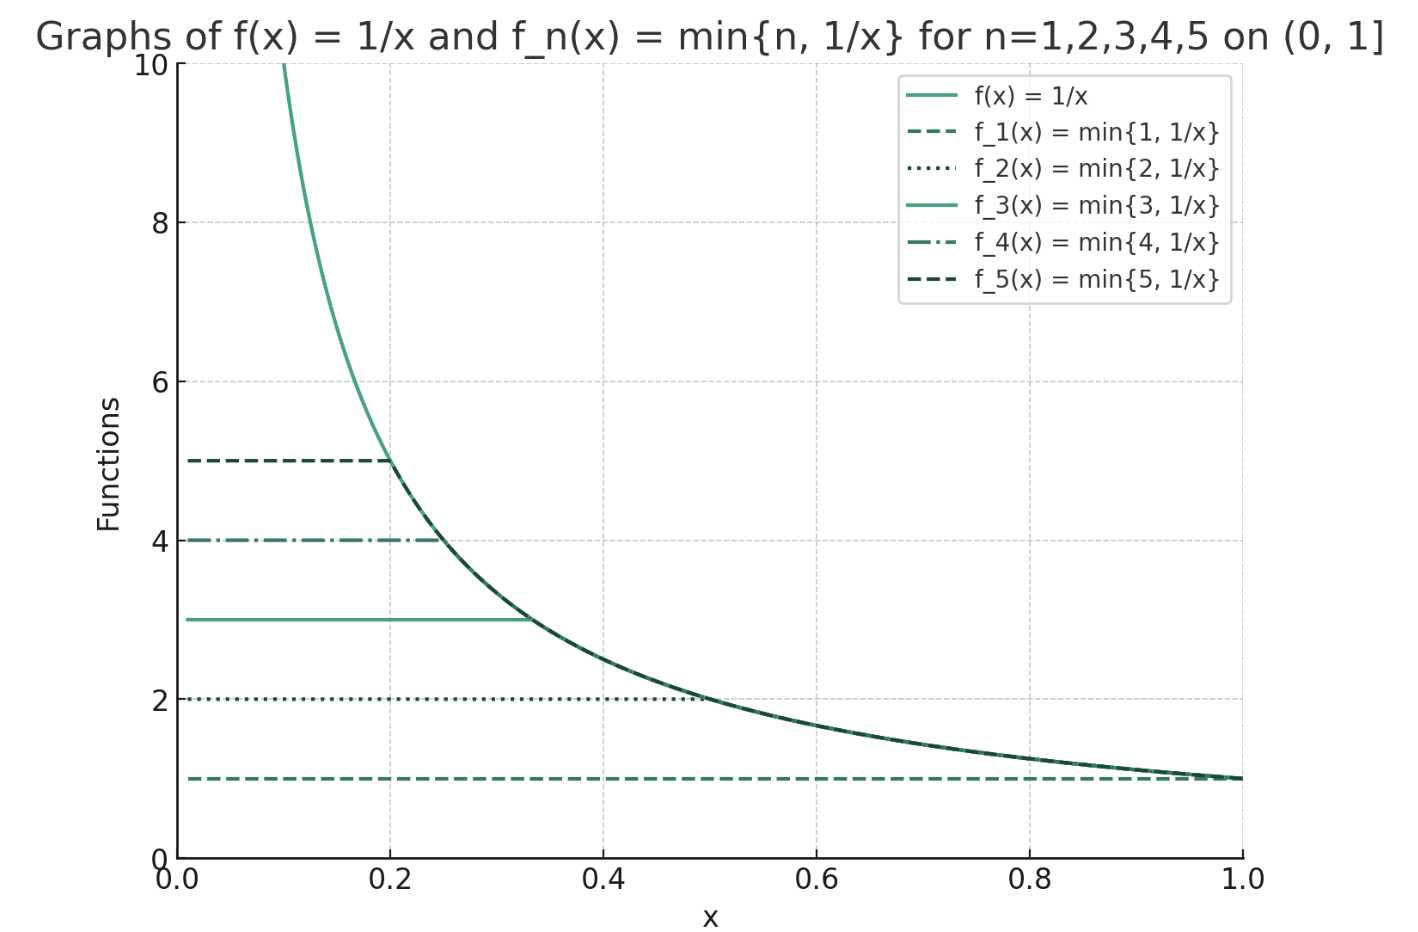
\includegraphics[height=9cm,width=15cm]{pwise converge1.png}
   \end{minipage}
\end{center}
\end{Example}
\begin{Example}{\textbf{(Unbounded functions pointwise converge to bounded function)}}{}
\begin{align*}
X=\R,f_n(x)=\frac{1}{n}x
\end{align*}
The limit function is $f(x)=0$
\begin{center}
   \begin{minipage}{0.9\linewidth}  
       \centering  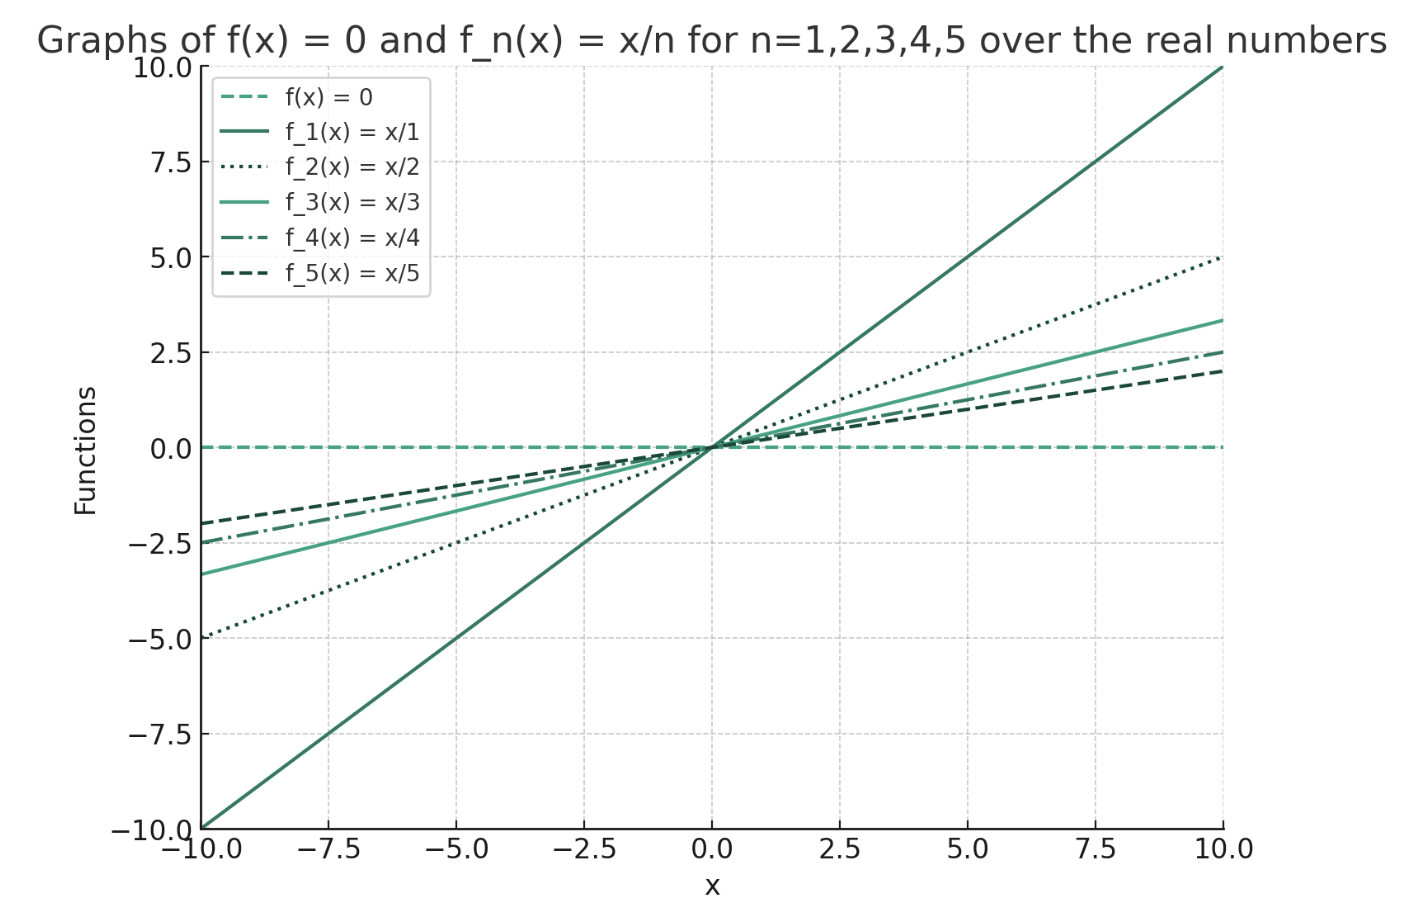
\includegraphics[height=7cm,width=15cm]{pwise converge2.png}
   \end{minipage}
\end{center}
\end{Example}
\end{mdframed} 
\begin{mdframed}
As pointed out earlier, if $f:X\rightarrow (Y,d)$ is bounded and $g:X\rightarrow (Y,d)$ is unbounded, then $d_{\infty}(f,g)=\infty$. This means that if $Y$ is unbounded, the uniform metric $d_{\infty}$ is extended on $X^Y$. For this, it is necessary to develop some basic fact concerning extended metric space.\\

Suppose $(X,d)$ is an extended metric space. If we define $\sim$ on $X$ by $x \sim y\iff  d(x,y)<\infty$, then $\sim $ is an equivalence relation. We say each equivalence class is a \textbf{galaxy} of $(X,d)$. Suppose $T$ is the collection of the galaxies of $(X,d)$. For each $\mathcal{T} \in T$, the space $(\mathcal{T},d)$ is just a metric space.\\

It is easy to see that the way we induce topology from metric space is still valid if the metric is extended. That is 
\begin{align*}
  \tau=\set{Z \in X: \forall z \in Z, \exists \epsilon ,B_\epsilon (z)\subseteq Z}
\end{align*}
is still a topology, even though $d$ is an extended metric on $X$.\\

We can verify that a set $Y$ in $X$ is open if and only if for all  $\mathcal{T} \in T$, the set $Y \cap \mathcal{T}$ is open, and the set $Y$ in $X$ is closed if and only if all convergent sequences $y_n$ in  $Y$ converge to points in $Y$. \\
\end{mdframed}
\begin{mdframed}
Now, suppose we are given an arbitrary set  $X$ and a complete metric space  $(\overline{Y},d)$, and on $X^{\overline{Y}}$, we define the uniform metric  $d_{\infty}$. We say a set $\mathcal{F}\subseteq X^{\overline{Y}}$ of functions is \textbf{closed under uniform convergence} if  for all uniform convergent sequence $f_n \subseteq \mathcal{F}$, the limit function $f$ is also in  $\mathcal{F}$. There are justified reasons for us to give the premise that $\overline{Y}$ is complete prior to the definition of the term \textbf{closed under uniform convergence}. One reason is that by \myref{Theorem}{Tsof}, if $Y$ is not complete, then the extended metric space  $(X^Y,d_{\infty})$ is also not complete, which implies the possibility a Cauchy sequence $f_n$ in  $X^Y$ converge to a function $f \in X^{\overline{Y}} \setminus X^Y$ where $\overline{Y}$ is the completion of  $Y$. For instance, if we let $Y=\R\setminus \set{1}$ where $X=\R$, and let $f_n(x)=\begin{cases}
  0& \text{ if  }x\neq 0\\
  1+\frac{1}{n}& \text{ if $x=0$ }
\end{cases}\in Y$, we see that the set $\mathcal{F}=\set{f_n:n\inn}$ is "closed under uniform convergence" in the context of $X^Y$, but when in fact $f_n$ uniformly converge to  $f(x)=\begin{cases}
  0& \text{ if  }x\neq 0\\
  1& \text{ if $x=0$ }
\end{cases}$ which is not in $\mathcal{F}$. This awkward usage of words can be solved if we define the term  \textbf{closed under uniform convergence} after the premise that $Y$ is complete.\\

Now, given a set of functions $\mathcal{F}\subseteq X^{\overline{Y}}$, one can verify that 
\begin{align*}
  \mathcal{F}\text{ is closed under uniform convergence }&\iff (\mathcal{F},d_{\infty})\text{ is complete }\\
&\iff \mathcal{F}\text{ is closed with respect to $(X^{\overline{Y}},d_{\infty})$ }
\end{align*}
Let $\mathcal{G}$ be a galaxy of $(X^{\overline{Y}},d_{\infty})$. With multiple ways, we can verify that $\mathcal{G}$ is closed with respect to $(X^{\overline{Y}},d_{\infty})$. Then, acknowledging the space of bounded functions $B(X,\overline{Y})$ is a galaxy of $X^{\overline{Y}}$, we see that $B(X,\overline{Y})$ is closed under uniform convergence. The statement that $B(X,\overline{Y})$ is closed under uniform convergence, although already "proved" before as we pointed out the limit of uniform convergent sequence of bounded functions must be bounded, is now in fact actually proved in the sense the term "closed under uniform convergence" is formally given a satisfying definition.
\end{mdframed}
\section{Arzelà–Ascoli Theorem}
\begin{mdframed}
In this section, we will give a complete proof of Arzelà–Ascoli Theorem for functions from arbitrary compact topological space to arbitrary metric space. Note that in Baby Rudin, Arzelà–Ascoli Theorem are given for functions from compact metric space to metric space. Because Arzelà–Ascoli Theorem are concerned with family of equicontinuos functions, it is crucial for us to give a definition to equicontinuity for functions from topological  space to metric space, for the sake of our generalization.\\

Let $X,Y$ be metric space. Let  $Z$ be topological space. Let  $\mathcal{F}_X$ be family of functions from $X$ to  $Y$, and let  $\mathcal{F}_Z$ be family of functions from $Z$ to  $Y$. We say  $\mathcal{F}_Z$ is \textbf{pointwise equicontinuous} if 
\begin{center}
   \begin{minipage}{0.9\linewidth}  
       \centering
       For all $\epsilon $ and for all $x$, there exists a neighborhood $U_x$ such that  $d_Y(f(x),f(y))<\epsilon $ for all $y \in U_x$   
   \end{minipage}
\end{center}
We say $\mathcal{F}_X$ is \textbf{equicontinuous} if 
\begin{center}
   \begin{minipage}{0.9\linewidth}  
       \centering
       For all $\epsilon $, there exists $\delta$ such that  $d_{Y}(f(x),f(y))<\epsilon $ for all $\delta$-close $x,y \in X$ and all  $f \in \mathcal{F}$. 
   \end{minipage}
\end{center}
It is easy to verify that if $\mathcal{F}_X$ is equicontinuous, then $\mathcal{F}_X$ is pointwise equicontinuous. The converse don't always hold true. Say, $\mathcal{F}=\set{n+x^2}_{n\inn}$, the set $\set{n+x^2}_{n\inn}$ is clearly pointwise equicontinuous on $\R$, and is not equicontinuous on $\R$, since no function $n+x^2$  is uniform continuous on $\R$. However, the same set $\mathcal{F}=\set{n+x^2}$ is equicontinous on compact domain $[a,b]$. This is a general result, as we shall prove below.
\end{mdframed}
\begin{theorem}
\textbf{(Pointwise Equicontinous is Uniform on Compact Domain)} Given two metric space $(X,d_X),(Y,d_Y)$, and a family $\mathcal{F}$ of functions from $X$ to  $Y$ such that 
 \begin{enumerate}[label=(\alph*)]
  \item $X$ is compact 
   \item $\mathcal{F}$ is pointwise equicontinuous
\end{enumerate}
Then 
\begin{align*}
\mathcal{F}\text{ is equicontinuous }
\end{align*}
\end{theorem}
\begin{proof}
Fix $\epsilon $. We wish to 
\begin{align*}
\vi{\text{ find $\delta$ such that $d_X(x,y)<\delta \implies d_Y(f(x),f(y))\leq \epsilon $ for all $f \in \mathcal{F}$ }}
\end{align*}
Because $\mathcal{F}$ is pointwise equicontinuous, we know for each $x \in X$, there exists $\delta_x$ such that 
\begin{align}
\label{PEe1}
\forall y\in B_{\delta_x}(x), d_Y\big(f(x),f(y) \big)<\frac{\epsilon}{2} \text{ for all $f\in \mathcal{F}$ }
\end{align}
It is clear that $\set{B_{\frac{\delta_x}{2}}(x):x \in X}$ form an open cover of $X$. Then because  $X$ is compact, we know  
 \begin{align*}
\text{ there exists a finite open sub-cover: }\set{B_{\frac{\delta_x}{2}}(x):x \in X_{\text{finite}}}
\end{align*}
We claim 
\begin{align*}
\vi{\delta=\min_{x \in X_{\text{finite}}}\frac{\delta_x}{2}\text{ works }}
\end{align*}
Fix $y,z \in X: d_X(y,z)<\delta$. We have to prove 
\begin{align*}
\vi{d_Y\big(f(y),f(z) \big)< \epsilon }
\end{align*}
We know $y$ must lie in some  $B_\frac{\delta_x}{2}(x)$ for some $x \in X_\text{finite}$. Because $d_X(y,z)<\frac{\delta_x}{2}$, we see that $z$ must lie in  $B_{\delta_x}(x)$. We now know $y,z$ are both in  $B_{\delta_x}(x)$. Then from \myref{(}{PEe1}), we can now deduce 
\begin{align*}
d_Y\big(f(y),f(z) \big)\leq d_Y\big(f(y),f(x) \big)+d_Y\big(f(x),f(z) \big)< \epsilon \vdone
\end{align*}
\end{proof}
\begin{mdframed}
The proof above should be a great example why in the discussion of metric space, instead of using sequential definition of compactness, which leads to the beautiful Bolzano-Weierstrass Theorem, some people prefer the open-cover definitions.\\

Now, we give proof for the Arzelà–Ascoli Theorem. 
\end{mdframed}
\begin{theorem}
\textbf{(Arzelà–Ascoli Theorem)} Given a compact topological space $(X,\tau)$, a metric space $(Y,d_Y)$, and a family $\mathcal{F}\subseteq C\big(X,Y \big)$ of continuous function  
 \begin{align*}
&\mathcal{F}\text{ is pointwise equicontinuous and $\set{f(x):f \in \mathcal{F}}$ has compact closure in $Y$ for all $x \in X$}\\
&\implies \mathcal{F}\text{ has a compact closure in $C(X,Y)$}
\end{align*}
\end{theorem}
\begin{proof}
Fix a sequence $f_n$ in $\mathcal{F}$. We wish to show
\begin{align*}
\vi{f_n\text{ has a sub-sequence $f_{n_k}$ uniformly converge to some }f:X\rightarrow Y}
\end{align*}
First, we prove 
\begin{align*}
\blue{\text{ there exists a countable set $P$ such that $P$ works like a dense set }}
\end{align*}
Because $\mathcal{F}$ is pointwise equicontinuous, we know for all $x \in X$ 
\begin{align*}
\exists U_{x,n}, \forall y \in U_{x,n},\forall f \in \mathcal{F}, d_Y\big(f(x),f(y) \big)<\frac{1}{n} \text{ for each fixed $n\inn$ }
\end{align*}
Now, because $X$ is compact, for each $n\inn$, there exists a finite subset $P_n\subseteq X$ such that $\bset{U_{x,n}:x \in P_n}$ is a cover of $X$. Let $P=\bigcup_{n\inn}P_n$. $\bdone$\\

Now, we wish to 
\begin{align*}
\olive{\text{ construct a sub-sequence $f_{n_k}$ pointwise converge on $P$ }}
\end{align*}

Express $P=\set{p_k}_{k\inn}$. By premise (pointwise image has compact closure), we know there exists a compact set that contain $\set{f_n(p_1)}_{n\inn}$, so by Bolzano-Weierstrass Theorem, there exists a sub-sequence 
\begin{align*}
\bset{f_{g_1(k)}(p_1)}_{k\inn}\text{ converge to some point in $Y$ }
\end{align*}
Now, again by premise and Bolzano-Weierstrass Theorem, there exists a sub-sequence 
\begin{align*}
\bset{f_{g_2\circ g_1(k)}(p_2)}_{k\inn}\text{ converge to some point in $Y$ }
\end{align*}
Repeatedly doing such, we have 
\begin{align*}
\begin{matrix} 
  f_{g_1(1)}(p_1) & f_{g_2\circ g_1 (1)}(p_2) & f_{g_3\circ g_2 \circ  g_1 (1)}(p_3) & \cdots \\
  f_{g_1(2)}(p_1) & f_{g_2\circ g_1 (2)}(p_2) & f_{g_3\circ g_2 \circ  g_1 (2)}(p_3) & \cdots \\
  f_{g_1(3)}(p_1) & f_{g_2\circ g_1 (3)}(p_2) & f_{g_3\circ g_2 \circ  g_1 (3)}(p_3) & \cdots \\
  \vdots &\vdots &\vdots & \ddots\\
  \downarrow & \downarrow &\downarrow &\\
  y_1 & y_2 & y_3 & \cdots 
\end{matrix}
\end{align*}
Now, let 
 \begin{align*}
n_k=g_k\circ \cdots \circ g_1(k)
\end{align*}
Then 
\begin{align*}
n_k\text{ is eventually a sub-sequence of $g_m\circ \cdots \circ g_1(k)$ for all $m$ }
\end{align*}
This then implies 
\begin{align*}
f_{n_k}(p_m)\to y_m\text{ for all $p_m \in P \odone$ }
\end{align*}
Next, we show 
\begin{align*}
\blue{\text{ To prove $f_{n_k}$ uniformly converge on $X$, it suffice to prove $f_{n_k}$ is uniformly Cauchy on $X$. }}
\end{align*}
By premise (pointwise image has compact closure), if $f_{n_k}$ is uniformly Cauchy, then we know $f_{n_k}$ pointwise converge to some $f$.\\

Fix $\epsilon $. We reduced the problem into 
\begin{align*}
\blue{\text{ finding  $N$ such that for all $k>N$, we have  $d_Y\big(f_{n_k}(x), f(x)\big)\leq \epsilon $ for all $x\in X$ }}
\end{align*}
Because $f_{n_k}$ is uniformly Cauchy, we know there exists $N$ such that for all $m,k>M$ $d_Y\big(f_{n_k}(x),f_{n_m}(x) \big)\leq \frac{\epsilon}{2}$ for all $x \in X$. We claim 
\begin{align*}
 \blue{\text{ such $N$ works }}
\end{align*}
Let $k>N$.  \As{$d_Y\big(f_{n_k}(x),f(x) \big)>\epsilon $}. We see that 
 \begin{align*}
   d_Y\big(f(x),f_{n_m}(x) \big)\geq d_Y\big(f(x),f_{n_k}(x)\big)-d_Y\big(f_{n_k}(x),f_{n_m}(x) \big)>\frac{\epsilon}{2}\text{ for all $m>N\tCaC \bdone$} 
\end{align*}
Lastly, we wish to prove 
\begin{align*}
\vi{f_{n_k}\text{ is uniformly Cauchy }}
\end{align*}
Fix $\epsilon $. We wish  
\begin{align*}
\vi{\text{ to find }N\text{ such that }\forall j,k >N,\forall x\in X, d_Y\big(f_{n_j}(x),f_{n_k}(x)\big)\leq \epsilon  }
\end{align*}
Fix $m > \frac{3}{\epsilon }$. Express $P_m=\set{p^m_1,\dots ,p^m_u}$. Because $f_{n_k}(p^m_t)$ converge for each $t \in \set{1,\dots ,u}$, we know 
\begin{align*}
\forall t , \exists N_t, d_Y\big(f_{n_j}(p_t^m),f_{n_k}(p_t^m) \big)<\frac{\epsilon}{3}\text{ for all $j,k>N_t$ }
\end{align*}
We claim 
\begin{align*}
\vi{N=\max_t N_t\text{ works }}
\end{align*}
Fix $j,k>N$ and $x \in X$. We have to show 
\begin{align*}
  \vi{d_Y\big(f_{n_j}(x),f_{n_k}(x) \big)\leq \epsilon}
\end{align*}
Because $\set{U_{p_t^m,m}}$ form an open cover of $X$, we know there exists  $t$ such that $x \in U_{p_t^m,m}$. We can now deduce 
\begin{align*}
d_Y\big(f_{n_j}(x),f_{n_k}(x) \big)\leq d_Y\big(f_{n_j}(x),f_{n_j}(p_t^m) \big)+d_Y\big(f_{n_j}(p_t^m),f_{n_k}(p_t^m) \big)+d_Y\big(f_{n_k}(p_t^m),f_{n_k}(x) \big)<\epsilon 
\end{align*}
$\vdone$\\

\end{proof}
\section{Banach Fixed Point Theorem}
\begin{mdframed}
This section give a complete statement and proof of Banach Fixed Point Theorem. The setting is 
\begin{enumerate}[label=(\alph*)]
  \item a metric space $\Big(X,d_X \Big)$ 
  \item a subset $E\subseteq X$
  \item another metric space $\Big(Y,d_Y \Big)$ 
  \item a function $f:E\rightarrow Y$ 
  \item another function $g:E\rightarrow X$
\end{enumerate}
We say $f$ is a \textbf{contraction} on $E$ if there exists $r\in [0,1)$ such that 
\begin{align*}
\hspace{3cm}d_Y(f(x),f(y))\leq rd_X(x,y)\hspace{1.5cm}(x,y \in E)
\end{align*}
or equivalently 
\begin{align*}
\sup_{x\neq y \in E} \frac{d_Y(f(x),f(y))}{d_X(x,y)}<1
\end{align*}
Note that the restriction of a contraction is again a contraction. We say $g$ admits a \textbf{fixed point} $x$ if we have 
\begin{align*}
g(x)=x
\end{align*}
\end{mdframed}
\begin{theorem}
\label{BFPT}
\textbf{(Banach Fixed Point Theorem)} If $g$ is a contraction that maps $E$ into $X$, then 
\begin{align*}
g\text{ admits at most one fixed point }
\end{align*}
Moreover, if $E$ is complete and $g(E)\subseteq E$, then 
\begin{align*}
\text{ the fixed point exists }
\end{align*}
And if we use the notation $g^n$ to denote $g\circ g^{n-1}$, then for all $x\in E$,  
\begin{align*}
  \text{ the fixed point can be written in the form }\lim_{n\to \infty}g^n(x)
\end{align*}
\end{theorem}
\begin{proof}
We first 
\begin{align*}
\vi{\text{ prove the uniqueness of the fixed point }}
\end{align*}
Suppose $x,y$ are both fixed by $g$.  We have
\begin{align*}
d(g(x),g(y))=d(x,y)
\end{align*}
Because  $g$ is a contraction mapping,  this implies $d(x,y)=0$. $\vdone$ \\

Suppose $E$ is complete and $g(E)\subseteq E$. We now 
\begin{align*}
\blue{\text{ prove the existence of the fixed point }}
\end{align*}
Fix $x \in E$. Because we have already prove the uniqueness of the fixed point, we only have to prove 
\begin{align*}
\blue{\lim_{n\to \infty}g^n(x)\text{ exists and }\lim_{n\to \infty}g^n(x)\text{ is a fixed point of $g$ }}
\end{align*}
Because $E$ is complete, to prove $\lim_{n\to \infty}g^n(x)$ exists, we only have to prove
\begin{align*}
\olive{\set{g^n(x)}_{n\inn}\text{ is Cauchy }}
\end{align*}
Observe 
\begin{align*}
  d(g^n(x),g^{n+k}(x))&\leq \sum_{i=0}^{k-1}d(g^{n+i}(x),g^{n+i+1}(x))\\
  &\leq d(x,g(x))\sum_{i=0}^{k-1}r^{n+i}\\
  &\leq \frac{r^n}{1-r}d(x,g(x))\to 0\text{ as $n\to \infty$ }\odone
\end{align*}
Note that contraction is Lipschitz thus continuous, and note that $\lim_{n\to \infty}g^n(x) \in E$. This allow us to carry the below limit process 
\begin{align*}
  g\big(\lim_{n\to \infty}g^n(x)\big)=\lim_{n\to \infty}g(g^n(x))=\lim_{n\to \infty}g^{n+1}(x)=\lim_{n\to \infty}g^n(x)\bdone
\end{align*}
\end{proof}
\begin{mdframed}
Banach Fixed Point Theorem is one of the most important Theorem in Mathematics. It will be used to prove 
\begin{enumerate}[label=(\alph*)]
  \item \customref{IFT}{Inverse Function Theorem} 
  \item Picard-Lindelof Theorem  
  \item Nash-Embedding Theorem
\end{enumerate}
\end{mdframed}
\chapter{Algebraic Topology}
\section{Fundamental Group}
\section{Invariance of Domain}
\begin{theorem}
\textbf{(Invariance of Domain)} If $U$ is an open subset of $\R^n$ and  $f:U\rightarrow \R^n$ is one-to-one and continuous, then 
\begin{align*}
f(U)\text{ is open and }f\text{ is a homeomorphism between }U\text{ and }f(U)
\end{align*}
\end{theorem}
\begin{theorem}
\textbf{(Invariance of Dimension)} If $U$ is a non-empty open subset of $\R^n$ and  $V$ is a non-empty subset of $\R^m$ homeomorphic to  $U$, then  $n=m$.
\end{theorem}
\chapter{Linear Algebra Done Outrageous}
\section{Determinant}
\begin{mdframed}
Let $N\triangleq \set{1,\dots,n}$. Given a permutation $\sigma \in S_n$, we say $\sigma$ is \textbf{even} and write $\operatorname{sgn}(\sigma)=1$ if  
\begin{align*}
\set{(x,y)\in N^2:x<y\text{ and }\sigma(x)>\sigma (y)}\text{ has even numbers of element }
\end{align*}
and say $\sigma$ is \textbf{odd} and write $\operatorname{sgn}(\sigma)=-1$ if otherwise. Given some matrix $A\in M(n,R)$, we define its determinant by 
\begin{align*}
\operatorname{det}(A)\triangleq  \sum_{\sigma \in S_n} \operatorname{sgn}(\sigma) A_{\sigma (1),1}\cdots A_{\sigma (n),n} 
\end{align*}
\end{mdframed}
\begin{theorem}
\label{Det}
\textbf{(Determinant)} Let $\set{v_1,\dots ,v_n}$ be a basis for $V$ and  $\set{\omega_1,\dots ,\omega_n}$ be its dual basis. We have
\begin{align*}
\operatorname{sgn}\sigma = \operatorname{det}\Big(\begin{bmatrix}
    \omega_1 v_{\sigma (1)} & \cdots & \omega_1 v_{\sigma (n)}\\
    \vdots & \ddots & \vdots \\
    \omega_n v_{\sigma (1)} & \cdots & \omega_n v_{\sigma (n)}  
\end{bmatrix} \Big) 
\end{align*}
\end{theorem}
\section{Dual Space}
\begin{mdframed}
Given a vector space $V$ over  $\R$, the map  $\alpha :U\rightarrow (U^\vee)^{\vee}$ defined by 
\begin{align*}
\alpha (x)(\rho)\triangleq \rho (x)
\end{align*}
is a vector space isomorphism. Given a linear map $A:V\rightarrow W$, we may define its \textbf{dual map} $A^\vee:W^{\vee}\rightarrow V^{\vee}$ by 
\begin{align*}
A^{\vee}(\xi)(v)\triangleq \xi \circ A(v) 
\end{align*}
\end{mdframed}
\section{Tensor Algebra}
\begin{abstract}
In this section, by the term \textbf{ring}, we mean a ring with a multiplication identity, and by the term \textbf{real algebra}, we mean a real vector space equipped with a vector multiplication compatible with both scalar multiplication and addition. In this definition, for a real algebra $A$ to be a ring, $A$ must be associative.  By the term \textbf{ideal}, we mean a 2-sided ideal. If we say a multi-linear map $M:V^k\rightarrow Z$ is \textbf{alternating}, we mean that $M$ maps $(v_1,\dots ,v_n)$ to $0$ if two arguments coincide.
\end{abstract}
\begin{mdframed}
Given a finite collection $(V_1,\dots ,V_n)$ of finite dimensional real vector space, by the term \textbf{tensor product of $V_1,\dots ,V_n$}, we mean a real vector space  usually denoted by $V_1 \otimes \cdots \otimes  V_n$ and a multilinear map  $\otimes  : V_1 \times \cdots \times V_n \rightarrow V_1 \otimes  \cdots \otimes  V_n$ satisfying the universal property: If $B:V_1 \times \cdots \times V_n\rightarrow Z$ is a multilinear map, then there exists a unique linear map $\beta :V_1\otimes \cdots \otimes  V_n$ such that 
\begin{align*}
B(v_1,\dots ,v_n)=\beta (v_1\otimes \cdots \otimes  v_n)
\end{align*}
In other words, we have the commutative diagram
% https://q.uiver.app/#q=WzAsMyxbMCwwLCJWXFx0aW1lcyBXIl0sWzAsMiwiViBcXG90aW1lcyBXIl0sWzIsMCwiVSJdLFswLDIsIkIiXSxbMSwyLCJcXGV4aXN0cyEgXFxiZXRhIiwyLHsic3R5bGUiOnsiYm9keSI6eyJuYW1lIjoiZGFzaGVkIn19fV0sWzAsMSwiKHYsdylcXG1hcHN0byB2XFxvdGltZXMgdyIsMl1d
\[\begin{tikzcd}
	{V_1\times \cdots \times V_n} && U \\
	\\
	{V_1 \otimes \cdots \otimes   V_n}
	\arrow["B", from=1-1, to=1-3] 
	\arrow["{\otimes }"', from=1-1, to=3-1]
	\arrow["{\exists! \beta}"', dashed, from=3-1, to=1-3]
\end{tikzcd}\]
This approach indeed define a pair of vector space and multilinear map uniquely up to isomorphism, in the sense of \myref{Theorem}{UoT}, where we define the isomorphism between tensor product. 
\end{mdframed}
\begin{theorem}
\label{UoT}
\textbf{(Uniqueness of Tensor product)} Given a finite collection $(V_1,\dots, V_n)$ of finite dimensional real vector space, if $V_1 \otimes \cdots \otimes  V_n ,V_1\otimes  '\cdots \otimes  ' V_n$ both satisfy the universal property, then there exists an linear isomorphism $T:V_1 \otimes  \cdots \otimes  V_n \rightarrow V_1 \otimes' \cdots \otimes  ' V_n $ such that 
\begin{align*}
T(v_1\otimes  \cdots \otimes  v_n)=v_1 \otimes  '\cdots \otimes  'v_n
\end{align*}
\end{theorem}
\begin{proof}
Because $V_1 \otimes  \cdots \otimes  V_n$ satisfies the universal property, there exists a linear map $T:V_1 \otimes  \cdots \otimes  V_n\rightarrow V_1 \otimes'  \cdots \otimes' V_n  $ such that  
\begin{align*}
\otimes' =T \circ \otimes  
\end{align*}
It remains to show $T$ is bijective. Similarly, because $V_1 \otimes ' \cdots \otimes'  V_n$ satisfies the universal property, there exists a linear map $T':V_1 \otimes'  \cdots \otimes'  V_n\rightarrow V_1 \otimes  \cdots \otimes V_n  $ such that 
\begin{align*}
\otimes = T' \circ \otimes  '
\end{align*}
Composing the two equations, we have 
\begin{align*}
\otimes '=T\circ T' \circ \otimes  '
\end{align*}
It then follows from uniqueness of the induced linear map in universal property that $T \circ T'=\textbf{id}:V_1 \otimes  ' \cdots \otimes  'V_n \rightarrow V_1 \otimes  ' \cdots \otimes  'V_n$. This implies $T$ is indeed bijective. 
\end{proof}
\begin{mdframed}
We have shown that tensor products is unique up to isomorphism. A construction further shows that if $B_i$ are bases for $V_i$, then 
 \begin{align*}
\set{v_1 \otimes  \cdots \otimes v_n: v_i \in B_i\text{ for all }1\leq i\leq n  }\text{ form a basis for }V_1 \otimes  \cdots \otimes  V_n
\end{align*}
\end{mdframed}
\begin{theorem}
\textbf{(Associativity of the Tensor product)} Given three finite-dimensional real vector spaces $X,Y,Z$,  there exists a unique linear isomorphism $F:X\otimes  Y\otimes  Z\rightarrow (X\otimes  Y)\otimes  Z$ that satisfy 
\begin{align*}
F(x\otimes  y \otimes  z)=(x\otimes  y)\otimes  z
\end{align*}
\end{theorem}
\begin{proof}
Define $f:X\times Y \times Z\rightarrow (X\otimes  Y)\otimes Z$ by 
\begin{align*}
f(x,y,z)\triangleq (x \otimes  y)\otimes z
\end{align*}
It follows from the universal property that there exists a unique linear map $F:X\otimes  Y\otimes Z\rightarrow (X \otimes  Y)\otimes  Z $ such that 
\begin{align*}
F(x\otimes  y\otimes  z)=f(x,y,z)= (x \otimes y) \otimes z 
\end{align*}
It remains to show \vi{$F$ is bijective}.  For all $z\in Z$, define $h_z:X\times Y\rightarrow X \otimes  Y\otimes Z$ by 
\begin{align*}
h_z(x,y)\triangleq x\otimes  y\otimes  z
\end{align*}
If follows from the universal property that there exists a unique linear map $H_z:X\otimes  Y \rightarrow X \otimes  Y\otimes  Z$ such that 
\begin{align*}
H_z(x \otimes  y)=h_z(x,y)=x \otimes  y \otimes  z
\end{align*}
Define $h:(X\otimes  Y)\times Z\rightarrow X\otimes Y \otimes Z$ by 
\begin{align*}
h(v,z)\triangleq H_z(v)
\end{align*}
It is clear that $h$ in linear in  $(X\otimes  Y)$. We now show $h$ is linear in  $Z$, that is 
 \begin{align*}
   \olive{H_{c_1z_1+z_2}=c_1H_{z_1}+H_{z_2}}
\end{align*}
By definition, 
\begin{align*}
  (c_1H_{z_1}+H_{z_2})(x\otimes  y)&=c_1 x\otimes  y\otimes  z_1+ x\otimes  y \otimes  z_2\\
  &= x\otimes  y\otimes  (c_1z_1+z_2)=h_{c_1z_1+z_2}(x,y)
\end{align*}
It then follows from the uniqueness part of the universal property that $H_{c_1z_1+z_2}=c_1H_{z_1}+H_{z_2}$. $\odone$  \\


We have shown $h$ is indeed bilinear. It follows from the universal property that there exists a unique linear map $H:(X\otimes  Y)\otimes  Z\rightarrow X\otimes Y\otimes Z$ such that 
\begin{align*}
H((x\otimes y)\otimes z)=h(x\otimes  y,z)=H_z(x\otimes  y)=x\otimes  y\otimes  z
\end{align*}
Let $\otimes:X\times Y\times Z\rightarrow X\otimes  Y\otimes  Z$ denotes the tensor product, we now have 
\begin{align*}
\otimes = H \circ F \circ \otimes 
\end{align*}
It then follows from universal property that $H \circ F=\textbf{id}:X\otimes  Y\otimes  Z\rightarrow X\otimes  Y\otimes  Z$. This implies $F$ is indeed bijective. $\vdone$
\end{proof}
\begin{mdframed}
Let $V$ be a finite-dimensional real vector space. By its  \textbf{tensor algebra}, we mean any real associative algebra $T(V)$ with an injective linear map $\diota:V\rightarrow T(V)$ that satisfies the universal property: If $A$ is a real associative algebra and $f:V\rightarrow A$ is a linear map, then there exists a unique algebra homomorphism $F:T(V)\rightarrow A$ such that the diagram  
% https://q.uiver.app/#q=WzAsMyxbMiwwLCJUKFYpIl0sWzIsMiwiQSJdLFswLDAsIlYiXSxbMiwwLCJcXGRvdHtcXGlvdGF9Il0sWzIsMSwiZiIsMl0sWzAsMSwiRiIsMCx7InN0eWxlIjp7ImJvZHkiOnsibmFtZSI6ImRhc2hlZCJ9fX1dXQ==
\[\begin{tikzcd}
	V && {T(V)} \\
	\\
	&& A
	\arrow["{\dot{\iota}}", from=1-1, to=1-3]
	\arrow["f"', from=1-1, to=3-3]
	\arrow["F", dashed, from=1-3, to=3-3]
\end{tikzcd}\]
commutes. The proof that such definition is indeed unique up to isomorphism is similar to that of \myref{Theorem}{UoT} and thus omitted. We now give the most useful construction. \\

Let $V$ be finite-dimensional real vector space. We use the notation 
 \begin{align*}
T^n(V)\triangleq  \overbrace{V \otimes  \cdots \otimes  V}^{n\text{ copies }}
\end{align*}
and call $T^{n}(V)$ the \textbf{$n$-th tensor power of $V$} or the \textbf{$n$-fold tensor product of  $V$}. Define  
\begin{align*}
  T(V)&\triangleq  \bigoplus_{n=0}^{\infty} T^n(V)\\
  &=\R \oplus V \oplus (V\otimes V) \oplus (V\otimes V \otimes V)  \oplus \cdots 
\end{align*}
and define for all $f,g \in T(V)$ the multiplication 
\begin{align*}
  (fg)(n)\triangleq   \sum_{k=0}^{n}f(k)g(n-k)
\end{align*}
where 
\begin{align*}
  &\Big(\sum_{I} a_I v_{I(1)}\otimes \cdots \otimes  v_{I(k)}\Big)\Big(\sum_J b_J v_{J(1)}\otimes  \cdots \otimes  v_{J(l)}\Big)\\
  &\triangleq \sum_{I,J} a_I b_J v_{I(1)}\otimes \cdots \otimes  v_{I(k)}\otimes  v_{J(1)}\otimes  \cdots \otimes  v_{J(l)}
\end{align*}
where $\set{v_1,\dots ,v_m}$ is some basis for $V$, $I$ run through the set of function that maps $\set{1,\dots ,k}$ into $\set{1,\dots ,m}$ and $J$ run through the set of function that maps  $\set{1,\dots ,l}$ into $\set{1,\dots ,m}$. For example, given two elements  
\begin{align*}
  (5,0,v_1\otimes v_2,0,0,\dots )\text{ and }(7,v_3,0,0,\dots)
\end{align*}
of $T(V)$, their product is defined to be 
\begin{align*}
  (35,5v_3,7v_1\otimes v_2, v_1 \otimes v_2 \otimes v_3 ,0,0,\dots)
\end{align*}
Tedious effort shows that our multiplication is consistent with abuse of notation in the sense that if $f,g\in T(V)$ is defined by  
\begin{align*}
 f(k)\triangleq \begin{cases}
   w_1\otimes \cdots \otimes  w_n & \text{ if $k=n$ }\\
   0& \text{ if otherwise }
 \end{cases} \text{ and } g(k)\triangleq \begin{cases}
   w_{n+1}\otimes  \cdots \otimes  w_{n+l}& \text{ if $k=l$ }\\
   0& \text{ if otherwise }
 \end{cases} 
\end{align*}
then 
\begin{align*}
  (fg)(k)=\begin{cases}
    w_1\otimes  \cdots \otimes  w_{n+l}& \text{ if $n=k+l$ }\\
    0& \text{ if otherwise }
  \end{cases}
\end{align*}


does form an associative algebra with multiplication identity $1\inr$. Thus, $T(V)$ is in fact a ring. Let $I(V)\subseteq T(V)$ be the ideal generated by $\set{v\otimes v:v \in V}$. By definition, ideal $I(V)$ is a subgroup of $T(V)$. To see that $I(V)$ is closed under scalar multiplication, observe that for all $t\inr\text{ and }x\in T(V)$, the scalar multiplication $tx$ is identical to $tx$ where $t$ is treated as an element of $T(V)$, so it follows from definition of ideal that $I(V)$ is also a vector subspace of $T(V)$. Let $\set{v_1,\dots ,v_n}$ be a basis for $V$, and let  $S$ be the set of function that maps  $\set{1,\dots ,n}$ into $\set{1,\dots ,k}$. We know for a fact that 
\begin{align*}
T^k(V) = \operatorname{span} \set{v_{I(1)}\otimes  \cdots \otimes  v_{I(k)}: I \in S}
\end{align*}
If we define $I^k(V)\triangleq I(V)\cap T^k(V)$, one then have 
\begin{align}
\label{ikv} I^k(V)=\operatorname{span}\set{v_{I(1)}\otimes \cdots \otimes  v_{I(k)}:I(j)=I(j+1)\text{ for some }j}
\end{align}
This is proved by showing $I^0(V)\oplus  I^1(V)\oplus  I^2(V)\oplus  \cdots $ is indeed the smallest ideal containing $\set{v\otimes  v:v \in V}$. Define an equivalence class on $T(V)$ by 
\begin{align*}
x\sim  y\overset{\triangle}{\iff }x-y \in I (V)
\end{align*}
Because ideal form a subgroup, we see that our definition indeed give an equivalence relation. We then can define on the set of equivalence class $T(V)\setminus I(V)$ addition, scalar multiplication and vector multiplication 
\begin{align*}
[x]+[y]\triangleq [x+y] \text{ and }[x]\wedge [y]\triangleq [xy]\text{ and }c[x]\triangleq [cx]
\end{align*}
which is well defined and form an algebra as one can check. We call this algebra $T(V)\setminus I(V)$ the \textbf{exterior algebra} $\wedge ^* (V)$. Note that if we refer to $v,w \in T^k(V)$ as elements of $\wedge ^*(V) $, we mean $[v],[w]$. Immediately, we see that the wedge product is \textbf{alternating} in the sense that if $v\in V$, then 
\begin{align*}
v\wedge v=0 
\end{align*}
and is \textbf{anti-symmetric} in the sense that if $v,w \in V$, then 
\begin{align*}
v\wedge w= -w\wedge  v
\end{align*}
We use the notation 
\begin{align*}
\wedge^k(V) \triangleq \bset{ [x] \in \wedge ^*(V): x \in \overbrace{V \otimes  \cdots \otimes  V}^{k\text{ copies }}} 
\end{align*}
Immediately from \myref{Equation}{ikv}, we see that $\wedge ^k (V) $ is the vector space 
\begin{align*}
\operatorname{span}\set{v_{I(1)}\wedge  \cdots \wedge  v_{I(k)}:I \in S  }
\end{align*}
where $\set{v_1,\dots ,v_n}$ is a basis for $V$ and $S$ is the set of function that maps  $\set{1,\dots ,k}$ into $\set{1,\dots ,n}$. If we define the vector subspace $I^k(V)\triangleq T^k(V)\cap I(V)$, there exists a natural vector space isomorphism
\begin{align*}
\wedge  ^k(V)\underset{\text{ v.s. }}{\cong }T^k(V)\setminus I^k(V);[x]\leftrightarrow [x]
\end{align*}
where $T^k(V)\setminus I^k(V)$ is the quotient vector space.
\end{mdframed}
\begin{theorem}
\label{Universal mapping property for alternating $k$-linear map}
\textbf{(Universal mapping property for alternating $k$-linear map)} For any vector space $Z$ over  $\R$ and any alternating  $k$-linear map  $f:V^k\rightarrow Z$, there is a unique linear map $F:\bigwedge ^k V\rightarrow Z $ such that the diagram 
% https://q.uiver.app/#q=WzAsMyxbMCwwLCJcXGJpZ3dlZGdlXmsgViAiXSxbMCwyLCJWXmsiXSxbMiwyLCJaIl0sWzEsMCwiXFx3ZWRnZSAiXSxbMCwyLCJcXHRpbGRle2Z9Il0sWzEsMiwiZiIsMl1d
\[\begin{tikzcd}
	{\bigwedge^k V } \\
	\\
	{V^k} && Z
	\arrow["F", from=1-1, to=3-3]
	\arrow["{\wedge }", from=3-1, to=1-1]
	\arrow["f"', from=3-1, to=3-3]
\end{tikzcd}\]
commute, i.e., 
\begin{align*}
F(v_1\wedge \cdots \wedge  v_k  )=f(v_1,\dots ,v_k) \text{ for all }v_1,\dots,v_k \in V
\end{align*}
\end{theorem}
\begin{proof}
By \customref{Universal Property of Tensor Product}{universal property of tensor product}, there exists unique linear map $h:T^k(V)\rightarrow Z$ such that 
 \begin{align*}
h(v_1 \otimes  \cdots \otimes  v_k)=f(v_1,\cdots ,v_k)
\end{align*}
Because $f$ is alternating, we see from the characterization of $I^k(V)$ given in \myref{Equation}{ikv} that $h$ vanishes on $I^k(V)$. We then can induce a linear map 
\begin{align*}
F:\wedge^k (V)\cong \frac{T^k(V)}{I^k(V)} \rightarrow Z 
\end{align*}
by $F([x])\triangleq h(x)$. This then give us the desired  
\begin{align*}
F(v_1 \wedge  \cdots \wedge  v_k )=h(v_1\otimes  \cdots \otimes  v_k)=f(v_1,\dots ,v_k)
\end{align*}
Note that $F$ is unique because all such linear map take the same values on  $\set{v_{I(1)}\wedge  \cdots \wedge  v_{I(k)}:I \in S }$ which spans $\wedge ^k(V) $. 
\end{proof}
\begin{mdframed}
Let $\set{w_1,\dots ,w_l}\subseteq V$ be linear independent. An immediate consequence of the \customref{Universal mapping property for alternating $k$-linear map}{universal mapping property for alternating $k$-linear map} is that one may define alternating multilinear $f:V^l\rightarrow \R$ by 
\begin{align*}
B(v_1,\dots ,v_l)\triangleq \operatorname{det}(M)\text{ where }v_i= \sum_j M_{i,j}w_j
\end{align*}
and see that $F:\wedge^l (V)\rightarrow \R $ take $w_1\wedge  \cdots \wedge  w_l$ to $1$. This implies that  
\begin{align*}
w_1\wedge  \cdots \wedge  w_l \neq 0  
\end{align*}
\end{mdframed}
\begin{theorem}
\label{ASo}
\textbf{(Anti-symmetry of wedge product)} If $\alpha \in \wedge ^k (V),\beta \in \wedge ^l (V)  $, then $\alpha \wedge  \beta =(-1)^{kl}(\beta  \wedge  \alpha  )  $. 
\end{theorem}
\begin{proof}
Let $v_1,\dots ,v_n$ be a basis of $V$. Let $S_k$ be the space of function that maps $\set{1,\dots ,k}$into  $\set{1,\dots,n}$ , $S_l$ be the space of function that maps  $\set{1,\dots ,l}$ into  $\set{1,\dots ,n}$. We may then write 
\begin{align*}
\alpha = \sum_{I \in S_k} a_I (v_{I(1)}\wedge \cdots \wedge  v_{I(k)})\text{ and }\beta =\sum_{J \in S_l} b_J (v_{J(1)}\wedge \cdots \wedge v_{J(l)}  )
\end{align*}
and compute 
\begin{align*}
\alpha \wedge \beta &= \sum_{I \in S_k,J\in S_l}a_Ib_J (v_{I(1)}\wedge \cdots \wedge v_{I(k)} \wedge  v_{J(1)} \wedge \cdots  \wedge v_{J(l)}   )\\
&=   \sum_{I \in S_k,J\in S_l}(-1)a_Ib_J (v_{I(1)}\wedge \cdots \wedge   v_{J(1)} \wedge  v_{I(k)}\cdots\wedge \cdots  \wedge v_{J(l)}   )   \\
&=  \sum_{I \in S_k,J\in S_l}(-1)^ka_Ib_J (v_{J(1)}\wedge v_{I(1)}\wedge  \cdots \wedge    v_{I(k)} \wedge  v_{J(2)} \wedge \cdots  \wedge v_{J(l)}   )   \\
  &=\sum_{I \in S_k,J\in S_l}(-1)^{kl}a_Ib_J (v_{J(1)}\wedge \cdots \wedge  v_{J(l)}\wedge v_{I(1)} \wedge   \cdots \wedge   v_{I(k)})= (-1)^{kl}\beta \wedge  \alpha  
\end{align*}
\end{proof}
\begin{mdframed}
Following from \myref{Theorem}{ASo}, \myref{Equation}{ikv} and tedious effort, one can see that if $\set{v_1,\dots ,v_n}$ is a basis for $V$, then 
 \begin{align*}
\set{v_{i_1}\wedge  \cdots \wedge  v_{i_k}:1\leq i_1< \cdots < i_k\leq n  }
\end{align*}
form a basis for $\wedge^k(V)$. If $A:V\rightarrow W$ is a linear map, we define linear map $\wedge^k A:\wedge^k (V)\rightarrow \wedge^k (W) $ by linear extension of 
\begin{align*}
\wedge^k(A)(v_1\wedge  \cdots \wedge   v_n)=Av_1 \wedge  \cdots \wedge  Av_n  
\end{align*}
Note that if  $A:V\rightarrow V$ and $\operatorname{dim}(V)=n$, then $\wedge ^nA: \wedge^n (V)\rightarrow \wedge ^n(V)$ is given by the determinant since given basis  $\set{v_1,\dots ,v_n}$, we have 
\begin{align*}
\wedge^nA(v_1 \wedge  \cdots \wedge  v_n   )&=\Big(\sum_j A_{j,1}v_j\Big)\wedge  \cdots \wedge \Big(\sum_j A_{j,n}v_j\Big)    \\
&=\sum_{\sigma \in S_n} A_{\sigma (1),1}\cdots A_{\sigma (n),n}v_{\sigma (1)}\wedge  \cdots \wedge  v_{\sigma(n)}   \\
&=\sum_{\sigma \in S_n}\operatorname{sgn}(\sigma)A_{\sigma(1),1}\cdots A_{\sigma(n),n}v_1\wedge  \cdots \wedge  v_n
\end{align*}
\end{mdframed}
\section{Norm and Inner Product}
\begin{mdframed}
This section contains
\begin{enumerate}[label=(\alph*)]
  \item definition and basic properties of the term \textbf{norm}
  \item definition and basic properties of the term \textbf{inner product}
  \item definition and basic properties of the term \textbf{positive semi-definite Hermitian form}
  \item full statement and proof of \textbf{Cauchy Schwarz Inequality} for both inner product space and positive semi-definite Hermitian form  
  \item statement and proof of \textbf{SVD} (singular value decomposition). 
\end{enumerate}
\end{mdframed}
\textbf{(Norm Axiom Part)}
\begin{mdframed}
Recall that by a \textbf{normed space} $V$, we mean a vector space over a sub-field $\F$ of $\C$ equipped with  $\norm{\cdot}:V\to \R_0^+$ satisfying the following $\underline{\text{axioms}}$: 
\begin{enumerate}[label=(\alph*)]
  \item $\norm{x}=0 \implies x=0$ (positive-definiteness)
  \item $\norm{sx}=\abso{s}\cdot \norm{x}$ for all $s \in \F$ and $x\in V$ (absolute-homogenity)
  \item $\norm{x+y}\leq \norm{x}+\norm{y}$ for all $x,y \in V$ (triangle inequality)
\end{enumerate}
Observe
\begin{align*}
\norm{0}=\norm{0+x}\leq \norm{0}+\norm{x}\text{ for all $x\in V$ }
\end{align*}
This shows that $\norm{x}\geq 0$ for all $x\in V$. Also observe 
\begin{align*}
\norm{0}=\norm{0(x)}=\abso{0}\cdot \norm{x}=0
\end{align*}

We can now rewrite the normed space axioms into
\begin{enumerate}[label=(\alph*)]
  \item $\norm{x}=0\iff x=0$ (positive-definiteness)
  \item $\norm{sx}=\abso{s}\cdot \norm{x}$ for all $s \in \F$ and $x\in V$ (absolute-homogeneity)
  \item $\norm{x+y}\leq \norm{x}+\norm{y}$ for all $x,y \in V$ (triangle inequality)
  \item $\norm{x}\geq 0$ for all $x \in V$ (non-negativity)
\end{enumerate}
\end{mdframed}
\textbf{(Inner Product Axiom Part)}
\begin{mdframed}
Recall that by an \textbf{inner product space} $V$, we mean a vector space over  $\R$ or $\C$ equipped with  $\langle \cdot,\cdot\rangle : V^2 \rightarrow \R\text{ or }\C$ satisfying the following $\underline{\text{axioms}}$
\begin{enumerate}[label=(\alph*)]
  \item $\langle x,x\rangle >0$ for all $x\neq 0$ (Positive-definiteness)
  \item $\langle x,y\rangle =\overline{\langle y,x\rangle }$ (Conjugate symmetry)
  \item $\langle x+y,z\rangle =\langle x,z\rangle +\langle y,z\rangle $ and $\langle cx,z\rangle=c\langle x,z\rangle $ (Linearity in the first argument)
\end{enumerate}
Note that conjugate symmetry let us deduce
\begin{align*}
\langle x,x\rangle =\overline{\langle x,x\rangle }\implies \langle x,x\rangle \inr
\end{align*}
Also, one can easily use linearity in first argument to deduce 
\begin{align*}
\langle 0,0\rangle =2\langle 0,0\rangle \implies \langle 0,0\rangle =0
\end{align*}
This now let us rewrite the inner product space over $\C$ axioms into 
\begin{enumerate}[label=(\alph*)]
  \item $\langle x,x\rangle \geq 0$ for all $x\in V$ (non-negativity) 
  \item $\langle x,x\rangle =0 \iff x=0$ (positive-definiteness)
  \item $\langle x,y\rangle =\overline{\langle y,x\rangle }$ (conjugate symmetry)
  \item $\langle cx+y,z\rangle =c\langle x,z\rangle +\langle y,z\rangle $ and $\langle x,cy+z\rangle =\overline{c}\langle x,y\rangle +\langle x,z\rangle $ (Linearity)
\end{enumerate}
Note that using $c=1$ and $y=0$, ($\because \langle 0,z\rangle =0\langle x,z\rangle=0 $) one can check that the latter expression of linearity implies the first expression.
\end{mdframed}
\begin{mdframed}
If the scalar field is $\R$, then conjugate symmetry is just symmetry and we also have linearity in the second argument.\\

This now let us rewrite the inner product space over $\R$ axioms into 
\begin{enumerate}[label=(\alph*)]
  \item $\langle x,x\rangle \geq 0$ for all $x\in V$ (non-negativity) 
  \item $\langle x,x\rangle =0 \iff x=0$ (positive-definiteness)
  \item $\langle x,y\rangle =\langle y,x\rangle $ (symmetry)
  \item Linearity in both arguments
\end{enumerate}
\end{mdframed}
\begin{mdframed}
If we do not require $\langle \cdot,\cdot\rangle $ to be positive-definite, but only non-negative, i.e. $\langle x,x\rangle \geq 0$ for all $x\in V$, then we have a \textbf{positive semi-definite Hermitian form}. Formally speaking, a positive semi-definite Hermitian form $\langle\cdot,\cdot \rangle :V^2 \rightarrow \R\text{ or }\C$ satisfy the following axioms
\begin{enumerate}[label=(\alph*)]
  \item $\langle x,x\rangle \geq 0$ for all $x\in V$ (non-negativity)
  \item $\langle x,y\rangle =\overline{\langle y,x\rangle }$ (conjugate symmetry)
  \item $\langle x+y,z\rangle =\langle x,z\rangle +\langle y,z\rangle $ and $\langle cx,z\rangle=c\langle x,z\rangle $ (Linearity in the first argument)
\end{enumerate}
\begin{Example}{\textbf{(Example of Positive semi-definite Hermitian form)}}{}
\begin{align*}
\text{ arbitrary }V\text{ over $\R$ or  $\C$ }\hspace{0.5cm}\langle x,y\rangle \triangleq 0\text{ for all $x,y$ }\hspace{1cm}
\end{align*}
\end{Example}
\end{mdframed}
\textbf{(Norm Induce Part)}
\begin{mdframed}
Given a vector space $V$ over $\R$ or  $\C$, one can check that if  $V$ is equipped with an inner product  $\langle \cdot,\cdot\rangle :V^2\rightarrow \R\text{ or }\C$, then we can induce a norm on $V$ by 
\begin{align*}
\hspace{3cm}\norm{x}\triangleq \sqrt{\langle x,x\rangle }\hspace{1.5cm}(x \in V)
\end{align*}
Note that 
\begin{align*}
\norm{x}=0\iff \langle x,x\rangle =0 
\end{align*}
This implies that if $\langle \cdot,\cdot\rangle $ is an inner product (satisfy positive-definiteness), then $\norm{\cdot}$ is also positive-definite. And if $\langle \cdot,\cdot\rangle $ is not positive-definite, then there exists  $x\neq 0\in V$ such that $\norm{x}=0$, which make $\norm{\cdot}$ a \textbf{semi-norm}.\\

Absolute homogeneity follows from the linearity of inner product.\\

To check triangle inequality, we first have to prove Cauchy-Schwarz inequality.
\end{mdframed}
\begin{theorem}
\label{BPoP}
\textbf{(Basic Property of Positive semi-definite Hermitian form)} Given a positive semi-definite Hermitian form $\langle \cdot,\cdot\rangle:V^2 \rightarrow \R\text{ or }\C $ and $x,y \in V$, we have 
\begin{align*}
\langle x,x\rangle =0 \implies \langle x,y\rangle =0
\end{align*}
\end{theorem}
\begin{proof}
\As{$\langle x,y\rangle\neq 0 $}. Fix $t> \frac{\norm{y}^2 }{2\abso{\langle x,y\rangle }^2}$. Compute 
\begin{align*}
\norm{y-t\langle y,x\rangle x}^2 &= \norm{y}^2 + \norm{(-t)\langle y,x\rangle x }^2  + \langle -t\langle y,x\rangle x,y \rangle + \langle y,-t\langle y,x\rangle x\rangle \\
&=\norm{y}^2 + t^2 \abso{\langle x,y\rangle }^2 \norm{x}^2 -t \langle y,x\rangle \langle x,y\rangle - t \langle x,y\rangle \langle y,x\rangle  \\
&= \norm{y}^2- 2t \abso{\langle x,y\rangle }^2 <0 \tCaC
\end{align*}
\end{proof}
\begin{theorem}
\label{CSI}
\textbf{(Cauchy-Schwarz Inequality)} Given a positive semi-definite Hermitian form $\langle \cdot,\cdot\rangle :V^2\rightarrow \C$ on vector space $V$ over $\C$, we have 
\begin{enumerate}[label=(\alph*)]
  \item $\abso{\langle x,y\rangle}\leq  \norm{x}\cdot\norm{y}\hspace{0.5cm}(x,y \in V)$ 
  \item the equality hold true if $x,y$ are linearly dependent
  \item the equality hold true if and only if $x,y$ are linearly dependent (provided $\langle \cdot,\cdot\rangle $ is an inner product)
\end{enumerate}
\end{theorem}
\begin{proof}
We first prove 
\begin{align*}
  \vi{\hspace{3cm}\abso{\langle x,y\rangle }\leq \norm{x}\cdot\norm{y}\hspace{1.5cm}(x,y \in V)}
\end{align*}
Fix $x,y \in V$. \myref{Theorem}{BPoP} tell us $\norm{x}=0 \implies  \langle x,y\rangle =0$. Then we can reduce the problem into proving 
\begin{align*}
\vi{\frac{\abso{\langle x,y\rangle }^2}{\norm{x}^2}\leq\norm{y}^2  }
\end{align*}
Set $z\triangleq y-\frac{\langle y,x\rangle }{\norm{x}^2}x$. We then have 
\begin{align*}
\langle z,x\rangle =\langle y-\frac{\langle y,x\rangle }{\norm{x}^2}x,x \rangle =\langle y,x\rangle - \frac{\langle y,x\rangle }{\norm{x}^2}\langle x,x\rangle =0
\end{align*}
Then from $y=z+\frac{\langle y,x\rangle }{\norm{x}^2}x$, we can now deduce
\begin{align*}
\langle y,y\rangle &= \langle z+\frac{\langle y,x\rangle }{\norm{x}^2}x,z+ \frac{\langle y,x\rangle }{\norm{x}^2}x\rangle  \\
&=\langle z,z\rangle + \abso{\frac{\langle y,x\rangle }{\langle x,x\rangle }}^2 \langle x,x\rangle \\
&=\langle z,z\rangle + \frac{\abso{\langle x,y\rangle }^2}{\langle x,x\rangle }
\end{align*}
Because $\langle z,z\rangle\geq 0 $, we now have
\begin{align*}
\langle y,y\rangle = \langle z,z\rangle + \frac{\abso{\langle x,y\rangle }^2}{\langle x,x\rangle }\geq  \frac{\abso{\langle x,y\rangle }^2}{\langle x,x\rangle }\vdone
\end{align*}
The equality hold true if and only if $\langle z,z\rangle =0$. This explains the other two statements regarding the equality. 
\end{proof}
\begin{mdframed}
The proof is clearly geometrical. If one wish to remember the proof, one should see the trick we use is exactly 
\begin{align*}
z\triangleq y-\abso{y}(\cos \theta )\hat{x}\text{ is the projection of $y$ onto $x^{\perp}$ }
\end{align*}
\begin{center}
   \begin{minipage}{0.9\linewidth}  
       \centering
       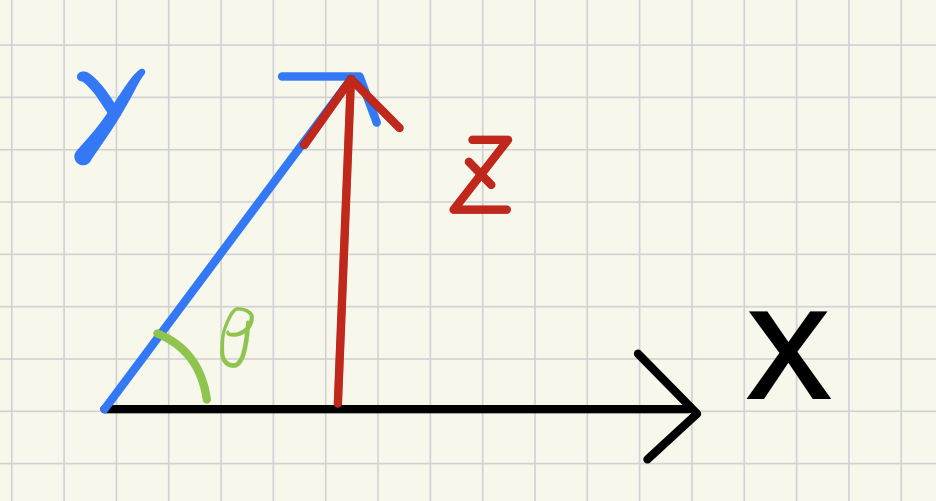
\includegraphics[height=5cm,width=12cm]{CSp.jpeg}
   \end{minipage}
\end{center}
Then all we do rest is just expanding $\abso{y}^2=\abso{z+\tilde{x}}^2$, where $\tilde{x}=y-z=\abso{y}(\cos \theta)\hat{x}$, which give the answer and is easy to compute since $z\cdot \tilde{x}=0$.\\

Now, with Cauchy-Schwarz Inequality, we can check the triangle inequality 
\begin{align*}
  \norm{x+y}^2&=\langle x+y,x+y\rangle \\
&=\langle x,x\rangle +\langle x,y\rangle +\langle y,x\rangle +\langle y,y\rangle \\
&= \langle x,x\rangle + \langle y,y\rangle +2\text{ Re }\langle x,y\rangle \\
&\leq \norm{x}^2 + \norm{y}^2 + 2\abso{\langle x,y\rangle }\\
&\leq \norm{x}^2 + \norm{y}^2 + 2\norm{x}\cdot \norm{y}=\Big(\norm{x}+\norm{y}\Big)^2
\end{align*}
\end{mdframed}
\textbf{(Euclidean Space Abstract Part)} 
\begin{mdframed}
  By a \textbf{concrete Euclidean Space}, we mean some space of $n$-tuple  $(x_1,\dots ,x_n)$ over $\R$, equipped with inner product  $\langle \cdot,\cdot\rangle_E$ defined by 
\begin{align*}
  \langle  (x_1,\dots,x_n)  ,(y_1,\dots ,y_n)\rangle_E= \sqrt{\sum_{k=1}^n (y_k-x_k)^2} 
\end{align*}
By an \textbf{Euclidean Space}, we simply mean a finite dimensional vector space $V$ over $\R$,  equipped with an inner product $\langle \cdot,\cdot\rangle $ such that there exists a concrete Euclidean space $E$ and an isomorphism  $\phi:V\to E$ such that 
\begin{align*}
\hspace{3cm}\langle x,y\rangle= \langle \phi (x),\phi (y)\rangle_E \hspace{1.5cm}(x,y \in V)
\end{align*}
Note that if you define $\langle \cdot,\cdot\rangle $ on the space of $n$-tuples $(x_1,\dots ,x_n)$ over $\R$ by 
\begin{align*}
  \langle  (x_1,\dots,x_n)  ,(y_1,\dots ,y_n)\rangle=2 \sqrt{\sum_{k=1}^n (y_k-x_k)^2} 
\end{align*}
Then, the space of $n$-tuple is clearly not a concrete Euclidean space, and clearly an Euclidean space. 

\end{mdframed}
\textbf{(SVD)}

\chapter{Differential Calculus}
\section{Operator Norm}
\begin{abstract}
This section introduces the concept of the operator norm and proves some fundamental results related operator norm and finite-dimensional normed spaces. For example, we establish results such as \customref{LOB}{a linear operator being bounded if and only if it is continuous} and \customref{ANoF}{the equivalence of all norms on finite-dimensional vector spaces}.
\end{abstract}
\begin{mdframed}
In this section, and particularly in functional analysis, we say a function $T$ between two metric space is a  \textbf{bounded operator} if $T$ always map bounded set to bounded set. In particular, if $T$ is a linear transformation between two normed space, we say $T$ is a \textbf{bounded linear operator}. Now, suppose $\mathcal{X},\mathcal{Y}$ are two normed space over $\R\text{ or }\C$. In space $L(\mathcal{X},\mathcal{Y})$, alternatively, we can define 
\begin{align*}
T\text{ is bounded } \overset{\triangle}{\iff} \exists M\inr,\forall x\in \mathcal{X}, \norm{Tx}\leq M\norm{x}
\end{align*}
The proof of equivalency is simple. For $(\longrightarrow )$, observe 
\begin{align*}
\norm{Tx}= \norm{x}\cdot\norm{T \frac{x}{\norm{x}}}\leq \Big(\sup \set{\norm{Ty}:\norm{y}=1} \Big)\norm{x}
\end{align*}
For $(\longleftarrow)$, observe 
\begin{align*}
\norm{Tx-Ty}=\norm{T(x-y)}\leq M \norm{x-y}
\end{align*}
We first show that \customref{LOB}{a linear transformation is continuous if and only if it is bounded}. 
\end{mdframed}
\begin{theorem}
\label{LOB}
\textbf{(Liner Operator is Bounded if and only if it is Continuous)} Given two normed space $\mathcal{X},\mathcal{Y}$ over $\R\text{ or }\C$ and  $T\in L(\mathcal{X},\mathcal{Y})$, we have 
\begin{align*}
T\text{ is a bounded operator }\iff T\text{ is continuous on $\mathcal{X}$}
\end{align*}
\end{theorem}
\begin{proof}
If $T$ is bounded, we see that $T$ is Lipschitz. 
\begin{align*}
\norm{Tx-Ty}\leq M \norm{x-y}
\end{align*}
Now, suppose $T$ is linear and continuous at $0$. Let $\epsilon $ satisfy 
\begin{align*}
\sup_{\norm{y}\leq \epsilon } \norm{Ty} \leq 1
\end{align*}
Observe that for all $x \in \mathcal{X}$, we have
\begin{align*}
\norm{Tx}= \frac{\norm{x}}{\epsilon } \bnorm{T \frac{\epsilon x}{\norm{x}}}\leq \frac{\norm{x}}{\epsilon}
\end{align*}
\end{proof}
\begin{mdframed}
Here, we introduce a new terminology, which shall later show its value. Given a set $X$, we say two metrics $d_1,d_2$ on $X$ are \textbf{equivalent}, and write $d_1\sim d_2$, if we have 
\begin{align*}
\exists m,M \inr^+, \forall x ,y\in X, md_1(x,y)\leq d_2(x,y) \leq Md_1(x,y)
\end{align*}
Now, given a fixed vector space $V$, naturally, we say two norms $\norm{\cdot}_1,\norm{\cdot}_2$ on $V$ are \textbf{equivalent} if 
\begin{align*}
\exists m,M \inr^+, \forall x\in X, m \norm{x}_1\leq \norm{x}_2 \leq M\norm{x}_1
\end{align*}
We say two metric $d_1,d_2$ on  $X$ are  \textbf{topologically equivalent} if the topology they induce on $X$ are identical.\\

A few properties can be immediately spotted.  
\begin{enumerate}[label=(\alph*)]
  \item Our definition of $\sim$ between metrics of a fixed $X$ is an equivalence relation.
  \item Our definition of $\sim$ between norms on a fixed $V$ is an equivalence relation.
  \item Equivalent norms induce equivalent metrics.
  \item Equivalent metrics are topologically equivalent. 
\end{enumerate}

We now prove \customref{ANoF}{if $V$ is finite-dimensional, then all norms on  $V$ are equivalent}. This property will later show its value, as used to prove \customref{LmoF}{linear map of finite-dimensional domain is always continuous} 
\end{mdframed}
\begin{theorem}
\label{ANoF}
\textbf{(All Norms on Finite-dimensional space are Equivalent)} Suppose $V$ is a finite-dimensional vector space over $\R\text{ or }\C$. Then 
\begin{align*}
\text{ all norms on $V$ are equivalent }
\end{align*}
\end{theorem}
\begin{proof}
Let $\set{e_1,\dots ,e_n}$ be a basis of $V$. Define $\infty$-norm $\norm{\cdot}_\infty$ on $V$ by 
\begin{align*}
\bnorm{\sum \alpha_i e_i}_{\infty}\triangleq  \max \abso{\alpha_i} 
\end{align*}
It is easily checked that $\norm{\cdot}_\infty$ is indeed a norm. Fix a norm $\norm{\cdot}$ on $V$. We reduce the problem into  
\begin{align*}
  \vi{\text{ finding $m,M\inr^+$ such that }m\norm{x}_\infty \leq \norm{x}\leq M\norm{x}_\infty}
\end{align*}
We first claim 
\begin{align*}
\blue{M=\sum \norm{e_i}\text{ suffices }}
\end{align*}
Compute 
\begin{align*}
\norm{x}= \bnorm{\sum \alpha_ie_i} \leq \sum \abso{\alpha _i} \norm{e_i} \leq \norm{x}_\infty \sum \norm{e_i}= M \norm{x}_\infty \bdone
\end{align*}
Note that reverse triangle inequality give us 
\begin{align}
\label{Lip1}
\Big|\norm{x}-\norm{y}\Big|\leq \norm{x-y} \leq M \norm{x-y}_\infty
\end{align}
Then we can check that 
\begin{enumerate}[label=(\alph*)]
  \item  $\norm{\cdot}:\Big(V,\norm{\cdot}_\infty \Big)\rightarrow \R$ is Lipschitz continuous because of \myref{Equation}{Lip1}.
  \item $S\triangleq \set{y\in V:\norm{y}_\infty=1}$ is sequentially compact in $\norm{\cdot}$ and non-empty. 
\end{enumerate}
Now, by EVT, we know $\min _{y \in S}\norm{y}$ exists. Note that $\min_{y \in S}\norm{y}>0$, since $0 \not\in S$. We claim 
\begin{align*}
  \olive{m= \min_{y \in S}\norm{y}\text{ suffices }}
\end{align*}
Fix $x \in V$ and compute 
\begin{align*}
m\norm{x}_\infty = \norm{x}_\infty (\min_{y \in S} \norm{y})\leq \norm{x}_\infty \cdot  \bnorm{ \frac{x}{\norm{x}_\infty}}=\norm{x}\odone \vdone
\end{align*}






\end{proof}
\begin{theorem}
\label{LmoF}
\textbf{(Linear map of Finite-dimensional Domain is always Continuous)} Given a finite-dimensional normed space $\mathcal{X}$ over $\R\text{ or }\C$, an arbitrary normed space  $\mathcal{Y}$ over $\R\text{ or }\C$ and a linear transformation  $T:\mathcal{X}\rightarrow \mathcal{Y}$, we have 
\begin{align*}
T\text{ is continuous }
\end{align*}
\end{theorem}
\begin{proof}
Fix $x\in \mathcal{X},\epsilon $. We wish 
\begin{align*}
\vi{\text{ to find $\delta$ such that }\forall h\in \mathcal{X}: \norm{h}\leq \delta, \norm{T(x+h)-Tx}\leq \epsilon }
\end{align*}
Let $\set{e_1,\dots ,e_n}$ be a basis of $\mathcal{X}$. Note that $ \norm{ \sum \alpha_i e_i }_1\triangleq  \sum \abso{\alpha _i}$ is a norm. \customref{ANoF}{Because $\mathcal{X}$ is finite-dimensional, we know $\norm{\cdot}$ and $\norm{\cdot}_1$ are equivalent}. Then, we can fix $M\inr^+$ such that 
\begin{align*}
\hspace{2cm}\norm{x}_1 \leq M\norm{x}\hspace{0.5cm}(x \in V)
\end{align*}
We claim 
\begin{align*}
\vi{\delta= \frac{\epsilon }{M(\max \norm{Te_i} )}\text{ suffices }} 
\end{align*}
Fix $\norm{h}\leq \delta$ and express $h=\sum \alpha_i e_i$. Compute using linearity of $T$
\begin{align*}
  \norm{T(x+h)-Tx}&=\norm{\sum \alpha_i T e_i}\\
  &\leq \sum \abso{\alpha _i} \norm{Te_i}\\
  &\leq  \norm{h}_1 (\max \norm{Te_i} )\\
  &\leq M \norm{h}(\max \norm{Te_i})=\epsilon \vdone
\end{align*}
\end{proof}
\begin{mdframed}
We now see that, because \customref{LOB}{Linear transformation is bounded if and only if it is continuous} and \customref{LmoF}{Linear map of finite-dimensional domain is always continuous}, if $\mathcal{X}$ is finite-dimensional, then all linear map of domain $\mathcal{X}$ are bounded. A counter example to the generalization of this statement is followed. 
\begin{Example}{\textbf{(Differentiation is an Unbounded Linear Operator)}}{}
\begin{align*}
\mathcal{X}=\Big(\R[x]|_{[0,1]}, \norm{\cdot}_\infty \Big), D(P)\triangleq P'
\end{align*}
Note that $\set{x^n}_{n\inn}$ is bounded in $\mathcal{X}$ and $\set{D(x^n)}_{n\inn}$ is not.   
\end{Example}
Now, suppose $\mathcal{X},\mathcal{Y}$ are two fixed normed spaces over $\R$ or $\C$. We can easily check that the set $BL(\mathcal{X},\mathcal{Y})$ of bounded linear operators from $\mathcal{X}$ to $\mathcal{Y}$ form a vector space over whichever field $\mathcal{Y}$ is over.\\

Naturally, our definition of boundedness of linear operator derive us a norm on $BL(\mathcal{X},\mathcal{Y})$, as followed 
\begin{align}
\label{tnop}
\norm{T}_{\text{op}}\triangleq \inf \set{M\inr^+ :\forall x \in \mathcal{X}, \norm{Tx}\leq M\norm{x}}
\end{align}
Before we show that our definition is indeed a norm, we first give some equivalent definitions and prove their equivalency. 
\end{mdframed}
\begin{theorem}
\textbf{(Equivalent Definitions of Operator Norm)} Given two fixed normed space $\mathcal{X},\mathcal{Y}$ over $\R$ or  $\C$, a bounded linear operator  $T:\mathcal{X}\rightarrow \mathcal{Y}$, and define $\norm{T}_{\text{op}}$ as in \myref{Equation}{tnop}, we have 
\begin{align*}
\norm{T}_{\text{op}}=\sup_{x\in \mathcal{X},x\neq 0} \frac{\norm{Tx}}{\norm{x}}
\end{align*}
\end{theorem}
\begin{proof}
Define $J\triangleq \set{M\inr^+:\forall x \in \mathcal{X},\norm{Tx}\leq M\norm{x}}$ and observe 
\begin{align*}
J&=\set{M\inr^+:M\geq \frac{\norm{Tx}}{\norm{x}},\forall x\neq 0\in \mathcal{X}}
\end{align*}
This let us conclude 
\begin{align*}
\sup_{x \in \mathcal{X},x\neq 0} \frac{\norm{Tx}}{\norm{x}}=\min  J= \norm{T}_{\text{op}}
\end{align*}
\end{proof}
\begin{mdframed}
It is now easy to see 
\begin{align}
  \norm{T}_{\text{op}}&=\sup_{x \in \mathcal{X},x\neq 0} \frac{\norm{Tx}}{\norm{x}}\label{equivdefopnorm1}\\
&=\sup_{x\in \mathcal{X},\norm{x}=1} \norm{Tx}\label{equivdefopnorm}
\end{align}
It is not all in vain to introduce the equivalent definitions. See that the verification of  $\norm{\cdot}_{\text{op}}$ being a norm on $BL(\mathcal{X},\mathcal{Y})$ become simple by utilizing the equivalent definitions. 
\begin{enumerate}[label=(\alph*)]
  \item For positive-definiteness, fix non-trivial $T$ and fix $x\in \mathcal{X}\setminus N(T)$. Use \myref{Equation}{equivdefopnorm1} to show $\norm{T}_{\text{op}}\geq \frac{\norm{Tx}}{\norm{x}}>0$. 
  \item For absolute homogenity, use \myref{Equation}{equivdefopnorm} and $\norm{Tcx}=\abso{c}\cdot \norm{Tx}$.
  \item For triangle inequality, use \myref{Equation}{equivdefopnorm} and $\norm{(T_1+T_2)x}\leq \norm{T_1x}+\norm{T_2x}$. 
\end{enumerate}
Naturally, and very very importantly, \myref{Equation}{equivdefopnorm1} give us 
\begin{align*}
\hspace{3cm}\norm{Tx}\leq \norm{T}_\text{op}\cdot \norm{x}\hspace{1.5cm}(x\in \mathcal{X})
\end{align*}
This inequality will later be the best tool to help analyze the derivatives of functions between Euclidean spaces, and perhaps better, it immediately give us 
\begin{align*}
 \frac{\norm{T_1T_2x}}{\norm{x}}\leq \frac{\norm{T_1}_\text{op}\cdot \norm{T_2}_\text{op}\cdot \norm{x}}{\norm{x}}=\norm{T_1}_\text{op}\cdot \norm{T_2}_{\text{op}}
\end{align*}
Then \myref{Equation}{equivdefopnorm1} give us  
\begin{align*}
\norm{T_1T_2}_\text{op}\leq \norm{T_1}_\text{op}\cdot \norm{T_2}_\text{op}
\end{align*}
\end{mdframed}
\section{Directional Derivative and Gradient}
\label{Directional Derivative and Gradient}
\begin{abstract}
This short section introduce the idea of directional derivative and gradient. It shall be noted that, although both gradient and directional derivative are defined for real-valued function in this section, the notion of directional derivative can be easily generalized to function between Euclidean space; while the notion of gradient, as the way we define it, is only for real-valued function. 
\end{abstract}
\begin{mdframed}
Given two normed space $\mathcal{X},\mathcal{Y}$, suppose $f$ maps an open neighborhood $O$ around $x$ in $\mathcal{X}$ into $\mathcal{Y}$. We say $f$ is \textbf{differentiable at} $x$ if there exists a bounded linear transformation $A_x:\mathcal{X}\rightarrow \mathcal{Y}$ (from now, $A_x$ will be denoted $df_x$) such that  
\begin{align}
\label{defdi}
  \lim_{h\to 0} \frac{\norm{f(x+h)-f(x)-df_x(h)}_\mathcal{Y}}{\norm{h}_\mathcal{X}}=0 
\end{align}
Immediately, we should check that the linear approximation is unique. Suppose $df_x$ and  $df_x'$ both satisfy \myref{Equation}{defdi}. We are required to show $(df_x-df_x')h=0$ for all $\norm{h}_\mathcal{X}=1$. Fix $h\in \mathcal{X}$ such that $\norm{h}_\mathcal{X}=1$. Note that 
\begin{align*}
 \frac{(df_x-df'_x)th}{t}\text{ is a constant in $t$ for $t\neq 0$ }
\end{align*}
This then reduced the problem into showing 
\begin{align}
\label{goaldib}
\frac{(df_x-df'_x)th}{t\norm{h}_{\mathcal{X}}}\to 0\text{ as $t\to 0$ }
\end{align}
Observe 
\begin{align*}
  (df_x-df'_x)th&= \Big( f(x+th)-f(x)-df'_x(th)\Big) - \Big(f(x+th)-f(x)-df_x(th) \Big)
\end{align*}
which implies 
\begin{align*}
\norm{(df_x-df_x')th}_\mathcal{Y}\leq \norm{f(x+th)-f(x)-df'_x(th)}_{\mathcal{Y}}+ \norm{f(x+th)-f(x)-df_x(th)}_\mathcal{Y}
\end{align*}
and thus implies \myref{Equation}{goaldib}.\\

It shall be quite clear that a function $f$ differentiable at $x$ must be continuous at $x$, by noting the nominator of \myref{Equation}{defdi} must tend to $0$. For clarity, we here specify the notation. By $\R$, we mean a field equipped with the usual norm $\norm{x}\triangleq \abso{x}$. By  $\R^n$ we mean the set of functions from $\set{1,\dots ,n}$ to $\R$ equipped with the usual vector addition, scalar multiplication, dot product and induced norm. 
\end{mdframed}
\begin{definition}
\label{DoDDoS}
\textbf{(Definition of Directional Derivative of Scalar function)} Given a normal vector $v \inr^n$ and a function $f$ that maps an open-neighborhood $E$ around  $x \inr^n$ into $\R$, by the \textbf{directional derivative} $\partial _v f(x)$ of $f$ with respect to $v$ at $x$, we mean
\begin{align*}
\partial_v f(x)\triangleq \lim_{t\to 0} \frac{f(x+tv)-f(x)}{t}\text{ if exists }
\end{align*}
\end{definition}
\begin{mdframed}
Something to note in our definition for directional derivative (\myref{Definition}{DoDDoS})
\begin{enumerate}[label=(\alph*)]
  \item The limit on the right hand side is done in $\Big(\R ,\abso{\cdot}\Big)$ 
  \item If $f$ is differentiable at $x$, then we have
    \begin{align}
    \label{pavfx}
    \partial_{av+bw} f(x)=df_x(av+bw)=adf_x(v)+bdf_x(w)=a\partial_v f(x)+b\partial_w f(x)
    \end{align}
\end{enumerate}
With what we observed, one can immediately see that if a function $f$ is differentiable at $x$, then $f$ has directional derivative with respect to any direction at $x$. The converse is not true. It is possible that  $f$ has directional derivative with respect to all directions, and yet $f$ is still not differentaible. Consider 
\end{mdframed}
\begin{Example}{\textbf{(Discontinuous function such that all directional derivatives exist)}}{}
\begin{align*}
f:\R^2 \rightarrow \R, f(x,y)=\begin{cases}
 \frac{x^2y}{x^4+y^2} & \text{ if $x^2+y^2\neq 0$ }\\
 0& \text{ if $x=y=0$ }
\end{cases}
\end{align*}
\end{Example}
\begin{definition}
\textbf{(Definition of Gradient of $\R^n\rightarrow \R$ function)} Given a point $x\inr^n$ with open neighborhood $E$, a function $f:E\rightarrow \R$ differentiable at $x$, we define the \textbf{gradient} $\nabla f(x)\inr^n$ of $f$ at $x$ to be the unique vector that satisfy
\begin{align*}
\nabla f(x)\cdot v=df_x(v)\text{ for all $v\inr^n$ }
\end{align*}
\end{definition}
\begin{mdframed}
We should immediately discuss whether our definition of gradient is well-defined. The proof of existence and uniqueness follows from generating an orthogonal basis $\set{v_1,\dots ,v_n}$ and noting $\nabla f(x)$ must equal to $\sum_{i=1}^n df_x(v_i)v_i$. A few things one must know about gradient is as followed
\begin{enumerate}[label=(\alph*)]
  \item $\nabla f(x)$ is only defined when $f$ is differentiable at  $x$.
  \item gradient $\nabla f(x)$ "points toward" the direction at which $f:\R^n\rightarrow \R$ grow the fastest. Suppose $v$ is normal. See 
\begin{align*}
\nabla f(x)\cdot v = df_x(v)=\partial_v f(x)
\end{align*}
Using Cauchy-Schwarz Inequality, we see that $\partial_v f(x)$ is of largest value when $v=\frac{\nabla f(x)}{\abso{\nabla f(x)}}$. If $v=\frac{\nabla f(x)}{\abso{\nabla f(x)}}$, then 
\begin{align*}
\partial_v f(x)=\abso{\nabla f(x)}
\end{align*}
\item It is possible $\nabla f(x)=0$. This is true if and only if $df_x$ maps  $\R^n$ into $0$. This fact echos with the fact gradient points toward the fastest growing direction. See (b).  
\end{enumerate}
\end{mdframed}
\section{MVT}
\begin{abstract}
  This section introduce \customref{CMVT}{Cauchy's MVT} and \customref{MVT}{MVT}, which will be heavily used later to prove multiple important and  common results, e.g., \customref{L'Hospital Rule}{L'Hospital Rule}, \customref{DT}{Differentiability Theorem}, \customref{SoMPD}{The criterion for commutation of partial derivative} and \customref{FTC2}{part 2 of FTC}. For how important MVT is in the development of Theory of Calculus, it is worth pointing out that, fundamentally, \customref{MVT}{MVT} relies on the order of the real numbers, as usage of \customref{LEoDF}{property of function differentiable at extremum} in the proof of \customref{CMVT}{Cauchy's MVT} suggest.
\end{abstract}
\begin{theorem}
\label{LEoDF}
\textbf{(Local Extremum of Differentiable Function must have zero derivative)} If $f:(x-\epsilon ,x+\epsilon )\rightarrow \R$ is differentiable at $x$ and attain maximum or minimum at  $x$, then  $f'(x)=0$. 
\end{theorem}
\begin{proof}
WOLG, suppose $f$ attain maximum at  $x$. We see that the value of $\frac{f(x+h)-f(x)}{h}$ is non-negative when $h<0$ and non-positive when  $h>0$. This suggest that  $f'(x)=0$.
\end{proof}
\begin{mdframed}
Below is a graph to help visualize \customref{CMVT}{Cauchy's MVT}.
\begin{center}
   \begin{minipage}{0.9\linewidth}  
       \centering       
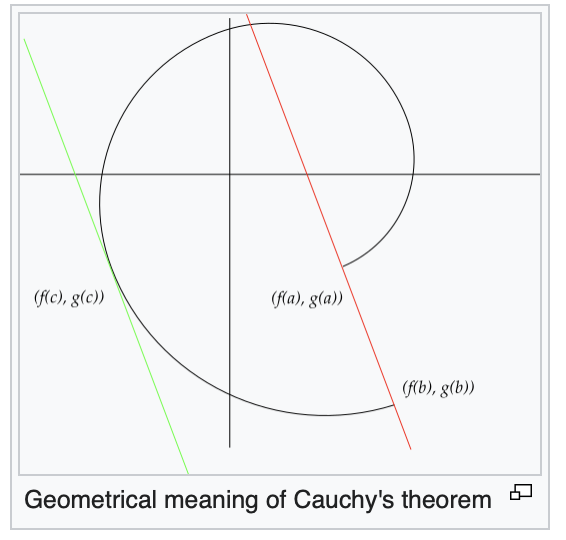
\includegraphics[height=7cm,width=10cm]{CMVT.png}
   \end{minipage}
\end{center}
We now prove \customref{CMVT}{Cauchy's MVT}. 
\end{mdframed}
\begin{theorem}
\label{CMVT}
\textbf{(Cauchy's MVT)} Given a function $f:[a,b]\to \R$ such that  
\begin{enumerate}[label=(\alph*)]
  \item $f,g$ are  differentiable on $(a,b)$
  \item $f,g$ are continuous on $[a,b]$
\end{enumerate}
There exists $x \in (a,b)$ such that 
 \begin{align*}
   \big[f(b)-f(a) \big]g'(x)=\big[g(b)-g(a) \big]f'(x)
\end{align*}
\end{theorem}
\begin{proof}
Define $h$ on  $(a,b)$ by 
\begin{align*}
h(x)\triangleq \big[f(b)-f(a)\big]g'(x)-\big[g(b)-g(a)\big]f'(x)
\end{align*}
We reduced our problem into 
\begin{align*}
  \vi{\text{ finding $x \in (a,b)$ such that } h(x)=0}
\end{align*}
Because $f,g$ are both differentiable on  $(a,b)$, we know there exists an anti-derivative $H$ on  $(a,b)$, which have the form 
\begin{align*}
H(x)=\big[f(b) -f(a)\big]g(x)-\big[g(b)-g(a) \big]f(x)
\end{align*}
\myref{Theorem}{LEoDF} now allow us to reduce the problem into 
\begin{align*}
  \vi{\text{ finding a local extremum of $H$ on  $(a,b)$ }}
\end{align*}
Because $f,g$ are both continuous  on  $[a,b]$, we know $H$ is continuous on $[a,b]$. Then by EVT, we know 
 \begin{align*}
\exists x \in [a,b] , H(x)=\max_{t \in [a,b]}H(t)\text{ and }\exists y \in [a,b], H(y)=\min_{t \in [a,b]}H(t)
\end{align*}
If any of such $x,y$ is in $(a,b)$, we are done. If not, says that $x,y$ both are on end points $a$ or  $b$. Compute that 
\begin{align*}
H(a)=f(b)g(a)-g(b)f(a)=H(b)
\end{align*}
We see $H$ is constant on  $[a,b]$. Then all points in $(a,b)$ are extremums. $\vdone$
\end{proof}
\begin{corollary}
\label{MVT}
\textbf{(Lagrange's MVT)} Given a function $f:[a,b]\rightarrow \R$ such that 
\begin{enumerate}[label=(\alph*)]
  \item $f$ is differentiable on  $(a,b)$ 
  \item $f$ is continuous on  $[a,b]$
\end{enumerate}
Then there exists $x \in (a,b)$ such that 
\begin{align*}
f'(x)=\frac{f(b)-f(a)}{b-a}
\end{align*}
\end{corollary}
\begin{proof}
The proof is done by applying \customref{CMVT}{Cauchy's MVT}, where $g(x)\triangleq x$.
\end{proof}
\begin{mdframed}
There are two hypotheses in Lagrange's MVT 
\begin{enumerate}[label=(\alph*)]
  \item $f$ is differentiable on $(a,b)$ 
  \item $f$ is continuous on $[a,b]$
\end{enumerate}
They are all necessary. The necessity of differentiability on $(a,b)$ is clear as shown by the canonical example using absolute value. The necessity of continuity on $[a,b]$ can be shown by the example 
\begin{align*}
f(x)=\begin{cases}
  1& \text{ if $a<x\leq b$ }\\
  0& \text{ if  }x=a
\end{cases}
\end{align*}
\end{mdframed}
\section{Differentiability Theorem}
\label{Chapter of DT}
\begin{abstract}
This section prove
\begin{enumerate}[label=(\alph*)]
  \item \customref{DiJ}{The matrix representation of derivative for function between Euclidean spaces}
  \item \customref{DT}{Differentiability Theorem}
\end{enumerate}
Note that the proof of \customref{DT}{Differentiability Theorem} use \customref{MVT}{MVT} and the fact \customref{ANoF}{that all norms on $\R^{k}$ are equivalent} where $k=nm$, and utilize the Frobenius norm. 
\end{abstract}
\begin{mdframed}
Given an orthonormal basis  $\set{q_1,\dots ,q_m}$ of $\R^m$ and a function $f:\R^n \rightarrow \R^m$, we let $f_j(x)$ be a real number
\begin{align*}
f_j(x)=f(x)\cdot q_j
\end{align*}
It shall be clear that 
\begin{align*}
f(x)=\sum_{j=1}^m f_j(x)q_j
\end{align*}
which explain why we require $\set{q_1,\dots ,q_m}$ to be orthonormal in the first place. For brevity of the statement of the next theorem (\myref{Theorem}{DiJ}), we introduce another notation. If we are provided a normal basis $\set{e_1,\dots ,e_n}$ of $\R^n$, we denote $\partial_{e_i} f_j(x)$ by $\partial_i f_j(x)$
\end{mdframed}
\begin{theorem}
\label{DiJ}
\textbf{(Derivative is Jacobian)} Suppose  $\alpha =\set{e_1,\dots ,e_n}$ is a basis of $\R^n$, and $\beta =\set{q_1,\dots ,q_m}$ is an orthonormal basis of  $\R^m$. Suppose  $f$ maps an open neighborhood $O$ around $x\inr^n$ to $\R^m$.  Then 
\begin{align*}
  f\text{ is differentiable at }x\implies \begin{cases}
    \partial_{i}f_j(x)\text{ exists for all }i,j\\
    [df_x]_{\alpha }^{\beta }=\begin{bmatrix}
      \partial_1f_1(x)&\cdots & \partial_nf_1(x)\\
      \vdots & \ddots & \vdots\\
      \partial_1f_m(x) & \cdots & \partial_nf_m(x)
    \end{bmatrix}
  \end{cases}
\end{align*}
\end{theorem}
\begin{proof}
Suppose $e_1,\dots ,e_n$ are all normal. Fix $i,j$. We wish to show 
 \begin{align*}
\vi{\partial_i f_j(x) \text{ exists }}
\end{align*}
Because $f$ is differentiable at $x$, by definition of $df_x$, we have
\begin{align*}
\lim_{t\to 0} \frac{\abso{f(x+te_i)-f(x)-df_x(te_i)}}{\abso{te_i}}=0
\end{align*}
Set $R_i:\R\rightarrow \R^m$ by $R_i(t)\triangleq f(x+te_i)-f(x)-df_x(te_i)$. We have 
\begin{align}
\label{Dij1}
  \lim_{t\to 0}\frac{\abso{R_i(t)}}{\abso{t}}=0
\end{align}
Compute
\begin{align*}
f_j(x+te_i)-f_j(x)&=\big(f(x+te_i)-f(x) \big)\cdot q_j\\
&=\big(R_i(t)+df_x(te_i) \big) \cdot q_j\\
&= R_i(t)\cdot q_j+ tdf_x(e_i)\cdot q_j
\end{align*}
This then give us 
\begin{align*}
\frac{f_j(x+te_i)-f_j(x)}{t}=\frac{R_i(t)\cdot q_j}{t}+ df_x(e_i)\cdot q_j
\end{align*}
and 
\begin{align*}
  df_x(e_i)\cdot q_j - \frac{\abso{R_i(t)\cdot q_j}}{\abso{t}} \leq \frac{f_j(x+te_i)-f_j(x)}{t}\leq df_x(e_i)\cdot q_j + \frac{\abso{R_i(t)\cdot q_j}}{\abso{t}}
\end{align*}
By Cauchy-Schwarz Inequality, we now have 
\begin{align*}
  df_x(e_i)\cdot q_j - \frac{\abso{R_i(t)}}{\abso{t}} \leq \frac{f_j(x+te_i)-f_j(x)}{t}\leq df_x(e_i)\cdot q_j + \frac{\abso{R_i(t)}}{\abso{t}}
\end{align*}
Now applying Squeeze Theorem and \myref{Equation}{Dij1}, we have  
\begin{align*}
\partial_i f_j(x)=\lim_{t\to 0} \frac{f_j(x+te_i)-f_j(x)}{t}=df_x(e_i)\cdot q_j \vdone
\end{align*}
Using the fact $\beta $ is orthonormal, we now have 
\begin{align*}
df_x(e_i)=\sum_{j=1}^m \Big(df_x(e_i)\cdot q_j \Big)q_j=\sum_{j=1}^m \partial_if_j(x)q_j
\end{align*}
and suggest the matrix representation. 
\end{proof}
\begin{mdframed}
Note that the converse is not always true. It is possible that a function $f$ has all partial derivatives with respect to a given basis, or even all directions, and yet $f$ is still discontinuous. We have given an example already in \customref{last section}{Directional Derivative and Gradient}. Consider a less trivial one. 
\end{mdframed}

\begin{Example}{\textbf{(Non-differentiable Continuous Funciton with Partial Derivative)}}{}
\begin{align*}
f:\R^2 \rightarrow \R\text{ and }f(x,y)=\begin{cases}
  \frac{x\abso{y}}{\sqrt{x^2+y^2} }& \text{ if $(x,y)\neq 0$ }\\
  0& \text{ if $(x,y)=0$ }
\end{cases}
\end{align*}
We have 
\begin{align*}
\partial_xf(0)=\partial_yf(0)=0
\end{align*}
By \myref{Theorem}{DiJ} (Derivative is Jacobian), if $f$ is differentiable at $0$, then  $df_0$ must be trivial. Yet  
\begin{align*}
\frac{\abso{f(h,h)-f(0)-df_0(h,h)}}{\abso{(h,h)}}=\frac{h }{2\abso{h} }\not\to 0 
\end{align*}
Note that $f$ is continuous at  $0$, by observing 
\begin{align*}
  x^2+y^2- 2\abso{xy}=\big(\abso{x}-\abso{y} \big)^2\geq 0 \implies \frac{x^2+y^2}{2}\geq \abso{xy}
\end{align*}
which implies 
\begin{align*}
\abso{f}\leq \frac{\sqrt{x^2+y^2} }{2}
\end{align*}
\end{Example}
\begin{mdframed}
We now introduce a property of function between normed space that are stronger than differentiability. Given two normed space $\mathcal{X},\mathcal{Y}$, and an open $E\subseteq \mathcal{X}$, we say $f:E\rightarrow \mathcal{Y}$ is \textbf{continuously differentiable } on $\mathcal{Y}$ if the map $D:(E,\norm{\cdot}_\mathcal{X})\rightarrow \Big(BL(\mathcal{X},\mathcal{Y}), \norm{\cdot}_\text{op} \Big)$ defined by 
\begin{align*}
D(x)=df_x
\end{align*}
is continuous. Note that the definition of the term "continuously differentiable" coincide when $\mathcal{X}=\mathcal{Y}=\R$ and $df_x$ is just $h\mapsto f'(x)h$. We now give proof to the  \customref{DT}{Differentiability Theorem}, which links between the continuity of total derivative and the continuity of partial derivatives.
\end{mdframed}
\begin{theorem}
\label{DT}
\textbf{(Differentiability Theorem)} Suppose  $\alpha =\set{e_1,\dots ,e_n}$ is an orthonormal basis of $\R^n$, and $\beta =\set{q_1,\dots ,q_m}$ is an orthonormal basis of  $\R^m$. Suppose  $f$ maps an open set $E\subseteq\R^n$ to $\R^m$.  Then  
\begin{align*}
f\text{ is continuously differentiable on $E$ }\iff \partial_if_j\text{ exists and is continuous on $E$ for all $i,j$ }
\end{align*}
\end{theorem}
\begin{proof}
$(\longrightarrow)$\\

Fix $i,j$. Because $f$ is differentiable on $E$, we know  $\partial_i f_j$ exists on $E$ by \myref{Theorem}{DiJ}. Fix $x \in E$. We only have to show 
\begin{align*}
  \vi{\partial_i f_j\text{ is continuous at $x$ }}
\end{align*}
Fix $\epsilon $. We wish 
\begin{align*}
\vi{\text{ to find }\delta\text{ such that } \abso{\partial_i f_j(y)-\partial_i f_j(x)}\leq \epsilon \text{ for all $\abso{y-x}<\delta$ }}
\end{align*}
Because $f$ is continuously differentaible at $x$, we know there exists  $\delta$ such that 
\begin{align*}
\norm{df_y-df_x}_\text{op}< \epsilon \text{ for all $\abso{y-x}\leq \delta$ }
\end{align*}
We claim 
\begin{align*}
\vi{\text{ such $\delta$ suffices }}
\end{align*}
By the \customref{DiJ}{the matrix representation}, we know
\begin{align*}
\partial_i f_j(y)-\partial_i f_j(x)=(df_y-df_x)e_i \cdot q_j
\end{align*}
Then by Cauchy-Inequality, we have 
\begin{align*}
  \abso{\partial_i f_j(y)-\partial_if_j(x)}&\leq \abso{(df_y-df_x)e_i}\\
  &\leq \norm{df_y-df_x}_\text{op}<\epsilon \vdone
\end{align*}

$(\longleftarrow)$\\

We first show 
\begin{align*}
\vi{f\text{ is differentiable on $E$ }}
\end{align*}
We first prove 
\begin{align*}
\olive{\forall j\in \set{1,\dots, m}, f_j:\R^n\rightarrow \R\text{ is differentiable on $E$ }\implies f\text{ is differentiable on $E$ }}
\end{align*}
Fix $x\in E$. We wish to prove 
\begin{align*}
\olive{\text{ $f$ is differentiable at $x$ }}
\end{align*}
Define $A:E\rightarrow \R^m$ by 
\begin{align*}
A(h)\triangleq \sum_{j=1}^m  (df_j)_x (h)q_j
\end{align*}
We claim 
\begin{align*}
\olive{A\text{ suffices to be the $df_x$ }}
\end{align*}
Using the fact $q_j$ are orthonormal, we have
\begin{align*}
f(x+h)-f(x)-A(h)=\sum_{j=1}^m \big(f_j(x+h)-f_j(x)-(df_j)_x(h)  \big)q_j
\end{align*}
This give us 
\begin{align*}
\lim_{h\to 0} \frac{\abso{f(x+h)-f(x)-A(h)}}{\abso{h}}&=\lim_{h\to 0} \frac{\abso{\sum_{j=1}^m \big(f_j(x+h)-f_j(x)-(df_j)_x (h) \big)q_j}}{\abso{h}}\\
&\leq \lim_{h\to 0} \frac{\sum_{j=1}^m \abso{f_j(x+h)-f_j(x)-(df_j)_x(h)}}{\abso{h}}=0 \odone
\end{align*}
Fix $j \in \set{1,\dots ,m}$. We can now reduce the problem into 
\begin{align*}
  \vi{f_j:\R^n\rightarrow \R\text{ is differentiable on $E$ }}
\end{align*}
Fix $x \in E$. We wish to prove 
\begin{align*}
\vi{f_j\text{ is differentiable at $x$ }}
\end{align*}
Express $h=\sum_{i=1}^n h_ie_i$. Define $B:E\rightarrow \R$ by
\begin{align*}
B(h)=\sum_{i=1}^n \partial_i f_j(x)h_i
\end{align*}
We claim 
\begin{align*}
\vi{B\text{ suffices to be $(df_j)_x$ }}
\end{align*}
By continuity of each $\partial_i f_j$ on $E$, we can let  $\delta$ satisfy 
\begin{align*}
\abso{\partial_i f_j(y)-\partial_i f_j(x)}<  \frac{\epsilon }{n}  \text{ for all $y\in B_\delta(x)$  }
\end{align*}
We claim 
\begin{align*}
  \vi{\frac{\abso{f_j(y)-f_j(x)-B(y-x)}}{\abso{y-x}}\leq \epsilon \text{ for all }y \in B_\delta (x)}
\end{align*}
Express $y-x=\sum_{k=1}^n h_ke_k$. Define $v_0,\dots,v_n\inr^n$ by
\begin{align*}
v_0\triangleq 0\text{ and }v_k\triangleq \sum_{i=1}^k h_ie_i\text{ for all $k\in \set{1,\dots ,n}$ }
\end{align*}
Now observe
\begin{align*}
\frac{\abso{f_j(y)-f_j(x)-B(y-x)}}{\abso{y-x}}&=\frac{\abso{f_j(x+v_n)-f_j(x)-B(\sum_{k=1}^n h_ke_k)}}{\abso{y-x}}\\
&=\frac{\abso{\big(\sum_{k=1}^nf_j(x+v_k)-f_j(x+v_{k-1}) \big)- \sum_{k=1}^n \partial_k f_j(x)h_k   }}{\abso{y-x}}\\
&=\frac{\abso{\sum_{k=1}^n f_j(x+v_k)-f_j(x+v_{k-1})-\partial_k f_j(x)h_k}}{\abso{y-x}}\\
&=\frac{\abso{\sum_{k=1}^n f_j(x+v_{k-1}+h_ke_k)-f_j(x+v_{k-1})-\partial_k f_j(x)h_k}}{\abso{y-x}}\\
(\text{ For some $e_k\in (0,1)$ by \customref{MVT}{MVT}})\hspace{0.5cm}&=\frac{\abso{\sum_{k=1}^n \partial_k f_j(x+v_{k-1}+t_ke_k)h_k-\partial_k f_j(x)h_k}}{\abso{y-x}}\\
&\leq \frac{\sum_{k=1}^n \abso{\big(\partial_k f_j(x+v_{k-1}+t_ke_k)-\partial_k f_j(x) \big)h_k}}{\abso{y-x}}\\
&< \frac{\sum_{k=1}^n \frac{\epsilon }{n} \abso{h_k}}{\abso{y-x}}\leq \epsilon \vdone
\end{align*}
We now prove
\begin{align*}
\blue{f\text{ is continuously differentiable on $E$ }}
\end{align*}
Fix $\epsilon $ and $x\in E$. We are required 
\begin{align*}
\blue{\text{ to find $\delta$ such that $\norm{df_y-df_x}_\text{op}\leq \epsilon $ for all $y\in B_\delta (x)$ }}
\end{align*}
Note that one can define a norm $\norm{\cdot}_F$ called "Forbenius Norm" on $BL(\R^n,\R^n)$ by 
\begin{align*}
\norm{A}_F\triangleq \sqrt{\sum_{i=1}^n \sum_{j=1}^n a_{i,j}^2}  \text{ where }[A]_\alpha ^\beta = \begin{bmatrix}
  a_{1,1}& \cdots & a_{n,1}\\
  \vdots & \ddots & \vdots \\
  a_{1,n} & \cdots & a_{n,n}  
\end{bmatrix}
\end{align*}
Because \customref{ANoF}{all norms on finite-dimensional real vector spaces are equivalent}, we know there exists $M$ such that for all $x\in E$, we have 
\begin{align*}
\norm{df_x}_\text{op}\leq  M\norm{df_x}_F
\end{align*}
Because the partial derivatives are all continuous by definition, we can let $\delta$ satisfy 
\begin{align*}
  \big(\partial_i f_j(x+h)\big)^2-\big(\partial_i f_j(x)\big)^2< \frac{\epsilon^2 }{M^2n^2}\text{ for all $h \in B_\delta (0)$ }
\end{align*}
We claim 
\begin{align*}
\blue{\text{ such }\delta\text{ suffices }}
\end{align*}
Let $\abso{y-x}<\delta$. We see 
\begin{align*}
\norm{df_y-df_x}_\text{op}\leq M\norm{df_y -df_x}_F< M \sqrt{\sum_{i=1}^n \sum_{j=1}^n\frac{\epsilon^2 }{M^2n^2}}=\epsilon \bdone
\end{align*}












\end{proof}

\section{Product Rule and Chain Rule}
\begin{abstract}
This short section prove \customref{Product Rule}{Product rule in the setting of gradient of real-valued function} and  \customref{CR}{Chain rule for functions between normed spaces}, which is heavily used in \customref{Smoothness}{next section on smooth function} and \customref{Differential Geometry}{Differential Geometry}. 
\end{abstract}
\begin{mdframed}
Although distinct versions of product rule exists in the context of vector calculus, here we prove the almost most simple kind.  
\end{mdframed}
\begin{theorem}
\label{Product Rule}
\textbf{(Product Rule)} Given two function  $f,g:\R^d\rightarrow \R$ differentiable at $x$, we have 
\begin{align*}
\nabla (fg)(x)= g(x) \nabla f(x)+ f(x)\nabla g(x)
\end{align*}
\end{theorem}
\begin{proof}
Note that 
\begin{align*}
  \lim_{h\to 0}f(x+h)\Big[\frac{g(x+h)-g(x)-\nabla g(x)\cdot h}{\abso{h}} \Big]&= 0 \\
  \text{ and }\lim_{h\to 0} g(x)\Big[ \frac{f(x+h)-f(x)-\nabla f(x)\cdot h}{\abso{h}}\Big]=0
\end{align*}
Adding these two equations together, we have 
\begin{align*}
\lim_{h\to 0}  \frac{f(x+h)g(x+h)-f(x)g(x)-[g(x)\nabla f(x)+f(x)\nabla g(x)]\cdot h}{\abso{h}}=0
\end{align*}
\end{proof}
\begin{mdframed}
We now prove the Chain Rule for function between normed space. 
\end{mdframed}
\begin{theorem}
\label{CR}
\textbf{(Chain Rule)} Given three normed space $\mathcal{X},\mathcal{Y},\mathcal{Z}$, a point $x \in \mathcal{X}$, a function $g$ that map an open set $U\subseteq \mathcal{Y}$ containing $f(x)$ into $\mathcal{Z}$, a function $f$ that map an open-neighborhood around $x$ into $U$ such that 
\begin{enumerate}[label=(\alph*)]
  \item $f$ is differentiable at $x$
   \item $g$ is differentiable at $f(x)$
\end{enumerate}
we have 
\begin{align*}
d(g\circ f)_x=dg_{f(x)}\circ df_{x}
\end{align*}
\end{theorem}
\begin{proof}
For brevity, we use $F\triangleq g\circ f$. We wish to prove 
\begin{align*}
\vi{\lim_{h\to 0}\frac{\norm{F(x+h)-F(x)-dg_{f(x)}df_x(h)}_\mathcal{Z}}{\norm{h}_\mathcal{X}}=0}
\end{align*}
Fix $k\triangleq f(x+h)-f(x)$. Observe 
\begin{align*}
 F(x+h)-F(x)-dg_{f(x)}df_x(h)=\Big(g\big(f(x)+k\big)-g\big(f(x)\big)- dg_{f(x)}(k) \Big) + dg_{f(x)}\big(k-df_x(h)\big)
\end{align*}
This now implies 
\begin{align*}
&\frac{\norm{F(x+h)-F(x)-dg_{f(x)}df_x(h)}_\mathcal{Z}}{\norm{h}_\mathcal{X}}\text{ is smaller than }
\end{align*}
\begin{align*}
\frac{\norm{g\big(f(x)+k\big)-g\big(f(x)\big)- dg_{f(x)}(k) }_Z+ \norm{dg_{f(x)}\big(k-df_x(h)\big)}_\mathcal{Z}}{\norm{h}_\mathcal{X}} 
\end{align*}
This let us reduce the problem into proving 
\begin{align*}
  &\olive{ \lim_{h\to 0}\frac{\norm{g\big(f(x)+k\big)-g\big(f(x)\big)- dg_{f(x)}(k) }_Z }{\norm{h}_\mathcal{X}} =0}\\
  \text{ and }&\blue{\lim_{h\to 0} \frac{\norm{dg_{f(x)}\big(k-df_x(h) \big)}_\mathcal{Z}}{\norm{h}_\mathcal{X}}=0}
\end{align*}
We first prove 
\begin{align*}
\olive{ \lim_{h\to 0}\frac{\norm{g\big(f(x)+k\big)-g\big(f(x)\big)- dg_{f(x)}(k) }_Z }{\norm{h}_\mathcal{X}} =0}
\end{align*}
Note that if $\norm{k}_\mathcal{Y}=0$, we have 
\begin{align*}
\frac{\norm{g\big(f(x)+k\big)-g\big(f(x)\big)- dg_{f(x)}(k) }_Z }{\norm{h}_\mathcal{X}} =0
\end{align*}
Now, observe that 
\begin{align*}
\frac{\norm{g\big(f(x)+k\big)-g\big(f(x)\big)- dg_{f(x)}(k) }_Z }{\norm{h}_\mathcal{X}} = \frac{\norm{g\big(f(x)+k\big)-g\big(f(x)\big)- dg_{f(x)}(k) }_Z }{\norm{k}_\mathcal{Y}}\cdot \frac{\norm{k}_\mathcal{Y}}{\norm{h}_\mathcal{X}} 
\end{align*}
Because $h \to 0 \implies k\to 0$, we can now reduce the problem into proving 
\begin{align*}
\olive{\limsup_{h\to 0} \frac{\norm{k}_\mathcal{Y}}{\norm{h}_\mathcal{X}}\text{ exists }}
\end{align*}
Observe 
\begin{align*}
\frac{\norm{k}_\mathcal{Y}}{\norm{h}_\mathcal{X}}&= \frac{\norm{f(x+h)-f(x)-df_x(h)+df_x(h)}_\mathcal{X}}{\norm{h}_\mathcal{X}}\\
&\leq \frac{\norm{f(x+h)-f(x)-df_x(h)}_\mathcal{Y}}{\norm{h}_\mathcal{X}}+\frac{\norm{df_x(h)}_\mathcal{Y}}{\norm{h}_\mathcal{X}}\\
&\leq \frac{\norm{f(x+h)-f(x)-df_x(h)}_\mathcal{Y}}{\norm{h}_\mathcal{X}} + \norm{df_x}_\text{op} \odone
\end{align*}
We now prove 
\begin{align*}
\blue{\lim_{h\to 0} \frac{\norm{dg_{f(x)}\big(k-df_x(h) \big)}_\mathcal{Z}}{\norm{h}_\mathcal{X}}=0}
\end{align*}
Note that if $f(x+h)-f(x)-df_x(h)=0$, then $\norm{dg_{f(x)}\big(k-df_x(h) \big)}_\mathcal{Z}=0$. Now, observe 
\begin{align*}
\frac{\norm{dg_{f(x)}\big(k-df_x(h) \big)}_\mathcal{Z}}{\norm{h}_\mathcal{X}}&= \frac{\norm{dg_{f(x)}\big(f(x+h)-f(x)-df_x(h) \big)}_\mathcal{Z}}{\norm{f(x+h)-f(x)-df_x(h)}_\mathcal{Y}}\cdot \frac{\norm{f(x+h)-f(x)-df_x(h)}_\mathcal{Y}}{\norm{h}_\mathcal{X}}\\
&\leq \norm{dg_{f(x)}}_\text{op}\cdot \frac{\norm{f(x+h)-f(x)-df_x(h)}_\mathcal{Y}}{\norm{h}_\mathcal{X}}\to 0 \bdone
\end{align*}
\end{proof}
\section{Smoothness}
\label{Smoothness}
\begin{abstract}
This is a short section introducing the idea of smooth functions between Euclidean spaces, which heavily rely on \customref{CR}{Chain Rule}. One should note that our \textbf{notation} $\partial _{21}f$ here means $\partial_2 (\partial_1 f)$.  
\end{abstract}
\begin{theorem}
\label{SoMPD}
\textbf{(Structure of Mixed Partial Derivative)} Given an open set $E\subseteq \R^2$, a point $p\in  E$, a basis $\set{e_1,e_2}$ of $\R^2$ and a function $f:E\rightarrow \R$ such that 
\begin{enumerate}[label=(\alph*)]
  \item $\partial_1 f$ exists on $E$
   \item $\partial_2 f$ exists on $E$
     \item $\partial_{21} f$ exists on $E$ and is continuous at $p$
\end{enumerate}
We have
\begin{align*}
\partial_{12} f(p)=\partial_{21}f(p)
\end{align*}
\end{theorem}
\begin{proof}
Express elements of $E$ in the basis $\set{e_1,e_2}$, and express $p=(a,b)$. We are required to prove 
\begin{align*}
  \vi{\lim_{h\to 0}\frac{\partial_2f(a+h,b)-\partial_2 f(a,b)}{h}=\partial_{21}f(a,b)}
\end{align*}
Let $D\triangleq \set{q-(a,b)\inr^2:q\in E\setminus \set{p}}$ and define $\Delta(h,k):D\rightarrow \R$ by 
\begin{align*}
\Delta(h,k)\triangleq f(a+h,b+k)-f(a,b+k)-f(a+h,b)+f(a,b)
\end{align*}
Note that because $\partial_2f$ exists on $E$, for all $h\neq 0$, we have 
 \begin{align*}
\lim_{k\to 0} \frac{\Delta (h,k)}{hk}=\frac{\partial_2 f(a+h,b)-\partial_2 f(a,b)}{h}
\end{align*}
This let us reduce the problem into proving 
\begin{align*}
  \vi{\lim_{h\to 0}\lim_{k\to 0} \frac{\Delta (h,k)}{hk}=\partial_{21}f(a,b)}
\end{align*}
We first show 
\label{oea}

\begin{center}
   \begin{minipage}{0.9\linewidth}  
     \olive{For all $(h,k)\in D:hk\neq 0$, $\frac{\Delta (h,k)}{hk}=\partial_{21}f(x,y)$ for some $(x,y)\in D:\abso{x-a}<h\text{ and }\abso{y-b}<k$}. \label{oea}
   \end{minipage}
\end{center}
Fix $(h,k)\in D: hk\neq 0$. Define $u:(b-\epsilon ,b+\epsilon )\rightarrow \R$ by 
\begin{align*}
u(t)\triangleq f(t,b+k)-f(t,b)
\end{align*}
\customref{CR}{Chain Rule} allow us to compute   
\begin{align*}
u'(t)=\partial_1 f(t,b+k)-\partial_1 f(t,b)
\end{align*}
We then can deduce
\begin{align*}
\Delta (h,k)&=u(a+h)-u(a)\\
            &=hu'(x)\text{ for some $x\in (a,a+h)$ by \customref{MVT}{MVT}}\\
&=h\big(\partial_1 f(x,b+k)-\partial_1 f(x,b) \big)
\end{align*}
Now, because $\partial_{21}f$ exists on $E$, we can deduce
\begin{align*}
\Delta (h,k)&=h(\partial_1 f(x,b+k)-\partial_1 f(x,b))\\
&=hk\partial_{21}f(x,y)\text{ for some $y\in (b,b+k)$ by \customref{MVT}{MVT}}\odone
\end{align*}
Fix $\epsilon $. We wish 
\begin{align*}
  \vi{\text{ to find some $\delta$ such that for all }h:0<\abso{h}<\delta, \abso{\lim_{k\to 0}\frac{\Delta (h,k)}{hk}-\partial_{21}f(x,y)}\leq \epsilon }
\end{align*}
Because $\partial_{21}f$ is continuous at $p$, by \olive{olive lemma}, we know there exists $\delta$ such that  
\begin{align*}
  \abso{\frac{\Delta ( h,k)}{hk}-\partial_{21}f(a,b)}<\frac{\epsilon }{2}\text{ for all }h,k \in (-\delta,\delta)\setminus \set{0}
\end{align*}
We claim 
\begin{align*}
\vi{\text{ such }\delta\text{ works }}
\end{align*}
Fix $h:0<\abso{h}<\delta$. Note that $\lim_{k\to 0}\frac{\Delta (h,k)}{hk}=\frac{\partial_2 f(a+h,b)-\partial_2 f(a,b)}{h}$ exists, so we can find small enough $k'$ such that
\begin{align*}
  0<\abso{k'}<\delta \text{ and } \abso{\lim_{k\to 0} \frac{\Delta (h,k)}{hk}- \frac{\Delta (h,k')}{hk'}}<\frac{\epsilon}{2}
\end{align*}
Now observe 
\begin{align*}
\abso{\lim_{k\to 0}\frac{\Delta (h,k)}{hk}-\partial_{21}f(x,y)}\leq \abso{\lim_{k\to 0}\frac{\Delta (h,k)}{hk}-\frac{\Delta (h,k')}{hk'}}+ \abso{\frac{\Delta (h,k')}{hk'}-\partial_{21}f(a,b)}\leq \epsilon \vdone
\end{align*}





\end{proof}
\begin{corollary}
\textbf{(Clairaut's Theorem on equality of mixed partial)} Given a basis $\set{e_1,\dots ,e_n}$ of $\R^n$, an open set $E\subseteq \R^n$, a function $f:E\rightarrow \R$ such that 
\begin{align*}
\partial_{ij}f\text{ exist and is continuous on }E\text{ for all }i,j \in \set{1,\dots ,n}
\end{align*}
We have  
\begin{align*}
\partial_{ij}f=\partial_{ji}f\text{ on $E$ for all }i,j\in \set{1,\dots ,n}
\end{align*}
\end{corollary}
\begin{mdframed}
Given a function $f:E\subseteq \R^n\rightarrow \R$, we now see that, by \customref{DT}{Differentiability Theorem}, if $\partial_x f,\partial_{xy}f$ exist on $E$ and the latter is continuous on $E$, then  $f$ is continuously differentiable on $E$.    
\end{mdframed}
\begin{Example}{\textbf{(A $C^1$ but not $C^2$ function)}}{}
\begin{align*}
  f(x,y)\triangleq \begin{cases}
   \frac{xy(x^2-y^2)}{x^2+y^2}& \text{ if $(x,y)\neq 0$ }\\
   0& \text{ if $(x,y)=0$ }
  \end{cases}
\end{align*}
All second order partial derivatives exist, yet $f_{xy},f_{yx}$ does not commute at $0$. 
\end{Example}
\begin{mdframed}
Now, if we define a function $f:U\subseteq \R^n\rightarrow \R^m$ on some open subset $U$ to be \textbf{smooth} if for all $j\in \set{1,\dots ,m}$, all partial derivatives of $f$ exists, we then see that the partial derivatives of smooth function always commute. Notably, one can check that if $f:U\subseteq \R^n\rightarrow \R^m$, and $g:V\subseteq \R^m\rightarrow \R^d$ are both smooth and $f(U)\subseteq V$, then $g\circ f:U\rightarrow \R^d$ is also smooth, using long tedious induction with \customref{Product Rule}{Product rule} and \customref{CR}{Chain rule}. 
\end{mdframed}
\section{Complex Differentiation}
\begin{abstract}
This is a short section introducing the idea of complex-differentiable function and prove some of their basic properties, i.e., \customref{Cauchy Riemann Criteria}{Cauchy Riemann Criteria} and \customref{Product and Quotient Rule for Holomorphic Function}{Product and Quotient Rule for Complex-differentiable Function}. 
\end{abstract}
\begin{mdframed}
Given a complex-valued function $f$ defined on some open subset of  $\C$ containing  $z$, we say  $f$ is \textbf{complex-differentiable at $z$} if there exists some complex number denoted by $f'(z)$ such that 
\begin{align*}
\frac{f(z+h)-f(z)-f'(z)h}{h}\to 0\text{ as }h\to 0;h\inc
\end{align*}
Immediately, one can see that a complex-differentiable function when viewed as a function between $\R^2$ is differentiable with derivative 
\begin{align}
\label{cd}
  \begin{bmatrix}
    a & -b \\
    b & a
  \end{bmatrix}\text{ where }f'(z)=a+b i
\end{align}
With the form of derivative in mind, one may conjecture that complex-differentiable is a 'stricter' condition than merely differentiable when regarded as function between $\R^2$. This is exactly true. Consider the following example.
\end{mdframed}
\begin{Example}{\textbf{(A non complex-differentiable function)}}{}
\begin{align*}
f(z)\triangleq \overline{z}
\end{align*}
This is a linear function with matrix representation 
\begin{align*}
\begin{bmatrix}
  1&0 \\
  0& -1
\end{bmatrix}
\end{align*}
which doesn't fit the necessary form in \myref{Equation}{cd}.
\end{Example}
\begin{theorem}
\label{Cauchy Riemann Criteria}
\textbf{(Cauchy Riemann Criteria)} Given a complex-valued function $f$ defined on some open subset $U$ of $\C$ containing  $z$, if we write 
 \begin{align*}
f(x+yi)=u(x,y)+iv(x,y)
\end{align*}
where $u,v:U\rightarrow \R$, then the following two statements are equivalent.
\begin{enumerate}[label=(\alph*)]
  \item $f$ is complex differentiable at  $z$. 
  \item $u,v$ are differentiable at  $z$ when $U$ is viewed as subsets of $\R^2$ and 
\begin{align*}
    \frac{\partial u}{\partial x}=\frac{\partial v}{\partial y}\text{ and }\frac{\partial u}{\partial y}=\frac{-\partial v}{\partial x}\text{ at }z
\end{align*}
\end{enumerate}
\end{theorem}
\begin{proof}
(a) to (b) is an immediate result of \customref{CR}{Chain Rule} and \customref{DiJ}{matrix representation of $f'(z)$}. Suppose  (b) is true. Let $h=h_1+ih_2$ and $z=x+yi$. Because $u,v$ are differentiable at  $(x,y)$, by the \customref{DiJ}{matrix representation of derivative}, we have 
\begin{align*}
\frac{f(z+h)-f(z)}{h}&= \frac{u(x+h_1,y+h_2)-u(x,y)}{h_1+ih_2}+ i \frac{v(x+h_1,y+h_2)-v(x,y)}{h_1+ih_2}\\
&=\frac{h_1u_x+h_2u_y+ih_1v_x+ih_2v_y+o(\abso{h})}{h_1+ih_2}\\
&=\frac{(h_1+ih_2)u_x+i(h_1+ih_2)v_x+o(\abso{h})}{h_1+ih_2}\\
&=u_x+iv_x+\frac{o(\abso{h})}{h_1+ih_2}\to u_x+iv_x
\end{align*}
\end{proof}
\begin{theorem}
\label{Product and Quotient Rule for Holomorphic Function}
\textbf{(Product and Quotient Rule for Complex-differentiable  Function)} Given two function $f,g$ complex-differentiable at  $z$, we have 
 \begin{align*}
   (fg)'(z)= f'(z)g(z)+f(z)g'(z)
\end{align*}
and if $g(z)\neq 0$, we also have 
\begin{align*}
\Big(\frac{f}{g}\Big)'(z)=\frac{f'(z)g(z)-f(z)g'(z)}{(g(z))^2}
\end{align*}
\end{theorem}
\begin{proof}
Observe
\begin{align*}
  &\frac{f(z+h)g(z+h)-f(z)g(z)}{h}\\
  =&f(z+h)\Big[\frac{g(z+h)-g(z)}{h} \Big] +g(z) \Big[\frac{f(z+h)-f(z)}{h} \Big]\to f'(z)g(z)+f(z)g'(z)
\end{align*}
and 
\begin{align*}
\frac{\frac{f(z+h)}{g(z+h)}-\frac{f(z)}{g(z)}}{h}&= \frac{f(z+h)g(z)-f(z)g(z+h)}{g(z+h)g(z)h}\\
&=\frac{1}{g(z+h)g(z)}\Big[ g(z)\Big(\frac{f(z+h)-f(z)}{h}\Big)-f(z)\Big(\frac{g(z+h)-g(z)}{h} \Big) \Big]\\
&\to \frac{f'(z)g(z)-f(z)g'(z)}{(g(z))^2}
\end{align*}
\end{proof}
\section{Uniform Convergence and Differentiation}
\begin{abstract}
This is a section discussing the relationship between uniform convergence and differentiation, which heavily rely on the usage of \customref{MVT}{MVT}, and is used to prove \customref{AfaS}{Analytic function is smooth}. 
\end{abstract}
\begin{mdframed}
Before stating \myref{Theorem}{UCaD}, let's see three examples why we don't (can't) use the hypothesis: $f_n \to f$ uniformly in our statement of \myref{Theorem}{UCaD} 
\begin{Example}{\textbf{(Differentiable functions are NOT closed under uniform convergence)}}{}
\begin{align*}
X=[-1,1]\text{ and }f(x)=\abso{x}
\end{align*}
By \customref{WaT}{Weierstrass approximation Theorem}, there is a sequence of polynomials (differentiable) that uniformly converge to $f$, which is not differentiable at  $0$. 
\end{Example}
\begin{Example}{\textbf{(Derivative won't necessarily converge to the right place)}}{}
\begin{align*}
X=\R \text{ and }f_n(x)=\frac{\sin nx}{\sqrt{n} }
\end{align*}
Compute 
\begin{align*}
f'(x)=0 \text{ and }f'_n(x)=\sqrt{n} \cos nx
\end{align*}
\end{Example}
\begin{Example}{\textbf{(Derivative won't necessarily converge to the right place)}}{}
\begin{align*}
X=\R \text{ and }f_n(x)=\frac{x}{1+nx^2}
\end{align*}
Compute 
\begin{align*}
f=\tilde{0} \text{ and }f'_n(0)=1
\end{align*}
\end{Example}
Informally speaking, these examples together with the fact \customref{RIFac}{Riemann integral are closed under uniform convergence} should give you some ideas that differentiation and integration although are operations inverse to each other, are NOT symmetric. There is a certain hierarchy on continuous functions on a fixed compact interval. Thus, we have the next Theorem in its form. Note that in application, the next Theorem only require us to prove $f'_n$ uniformly converge, and doesn't require us to prove to where does it converge. 
\end{mdframed}
\begin{theorem}
\label{UCaD}
\textbf{(Uniform Convergence and Differentiation)} Given a bounded interval $[a,b]$ and some sequence of function $f_n:[a,b]\rightarrow \R$ such that 
\begin{enumerate}[label=(\alph*)]
  \item $f'_n$ uniformly converge on  $(a,b)$
  \item $f_n$ are continuous on  $[a,b]$
  \item $f_n(x_0)\to L$ for some $x_0 \in [a,b]$
\end{enumerate}
Then 
\begin{enumerate}[label=(\alph*)]
  \item $f_n$ uniformly converge on  $[a,b]$ 
  \item and
\begin{align*}
\Big(\lim_{n\to \infty}f_n \Big)'(x_0)=\lim_{n\to \infty}f_n'(x_0)\text{ on $(a,b)$ }
\end{align*}
\end{enumerate}
\end{theorem}
\begin{proof}
We first prove 
\begin{align}
\label{fnun}
\vi{f_n\text{ uniformly converge on $[a,b]$}}
\end{align}
Fix $\epsilon $. We wish  
\begin{align*}
  \vi{\text{ to find $N$ such that $\norm{f_n-f_m}_\infty \leq \epsilon $ for all $n,m>N$}}
\end{align*}
Because $f_n(x_0)$ converge, and $f'_n$ uniformly converge, we know there exists $N$ such that 
 \begin{align}
\label{UCD1}
\begin{cases}
 \abso{f_n(x_0)-f_m(x_0)}<\frac{\epsilon}{2} \\
\norm{f_n'-f_m'}_\infty <\frac{\epsilon }{2(b-a)}
\end{cases}\text{ for all $n,m>N$ }
\end{align}
We claim 
\begin{align*}
\vi{\text{ such $N$ works }}
\end{align*}
Fix $x \in [a,b]$ and $n,m>N$. We first show
\begin{align*}
\olive{\abso{\big(f_n-f_m\big)(x)-\big(f_n-f_m \big)(x_0)}\leq \frac{\epsilon}{2}}
\end{align*}
Because $(f_n-f_m)'=f_n'-f_m'$, by \customref{MVT}{MVT} and \myref{Equation}{UCD1}, we can deduce 
\begin{align*}
 \abso{\big(f_n-f_m\big)(x)-\big(f_n-f_m \big)(x_0)}&=\Big|\big[(f_n-f_m)'(t)\big](x-x_0)\Big|\text{ for some $t$ between $x,x_0$ }\\
 &< \frac{\epsilon}{2(b-a)}\cdot \abso{x-x_0}\\
 &\leq \frac{\epsilon }{2(b-a)}\cdot (b-a)=\frac{\epsilon}{2}\hspace{0.3cm}\big(\because x,x_0  \in [a,b]\big)\odone
\end{align*}
Now, by \myref{Equation}{UCD1}, we have 
\begin{align*}
  \abso{\big(f_n-f_m \big)(x)}&\leq \abso{\big(f_n-f_m \big)(x)-\big(f_n-f_m \big)(x_0)}+\abso{\big(f_n-f_m \big)(x_0)}\\
&<\frac{\epsilon}{2}+\frac{\epsilon}{2}=\epsilon \vdone
\end{align*}
Let $f:[a,b]\rightarrow \R$ be the limit of $f_n$. It remains to prove
\begin{align}
\label{UCAC2}
\blue{f'(x)=\lim_{n\to \infty}f_n'(x)\text{ on }(a,b)}
\end{align}
Fix $x\in (a,b)$ and define $\phi ,\phi_n:[a,b]\setminus x\rightarrow \R$ by 
\begin{align*}
\phi (t)\triangleq \frac{f(t)-f(x)}{t-x}\text{ and }\phi_n(t)\triangleq \frac{f_n(t)-f_n(x)}{t-x}
\end{align*}
It is clear that $\phi_n\to \phi$ pointwise on $[a,b]\setminus x$. We now show 
\begin{align*}
\olive{\phi_n\to \phi\text{ uniformly on }[a,b]\setminus x}
\end{align*}
Fix $\epsilon $. We have
\begin{align*}
  \olive{\text{ to find $N$ such that  $\abso{\phi_n(t)-\phi _m(t)}\leq \epsilon $ for all $n,m>N$ and  $t\in [a,b]\setminus x$ }}
\end{align*}
Because $f_n'$ uniformly converge on  $(a,b)$, we know there exists $N$ such that 
 \begin{align}
\label{CUaC1}
\norm{f_n'-f_m'}_\infty\leq \epsilon \text{ for all $n,m>N$ }
\end{align}
We claim 
\begin{align*}
\olive{\text{ such }N\text{ works }}
\end{align*}
Fix $n,m>N$ and $t \in [a,b]\setminus x$. We wish to prove 
\begin{align*}
\olive{\abso{\phi_n(t)-\phi_m(t)}\leq \epsilon }
\end{align*}
Because $(f_n-f_m)'=f_n'-f'_m$, by \customref{MVT}{MVT} and \myref{Equation}{CUaC1}, we can deduce 
\begin{align*}
  \abso{\phi_n(t)-\phi_m(t)}&\leq \abso{\frac{f_n(t)-f_n(x)}{t-x}-\frac{f_m(t)-f_m(x)}{t-x}}\\
                            &=\abso{\frac{\big(f_n-f_m\big)(t)-\big(f_n-f_m\big)(x)}{t-x}}\\
 &=\abso{\big(f'_n-f'_m\big)(t_0)}\text{ for some $t_0$ between $t,x$  }\\
&\leq \epsilon \odone
\end{align*}
Note that 
\begin{align*}
\lim_{n\to \infty}\lim_{t\to x}\phi_n(t)=\lim_{n\to \infty}f'(x)\text{ exists }
\end{align*}
We can now \customref{COLO}{exchange the limit} and see that the derivative of $f$ at $x$ exists. 
\begin{align*}
f'(x)=\lim_{t\to x}\phi (t)&=\lim_{t\to x}\lim_{n\to \infty}\phi_n(t)\\
&=\lim_{n\to \infty}\lim_{t\to x}\phi_n(t)=\lim_{n\to \infty}f'_n(x) \bdone
\end{align*}
\end{proof}
\begin{theorem}
\label{UCaH}
\textbf{(Uniform Convergence and Holomorphic)} Given a real number $r$ and some sequence of function $f_n:\overline{D_r(z_0)}\rightarrow \C$ such that 
\begin{enumerate}[label=(\alph*)]
  \item $f'_n$ uniformly converge on  $D_r(z_0)$
  \item $f_n$ are continuous on  $\overline{D_r(z_0)}$
  \item $f_n(v)\to L$ for some $v \in \overline{D_r(z_0)}$
\end{enumerate}
Then 
\begin{enumerate}[label=(\alph*)]
  \item $f_n$ uniformly converge on  $\overline{D_r(z_0)}$ 
  \item and
\begin{align*}
\Big(\lim_{n\to \infty}f_n \Big)'(z)=\lim_{n\to \infty}f_n'(z)\text{ on $D_r(z_0)$ }
\end{align*}
\end{enumerate}
\end{theorem}
\begin{proof}
We first prove 
\begin{align}
\label{fnun}
\vi{f_n\text{ uniformly converge on $\overline{D_r(z_0)}$}}
\end{align}
Fix $\epsilon $. We wish  
\begin{align*}
  \vi{\text{ to find $N$ such that $\norm{f_n-f_m}_\infty \leq \epsilon $ for all $n,m>N$}}
\end{align*}
Because $f_n(v)$ converge, and $f'_n$ uniformly converge, we know there exists $N$ such that 
 \begin{align}
\label{UCD3}
\begin{cases}
 \abso{f_n(v)-f_m(v)}<\frac{\epsilon}{2} \\
\norm{f_n'-f_m'}_\infty <\frac{\epsilon }{8r}
\end{cases}\text{ for all $n,m>N$ }
\end{align}
We claim 
\begin{align*}
\vi{\text{ such $N$ works }}
\end{align*}
Fix $z \in \overline{D_r(z_0)}$ and $n,m>N$. We first show
\begin{align*}
\olive{\abso{\big(f_n-f_m\big)(z)-\big(f_n-f_m \big)(z_0)}\leq \frac{\epsilon}{2}}
\end{align*}
Denote $f_n-f_m:\overline{D_r(z_0)}\rightarrow \C$ by $g$. Because 
\begin{align*}
\abso{g(z)-g(z_0)}\leq \abso{\text{Re}\Big(g(z)-g(z_0) \Big)}+ \abso{\text{Im}\Big(g(z)-g(z_0)\Big)}
\end{align*}
WOLG, we only have to prove 
\begin{align*}
\olive{\abso{\text{Re}\Big(g(z)-g(z_0) \Big)}\leq \frac{\epsilon}{4}}
\end{align*}
Because $\overline{D_r(z_0)}$ is convex, we can define $h:[0,1]\rightarrow \R$ by
\begin{align*}
h(t)\triangleq \text{Re}\Big(g(tz+(1-t)z_0) \Big)
\end{align*}
By \customref{CR}{Chain Rule} and \customref{DiJ}{matrix representation of derivative}, we see that for all $t\in (0,1)$ 
\begin{align*}
  h'(t)= ac-bd&\text{ where }z_0-z=a+b i \\
&\text{ and } g'(tz+(1-t)(z_0))=c+di
\end{align*}
Because $\abso{a+b i}\leq r$ and $\abso{c+di}\leq \frac{\epsilon}{8r}$ by  \myref{Equation}{UCD3}, if we use  \customref{MVT}{MVT}, we see that 
\begin{align*}
 \abso{\text{Re}\Big(g(z)-g(z_0) \Big)}=\abso{h(1)-h(0)}&=\abso{h(t)}\text{ for some $t\in (0,1)$ }\\
 &=\abso{ac}+\abso{bd}\leq \frac{\epsilon }{4}\odone
\end{align*}
Now, by \myref{Equation}{UCD3}, we have 
\begin{align*}
  \abso{\big(f_n-f_m \big)(z)}&\leq \abso{\big(f_n-f_m \big)(z)-\big(f_n-f_m \big)(v)}+\abso{\big(f_n-f_m \big)(v)}\\
&<\frac{\epsilon}{2}+\frac{\epsilon}{2}=\epsilon \vdone
\end{align*}
Let $f:\overline{D_r(z_0)}\rightarrow \C$ be the limit of $f_n$. It remains to prove
\begin{align}
\label{UCAC4}
\blue{f'(z)=\lim_{n\to \infty}f_n'(z)\text{ on }D_r(z_0)}
\end{align}
Fix $z\in D_r(z_0)$ and define $\phi ,\phi_n:\overline{D_r(z_0)}\setminus z\rightarrow \R$ by 
\begin{align*}
\phi (u)\triangleq \frac{f(u)-f(z)}{u-z}\text{ and }\phi_n(u)\triangleq \frac{f_n(u)-f_n(z)}{u-z}
\end{align*}
It is clear that $\phi_n\to \phi$ pointwise on $\overline{D_r(z_0)}\setminus z$. We now show 
\begin{align*}
\olive{\phi_n\to \phi\text{ uniformly on }\overline{D_r(z_0)}\setminus z}
\end{align*}
Fix $\epsilon $. We have
\begin{align*}
  \olive{\text{ to find $N$ such that  $\abso{\phi_n(t)-\phi _m(t)}\leq \epsilon $ for all $n,m>N$ and  $t\in \overline{D_r(z_0)}\setminus z$ }}
\end{align*}
Because $f_n'$ uniformly converge on  $D_r(z_0)$, we know there exists $N$ such that 
 \begin{align}
\label{CUaC2}
\norm{f_n'-f_m'}_\infty\leq \frac{\epsilon}{4} \text{ for all $n,m>N$ }
\end{align}
We claim 
\begin{align*}
\olive{\text{ such }N\text{ works }}
\end{align*}
Fix $n,m>N$ and $u \in \overline{D_r(z_0)}$. We wish to prove 
\begin{align*}
\olive{\abso{\phi_n(u)-\phi_m(u)}\leq \epsilon }
\end{align*}
Denote $f_n-f_m:\overline{D_r(z_0)}\rightarrow \C$ by $g$. Because 
\begin{align*}
\abso{\phi_n(u)-\phi_m(u)}=\abso{\frac{g(u)-g(z)}{u-z}}\leq \frac{\abso{\text{Re}\Big(g(u)-g(z) \Big)}}{\abso{u-z}}+ \frac{\abso{\text{Re}\Big(g(u)-g(z) \Big)}}{\abso{u-z}}
\end{align*}
WOLG, we only have to prove 
\begin{align*}
\olive{\frac{\abso{\text{Re}\Big(g(u)-g(z) \Big)}}{\abso{u-z}}\leq \frac{\epsilon}{2}}
\end{align*}
Again, define $h:[0,1]\rightarrow \R$ by 
\begin{align*}
h(t)\triangleq \text{Re}\Big(g(tu+(1-t)z_0) \Big)
\end{align*}
Then by \customref{CR}{Chain Rule} and \customref{DiJ}{matrix representation of derivative}, we see that for all $t\in (0,1)$ 
\begin{align*}
  h'(t)= ac-bd&\text{ where }u-z=a+b i \\
&\text{ and } g'(tu+(1-t)(z))=c+di
\end{align*}
Now, by \customref{MVT}{MVT} and \myref{Equation}{CUaC2}, we can deduce 
\begin{align*}
  \frac{\abso{\text{Re}\Big(g(u)-g(z) \Big)}}{\abso{u-z}}=\frac{\abso{h(1)-h(0)}}{\abso{u-z}}&=\frac{\abso{h'(t)}}{\abso{a+b i}}\text{ for some }t \in (0,1)\\
&= \frac{\abso{ac}+\abso{bd}}{\abso{a+b i}}\leq \abso{c}+\abso{d}\leq \frac{\epsilon}{2} \odone
\end{align*}
Note that 
\begin{align*}
\lim_{n\to \infty}\lim_{t\to x}\phi_n(t)=\lim_{n\to \infty}f'(x)\text{ exists }
\end{align*}
We can now \customref{COLO}{exchange the limit} and see that the derivative of $f$ at $x$ exists. 
\begin{align*}
f'(x)=\lim_{t\to x}\phi (t)&=\lim_{t\to x}\lim_{n\to \infty}\phi_n(t)\\
&=\lim_{n\to \infty}\lim_{t\to x}\phi_n(t)=\lim_{n\to \infty}f'_n(x) \bdone
\end{align*}
\end{proof}
\section{Basic Technique on Sequence and Series}
\label{Basic Technique on Sequence and Series}
\begin{abstract}
This section prove some basic result on sequence and series, which will be heavily used in \customref{Analytic Functions}{next section on analytic functions} and \customref{Beauty}{Chapter: Beauty}. Although written in an almost glossary form, we present the Theorems in a structural order based on the necessity of notion of absolute convergence and limit superior. Note that in this section, $z,v,w$ always represent complex numbers, and $a,b,c$ always represent real numbers.  
\end{abstract}
\begin{theorem}
\label{WM-t}
\textbf{(Weierstrass M-test)} Given sequences $f_n:X\rightarrow \C$, and suppose 
\begin{align*}
\forall n\inn,\forall x\in X, \abso{f_n(x)}\leq M_n
\end{align*}
Then 
\begin{align*}
\sum_{n=1}^\infty M_n\text{ converge }\implies \sum_{n=1}^\infty f_n\text{ uniformly converge }
\end{align*} 
\end{theorem}
\begin{proof}
The proof follows from noting 
\begin{align*}
  \forall x\in X, \abso{\sum_{k=m}^n f_k(x)}\leq \sum_{k=m}^n \abso{f_k(x)}\leq \sum_{k=m}^n M_k
\end{align*}
\end{proof}
\begin{mdframed}
  Note that in our proof of  \customref{WM-t}{Weierstrass M-test}, we reduce the proof for uniform convergence into uniform Cauchy, which is a technique we shall also use later in \customref{Abel's Test for Uniform Convergence}{Abel's test for uniform convergence}. We now prove \customref{Summation by Part}{summation by part}, which is a result hold in all fields, and is the essence of the proof of \customref{Dirichlet's Test}{Dirichlet's test} and \customref{Abel's Test for Uniform Convergence}{Abel's test for uniform convergence}. 
\end{mdframed}
\begin{theorem}
\label{Summation by Part}
\textbf{(Summation by Part)} 
\begin{align*}
  f_ng_n-f_mg_m&=\sum_{k=m}^{n-1}f_k \Delta g_k + g_k \Delta f_k+ \Delta f_k \Delta g_k \\
  &=\sum_{k=m}^{n-1}f_k \Delta g_k + g_{k+1}\Delta f_k
\end{align*}
\end{theorem}
\begin{proof}
The proof follows induction which is based on 
\begin{align*}
f_mg_m+ f_m\Delta g_m+ g_m \Delta f_m +\Delta f_m \Delta g_m=f_{m+1}g_{m+1}
\end{align*} 
\end{proof}
\begin{theorem}
\label{Dirichlet's Test}
\textbf{(Dirichlet's Test)} Suppose 
\begin{enumerate}[label=(\alph*)]
  \item $a_n\to 0$ monotonically. 
  \item $\sum_{n=1}^N z_n$ is bounded.
\end{enumerate}
We have 
\begin{align*}
\sum a_nz_n\text{ converge }
\end{align*}
\end{theorem}
\begin{proof}
Define $Z_n\triangleq \sum_{n=1}^N z_n$ and let $M$ bound  $\abso{Z_n}$. Using \customref{Summation by Part}{summation by part} by letting $f_k=a_k$ and $g_k=Z_{k-1}$, we have
\begin{align*}
  \abso{\sum_{k=m}^{n}a_kz_k}&= \abso{a_{n+1}Z_n- a_mZ_{m-1}- \sum_{k=m}^n Z_k(a_{k+1}-a_k)}\\
                             &\leq \abso{a_{n+1}Z_n}+ \abso{a_mZ_{m-1}}+ \abso{\sum_{k=m}^n Z_k (a_{k+1}-a_k)}\\
  (\because a_n\text{ is monotone })\hspace{1cm}&\leq M\Big(\abso{a_{n+1}}+\abso{a_{m}}+\abso{a_{n+1}-a_m} \Big)\hspace{5cm}
\end{align*}
\end{proof}
\begin{theorem}
\label{Abel's Test for Uniform Convergence}
\textbf{(Abel's Test for Uniform Convergence)} Suppose $g_n:X\rightarrow \R$ is a uniformly bounded pointwise monotone sequence. Then given a sequence $f_n:X\rightarrow \R$, 
\begin{align*}
\sum f_n\text{ uniformly converge }\implies \sum f_ng_n\text{ uniformly converge }
\end{align*}
\end{theorem}
\begin{proof}
Define $R_n\triangleq \sum_{k=n}^{\infty}f_k$. Let $M$ uniformly bound $g_n$. Because $R_n\to 0$ uniformly, we can let $N$ satisfy 
 \begin{align*}
\forall n\geq N, \forall x\in X,\abso{R_n(x)}<\frac{\epsilon}{6M} 
\end{align*}
Then for all $n,m\geq N$, using \customref{Summation by Part}{summation by part}, we have
\begin{align*}
  \abso{\sum_{k=m}^{n}f_kg_k}&=\abso{\sum_{k=m}^n g_k\Delta R_k }\\
  &\leq \abso{R_{n+1}g_{n+1}}+ \abso{R_{m+1}g_{m+1}}+ \sum_{k=m}^n\abso{ R_{k+1}\Delta g_k} \\
  (\because g_n\text{ is pointwise monotone })\hspace{1cm}&\leq \abso{R_{n+1}g_{n+1}}+ \abso{R_{m+1}g_{m+1}}+ \frac{\epsilon }{6M} \abso{g_{n+1}-g_m}\leq \epsilon 
\end{align*}
\end{proof}
\begin{mdframed}
Although the proofs of \customref{Dirichlet's Test}{Dirichlet's test} and \customref{Abel's test for uniform convergence}{Abel's test for uniform convergence} are quite similar, one should note that the "ways" \customref{Summation by Part}{summation by part} is applied are slightly different, as one use $R_n\triangleq \sum_{k=n}^{\infty}f_k$ instead of $\sum_{k=1}^n f_k$, like $Z_n\triangleq \sum_{j=1}^n z_j$. As corollaries of  \customref{Dirichlet's Test}{Dirichlet's test}, one have the famous \textbf{alternating series test} and \customref{Abel's Test for Complex Series}{Abel's test for complex series}. 
\end{mdframed}
\begin{theorem}
\label{Abel's Test for Complex Series}
\textbf{(Abel's Test for Complex Series)} Suppose 
\begin{enumerate}[label=(\alph*)]
  \item $\sum z_n$ converge. 
  \item $b_n$ is a bounded monotone sequence.
\end{enumerate}
We have 
\begin{align*}
\sum z_nb_n\text{ converge }
\end{align*}
\end{theorem}
\begin{proof}
Denote $B\triangleq \lim_{n\to \infty}b_n$. By \customref{Dirichlet's Test}{Dirichlet's Test}, we know $\sum z_n(b_n-B)$ converge. The proof now follows form noting 
\begin{align*}
\sum z_nb_n= \sum z_n(b_n-B)+ B \sum  z_n
\end{align*}
\end{proof}
\begin{mdframed}
We now introduce the idea of absolute convergence, which we shall use throughout the remaining of the section. By a \textbf{permutation} $\sigma:E\rightarrow E$ on some set $E$, we merely mean  $\sigma$ is a bijective function. We say $\sum z_n$ \textbf{absolutely converge} if $\sum \abso{z_n}$ converge, and say $\sum z_n$ \textbf{unconditionally converge} if for all permutation $\sigma:\N\rightarrow \N$, the series $\sum z_{\sigma (n)}$ converge and converge to the same value.
\end{mdframed}
\begin{theorem}
\label{ACSUC}
\textbf{(Absolutely Convergent Series Unconditionally Converge)} 
\begin{align*}
\sum z_n\text{ absolutely converge }\implies \sum z_n\text{ unconditionally converge }
\end{align*}
\end{theorem}
\begin{proof}
The fact $\sum z_n$ converge  follows from noting 
\begin{align*}
  \abso{\sum_{k=n}^mz_k}\leq \sum_{k=n}^m \abso{z_k}\leq \sum_{k=n}^{\infty} \abso{z_k}
\end{align*}
Now, fix $\epsilon $ and permutation $\sigma$. Let $N_1$ and $N_2$ satisfy 
\begin{align*}   
\sum_{n=N_1}^{\infty}\abso{z_n}<\frac{\epsilon}{2}\text{ and }\abso{\sum_{n=N}^{\infty}z_n}<\frac{\epsilon}{2}\text{ for all $N>N_2$ }
\end{align*}
Let $M\triangleq \max \set{N_1,N_2}$. Observe that for all  $N> \max_{1\leq r\leq M} \sigma^{-1}(r)$, we have 
\begin{align*}
\abso{\sum z_n - \sum_{n=1}^N z_{\sigma (n)}}\leq \abso{\sum_{n=M+1}^{\infty} z_n }+ \sum_{n=M+1}^{\infty} \abso{z_n}<\epsilon 
\end{align*}
\end{proof}
\begin{theorem}
\label{RRT}
\textbf{(Riemann Rearrangement Theorem)} If $\sum a_n$ converge but not absolutely, then for each $L\in\overline{\R}$, there exists a permutation $\sigma$ such that 
\begin{align*}
\sum a_{\sigma (n)}=L
\end{align*}
\end{theorem}
\begin{proof}
Define $a_n^+\text{ and }a_n^-$ by 
\begin{align*}
a_n^+\triangleq \max \set{a_n,0}\text{ and }a_n^-\triangleq \min \set{a_n,0}
\end{align*}
Because 
\begin{align*}
\sum (a_n^++a_n^-)\text{ converge but }\sum (a_n^+-a_n^-)=\infty
\end{align*}
We know 
\begin{align*}
\sum a_n^+=\sum (-a_n^-)=\infty
\end{align*}
WOLG, (why?), fix $L\in\R$ and suppose $a_n\neq 0$ for all $n$. Let $A=B=L$, and let two increasing sequence $\sigma^+,\sigma^-:\N\rightarrow \N$ satisfy 
\begin{align*}
  \sigma^+(k+1)&=\min \set{n\inn:a_n>0\text{ and }n>\sigma^+(k)}
\end{align*}
and similar for $\sigma^-$. Now, recursively define $p_k,q_k$ by 
\begin{align}
  \text{ $p_1$ is the smallest number such that  }&\sum_{n=1}^{p_1} a_{\sigma ^+(n)}\geq A\label{ba1}\\
  q_1\text{ is the smallest number such that }&\sum_{n=1}^{p_1}a_{\sigma^+(n)}+\sum_{n=1}^{q_1}a_{\sigma^-(n)}\leq B \label{ba2}\\
  p_{k+1}\text{ is the smallest number such that }&\sum_{n=1}^{p_{k+1}}a_{\sigma^+(n)}+\sum_{n=1}^{q_k}a_{\sigma^-(n)}\geq A\label{ba3}\\
  q_{k+1}\text{ is the smallest number such that }&\sum_{n=1}^{p_{k+1}}a_{\sigma^+(n)}+\sum_{n=1}^{q_{k+1}}a_{\sigma^-(n)}\leq B\label{ba4}
\end{align}
We then define $\sigma$ by 
\begin{align*}
  \sigma^+(1),\dots ,\sigma^+(p_1),\sigma^-(1),\dots ,\sigma^-(q_1),\sigma^+(p_1+1),\dots ,\sigma^+(p_2),\sigma^-(q_1+1),\dots ,\sigma^-(q_2),\dots 
\end{align*}
It then follows from 
\begin{align*}
  \abso{\sum_{n=1}^{p}a_{\sigma^+}(n)+\sum_{n=1}^{q_k}a_{\sigma^-}(n)-L}\leq \min \set{a_{\sigma^+(p_{k+1})},\abso{a_{\sigma^-(q_k)}}}\text{ for all  }p_k\leq p\leq p_{k+1}
\end{align*}
and $a_n\to 0$ that $\sum a_{\sigma (n)}=L$.
\end{proof}

\begin{mdframed}
Note that the method we deploy in the proof of \customref{RRT}{Riemann rearrangement Theorem} can be used to control the sequence to have arbitrary large set of subsequential limits by modifying the number of $A,B$ in  \customref{ba1}{Equation (4.1), (4.2), (4.3) and (4.4)}.\\

Using \customref{RRT}{Riemann rearrangement Theorem} and equation
\begin{align*}
\max_{1\leq r\leq d}\abso{x_n}\leq \abso{\textbf{x}}\leq \sum_{r=1}^d \abso{x_r}
\end{align*}
we can now generalize and strengthen \myref{Theorem}{ACSUC} to 
\begin{align*}
  \sum \textbf{x}_n \text{ absolutely converge }&\iff  \sum_n x_{n,r}\text{ absolutely converge for all }r\\
  &\iff \sum_n x_{n,r}\text{ unconditionally converge for all }r\\
  &\iff \sum \textbf{x}_n\text{ unconditionally converge }
\end{align*}
With this in mind, we can now well state the \customref{FTfDS}{Fubini's Theorem for Double Series}.
\end{mdframed}
\begin{theorem}
\label{FTfDS}
\textbf{(Fubini's Theorem for Double Series)} If 
\begin{align*}
\sum_n \sum_k \abso{z_{n,k}}\text{ converge } 
\end{align*}
Then 
\begin{align*}
\sum_{n,k}\abso{z_{n,k}}\text{ converge and }\sum_{n,k}z_{n,k}=\sum_n \sum_k z_{n,k} =\sum_k \sum_n z_{n,k}
\end{align*}
\end{theorem}
\begin{proof}
The fact $\sum z_{n,k}$ absolutely converge follow from 
\begin{align*}
\sum_{n=1}^N \sum_{k=1}^N \abso{z_{n,k}}\leq \sum_n \sum_k \abso{z_{n,k}}\text{ for all }N
\end{align*}
WOLG, it remains to prove 
\begin{align*}
\vi{\sum_{n,k}z_{n,k}=\sum_n \sum_k z_{n,k}}
\end{align*}
Because $\sum_n \sum_k \abso{z_{n,k}}$ converge, we can reduce the problem into proving the same statement for nonnegative series $a_{n,k}$. (why?)
\begin{align*}
  \vi{\sum_n \sum_k \abso{a_{n,k}}\text{ converge }\implies \sum_{n,k}a_{n,k}=\sum_n \sum_k a_{n,k}}
\end{align*}
Because 
\begin{align*}
\sum_{n=1}^N \sum_{k=1}^N a_{n,k} \leq  \sum_{n=1}^N \sum_{k} a_{n,k}\leq \sum_n \sum_k a_{n,k}\text{ for all }N
\end{align*}
we see 
\begin{align*}
\sum_{n,k}a_{n,k}\leq \sum_n \sum_k a_{n,k}
\end{align*}
It remains to prove 
\begin{align*}
  \vi{\sum_{n,k}a_{n,k}\geq \sum_{n} \sum_k a_{n,k}}
\end{align*}
Fix  $N\text{ and }\epsilon $. We reduce the problem into proving 
\begin{align*}
  \vi{\sum_{n,k}a_{n,k} \geq \sum_{n=1}^N \sum_{k} a_{n,k} - \epsilon}
\end{align*}
Let $K$ satisfy 
 \begin{align*}
\text{ For all $1\leq n\leq N$, }\sum_{k=K+1}^\infty a_{n,k} < \frac{\epsilon}{N} 
\end{align*}
It then follows 
\begin{align*}
\sum_{n,k} a_{n,k}\geq \sum_{n=1}^N \sum_{k=1}^K a_{n,k}\geq \sum_{n=1}^N \sum_k a_{n,k}-\epsilon  \vdone
\end{align*}

\end{proof}
\begin{Example}{\textbf{(Counter-Example for Fubini's Theorem for Double Series)}}{}
\begin{align*}
a_{n,k}\triangleq \begin{cases}
  1& \text{ if $n=k$ }\\
  -1& \text{ if $n=k+1$ }\\
  0& \text{ if otherwise }
\end{cases}
\end{align*}
\begin{align*}
\sum \abso{a_{n,k}}=\infty \text{ and }\sum_n \sum_k a_{n,k}=1\text{ and }\sum_k \sum_n a_{n,k}=0
\end{align*}
\end{Example}
\begin{theorem}
\label{Merten Cau}
\textbf{(Merten's Theorem for Cauchy Product)} Suppose 
\begin{enumerate}[label=(\alph*)]
  \item $\sum_{n=0}^\infty z_n$ converge absolutely 
  \item $\sum_{n=0}^\infty z_n=Z$
  \item $\sum_{n=0}^\infty v_n=V$ 
  \item $w_n=\sum_{k=0}^n z_kv_{n-k}$
\end{enumerate}
Then we have 
\begin{align*}
\sum_{n=0}^{\infty}w_n=ZV
\end{align*}
\end{theorem}
\begin{proof}
We prove 
\begin{align*}
  \vi{\abso{V\sum_{n=0}^N z_n- \sum_{n=0}^Nw_n}\to 0\text{ as }N\to \infty}
\end{align*}
Compute 
\begin{align*}
V\sum_{n=0}^N z_n - \sum_{n=0}^N w_n&=\sum_{n=0}^N z_n (V-\sum_{k=0}^{N-n}v_k)\\
&=\sum_{n=0}^N z_n \sum_{k=N-n+1}^{\infty}v_k
\end{align*}
Because $\sum_{k=n}^{\infty}v_k\to 0$ as $n\to \infty$, we know there exists $M$ such that 
\begin{align*}
\label{me1}
\abso{\sum_{k=n}^{\infty}v_k}<M\text{ for all }n
\end{align*}
Let $N_0$ satisfy 
 \begin{align*}
\sum_{n=N_0+1}^{\infty} \abso{z_n}< \frac{\epsilon }{2M}
\end{align*}
Let $N_1>N_0$ satisfy 
 \begin{align*}
  \label{me2}
   \abso{\sum_{k=N-N_0+1}^{\infty}v_k}<\frac{\epsilon}{2(N_0+1)\sum_n \abso{z_n}} \text{ for all }N>N_1
\end{align*}
Now observe that for all $N>N_1$
\begin{align*}
  \abso{\sum_{n=0}^N z_n \Big(\sum_{k=N-n+1}^\infty v_k \Big)}\leq \sum_{n=0}^{N_0} \abso{z_n} \abso{\sum_{k=N-n+1}^{\infty}v_k}+ \sum_{n=N_0+1}^{N} \abso{z_n} \abso{\sum_{k=N-n+1}^{\infty}v_k}<\epsilon \vdone 
\end{align*}
\end{proof}
\begin{mdframed}
We first define the \textbf{limit superior} by 
\begin{align*}
\limsup_{n\to\infty} a_n\triangleq \lim_{n\to \infty} (\sup_{k\geq n}a_k)
\end{align*}
Note that $\limsup_{n\to\infty} a_n$ must exists because $(\sup_{k\geq n}a_k)_n$ is a decreasing sequence. 
\end{mdframed}
\begin{theorem}
\label{Equivalent Definition for Limit Superior}
\textbf{(Equivalent Definition for Limit Superior)}
If we let $E$ be the set of subsequential limits of $a_n$
 \begin{align*}
E\triangleq \set{L\in\overline{\R}:L=\lim_{k\to \infty}a_{n_k}\text{ for some }n_k}
\end{align*}
The set $E$ is non-empty and 
\begin{align*}
\max E=\limsup_{n\to\infty} a_n
\end{align*}
\end{theorem}
\begin{proof}
Let $n_1\triangleq 1$. Recursively, because
\begin{align*}
\sup_{j\geq n_k}a_k\geq \limsup_{n\to\infty} a_n>\limsup_{n\to\infty} a_n - \frac{1}{k}\text{ for each }k
\end{align*}
We can let $n_{k+1}$ be the smallest number such that 
\begin{align*}
a_{n_{k+1}}>\limsup_{n\to\infty} a_n - \frac{1}{k}
\end{align*}
It is straightforward to check $a_{n_k}\to \limsup_{n\to\infty} a_n$ as $k\to \infty$. Note that no subsequence can converge to $\limsup_{n\to\infty} a_n+\epsilon $ because there exists $N$ such that  $\sup_{k\geq N}a_k<\limsup_{n\to\infty} a_n+\epsilon $. 
\end{proof}
\begin{mdframed}
  We can now state the \textbf{limit comparison test} as follows. Given a positive sequence $b_n$, 
\begin{align*}
  \limsup_{n\to\infty} \frac{\abso{z_n}}{b_n}\inr \text{ and }\sum b_n\text{ converge }&\implies \sum z_n\text{ absolutely converge } \\
 \liminf_{n\to\infty} \frac{b_n}{\abso{z_n}}>0\text{ and }\sum z_n \text{ diverge }&\implies \sum b_n\text{ diverge }
\end{align*}
\end{mdframed}
\begin{theorem}
\label{geometric series}
\textbf{(Geometric Series)} 
\begin{align*}
\abso{z}< 1 \implies \sum_{n=0}^{\infty} z^n= \frac{1}{1-z}
\end{align*}
\end{theorem}
\begin{proof}
The proof follows from noting  
\begin{align*}
  (1-z)\sum_{n=0}^N z^n=1-z^{N+1}\to 1\text{ as }N\to \infty
\end{align*}
\end{proof}

\begin{theorem}
\label{Ratio and Root Test}
\textbf{(Ratio and Root Test)} 
\begin{align*}
  \limsup_{n\to\infty} \sqrt[n]{\abso{z_n}}<1 \text{ or }\limsup_{n\to\infty} \abso{\frac{z_{n+1}}{z_n}}<1&\implies \sum z_n\text{ absolutely converge }\\
  \liminf_{n\to\infty} \sqrt[n]{\abso{z_n}}>1\text{ or }\liminf_{n\to\infty} \abso{\frac{z_{n+1}}{z_n}}>1 &\implies \sum  z_n\text{ diverge }
\end{align*}
\end{theorem}
\begin{proof}
The convergent part follows from comparison to an appropriate geometric series and the diverge part follows from noting $\abso{z_n}$ does not converge to $0$.
\end{proof}
\begin{theorem}
\label{Root Test is Stronger Than Ratio Test}
\textbf{(Root Test is Stronger Than Ratio Test)}
\begin{align*}
\liminf_{n\to\infty} \abso{\frac{z_{n+1}}{z_n}}\leq \liminf_{n\to\infty} \sqrt[n]{\abso{z_n}} \leq \limsup_{n\to\infty} \sqrt[n]{\abso{z_n}} \leq \limsup_{n\to\infty} \abso{\frac{z_{n+1}}{z_n}}
\end{align*}
\end{theorem}
\begin{proof}
Fix $\epsilon $ and WLOG suppose $\liminf_{n\to\infty} \abso{\frac{z_{n+1}}{z_n}}>0$. We prove 
\begin{align*}
  \vi{\liminf_{n\to\infty} \sqrt[n]{\abso{z_n}}\geq \liminf_{n\to\infty} \abso{\frac{z_{n+1}}{z_n}}-\epsilon  }
\end{align*}
Let $\alpha \inr $ satisfy 
\begin{align*}
\liminf_{n\to\infty}  \abso{\frac{z_{n+1}}{z_n}}-\epsilon <\alpha < \liminf_{n\to\infty} \abso{\frac{z_{n+1}}{z_n}}
\end{align*}
Let $N$ satisfy  
\begin{align*}
\text{ For all }n\geq N,\abso{\frac{z_{n+1}}{z_n}}>\alpha  
\end{align*}
We then see 
\begin{align*}
  \sqrt[N+n]{\abso{z_{N+n}}}\geq \sqrt[N+n]{\abso{z_N}\alpha^n}=\alpha \Big(\frac{\abso{z_N}^{\frac{1}{N+n}}}{\alpha ^{\frac{N}{N+n}}} \Big)\to \alpha \text{ as }n\to \infty \vdone
\end{align*}
The proof for the other side is similar.
\end{proof}
\begin{theorem}
\label{Root Test Trick}
\textbf{(Root Test Trick)} For all $k\inn$ 
\begin{align*}
\limsup_{n\to\infty} \abso{z_{n+k}}^{\frac{1}{n}}=\limsup_{n\to\infty} \abso{z_n}^{\frac{1}{n}}
\end{align*}
\end{theorem}
\begin{proof}
This is a direct corollary of \customref{Equivalent Definition for Limit Superior}{equivalent definition for limit superior}.  
\end{proof}
\begin{mdframed}
Lastly, we prove \customref{Cauchy's Condensation Test}{Cauchy's condensation Test}, whose existence is almost solely for investigating \customref{p-Series}{p-Series}.
\end{mdframed}
\begin{theorem}
\label{Cauchy's Condensation Test}
\textbf{(Cauchy's Condensation Test)} Suppose $a_n\searrow 0$. We have 
\begin{align*}
\sum_{n=0}^{\infty} 2^na_{2^n}\text{ converge }\iff \sum_{n=1}^{\infty}a_n\text{ converge }
\end{align*}
\end{theorem}
\begin{proof}
Observe that for all $N\inn$ 
\begin{align*}
\sum_{n=0}^N 2^n a_{2^n}\geq \sum_{n=0}^N \sum_{k=1}^{2^n} a_{2^n+k-1} =\sum_{n=1}^{2^{N+1}-1}a_n
\end{align*}
and
\begin{align*}
 2\sum_{n=1}^{2^N-1} a_n= 2\sum_{n=1}^N \sum_{k=0}^{2^{n-1}-1}a_{2^{n-1}+k}\geq 2\sum_{n=1}^N 2^{n-1} a_{2^n}=\sum_{n=1}^N 2^na_{2^n}
\end{align*}
\end{proof}
\begin{theorem}
\label{p-Series}
\textbf{(p-Series)}
\begin{align*}
\sum_{n=1}^{\infty} \frac{1}{n^p}\text{ converge }\iff p>1
\end{align*}
\end{theorem}
\begin{proof}
Observe that
\begin{align*}
\sum_{n=0}^{\infty} 2^n \frac{1}{(2^n)^p}=\sum_{n=0}^{\infty}(2^{1-p})^n
\end{align*}
The result then follows from  \customref{Cauchy's Condensation Test}{Cauchy's Condensation Test} and \customref{geometric series}{geometric series}. 
\end{proof}
\section{Analytic Functions}
\label{Analytic Functions}
\begin{abstract}
This section introduces the concept of analytic functions and proves some of their basic properties, including the \customref{Identity Theorem}{Identity Theorem}. We will rely on the tools developed in \customref{Basic Technique on Sequence and Series}{the previous section on sequences and series}. Note that throughout this section,  
$z$ will always denote a complex number.
\end{abstract}
\begin{mdframed}
In this section, by a  \textbf{power series}, we mean a pair $(z_0,c_n)$ where $z_0 \inc$ is called the \textbf{center} of power series, and $c_n\inc$ are the coefficients sequence. By \textbf{radius of convergence}, we mean a unique  $R \in \R^+_0 \cup  \infty$ such that 
 \begin{align*}
\sum_{n=0}^\infty c_n(z-z_0)^n
\begin{cases}
  \text{ converge absolutely }& \text{ if  }\abso{z-z_0}<R\\
  \text{ diverge }& \text{ if  }\abso{z-z_0}>R\\
\end{cases}
\end{align*}
Such $R$ always exist (and is unique, the uniqueness can be checked without computing the actual value of $R$) and is exactly 
\begin{align}
\label{Cauchy-Hadamard}
R=\frac{1}{\limsup_{n\to\infty} \sqrt[n]{c_n} }
\end{align}
This result is called \textbf{Cauchy-Hadamard Theorem} and is proved by applying \customref{Ratio and Root Test}{Root Test} to $\sum c_n(z-z_0)^n$. Note that Cauchy-Hadamard Theorem does not tell us whether a power series converges at points of boundary of disk of convergence. It require extra works to determine if the power series converge at boundary. 
\end{mdframed}
\begin{theorem}
\label{Abel's Test for Power Series}
\textbf{(Abel's Test for Power Series)} Suppose $a_n\to0$ monotonically and $\sum a_nz^n$ has radius of convergence $R$ . 
\begin{align*}
  \text{ The power series $\sum a_nz^n$ at least converge on $\overline{D_R(0)}\setminus \set{R}$ }
\end{align*}
\end{theorem}
\begin{proof}
Note that 
\begin{align*}
\sum \frac{a_n}{R^n}z^n\text{ has radius of convergence }R
\end{align*}
Fix $z\in \overline{D_R(0)}\setminus \set{R}$. Note that 
\begin{align*}
\abso{\sum_{n=0}\frac{z^n}{R^n}}= \abso{\frac{1-(\frac{z}{R})^{N+1}}{1-\frac{z}{R}}} \leq \frac{2}{\abso{1-\frac{z}{R}}}\text{ for all }N
\end{align*}
It then follows from  \customref{Dirichlet's Test}{Dirichlet's Test} that $\sum a_n (\frac{z}{R})^n$ converge.
\end{proof}
\begin{Example}{\textbf{(Discussion of Convergence on Boundary)}}{}
\begin{align*}
f_q(z)=\sum_{n=0}^\infty n^q z^n \text{ provided $q\inr$ }
\end{align*}
It is clear that  $f_q$ has convergence radius  $1$ for all  $q\inr$. For boundary, we have
\begin{align*}
\begin{cases}
  q<-1 \implies f_q\text{ converge on $S^1$ }\\
  -1\leq q<0 \implies f_q\text{ converge on }S^1\setminus \set{1}\\
  0 \leq q \implies f_q \text{ diverge on }S^1
\end{cases}
\end{align*}
Note that
\begin{enumerate}[label=(\alph*)]
  \item At $z=1$, the discussion is just \customref{p-Series}{p-series}.  
  \item $n^q\searrow 0$ if and only if  $q<0$; and if  $n^q\searrow 0$, then the series converge by  \customref{Abel's Test for Power Series}{Abel's test for power series}. 
  \item If $q\geq 0$, $n^qz^n$ does not converge to  $0$ on  $S^1\setminus \set{1}$
\end{enumerate}
\end{Example}

\begin{mdframed}
Notice that the fact $\sum c_n(z-z_0)^n$ absolutely converge in $D_R(z_0)$ implies the convergence is uniform on all $\overline{D_{R-\epsilon }(z_0)}$ by \customref{WM-t}{M-Test}. However, on $D_R(z_0)$, the convergence is not always uniform. 
\end{mdframed}
\begin{Example}{\textbf{(Failure of Uniform Convergence on $D_R(z_0)$)}}{}
\begin{align*}
f(z)=\sum_{n=0}^\infty z^n
\end{align*}
Note $R=1$. Use \customref{geometric series}{Geometric series formula} to show $f(z)=\frac{1}{1-z}$ on $D_1(0)$. It is then clear that $f$ is unbounded on  $D_1(0)$ while all partial sums $\sum_{k=0}^n z^k$ is bounded on $D_1(0)$. 
\end{Example}
\begin{mdframed}
We now introduce some terminologies. We say a complex function $f$ is \textbf{analytic at} $z_0\inc$ if $f$ there exists a power series $(z_0,c_n)$ whose convergence radius is greater than $0$ and $f$ agrees with $\sum_{n=0}^\infty c_n(z-z_0)^n$ on $D_R(z_0)$ for some $R$ (of course, such $R$ must not be strictly greater than the radius of convergence of $(a,c_n)$). It shall be quite clear that if $f,g$ are both analytic at  $z\inc$ with radius $R_f\leq R_g$, then by \customref{Merten Cau}{Merten's Theorem for Cauchy product}, $f+g\text{ and }fg$ are analytic at  $z$ with radius at least $R_f$. We now investigate deeper into analytic functions.   
\end{mdframed}
\begin{theorem}
\label{AfaS}
\textbf{(Term by Term Differentiation)} Given a power series $(z_0,c_n)$ of convergence radius $R>0$, if we define $f:D_R(z_0)\rightarrow \C$ by
\begin{align*}
f(z)\triangleq \sum _{n=0}^{\infty}c_n(z-z_0)^n 
\end{align*}
Then $f$ is holomorphic on $D_{R}(z_0)$ and its derivative at $z_0$ is also a power series with radius of convergence $R$  
 \begin{align*}
f'(z)= \sum_{n=0}^{\infty}(n+1)c_{n+1}(z-z_0)^n
\end{align*}
\end{theorem}
\begin{proof}
Because $(n+1)^{\frac{1}{n}}\to 1$, we can use \myref{Theorem}{Root Test Trick} to deduce 
\begin{align*}
  \limsup_{n\to\infty} \big( (n+1)\abso{c_{n+1}} \big)^{\frac{1}{n}}=\limsup_{n\to\infty}  \abso{c_{n+1}}^{\frac{1}{n}}=\limsup_{n\to\infty} \abso{c_n}^{\frac{1}{n}} 
\end{align*}
which implies that the power series $\sum_{n=0}^{\infty} (n+1)c_{n+1}(z-z_0)^n$ is of radius of convergence $R$. We now prove 
\begin{align*}
\vi{f'(z)=\sum_{n=0}^{\infty}(n+1)c_{n+1}(z-z_0)^n\text{ on }D_R(z_0)}
\end{align*}
Define $f_m:D_R(z_0)\rightarrow \C$ by
 \begin{align*}
f_m(z)\triangleq \sum_{n=0}^{m} c_n(z-z_0)^n
\end{align*}
Observe 
\begin{enumerate}[label=(\alph*)]
  \item $f_m\to f$ pointwise on $D_R(a)$ 
  \item $f'_m(z)=\sum_{n=0}^{m-1}(n+1)c_{n+1}(z-z_0)^n$ for all $m$
\end{enumerate}
Fix $z\in D_R(z_0)$. Proposition (b) allow us to reduce the problem into proving
\begin{align}
\label{an1}
  \vi{f'(z)=\lim_{m\to \infty}f'_m(z)\text{ on $D_R(a)$ }}
\end{align}
Let $z\in D_r(z_0)$ where $r<R$. With proposition (a) in mind, to show \myref{Equation}{an1}, by \myref{Theorem}{UCaH}, we only have to prove $f'_m$ uniformly converge on $D_r(z_0)$, which follows from \customref{WM-t}{M-Test} and the fact that $\sum_{n=0}^{\infty}(n+1)c_{n+1}(z-z_0)^n$ absolutely converge on $D_R(z_0)$. $\vdone$ 
\end{proof}
\begin{mdframed}
Suppose 
\begin{align*}
f(z)\triangleq \sum _{n=0}^{\infty}c_n(z-z_0)^n 
\end{align*}
Now by repeatedly applying \myref{Theorem}{AfaS}, we see 
\begin{align}
\label{fkz}
f^{(k)}(z)&=\sum_{n=0}^{\infty} (n+k) \cdots (n+1)c_{n+k}(z-z_0)^n\text{ for all }k\inz_0^+
\end{align}
This then give us 
\begin{align}
\label{ckf}
c_k =\frac{f^{(k)}(z_0)}{k!}\text{ for all }k \inz_0^+ 
\end{align}
and 
\begin{align}
\label{Taylor expansion}
f(z)=f(z_0)+  f'(z_0)(z-z_0)+ \frac{f''(z_0)}{2!}(z-z_0)^2+\cdots \text{ on }D_R(z_0) 
\end{align}
\myref{Equation}{Taylor expansion} is often called the \textbf{Taylor expansion of $f$ at $z_0$}. Notably, \myref{Equation}{ckf} tell us that if $f$ is constant  $0$, then $c_n=0$ for all  $n$. 
\end{mdframed}
\begin{Example}{\textbf{(Smooth but not Analytic Function)}}{}
\begin{align*}
f(x)=\begin{cases}
  e^{\frac{-1}{x^2}}& \text{ if $x\neq 0$ }\\
  0& \text{ if $x=0$ }
\end{cases}
\end{align*}
Use induction to show that 
\begin{align*}
f^{(k)}(x)=P_k(\frac{1}{x})e^{-(\frac{1}{x})^2}\hspace{0.5cm}\exists P_k\inr[x^{-1}],\forall k\inz^+_0,\forall x\inr^*
\end{align*}
and again use induction to show that  
\begin{align*}
f^{(k)}(0)=0\hspace{0.5cm}\forall k\inz_0^+
\end{align*}
The trick to show $f^{(k)}(0)=0$ is let $u=\frac{1}{x}$.\\

Now, with \myref{Theorem}{AfaS}, we see that $f$ is not analytic at $0$. 
\end{Example}
\begin{Example}{\textbf{(Bump Function)}}{}
\begin{align*}
f(x)=\begin{cases}
  e^{\frac{-1}{1-x^2}}& \text{ if $\abso{x}<1$ }\\
  0& \text{ otherwise }
\end{cases}
\end{align*}
Use the same trick (but more advanced) to show $f$ is smooth, and note that $f$ is not analytic at $\pm 1$. 
\end{Example}
\begin{mdframed}
Now, it comes an interesting question. Given a complex-valued function $f$ analytic at $z_0$ with radius  $R$, and suppose $z_1\in D_R(z_0)$.
\begin{enumerate}[label=(\alph*)]
  \item Is $f$ also analytic at $z_1$?
   \item What do we know about the radius of convergence of $f$ at $z_1$?
   \item Suppose $f$ is indeed analytic at $z_1$. It is trivial to see that the power series $(z_0,c_{0;n})$ and $(z_1,c_{1;n})$ must agree in the intersection of their convergence disks, and because $f$ is given, we by \myref{Theorem}{AfaS} and \myref{Equation}{ckf}, have already known the value of $c_{1;n}$. Can we verify that the power series  $(z_0,c_{0;n})$ and $(z_1,c_{1;n})$ do indeed agree with each other on the common convergence interval?
\end{enumerate}
\customref{TT}{Taylor's Theorem for power series} give satisfying answers to these problems. 
\end{mdframed}
\begin{theorem}
\label{TT}
  \textbf{(Taylor's Theorem for Power Series)} Given a function $f$ analytic at $z_0$ with radius $R$, and suppose $z_1\in D_R(z_0)$. Then 
\begin{align*}
f(z)=\sum_{k=0}^\infty \frac{f^{(k)}(z_1)}{k!}(z-z_1)^k\text{ on $D_{R- \abso{z_1-z_0}}(z_1)$ }
\end{align*}
\end{theorem}
\begin{proof}
WOLG, let $z_0=0$. Suppose $z$ satisfy $\abso{z-z_1}<R-\abso{z_1}$. By \myref{Equation}{ckf}, we can compute 
 \begin{align*}
f(z)&=\sum_{k=0}^{\infty}\frac{f^{(k)}(0)}{k!}z^k\\
&=\sum_{k=0}^{\infty}\frac{f^{(k)}(0)}{k!}(z-z_1+z_1)^k\\
&=\sum_{k=0}^{\infty}\frac{f^{(k)}(0)}{k!}\sum_{n=0}^k \binom{k}{n} (z-z_1)^n z_1^{k-n}\\
&=\sum_{k=0}^\infty \sum_{n=0}^k \frac{f^{(k)}(0)}{k!}\binom{k}{n}(z-z_1)^n z_1^{k-n}
\end{align*}
Note that 
\begin{align*}
  \sum_{k=0}^\infty \abso{\sum_{n=0}^\infty \frac{f^{(k)}(0)}{k!}\binom{k}{n}(z-z_1)^n z_1^{k-n}}&\leq \sum_{k=0}^\infty \sum_{n=0}^\infty \abso{\frac{f^{(k)}(0)}{k!}}\binom{k}{n}\abso{z-z_1}^n \cdot \abso{z_1}^{k-n}\\
  &=\sum_{k=0}^{\infty} \abso{\frac{f^{(k)}(0)}{k!}}\sum_{n=0}^{\infty}\binom{k}{n}\abso{z-z_1}^{n}\cdot \abso{z_1}^{k-n}\\
  &=\sum_{k=0}^\infty \abso{\frac{f^{(k)}(0)}{k!}} \big(\abso{z-{z_1}}+\abso{z_1} \big)^k
\end{align*}
is a convergent series, by \customref{Cauchy-Hadamard}{Cauchy-Hadamard Theorem} and $\abso{z-z_1}+\abso{z_1}<R$; thus, we can use \customref{FTfDS}{Fubini's Theorem for double series} to deduce 
\begin{align*}
\sum_{k=0}^\infty \sum_{n=0}^{k} \frac{f^{(k)}(0)}{k!}\binom{k}{n}(z-z_1)^{n}z_1^{k-n}&=\sum_{k=0}^\infty \sum_{n=0}^{\infty} \frac{f^{(k)}(0)}{k!} \binom{k}{n}(z-z_1)^n z_1^{k-n}\\
&=\sum_{n=0}^\infty \sum_{k=0}^\infty \frac{f^{(k)}(0)}{k!} \binom{k}{n}(z-z_1)^n z_1^{k-n}\\
&=\sum_{n=0}^\infty \sum_{k=n}^\infty \frac{f^{(k)}(0)}{k!} \binom{k}{n}(z-z_1)^n z_1^{k-n}\\
&=\sum_{n=0}^\infty \Big[ \sum_{k=n}^\infty \frac{f^{(k)}(0)}{k!} \binom{k}{n}z_1^{k-n}\Big] (z-z_1)^n\\
\end{align*}
We have reduced the problem into proving 
\begin{align*}
\vi{\sum_{k=n}^\infty \frac{f^{(k)}(0)}{k!} \binom{k}{n}z_1^{k-n}=\frac{f^{(n)}(z_1)}{n!}}
\end{align*}
Because $z_1$ is in $D_R(0)$, by \myref{Equation}{fkz} and \myref{Equation}{ckf}, we can compute 
\begin{align*}
f^{(n)}(z_1)&=\sum_{k=0}^{\infty}(k+n)\cdots (k+1)\cdot  \frac{f^{(n+k)}(0)}{(n+k)!}z_1^{k}\\
&=\sum_{k=n}^\infty (k)\cdots (k-n+1) \cdot \frac{f^{(k)}(0)}{k!} \cdot z_1^{k-n}\\
&=\sum _{k=n}^{\infty}\frac{f^{(k)}(0)}{(k-n)!}z_1^{k-n}
\end{align*}
We now have 
\begin{align*}
\frac{f^{(n)}(z_1)}{n!}= \sum_{k=n}^{\infty} \frac{f^{(k)}(0)}{n!(k-n)!}z_1^{k-n}= \sum_{k=n}^{\infty} \frac{f^{(k)}(0)}{k!}\binom{k}{n}z_1^{k-n} \vdone
\end{align*}
\end{proof}
\begin{mdframed}
Lastly, to close this section, we prove the \customref{Identity Theorem}{Identity Theorem}, which is extremely useful in complex analysis. 
\end{mdframed}
\begin{theorem}
\label{Identity Theorem}
\textbf{(Identity Theorem)} Given two analytic complex-valued function $f,g:D\rightarrow \C$ defined on some open connected $D\subseteq \C$, if $f,g$ agree on some subset $S \subseteq D$ such that $S$ has a limit point in $D$, then  $f,g$ agree on the whole region $D$.
\end{theorem}
\begin{proof}
Define 
\begin{align*}
T \triangleq \set{z\in D:f^{(k)}(z)=g^{(k)}(z)\text{ for all }k\geq 0}
\end{align*}
Since $D$ is connected, we can reduce the problem into proving  \vi{$T$ is non-empty, open and closed in $D$}. Let $c$ be a limit point of $S$ in $D$. We first show 
\begin{align*}
\olive{c \in T}
\end{align*}
\As{$c\not\in T$}. Let $m$ be the smallest integer such that  $f^{(m)}(c)\neq g^{(m)}(c)$. We can write the Taylor expansion of $f-g$ at  $c$ by 
 \begin{align*}
   (f-g)(z)&= (z-c)^{m} \Big[ \frac{(f-g)^{(m)}(c)}{m!} + \frac{(f-g)^{(m+1)}(c)}{(m+1)!}(z-c)+\cdots  \Big] \\
   &\triangleq (z-c)^m h(z)
\end{align*}
Clearly, $h(c)\neq 0$. Now, because $h$ is continuous at $c$  ($h$ is a well-defined power series at  $c$ with radius greater than $0$), we see $h$ is non-zero on some  $B_{\epsilon }(c)$, which is impossible, since $(f-g)\equiv 0$ on $S\setminus \set{c}$ implies  $h=0$ on $S\setminus \set{c}$.  \CaC $\odone$\\

Fix $z \in T$. Because $f,g$ are analytic at $z$ and  $f^{(k)}(z)=g^{(k)}(z)$ for all $k$, we see $f-g$ is constant $0$ on some open disk $B_\epsilon (z)$. We have proved that $T$ is open. To see $T$ is closed in  $D$, one simply observe that 
\begin{align*}
T= \bigcap_{k\geq 0} \set{z \in D:(f-g)^{(k)}(z)=0}
\end{align*}
and $(f-g)^{(k)}$ is continuous on $D$. $\vdone$
\end{proof}
\section{Abel's Theorem and its application}
\begin{mdframed}
In this section, we use the notation $\mathbb{S}_M(R)$ to denote \textbf{stolz region}
\begin{align*}
\mathbb{S}_M(R)\triangleq \set{z\inc: \frac{\abso{R-z}}{R-\abso{z}}\in (0,M)}
\end{align*}
\end{mdframed}
\begin{theorem}
\textbf{(Abel's Theorem for Power Series)} Given a complex Maclaurin series $f(z)=\sum_{n=0}^{\infty} c_nz^n$ of convergence radius $R$ such that  
\begin{align*}
\sum_{n=0}^{\infty}c_nR^n\text{ converge }
\end{align*}
Then for all $M>1$, we have  
\begin{align*}
f|_{\mathbb{S}_M(R)}(z)\to \sum_{n=0}^{\infty}c_nR^n=f(R)\text{ as }z\to R 
\end{align*}
\end{theorem}
\begin{proof}
We first 
\begin{align*}
\vi{\text{ prove when }R=1}
\end{align*}
Fix $\epsilon $. We wish  
\begin{align*}
\vi{\text{ to find $\delta$ such that }\abso{\sum_{n=0}^{\infty}c_nz^n-c_n}<\epsilon \text{ for all }z \in \mathbb{S}_M(1)\cap D_\delta(1)}
\end{align*}
To use summation by part, we first fix 
\begin{align*}
s_n\triangleq \sum_{k=0}^{n}c_k\text{ and }s\triangleq \lim_{n\to \infty}s_n
\end{align*}
Now Use summation by part 
\begin{align*}
\sum_{n=0}^k c_nz^n&=\sum_{n=0}^{k}(s_n-s_{n-1})z^n\\
&=\sum_{n=0}^k s_nz^n - \sum_{n=0}^{k-1} s_nz^{n+1}\\
&=s_kz^k+(1-z)\sum_{n=0}^{k-1} s_nz^n
\end{align*}
Note that 
\begin{align*}
  \hspace{1cm}(1-z)\sum_{n=0}^{\infty}z^n=1\hspace{0.5cm}(\abso{z}<1)
\end{align*}
This give us 
\begin{align*}
\lim_{z\to 1^-}\Big( \sum_{n=0}^{\infty}c_nz^n- \sum_{n=0}^\infty c_n \Big)&= \lim_{z\to 1^-} \Big( \lim_{k\to \infty} s_kz^k  + (1-z)\sum_{n=0}^{k-1} s_nz^n - s\Big)\\
&=\lim_{z\to 1^-}  (1-z)\sum_{n=0}^{\infty} (s_n-s)z^n\hspace{0.5cm}(\because \forall z\inc:\abso{z}<1, \lim_{k\to \infty}s_kz^k=0)
\end{align*}
We reduce the problem into 
\begin{align*}
  \vi{\text{ finding }\delta\text{ such that }\abso{(1-z)\sum_{n=0}^{\infty}(s_n-s)z^n}\leq \epsilon \text{ for all }z \in \mathbb{S}_M(1)\cap D_\delta(1)}
\end{align*}
Because $s_n \to s$, we know there exists $N$ such that $\abso{s_n-s}<\frac{1}{2M}$ for all $n>N$. We claim 
\begin{align*}
\vi{\delta= \frac{\epsilon }{2\sum_{n=0}^N \abso{s_n-s}}\text{ suffices }}
\end{align*}
Note that $\sum_{n=0}^{\infty}(s_n-s)z^n$ absolutely converges by direct comparison test. Then we can deduce
\begin{align*}
  \abso{(1-z)\sum_{n=0}^{\infty}(s_n-s)z^n}&=  \abso{1-z}\cdot \abso{\sum_{n=0}^{N}(s_n-s)z^n+\sum_{n=N+1}^{\infty}(s_n-s)z^n}\\
 &\leq \abso{1-z}\Big(\sum_{n=0}^N \abso{s_n-s}+ \frac{\epsilon }{2M} \sum_{n=N+1}^\infty \abso{z}^n \Big)\\
 &\leq  \frac{\epsilon}{2}+ \frac{\epsilon }{2M} \cdot \frac{\abso{1-z}}{1-\abso{z}} \cdot \abso{z}^{N+1}\leq \epsilon \hspace{0.5cm}(\because \abso{z}<1\text{ and }\frac{\abso{1-z}}{1-\abso{z}}<M)\vdone
\end{align*}
We now prove 
\begin{align*}
\blue{\text{ when $R\inr^+$ }}
\end{align*}
Fix $\epsilon $. We wish 
 \begin{align*}
   \blue{\text{ to find }\delta\text{ such that }\abso{\sum_{n=0}^{\infty}c_nz^n-c_nR^n}<\epsilon \text{ for all }z \in \mathbb{S}_M(R)\cap D_\delta(R)}
\end{align*}
Fix  
\begin{align*}
a_n=c_nR^n\text{ and }g(z)\triangleq \sum_{n=0}^{\infty}a_n z^n=\sum_{n=0}^{\infty}c_nR^nz^n\hspace{0.5cm}(\abso{z}<1)
\end{align*}
By premise and \vi{our result}, we know 
\begin{align*}
g(1)\text{ exists and there exists $\delta'$ such that }\abso{g(z)-g(1)}<\epsilon \text{ for all $z \in\mathbb{S}_M(1)\cap D_{\delta'}(1)$ }
\end{align*}
We claim 
\begin{align*}
  \blue{\delta=R\delta'\text{ suffices }}
\end{align*}
First note that 
\begin{align*}
\frac{\abso{R-z}}{R-\abso{z}}\in (0,M)\implies \frac{\abso{1-\frac{z}{R}}}{1-\abso{\frac{z}{R}}}\in (0,M)
\end{align*}
This tell us 
\begin{align*}
z\in \mathbb{S}_M(R) \implies \frac{z}{R}\in \mathbb{S}_M(1)
\end{align*}
Fix $z\in \mathbb{S}_M(R)\cap D_\delta(R)$. We now have
\begin{align*}
\frac{z}{R}\in \mathbb{S}_M(1)\cap D_{\delta'}(1)
\end{align*}
This then let us conclude
\begin{align*}
\abso{\sum_{n=0}^{\infty}c_nz^n-c_nR^n}&=\abso{g(\frac{z}{R})-g(1)}<\epsilon \bdone
\end{align*}
\end{proof}
\begin{mdframed}
\begin{Example}{\textbf{(Identity of $\ln$ derived from Abel's Theorem)}}{}
\begin{align*}
  \ln (1+x)=\sum_{n=1}^{\infty} (-1)^{n-1} \frac{x^n}{n}\text{ for all $x \in (-1,1]$ }
\end{align*}
Check that both side satisfy $y'=\frac{1}{1+x}$, and $y(0)=0$. This tell us that two sides equal on  $(-1,1)$. Now using Abel's Theorem and the continuity of $\ln$, we have 
\begin{align*}
\ln 2= \sum_{n=1}^{\infty} (-1)^{n-1} \frac{1}{n}
\end{align*}
\end{Example}
\begin{Example}{\textbf{($1-1+1-1+\cdots=\frac{1}{2}$)}}{}
\begin{align*}
1-1+1-1+\cdots = \frac{1}{2}\text{ is WRONG!!! }
\end{align*}
When people say: "$1-1+1-1+\cdots =\frac{1}{2}$", they mean the sum of the series in the sense of Abel. Compute the Macularin series of $\frac{1}{1+r}$
\begin{align*}
\frac{1}{1+r}=\sum_{n=0}^{\infty}(-1)^nr^n
\end{align*}
Check both side do equal on $(-1,1)$ by direct computation. Apply Abel's Theorem to see the magic. 
\end{Example}
\end{mdframed}
\section{L'Hospital Rule}
\begin{abstract}
  This section state and prove the \customref{L'Hospital Rule}{L'Hospital Rule}, and provide examples to show the necessity of each hypotheses of L'Hospital Rule. Note that although \customref{L'Hospital Rule}{L'Hospital Rule} is not really directly used in most results in Theory of Calculus, it is used in the proof of \customref{Taylor's Theorem}{Taylor's Theorem}. 
\end{abstract}
\begin{theorem}
\label{L'Hospital Rule}
\textbf{(L'Hospital Rule)} Let $I \subseteq \R$ be an open interval containing $c$ and let $f,g:I\rightarrow \R$ be two function continuous on $I$ and differentiable on $I$ everywhere except possibly at  $c$, where 
\begin{align*}
g'(x)\neq  0\text{ for all }x\in I \setminus \set{c}
\end{align*}
If $\frac{f}{g}$ is indeterminate form, i.e. 
\begin{align*}
\lim_{x\to c}f(x)=\lim_{x\to c}g(x)=L\text{ where $L \in \set{0,\infty,-\infty}$ }
\end{align*}
and 
\begin{align*}
\lim_{x\to c} \frac{f'(x)}{g'(x)}\inr
\end{align*}
Then we have 
\begin{align}
\label{result L}
\lim_{x\to c}\frac{f(x)}{g(x)}= \lim_{x\to c}\frac{f'(x)}{g'(x)}
\end{align}
\end{theorem}
\begin{proof}
Suppose $I=(a,b)$. Note that since $g'(x)\neq 0$ on $(c,b)$, by  \customref{MVT}{MVT}, we know there exists at most one $x \in (c,b)$ such that $g(x)=0$. With similar argument for $(a,c)$, we see that 
\begin{align*}
g(x)\neq 0\text{ on }(c-\epsilon ,c+\epsilon )\setminus \set{c}\text{ for some }\epsilon 
\end{align*}
We now see that the expression $\lim_{x\to c}\frac{f(x)}{g(x)}$ is at least well-defined, and WOLG, we can suppose $g(x)\neq 0$ on $I \setminus \set{c}$. Define $m,M:I\setminus \set{c}\rightarrow \R$ by 
\begin{align*}
m(x)\triangleq \inf \frac{f'(t)}{g'(t)}\text{ and }M(x)\triangleq \sup \frac{f'(t)}{g'(t)}\text{ where }t\text{ ranges over values between $x$ and  $c$ }
\end{align*}
Because the value $\frac{f'(t)}{g'(t)}$ converge at $c$, we can deduce
 \begin{align}
  \label{sq1}
\lim_{x\to c}m(x)=\lim_{x\to c}M(x)=\lim_{x\to c} \frac{f'(x)}{g'(x)}
\end{align}
We now prove  
\begin{align*}
  \vi{\text{ the case when }\lim_{x\to c}f(x)=\lim_{x\to c}g(x)=0}
\end{align*}
Fix $x \in I \setminus \set{c}$, and WOLG suppose $x<c$. By \customref{CMVT}{Cauchy's MVT}, we know that 
\begin{align*}
m(x)\leq \frac{f(x)-f(y)}{g(x)-g(y)}\leq M(x)\text{ for all $y \in (x,c)$ }
\end{align*}
Note that $g(x)\neq g(y)$ by \customref{MVT}{MVT}, since $g'\neq 0$ on $I \setminus \set{c}$. It now follows from 
\begin{align*}
\lim_{y\to c^-} \frac{f(x)-f(y)}{g(x)-g(y)}= \frac{f(x)}{g(x)}
\end{align*}
that 
\begin{align*}
m(x)\leq \frac{f(x)}{g(x)}\leq M(x)
\end{align*}
The proof of \myref{Equation}{result L} then follows from \myref{Equation}{sq1}. $\vdone$  \\


We now prove 
\begin{align*}
\blue{\text{ the case when }\lim_{x\to c}f(x)=\lim_{x\to c}g(x)=\infty}
\end{align*}
Again, fix $x \in I \setminus \set{c}$, and WOLG suppose $x<c$. By  \customref{CMVT}{Cauchy's MVT}, we know that 
\begin{align*}
m(x)\leq \frac{f(y)-f(x)}{g(y)-g(x)}\leq M(x)\text{ for all }y \in (x,c)
\end{align*}
Note that $g(x)\neq g(y)$ by \customref{MVT}{MVT}, since $g'\neq 0$ on $I \setminus \set{c}$. It now follows 
\begin{align*}
\frac{f(y)-f(x)}{g(y)-g(x)}=\frac{\frac{f(y)}{g(y)} - \frac{f(x)}{g(y)}}{1- \frac{g(x)}{g(y)}}\to \lim_{x\to c} \frac{f(x)}{g(x)}\text{ as }y\to c^-
\end{align*}
The proof of \myref{Equation}{result L} then follows form \myref{Equation}{sq1}. $\bdone$
\end{proof}
\begin{mdframed}
We now introduce some examples to demonstrate the necessity of our hypotheses. 
\end{mdframed}
\chapter{Measure Theory}

\section{Sigma-Algebra} 
\begin{abstract}
In this section, we first discuss properties of $\sigma$-algebra and some of its substructure for better understanding of a slightly generalized version of \customref{caratheodory_extension_theorem}{Carathéodory's extension theorem}. Note that in this section, the terms 'ring', 'field', or 'algebra' do not refer to algebraic structures like the integer ring. 
\end{abstract}
\begin{mdframed}
Given a set $X$ and an non-empty set $R$ of subsets of $X$, we say  $R$ is a \textbf{semi-ring}, if for each $A,B \in R$, we have 
\begin{enumerate}[label=(\alph*)]
  \item $A\cap B \in R$ (closed under finite intersection)
  \item  $A\setminus B=\bigsqcup_{i=1}^n K_i$ for some disjoint $K_1,\dots ,K_n \in R$. (relative complements can be written as finite disjoint union)
\end{enumerate}
and we say $R$ is a \textbf{ring}, if for each $A,B \in R$, we have 
\begin{enumerate}[label=(\alph*)]
  \item $A\cup B \in R$ (closed under finite union)
  \item $A\setminus  B \in R$ (closed under relative complement)
\end{enumerate}
One should check 
\begin{enumerate}[label=(\alph*)]
\label{c_ring}
  \item Semi-ring always contain the empty set.
\item Since $A\cap B=A\setminus (A\setminus B)$, \underline{closure under relative complement} implies \underline{closure under} \underline{finite intersection}. Thus, a ring, or any collection closed under relative complement, is always a semi-ring.
\item Note that $A\cup B=(A\setminus B)\sqcup (A\cap B) \sqcup  (B\setminus A)$. This implies we can replace  \underline{closure under finite union} with \underline{closure under finite disjoint union} as definition for ring. 
  \item Given a family $S$ of subsets of $X$, there exists smallest ring  $R(S)$ containing $S$. Such ring $R(S)$ is called \textbf{the ring generated by $S$}. 
\end{enumerate}
\end{mdframed}
\begin{theorem}
\label{RGbS}
\textbf{(Ring Generated by Semi-Ring)} If $S$ is a semi-ring, then 
\begin{align*}
R(S)&=\set{A:A\text{ is the union of some finite pair-wise disjoint sub-family $S'$ of $S $}}\\
&=\set{A:A\text{ is the union of some finite sub-family $S'$ of $S$ }}
\end{align*}
\end{theorem}
\begin{proof}
  Let $R\triangleq \set{A:A\text{ is the union of some finite pair-wise disjoint sub-family $S'$ of $S$}}$. $R'\triangleq \set{A:A\text{ is the union of some finite sub-family $S'$ of $S$ }}$. We first prove  \vi{$R=R(S)$}.\\


  Clearly, the problem can be reduced into proving \vi{$R$ is a ring}. Because $R$ is clearly closed under finite disjoint union, by \customref{c_ring}{property (c) of the ring}, we can reduce the problem into proving \vi{$R$ is closed under relative complement}.\\

We first show \olive{$R$ is closed under finite intersection}. Given $\bigsqcup E_i,\bigsqcup F_j \in R$, we see 
\begin{align*}
  \Big(\bigsqcup_i E_i\Big)\cap \Big(\bigsqcup_j F_j\Big)=\bigsqcup_{i,j} E_i\cap F_j \in R \odone
\end{align*}

Now observe
\begin{align*}
\Big(\bigsqcup_i E_i \Big)\setminus \Big(\bigsqcup_j F_j \Big)&=\bigcap_j \Big(\bigsqcup_i (E_i\setminus F_j) \Big)\\
&=\bigcap_j A_j  \text{ for some $A_j \in R$ }\vdone
\end{align*}
We now prove \blue{$R=R'$}. It is clear that $R\subseteq R'$. We only have to prove  \blue{$R'\subseteq R$}. This is trivially true, since any finite sub-family $S'$ of $S$ is a finite sub-family of $R$ and  $R$ is closed under finite union. $\bdone$
\end{proof}
\begin{mdframed}
We now give definition to the most important structure in this section. Given a family $\Sigma$ of subsets of $X$,  we say $\Sigma$ is a \textbf{$\sigma$-algebra} (or sometimes \textbf{$\sigma$-field}) on $X$ and say $(X,\Sigma)$ is a \textbf{measurable space}, if $\Sigma$ is ring and for each sequence $(A_n)_{n\inn}$ of elements of $\Sigma$ we have
\begin{enumerate}[label=(\alph*)]
  \item $X \in \Sigma$
  \item  $\bigcup_{n\inn} A_n \in \Sigma$ (Closed under countable union)
\end{enumerate}
Similarly, one should check 
\begin{enumerate}[label=(\alph*)]
\label{pop_sig}
\item Because $\bigcap_{n=1}^{\infty}A_n = A_1 \setminus (\bigcup_{n=2}^{\infty}(A_1\setminus A_n))$, we see  $\sigma$-algebra is \underline{closed under countable} \underline{intersection}. 
\item Because $\bigcup_{n=1}^{\infty}A_n = \bigsqcup_{n=1}^{\infty} (A_n \setminus (\bigcup_{k=n+1}^{\infty} A_k))$, we can replace \underline{closure under countable} \underline{union} with \underline{closure under countable disjoint union}.  
\item Because $\bigcup_{n\inn}A_n = \bigcup_{n\inn} (\bigcup_{k=1}^n A_k)$, we can replace \underline{closure under countable union} with the condition \underline{for all  $(A_n)\subseteq \Sigma$ such that $\forall n,A_n \subseteq A_{n+1}$, we have $\bigcup_n A_n \in \Sigma$}.
\item Given a family $S$ of subsets of $X$, there exists smallest sigma-algebra $\sigma(S)$ containing $S$. Such $\sigma$-algebra $\sigma(S)$ is called \textbf{the sigma-algebra generated by $S$}.
\end{enumerate}
\label{consig}
Now, given a family $S$ of subsets of $X$, there in fact exists an explicit expression of $\sigma (S)$, albeit infamous. Let $\omega_1$ be the smallest uncountable ordinal, and let $\mathbf{\Sigma}^0_1\triangleq S$. For each ordinal $\alpha <\omega_1$, we recursively define $\mathbf{\Pi}^0_\alpha \triangleq  \set{X\setminus A: A \in \mathbf{\Sigma}^0_\alpha}$ and $\mathbf{\Sigma}^0_\alpha \triangleq \set{\bigcup_{n\inn}A_n: (A_n)\subseteq \bigcup_{1\leq \gamma <\alpha }\mathbf{\Pi}^0_\gamma }$. One can use transfinite induction to check that $\sigma (S)= \bigcup_{\alpha <\omega_1}\mathbf{\Sigma}^0_\alpha$.
\end{mdframed}
\section{Basic Property of Measurable Functions}
\begin{abstract}
In this section, we discuss the usage of the term 'measurable function', and prove some basic properties for later usage. 
\end{abstract}
\begin{mdframed}
  In the most general setting, if we are given a function $f:(X,\Sigma_X)\rightarrow (Y,\Sigma_Y)$ between two measurable space, then we say the $f$ is a \textbf{measurable function} if every pre-image of measurable set is again measurable. Immediately, one can check that in this setting, the composition of two measurable functions must be measurable.
\end{mdframed}
\begin{theorem}
\label{EDm}
\textbf{(Criteria of function measurability)} If a function $f:(X,\Sigma_X)\rightarrow (Y,\sigma (T))$ satisfy 
\begin{align*}
f^{-1}(E)\in \Sigma_X\text{ for all $E \in T$ }
\end{align*}
then 
\begin{align*}
f\text{ is measurable }
\end{align*}
\end{theorem}
\begin{proof}
Define 
\begin{align*}
\mathcal{A}\triangleq \set{E \subseteq Y: f^{-1}(E)\in \Sigma_X}
\end{align*}
Check that $\mathcal{A}$ is a $\sigma$-algebra on $Y$. By premise, $T \subseteq \mathcal{A}$. It then follows from definition that $\sigma (T)\subseteq \mathcal{A}$. This conclude that $f$ is  $(\Sigma_X, \sigma(T))$-measurable. 
\end{proof}
\begin{mdframed}
When $Y$ is a topological space, if there are no explicit specification of $\Sigma_Y$, as a consensus, we take $\Sigma_Y$ to be the Borel sigma algebra. This default consensus have good property if one take account of the Borel hierarchy. If $F$ is some Borel measurable subspace of $Y$, then the Borel sigma algebra $\Sigma_F$ on $F$ is contained by the Borel sigma algebra $\Sigma_Y$ on $Y$ by a proof of transfinite induction on the Borel hierarchy of  $\Sigma_F$. This implies that if $f:(X,\Sigma_X)\rightarrow (Y,\Sigma_Y)$ is measurable, and $f$ only take value in $F$, then $f$ is still measurable when considered as a function $f:(X,\Sigma_X)\rightarrow (F,\Sigma_F)$ between $X$ and  $F$. \\

If $Y=[-\infty,\infty]$, because 
\begin{align*}
  \set{f\geq  a}= \bigcup_n \set{f > a-\frac{1}{n}}
\end{align*}
and open sets in $[-\infty,\infty]$ can be expressed as disjoint union of countable collection of open interval, with \myref{Theorem}{EDm} we can equivalently define $f:X\rightarrow Y$ to be  measurable if and only if 
\begin{align*}
\set{f>a}\in \Sigma_X \text{ for all }a\inr
\end{align*}
Beside this important simplification of the definition of function measurability, we also see from \myref{Theorem}{EDm} that if $X,Y$ are both Borel, then a continuous function  $f:X\rightarrow Y$ must also be a measurable function. These proposition give the following Lemma, which later prove \myref{Theorem}{Btsa}, by replacing the codomain $Y$ with $\R$ or $\C$. 






\end{mdframed}
\begin{lemma}
\label{CL}
\textbf{(Computational Lemma)} Given a second-countable topological space $Y$, two functions $u,v:(X,\Sigma_X)\rightarrow (Y,\Sigma_Y)$ and a continuous function $\Phi:Y^2 \rightarrow Y$, the function $h:(X,\Sigma_X)\rightarrow (Y,\Sigma_Y)$ defined by
\begin{align*}
h(x)\triangleq \Phi(u(x),v(x))
\end{align*}
is measurable. 
\end{lemma}
\begin{proof}
  Define $f:(X,\Sigma_X)\rightarrow (Y^2,\Sigma_{Y^2})$ by 
\begin{align*}
f(x)\triangleq \big(u(x),v(x) \big)
\end{align*}
Because $\Phi$ is continuous and $h$ is the composition of $f$ and $\Phi$, we only have to prove $f$ is measurable. Let $\mathcal{B}$ be a countable basis of $Y$. It is clear that $\Sigma_{Y^2}=\sigma (\mathcal{B}^2)$. Now if we fix $I_1\times I_2 \in \mathcal{B}^2$, the proof follows from \myref{Theorem}{EDm} and noting 
\begin{align*}
f^{-1}(I_1\times I_2)=u^{-1}(I_1)\cap v^{-1}(I_2) \in \Sigma_X \end{align*}
\end{proof}
\begin{theorem}
\label{Btsa}
\textbf{(Arithmetic properties of measurable real and complex valued function)} Given two real-valued function $u,v:(X,\Sigma_X)\rightarrow \R$
\begin{enumerate}[label=(\alph*)]
  \item  $u+iv:X\rightarrow \C$ is measurable if and only if $u,v$ are measurable.
  \item If  $f,g:X\rightarrow \R\text{ or }\C$ are measurable, so are $f+g,fg\text{ and }\abso{f}$.
  \item If $f:X\rightarrow \R\text{ or }\C$ is measurable and $g:X\rightarrow \R\text{ or }\C$ isn't, then $f+g$ is not measurable.
\end{enumerate}
\end{theorem}
\begin{proof}
(a) and (b) follows from \myref{Lemma}{CL}, noting $u=\operatorname{Re}(u+iv),v=\operatorname{Im}(u+iv)$ and the fact $\R,\C$ are topological fields. It is clear that the set of all function from  $X$ to $\R\text{ or }\C$ form a group under addition. (b) shows that the set of measurable functions from a subgroup, thus giving (c).
\end{proof}
\begin{theorem}
\label{Slm}
\textbf{(Superior limit of measurable $f_n:X\rightarrow [-\infty,\infty]$ is measurable)} Given a sequence $f_n:X\rightarrow [-\infty, \infty]$ of measurable functions
\begin{align*}
g\triangleq \sup f_n \text{ and }f\triangleq \limsup_{n\to\infty} f_n\text{ are both measurable }
\end{align*}
\end{theorem}
\begin{proof}
The proofs follows from noting 
\begin{align*}
\set{g>a}=\bigcup_n \set{f_n>a}\text{ for all $a\inr$ }
\end{align*}
\end{proof}
\begin{mdframed}
Immediately, following from \myref{Theorem}{Slm}, we see that if $f$ is a pointwise limit of some sequence of measurable function $(f_n)$, then $f$ is also a measurable function. In addition to the pointwise limit, if $f:X\rightarrow [-\infty,\infty]$ is measurable, then both its positive and negative parts  $f^+,f^-:X\rightarrow [0,\infty]$ 
\begin{align*}
f^+(x)\triangleq \max \set{f(x),0}\text{ and }f^-(x)\triangleq  - \min  \set{f(x),0}
\end{align*}
are measurable, since 
\begin{align*}
f^+=\limsup_{n\to\infty} h_n\text{ and }f^-=-\liminf_{n\to\infty} h_n
\end{align*}
where $h_n:X\rightarrow [-\infty,\infty]$ is defined by 
\begin{align*}
h_n(x)\triangleq \begin{cases}
  f(x)& \text{ if $n$ is odd }\\
  0& \text{ if $n$ is even }
\end{cases}
\end{align*}
In view of integration, perhaps the most important property of measurable function is that we can approximate them using measurable simple functions. By the term \textbf{simple function}, we merely mean function whose range is a set of finite elements. 
\end{mdframed}
\begin{theorem}
\label{Approximation of nonnegative function by increasing simple function}
\textbf{(Approximation of nonnegative function by increasing simple function)} Given $f:X\rightarrow [0,\infty]$, there exists an increasing sequence of simple function $s_n:E\rightarrow \R_0^+$ such that $s_n \nearrow f$. If $f$ is measurable, we can require $s_n$ to be also measurable.
\end{theorem}
\begin{proof}
Because  $f$ is non-negative, we can well define $s_n:X\rightarrow \R_0^+$ by 
\begin{align*}
s_n(x)\triangleq \begin{cases}
  \frac{k-1}{2^n}& \text{ if there exists some $k\in \set{1,\dots ,n2^n}$ such that }\frac{k-1}{2^n}\leq f(x)< \frac{k}{2^n}\\
  n& \text{ if $f(x)\geq n$ }
\end{cases}
\end{align*}
Some tedious effort follows to show that $s_n\nearrow f$ and when  $f$ is measurable, $s_n$ are measurable. 
\end{proof}
\section{Carathéodory's Extension Theorem}
\label{caratheodory_extension_theorem}
\begin{abstract}
In this section, we introduce a general process to construct measure on $X$. The process involve first inducing an outer measure from a pre-measure on some weaker structure $S$, and then restricting the outer measure onto a subfamily that contain exactly all the subset that "sharply cut" all the other subsets of $X$. The subfamily, as we shall prove, is a sigma-algebra. This extending-restricting process is known mostly by the name of Carathéodory Extension Theorem, and the rigorous  definition of "sharply cut" is known by the name of Carathéodory criterion. The selected 'some weaker structure' $S$, which we begin out extension from, is a semi-ring. Although as long as $S$ contain the empty set, the process works, in the sense that one can generate a measure with pre-measure $\mu:S\rightarrow [0,\infty]$, to have the generated measure agree with  $\mu$ on $S$, some necessary condition needs to be satisfied, and the axioms of semi-ring, not equivalent to some other popular choices that also suffice, e.g., ring or quasi-semi-ring, suffices to be a set of necessary conditions.\\

Note that in this section, if we write $\mu (A)$ without specifying whether $A$ is in the domain of  $\mu$, we mean that the statement always hold true as long as $A$ is in the domain of $\mu$, and note that the difference between the term \textbf{measure space} and measurable space lies in that the latter is not equipped with a measure yet. 
\end{abstract}
\begin{mdframed}
Given a collection $S$ of subsets of  $X$ containing the empty set, we say  $\mu:S\rightarrow [0,\infty]$ is a \textbf{pre-measure} (or \textbf{content}) on $(X,S)$ if 
\begin{enumerate}[label=(\alph*)] 
  \item $\mu(\varnothing)=0$ (null empty set) 
  \item $A \subseteq B \implies \mu (A) \leq \mu (B)$ (monotone)
  \item $\mu\big(\bigsqcup_{n\inn} E_n \big)=\sum_{n\inn} \mu (E_n)$ (countably additive, or $\sigma$-additive)
\end{enumerate}
and say $\mu$ is a \textbf{measure} if $S$ is a $\sigma$-algebra on $X$. Note that if $S$ is closed under relative complement, e.g., $S$ is a ring or any stronger structure, then monotone is implied by countable additive. Now, with the hints given below, one can check straightforward that if $S$ is a semi-ring, we have 
\begin{enumerate}[label=(\alph*)]
\label{pop_meas}
  \item $\mu (A_1 \sqcup   \cdots \sqcup   A_n)= \mu (A_1) + \cdots + \mu (A_n)$ (finitely additive)
  \item $\mu \big(\bigcup_{n \in J} A_n\big)\leq \sum_{n\in J} \mu (A_n)$, for each finite or countable $J$.   \item $A_n \nearrow A \implies \mu (A_n)\nearrow \mu \big(A\big)$.  
  \item $A_n\searrow A\text{ and }\mu (A_1)<\infty \text{ and }S\text{ is a $\sigma$-algebra }\implies \mu (A_n)\searrow \mu \big(A\big)$  
\end{enumerate}
Hints: Properties (b) and (c) are proved by letting $B_n\triangleq A_n \setminus (A_{n-1}\cup \cdots \cup  A_1)$; and property (d) is proved by letting $B_n\triangleq A_1 \setminus A_n,\forall n\inn$ and the equation 
\begin{align*}
\mu (A_1)-\lim_{n\to \infty} \mu (A_n)&=\lim_{n\to \infty}\mu (A_1)-\mu (A_n)\\
&=\lim_{n\to \infty} \mu (B_n)\\
(\text{property (c) is used here})\hspace{0.5cm}&=\mu (\bigcup_{n=1}^{\infty}B_n)=\mu (A_1 \setminus \bigcap_{n=1}^{\infty}A_n)=\mu (A_1)- \mu (\bigcap_{n=1}^{\infty}A_n)
\end{align*}
Note that our proof for property (d) require $A_1$ to be of finite measure in last step. 
\end{mdframed}
\begin{mdframed}
Now, suppose $S$ is a semi-ring and $\mu:S\rightarrow [0,\infty]$ is a pre-measure on $(X,S)$. This section address the question: Is there a unique extension of $\mu$ onto $\sigma (S)$? The answer is indeed affirmative: The extension always exists, and if $\mu$ is $\sigma$-finite, the extension is unique. 
While extensions of pre-measures can be constructed from structures weaker than a semi-ring, we focus on semi-rings here, as they are the starting points in common applications, e.g., Lebesgue-Stieltjes measure.\\

We first extend $\mu$ from $S$ onto $R(S)$. Since each element of $R(S)$ is a union of some finite pair-wise disjoint sub-family of $S$, as \customref{RGbS}{we proved before}, for each $A=\bigsqcup_{j=1}^{n_a}A_j \in R(S)$, we can assign $\mu(A)\triangleq \sum_{j=1}^{n_a}\mu (A_j)$. Such assignment is well-defined, as one can check using  
\begin{align*}
\bigsqcup_{j=1}^{n_a}A_j = \bigsqcup _{k=1}^{n_b}B_k \implies A=\bigsqcup_{j,k} A_j \cap B_k \text{ where }A_j\cap B_k \in S 
\end{align*}
At this point, one should check $\mu$ remains countably additive after the extension onto $R(S)$ by dissecting $A=\bigsqcup A_n \in R(S)$ into a countable disjoint union of element in $S$. \\



We now give definition to \textbf{outer measure}, and shows that \customref{Piom}{given any pre-measure $\mu$ on some semi-ring $S$ of subsets of $X$, there exists outer measure  $\mu^*$ on $X$ such that  $\mu^*\text{ and }\mu$ agrees on $S$}.
\end{mdframed}
\begin{definition}
\textbf{(Definition of outer measure)} Given a set $X$, by an  \textbf{outer measure}, we mean a function $\nu :2^X\rightarrow [0,\infty]$ such that 
\begin{enumerate}[label=(\alph*)]
  \item $ \nu  (\varnothing)=0$ (null empty set)
  \item $A\subseteq \bigcup_{n\inn} A_n\implies \nu  (A)\leq  \sum \nu (A_n)$ (countably subadditive)
\end{enumerate}
\end{definition}
\begin{mdframed}
Equivalently, one can replace countably subadditive with the following two axioms   
\begin{enumerate}[label=(\alph*)]
  \item $A \subseteq B \implies \nu (A) \leq \nu  (B)$  (monotone)
  \item $\nu  (\bigcup_{n\inn} A_n )\leq \sum \nu (A_n)$  
\end{enumerate}

\end{mdframed}
\begin{theorem}
\label{Piom}
\textbf{(Pre-measure on semi-ring induces outer measure)} Given a pre-measure $\mu$ on some semi-ring $S$ of subsets of $X$, if we define $\mu^*:2^X\rightarrow [0,\infty]$ by
\begin{align*}
\mu^*(E)\triangleq \inf \bset{\sum_n \mu (T_n):E \subseteq \bigcup _n T_n\text{ and }T_1,T_2,\dots \in S}\text{ where $\inf \varnothing= \infty$ }
\end{align*}
Then 
\begin{align*}
  \mu^*\text{ is an outer measure agreeing with $\mu$ on $R(S)$}
\end{align*}
\end{theorem}
\begin{proof}
  It is clear $\mu^*(\varnothing)=0\text{ and }A\subseteq B \implies \mu^*(A)\leq \mu^*(B)$. It remains to prove that for arbitrary $B_n$ we have 
\begin{align*}
  \vi{\mu^* \Big(\bigcup_n B_n \Big)  \leq \sum_n \mu^* (B_n)}
\end{align*}
If  $\sum_n \mu^*(B_n)=\infty$, the proof is trivial. We from now suppose $\sum_n \mu^*(B_n)< \infty$. Fix $\epsilon $. We prove 
\begin{align*}
  \vi{\mu^*\Big(\bigcup _n B_n \Big)\leq \sum_n \mu^* (B_n)+\epsilon }
\end{align*}
Because $\mu^*(B_n)<\infty$ for each $n\inn$, we know for each $n\inn$ there exists an countable cover $(T_{n,k})_{k\inn}\subseteq R$ of $B_n$ such that 
\begin{align*}
\sum_k \mu (T_{n,k}) \leq \mu^*(B_n)+\epsilon (2^{-n}) 
\end{align*}
It is clear that  $\set{T_{n,k}:n,k \inn}$ is a countable cover of $\bigcup_n B_n$, we now see 
\begin{align*}
  \mu^*\Big(\bigcup_n B_n \Big)\leq  \sum_{n,k} \mu (T_{n,k})&= \sum_n \sum_k \mu(T_{n,k})\hspace{0.5cm}(\because \text{\customref{FTfDS}{Fubini's Theorem for Double Series}})\\
&\leq \sum_n \mu^*(B_n)+ \epsilon (2^{-n})= \sum_n \mu^*(B_n)+ \epsilon \vdone
\end{align*}
At this point, one should check that even if we first extend $\mu$ onto $R(S)$ before doing the same procedure, we would still have the same outer measure. Now, because for each $T \in R(S)$, we clearly have $\mu^*(T)\leq \mu (T)$, to finish the proof it only remains to see for each cover $T_n \subseteq R(S)$ of $T$, we have
\begin{align*}
\mu (T)\leq \sum_n \mu (T\cap T_n)\leq \sum_n \mu (T_n)
\end{align*}
\end{proof}
\begin{mdframed}
  So far, we have proved that given a semi-ring $S$ and a pre-measure $\mu:S\rightarrow [0,\infty]$, there exist some outer measure agree with $\mu$ on $R(S)$. One may wish to ask if such outer measure, an extension of the pre-measure $\mu$, is unique? The answer is negative even in the most trivial case, as the \customref{Nou}{example below} shows. In fact, the outer measure induced in \myref{Theorem}{Piom} is called the \textbf{maximal outer extension}, in the sense that if $\nu$ is an outer measure agreeing with  $\mu$ on $R(S)$, then  $\nu(E)\leq \mu^*(E),\forall E\subseteq X$, as one can check straightforwardly. Also, one can check that it make no difference if we first extend $\mu$ from $S$ onto  $R(S)$ or not, before we extend $\mu$ to the maximal outer measure $\mu^*$. 
\end{mdframed}
\begin{Example}{\textbf{(Non-uniqueness of outer extension)}}{}
\label{Nou}
\begin{align*}
X\triangleq \set{1,2}\text{ and }R\triangleq \set{\varnothing,X}
\end{align*}
Define the pre-measure $\mu:R\rightarrow [0,\infty]$ and an outer measure $\nu:\power{X}\rightarrow [0,\infty]$ agreeing with $\mu$ on $S$ by 
\begin{align*}
\mu (A)\triangleq \begin{cases}
  0& \text{ if $A=\varnothing$ }\\
  1& \text{ if $A=X$ }
\end{cases}\text{ and }\nu(A)\triangleq \begin{cases}
  \mu (A)& \text{ if $A\in R$ }\\
  \frac{1}{2}& \text{ if $A\not\in R$ }
\end{cases}
\end{align*}
One can check that the maximal outer extension $\mu^*$ disagree with $\nu$ on $\power{X}\setminus R$.
\end{Example}
\begin{mdframed}
It is important to note that the final step, \myref{Theorem}{Omi}, inducing measure from outer measure, is a general Theorem and operate independently of \myref{Theorem}{Piom}. This distinction is crucial because many constructions of measures, such as the Hausdorff measure, begin by defining an outer measure explicitly, rather than inducing it from a weaker structure like a semi-ring.
\end{mdframed}
\begin{theorem}
\label{Omi}
\textbf{(Outer measure induce measure)} Given an outer measure $\mu^*$ on $X$, if we let 
\begin{align*}
  \mathcal{A}\triangleq \set{A \subseteq X:\mu^*(E)=\mu^*(E\cap A)+ \mu^*(E\setminus A)\text{ for all $E\subseteq X$ }} 
\end{align*}
then $\mathcal{A}$ is a sigma-algebra on $X$ and  $\mu^*|_{\mathcal{A}}:\mathcal{A}\rightarrow [0,\infty]$ is a measure. 
\end{theorem}
\begin{proof}
Because of the following facts 
\begin{enumerate}[label=(\alph*)]
  \item $A\setminus B=A\cap B^c$
  \item $A\cup B=(A^c \cap B^c)^c$ 
  \item \customref{pop_sig}{property (c) of sigma-algebra}
\end{enumerate}
we can reduce the problem into proving the following propositions 
\begin{enumerate}[label=(\roman*)]
  \item $\mathcal{A}$ is closed under complement. 
  \item $X\in \mathcal{A}$.
  \item $\mathcal{A}$ is closed under finite intersection. 
  \item $\mu^*|_{\mathcal{A}}$ is countably additive. (Thus at least form a pre-measure)
  \item $\mathcal{A}$ is closed under countable disjoint union. 
\end{enumerate}
We will prove the propositions sequentially, as the proof of each subsequent proposition may rely on the proofs of the preceding ones. The first two are straightforward to check. We now prove $\vi{\mathcal{A}\text{ is closed under finite intersection}}$. Fix $A,B \in \mathcal{A}\text{ and }E\subseteq X$, we wish to show 
\begin{align*}
\vi{\mu^*(E)=\mu^*(E\cap A\cap B)+\mu^*\big(E\setminus (A\cap B)\big)}
\end{align*}
Because $B \in \mathcal{A}$, we can "sharply cut $E\setminus (A\cap B)$ by $B$"; that is 
 \begin{align}
\label{sharp}
\mu^*(E\setminus (A\cap B))=\mu^*\big((E\cap B)\setminus A\big)+\mu^*(E\setminus B)
\end{align}
\myref{Equation}{sharp} together with $A,B \in \mathcal{A}$ then give us 
\begin{align*}
\mu^*(E\cap A\cap B)+\mu^*\big(E\setminus (A\cap B)\big)&=\mu^*(E\cap A\cap B)+\mu^*\big((E\cap B)\setminus A \big)+ \mu^*(E\setminus B)\\
&=\mu^*(E\cap B)+\mu^*(E\setminus B)=\mu^*(E)\vdone
\end{align*}
We now prove the \olive{claim: For each pairwise disjoint sequence $(A_n)\subseteq \mathcal{A}$ and $E\subseteq X$, we have the equality} 
\begin{align*}
\olive{\mu^*\Big(E\cap \bigsqcup_n A_n \Big)=\sum_n \mu^*(E\cap A_n)}
\end{align*}
The countably subadditivty of $\mu^*$ trivially implies the inequality  
\begin{align*}
\mu^*\Big(E\cap \bigsqcup_n A_n\Big)\leq \sum_n \mu^*(E\cap A_n)
\end{align*}
Using induction and the fact $(A_n)\subseteq \mathcal{A}$, we see that 
\begin{align*}
\mu^*(E\cap \bigsqcup_n A_n)= \sum_{n=1}^N \mu^*(E\cap A_n) + \mu^*\Big(E\cap \bigsqcup_{n=N+1}^{\infty}A_n \Big)\text{ for all $N \inn$ }
\end{align*}
Then since $\mu^*$ has codomain $[0,\infty]$, we see 
\begin{align*}
\mu^*(E\cap \bigsqcup_n A_n)\geq \sum_{n=1}^N \mu^*(E\cap A_n)\text{ for all $N \inn$ }
\end{align*}
This implies the desired inequality $\mu^*(E\cap \bigsqcup_n A_n)\geq \sum_{n=1}^{\infty}\mu^*(E\cap A_n)$. $\odone$\\

Using $E\triangleq \bigsqcup_n A_n$, one see our \olive{claim} implies that $\mu^*|_{\mathcal{A}}$ is countably additive. Lastly, we prove $\blue{\mathcal{A}\text{ is closed under countable disjoint union}}$. Fix a pairwise disjoint sequence $(A_n)\subseteq \mathcal{A}$ and $E\subseteq X$. We wish to prove
\begin{align*}
\blue{\mu^*(E)\geq \mu^*(E\cap \bigsqcup_n A_n)+\mu^*(E\setminus \bigsqcup_n A_n)}
\end{align*}
 Using induction and the fact $(A_n)\subseteq \mathcal{A}$, we see that 
\begin{align*}
\mu^*(E\cap \bigsqcup_{n=1}^N A_n)=\sum_{n=1}^N \mu^*(E\cap A_n)\text{ for all $N\inn$ }
\end{align*}
Then our \olive{claim} give us 
\begin{align}
\label{mue}
\mu^*(E\cap \bigsqcup_{n=1}^NA_n) \to \mu^*(E\cap \bigsqcup_n A_n)\text{ as $N \to \infty$ }
\end{align}
Now, because of the identity $F\cup G=(F^c\cap G^c)^c$, proposition (i) and (iii) have shown $\mathcal{A}$ is closed under finite union. This implies $\bigsqcup_{n=1}^N A_n\in \mathcal{A}$ for all $N\inn$, which, together with monotone of $\mu^*$, give 
\begin{align}
  \mu^*(E\cap \bigsqcup_{n=1}^N A_n)+\mu^*(E\setminus \bigsqcup_n A_n)&\leq \mu^*(E\cap \bigsqcup_{n=1}^{N}A_n)+ \mu^*(E\setminus \bigsqcup_{n=1}^N A_n)\notag\\
&\leq \mu^*(E) \text{ for all $N\inn$ }\label{mue2}
\end{align}
\myref{Equation}{mue} and \myref{Equation}{mue2} gives the desired inequality. $\bdone$
\end{proof}
\begin{mdframed}
\myref{Theorem}{Piom} together with \myref{Theorem}{Omi} shows that for each pre-measure $\mu$ on semi-ring $S$, we can induce a measure $\mu^*|_{\mathcal{A}}$ agreeing with $\mu$ on $S$. Although this result is correct, it doesn't show $S \subseteq \mathcal{A}$, which is necessary to refer to $\mu^*|_{\mathcal{A}}$ as an extension. However, it is straightforward to verify that $S \subseteq \mathcal{A}$ using the definition of a semi-ring and the property that $\mu^*(T) = \mu(T)$ for all $T \in S$.\\

Moving forward, here are some additional concepts we will utilize in subsequent sections: Given a measurable space $(X,\Sigma,\mu)$, we define a measurable set $N \in \Sigma$ as a \textbf{null set} if $\mu(N) = 0$. Moreover, we say that $\mu$ is a \textbf{complete measure} if every subset of a null set is also measurable. It is important to note that every measure induced by an outer measure is complete, as one can readily verify.
\end{mdframed}
\begin{mdframed}
Lastly, we wish to ask: Given a sigma-algebra $\Sigma$ containing $S$ and contained by $\mathcal{A}$, under what condition, is Carathéodory the only extension of $\mu$ onto $\Sigma$ ? \\

This question turns out to have direct connection with the notion named '$\sigma$-finite'. Given a pre-measure space $(X,S,\mu)$, we say $\mu$ is \textbf{$\sigma$-finite} if there exists a countable cover $(A_n)\subseteq S$ of $E$ such that  $\mu (A_n)<\infty$ for all $n\inn$. It is clear that   \begin{enumerate}[label=(\alph*)]  
  \item $\mu$ is $\sigma$-finite only if $S$ form a cover of $X$. 
  \item If $\mu:S\rightarrow [0,\infty]$ is $\sigma$-finite and $\nu $ is a pre-measure defined on a class larger than $S$, such that $\nu $ agree with $\mu$ on $S$, then  $\nu $ is also $\sigma$-finite.
\end{enumerate}
\end{mdframed}
\begin{theorem}
\textbf{(Uniqueness of Extension)} Suppose 
\begin{enumerate}[label=(\alph*)]
  \item $(X,S,\mu)$ is a pre-measure space, and $S$ is a semi-ring.
  \item $\mathcal{A}$ is the induced sigma-algebra in \myref{Theorem}{Omi}  
  \item $\Sigma\subseteq \mathcal{A}$ is a sigma-algebra containing $S$  
  \item $\nu :\Sigma \rightarrow [0,\infty]$ is a measure agreeing with $\mu$ on $S$
\end{enumerate}
We have 
\begin{align}
\label{vmu1}
\nu (A)\leq \mu^*(A)\text{ for all $A\in \Sigma$ }
\end{align}
and, if $\mu$ is $\sigma$-finite, we have
\begin{align}
\label{vmu2}
\nu (A)=\mu^*(A)\text{ for all $A \in \Sigma$  }
\end{align}
\end{theorem}
\begin{proof}
The \myref{inequality}{vmu1} follows from the greatest-lower-bound definition of induced outer-measure,  \customref{pop_meas}{property (b) of measure} and monotone of measure.\\

From now on, we suppose $\mu$ is $\sigma$-finite. Before we prove \myref{Equation}{vmu2}, we first prove the \olive{claim: for each  $A\in \Sigma$, there exists a pairwise disjoint sequence $(D_n)\subseteq R(S)\subseteq \Sigma$ such that $A\subseteq \bigsqcup_n D_n$ and $\nu (D_n)=\mu^*(D_n)<\infty$ for all $n\inn$}.\\

Because $\mu$ is $\sigma$-finite, there exists a sequence $(A_n)\subseteq S$ such that $A\subseteq \bigcup_n A_n$ and $\mu (A_n)<\infty,\forall n\inn$. Define $D_1\triangleq A_1$ and  $D_n\triangleq A_n \setminus (A_1 \cup  \cdots \cup A_{n-1})$ for all  $n>2$. Noting the
\customref{RGbS}{structure of $R(S)$}, it is clear that $D_n$ is a pairwise disjoint sequence  in $R(S)$. It is also clear that $A\subseteq \bigcup A_n = \bigsqcup  D_n$. Fix $n\inn$. It remains to prove 
\begin{align*}
\olive{\nu  (D_n)=\mu^*(D_n)<\infty}
\end{align*}
The inequality $\mu^*(D_n)<\infty$ follows from $\mu^*(D_n)\leq \mu (A_n)<\infty$, and the equation $\nu (D_n)=\mu^*(D_n)$ follows from $R(S)\subseteq \Sigma$ and $R(S)\subseteq \mathcal{A}$. $\odone$\\  

Note that for all $n\inn$, $A\cap D_n \in \Sigma \subseteq \mathcal{A}$. Now, since 
\begin{align*}
\nu  (A)=\sum_{n=1}^{\infty} \nu (A\cap D_n)\text{ and }\mu^*(A)=\sum_{n=1}^{\infty} \mu^*(A\cap D_n)
\end{align*}
To prove \myref{Equation}{vmu2}, it only remains to prove $\vi{\nu  (A\cap D_n)=\mu^*(A\cap D_n),\forall n\inn}$.\\

Because $\nu $ is a measure and $A\cap D_n \in \mathcal{A}$, we have the equations set 
\begin{align}
\begin{cases}
  \nu  (A\cap D_n)=\nu  (D_n)-\nu  (D_n\setminus A)\\  
\mu^*(A\cap D_n)=\mu^*(D_n)-\mu^*(D_n\setminus A)
\end{cases}
\end{align}
The proof then follows from the facts 
\begin{enumerate}[label=(\alph*)]
  \item $\nu (D_n)=\mu^*(D_n)<\infty$ 
  \item $\nu  (A\cap D_n)\leq \mu^*(A\cap D_n)\text{ and }\nu (D_n\setminus A)\leq \mu^*(D_n\setminus A)$ $\vdone$
\end{enumerate}
Note that fact (b) can be checked straightforwardly. 
\end{proof}
\section{Abstract integration} 
\label{Ai}
\begin{abstract}
This short section defines integral for non-negative functions and proves \customref{MCTn}{Abstract Monotone Convergence Theorem} and \customref{Fatoun}{Abstract Fatou's Lemma} in an abstract setting.  Note that $X$ in this section is always a measurable space with measure $\mu:\Sigma_X\rightarrow [0,\infty]$. 
\end{abstract}
\begin{mdframed}
Suppose $s:X\rightarrow [0,\infty)$ is a simple function taking values $c_1,\dots ,c_N$ on $E_1,\dots ,E_N$. It is clear that $s$ is measurable if and only if all $E_n$ are measurable. If $s$ is measurable, we define its \textbf{integral} to be 
\begin{align*}
\int_X s d\mu \triangleq \sum_{n=1}^N c_n \mu (E_n)
\end{align*}
To expand our definitions to non-negative measurable $f:X\rightarrow [0,\infty]$, we define  
\begin{align*}
  \int_X fd\mu \triangleq \sup \int_X sd\mu
\end{align*}
where $s:X\rightarrow [0,\infty)$ runs through all measurable simple functions on $X$ such that $s(x)\leq f(x)$ for all $x\in X$. At this point, one may check that our definition so far is consistent.  
Let $E\in \Sigma_X$. If we define 
\begin{align*}
\Sigma_E\triangleq \set{A\in \Sigma_X: A \subseteq E}
\end{align*}
we see that $(E,\Sigma_E, \mu |_{\Sigma_E})$ also form a measure space. Then for function $f$ defined and \textbf{measurable on $E$}, i.e., $f|_E:E\rightarrow [0,\infty]$ is measurable, we then can define  
\begin{align*}
\int_E fd\mu\triangleq \int_E (f|_E)d\mu_E
\end{align*}
It follows from our definition that 
 \begin{align*}
\int_E fd\mu \leq \int_X fd\mu
\end{align*}
\end{mdframed}
\begin{theorem}
\label{MCTn}
\textbf{(Abstract Monotone Convergence Theorem)} Given an increasing sequence of measurable functions $f_n:X\rightarrow [0,\infty]$, if we denote the limit of $f_n$ by $f$, then 
\begin{align*}
  \int_X fd\mu = \lim_{n\to \infty}\int_X f_n d\mu
\end{align*}
\end{theorem}
\begin{proof}
Fix $\epsilon $ and simple measurable $s:X\rightarrow [0,\infty)$ smaller than $f$. We reduce the problem into proving 
\begin{align*}
  \int_X (1-\epsilon )sd\mu \leq  \lim_{n\to \infty}\int_X f_nd\mu
\end{align*}
Define 
\begin{align*}
E_n \triangleq \set{x\in X: f_n(x)\geq (1-\epsilon )s(x)}
\end{align*}
Because $f_n$ are nonnegative on  $X$, we have
\begin{align*}
\int _{E_n}(1-\epsilon )sd\mu \leq \int_{E_n}f_nd\mu \leq \int_X f_nd\mu 
\end{align*}
It is clear that $E_n$ are measurable and $E_n \nearrow X$. We may now take the limit to have
\begin{align*}
  \int_X (1-\epsilon )sd\mu = \lim_{n\to \infty}\int_{E_n}(1-\epsilon )sd\mu \leq \lim_{n\to \infty}\int_{E_n}f_nd\mu \leq \lim_{n\to \infty}\int_X f_n d\mu
\end{align*}
\end{proof}
\begin{theorem}
\label{Fatoun}
\textbf{(Abstract Fatou's Lemma)} Given sequence of measurable $f_n:X\rightarrow [0,\infty]$ 
\begin{align*}
\int_X \liminf_{n\to\infty} f_nd\mu \leq \liminf_{n\to\infty} \int_X f_n d\mu
\end{align*}
\end{theorem}
\begin{proof}
By \customref{MCTn}{abstract monotone convergence theorem}, we have
\begin{align*}
\int_X \big(\inf_{j\geq n} f_j \big)d\mu \nearrow \int_X \big(\liminf_{n\to\infty} f_n \big) d\mu
\end{align*}
Therefore, for all subsequence $n_k$ such that $\int_X f_{n_k}d\mu$ converge, we have 
\begin{align*}
\int_X \liminf_{n\to\infty} f_n d\mu = \lim_{k\to \infty}\int_X \inf_{j\geq n_k}f_jd\mu \leq \lim_{k\to \infty}\int_X f_{n_k}d\mu 
\end{align*}
\end{proof}
\begin{mdframed}
Obviously, we wish to define integral for not just non-negative function. Given extended-valued or complex-valued $f$ measurable on $X$, we say $f$ is \textbf{Lebesgue integrable on $X$ with respect to $\mu$} and write $f\in L^1(\mu)$ if 
\begin{align*}
\int_X \abso{f}d\mu <\infty
\end{align*}
Immediately, we see that if $f\in L^1(\mu)$, then $f$ must be  \textbf{$\mu$-almost everywhere on $X$}, i.e., 
\begin{align*}
\mu \Big(\set{x \in X: f(x)=\pm \infty} \Big)=0
\end{align*}
Then if we define addition $f,g$ 




\end{mdframed}
\begin{mdframed}

For extended-valued $f:X\rightarrow [-\infty,\infty]$, we define 
\begin{align*}
\int_X fd\mu \triangleq  \int_X f^+ d\mu - \int_X f^-d\mu
\end{align*}
whenever the right hand side expression make sense. It is clear from our definition we have the inequality 
\begin{align*}
  \abso{\int_X fd\mu}\leq \int_X f^+d\mu + \int_X f^-d\mu =\int_X (f^++f^-)d\mu =\int_X \abso{f}d\mu
\end{align*}
\end{mdframed}
\begin{theorem}
\label{RFL}
\textbf{(Reversed Fatou's Lemma)} Given sequence of measurable function $f_n:X\rightarrow [-\infty,\infty]$ such that $f_n\leq g$ for all $n$ for some nonnegative real-valued  $g\in L^1(X)$, we have 
\begin{align*}
\int_X \limsup_{n\to\infty} f_n d\mu \geq \limsup_{n\to\infty} \int_X f_nd\mu
\end{align*}
\end{theorem}
\begin{proof}
By \customref{Fatoun}{Fatou's Lemma for nonnegative function}, we have 
\begin{align*}
\int_X \liminf_{n\to\infty} (g-f_n)d\mu \leq \liminf_{n\to\infty} \int_X (g- f_n)d\mu
\end{align*}
We then have 
\begin{align*}
\int_X \limsup_{n\to\infty} (f_n-g) d\mu &=-\int_X \liminf_{n\to\infty} (g-f_n)d\mu \\
&\geq - \liminf_{n\to\infty} \int_X (g- f_n)d\mu= \limsup_{n\to\infty} \int_X (f_n-g)d\mu
\end{align*}
The result then follows from adding both side with $\int_X gd\mu$. 
\end{proof}
\begin{theorem}
\label{DCTg}
  \textbf{(Dominate Convergence Theorem)} Given a convergent sequence of real-valued measurable function $f_n\to f$,  and some nonnegative real-valued $g \in L^1(X)$ such that $\abso{f_n}\leq g$, we have
\begin{align*}
 \lim_{n\to \infty}\int_X \abso{f_n-f}d\mu =0 
\end{align*}
\end{theorem}
\begin{proof}
Note that 
\begin{align*}
\abso{f_n-f}\leq \abso{f_n}+\abso{f}\leq 2g
\end{align*}
The proof follows from \customref{RFL}{Reversed Fatou Lemma}
\begin{align*}
\lim_{n\to \infty} \int_X \abso{f_n-f}d\mu \leq \int_X \limsup_{n\to\infty} \abso{f_n-f}d\mu
\end{align*}
\end{proof}
\chapter{Riemann Calculus}
\section{Bounded Variation}
\begin{abstract}
This section prove some key properties of functions of bounded variations. These properties are worthy of discuss, as they make the set $BV\big([a,b] \big)$ of functions of bounded variation on $[a,b]$ a natural candidate for the class of Riemann-Stieltjes integrator. The key properties include 
\begin{enumerate}[label=(\alph*)]
  \item \customref{Fob}{Functions of bounded variation can be expressed as difference of two strictly increasing functions}.  
\end{enumerate}
\end{abstract}
\begin{mdframed}
 Given a compact interval $[a,b]$, by a \textbf{partition} $P$ of $[a,b]$, we mean a set of the form $P=\set{a=x_0<x_1 < \cdots  < x_{N_P} =b}$. If $f$ is a complex-valued function defined on $[a,b]$, we define the \textbf{total variation} $V_f(a,b)$ of $f$ on  $[a,b]$ to be 
\begin{align*}
V_f(a,b)\triangleq \sup_P \sum_{n=1}^{N_P} \abso{f(x_n)-f(x_{n-1})}
\end{align*}
We say $f$ is of \textbf{bounded variation} on $[a,b]$ if $V_f(a,b)<\infty$, and we denote the set of real-valued function from $[a,b]$ of bounded variation on $[a,b]$ by $BV\big([a,b] \big)$.  It is straightforward to check 
\begin{enumerate}[label=(\alph*)]
  \item  $f \in BV\big([a,b] \big)$ must be bounded on $[a,b]$. 
  \item Real-valued $f$ monotone on $[a,b]$ is of bounded variation on $[a,b]$. 
  \item $BV\big([a,b] \big)$ form a vector space over $\R$. 
\end{enumerate}
\end{mdframed}
\begin{theorem}
\textbf{(Bounded variation is closed under multiplication)} Given two real-valued (or more generally complex-valued) $f,g$  defined on $[a,b]$ 
\begin{align*}
V_{fg}(a,b)\leq AV_f(a,b)+BV_f(a,b)
\end{align*}
where 
\begin{align*}
A= \sup_{x \in [a,b]}\abso{g(x)}\text{ and }B=\sup_{x\in [a,b]}\abso{f(x)}
\end{align*}
\end{theorem}
\begin{proof}
For every partition $P$, we have 
 \begin{align*}
   \sum_{n=1}^{N_P} \abso{fg(x_n)-fg(x_{n-1})}&= \sum_{n=1}^{N_P} \Big| [f(x_n)-f(x_{n-1})]g(x_n)+f(x_{n-1})[g(x_n)-g(x_{n-1})]\Big|\\
&\leq \sum_{n=1}^{N_P} \abso{f(x_n)-f(x_{n-1})}\abso{g(x_n)}+ \sum_{n=1}^{N_P} \abso{f(x_{n-1})} \abso{g(x_n)-g(x_{n-1})}\\
&\leq AV_f(a,b)+ BV_f(a,b)
\end{align*}
\end{proof}
\begin{mdframed}
Note that the proof above only consider when $g,f$ are both bounded on  $[a,b]$. If not, the statement hold trivially. For the brevity of the proof of the next Theorem,  if we are given a partition $P=\set{a=x_0< \cdots <x_n=b}$ of $[a,b]$, we denote
\begin{align*}
\sum  (P)\triangleq \sum_{k=1}^n\abso{f(x_k)-f(x_{k-1})}
\end{align*}
\end{mdframed}
\begin{theorem}
\label{Apotv}
\textbf{(Additive property of total variation)} Given a real-valued function $f$  defined $[a,b]$, and $c \in (a,b)$  
\begin{align*}
V_f(a,b)=V_f(a,c)+V_f(c,b)
\end{align*}
\end{theorem}
\begin{proof}
We first prove 
\begin{align*}
\vi{V_f(a,c)+V_f(c,b)\leq V_f(a,b)}
\end{align*}
Since the proof is trivial when $V_f(a,c)=\infty$, we WOLG suppose $V_f(a,c)<\infty$. Fix $\epsilon $. We reduce the problem into proving 
\begin{align*}
  \vi{V_f(a,c)+V_f(c,b)-\epsilon  \leq V_f(a,b)}
\end{align*}
By definition, there exists partitions $P_y,P_z$ respectively for $[a,c].[c,b]$ such that 
\begin{align*}
\sum (P_y) > V_f(a,c)- \frac{\epsilon }{2} \text{ and } \sum (P_z)> V_f(c,b)- \frac{\epsilon}{2}
\end{align*}
It is clear that $P_y\cup P_z$  is a partition of $[a,b]$. Observe
\begin{align*}
  V_f(a,b)\geq \sum (P_y \cup P_z) = \sum (P_y) + \sum (P_z) > V_f(a,c) + V_f(c,b)- \epsilon \vdone
\end{align*}
It remains to prove
\begin{align*}
  \blue{V_f(a,b)\leq V_f(a,c)+ V_f(c,b)}
\end{align*}
The proof follows from noting that if $P$ is a partition of  $[a,b]$, then we can get another partition $P_c$ of  $[a,b]$ by $P_c \triangleq  P \cup \set{c}$ and have 
\begin{align*}
\sum (P) \leq \sum (P_c) \leq V_f(a,c) + V_f(c,b) \bdone
\end{align*}
\end{proof}
\begin{corollary}
\textbf{(Additive property of total variation)} Given a real-valued function $f$  defined $[a,b]$, and $c \in (a,b)$ 
\begin{align*}
f\in BV\big([a,b] \big)\iff f\in BV\big([a,c] \big)\text{ and }f\in BV\big([c,b] \big)
\end{align*}
\end{corollary}
\begin{mdframed}
Following from  \customref{Apotv}{Additive property of total variation}, we see that if $f$ is of bounded variation on  $[a,b]$ and $[b,c]$, then $f$ is of bounded variation on $[a,c]$.  Perhaps, the best property of bounded variation are the following.  
\end{mdframed}
\begin{theorem}
\label{Fob}
\textbf{(Function of bounded variation can be expressed as difference of two increasing functions)} Given real-valued $f$ defined on  $[a,b]$, $f$ is of bounded variation on $[a,b]$ if and only if there exists strictly increasing function $g,h:[a,b]\rightarrow \R$ such that $f=g-h$.  
\end{theorem}
\begin{proof}
The proof follows from usage of \customref{Apotv}{Additive property of total variation} and letting  
\begin{align*}
  g(x)\triangleq V_f(a,x)+(x-a)\text{ and }h(x)\triangleq V_f(a,x)-f(x)+(x-a)
\end{align*}
\end{proof}
\begin{mdframed}
Now, since monotone function can only have countable amount of discontinuity (Prove this by associating each jump discontinuity with a rational number between the left and the right limits), we see that function of bounded variation, also, can only have countable amount of discontinuity. This suggest that if $\alpha :[a,b]\rightarrow \R$ is of bounded variation, then $\alpha $ must be continuous almost everywhere. \\

If we only consider real-valued continuous function of bounded variation on $[a,b]$, we have a stronger version of \myref{Theorem}{Fob}. 
\end{mdframed}
\begin{theorem}
\label{Cfobv}
\textbf{(Continuous function of bounded variation)} Given $f:[a,b]\rightarrow \R$ such that $f\in BV\big([a,b]\big)$, If we define $V:[a,b]\rightarrow \R$ by
\begin{align*}
V(x)\triangleq V_f(a,x)
\end{align*}
Then for each $x \in [a,b]$
\begin{align*}
V\text{ is continuous at }x\iff f\text{ is continuous at $x$ }
\end{align*}
\end{theorem}
\begin{proof}
$(\longrightarrow)$\\

\As{$f$ is discontinuous at  $x$}. Because $f$ is bounded on  $[a,b]$, we can let $x_n \to x$ satisfy 
\begin{align*}
  \lim_{n\to \infty} f(x_n)-f(x)\inr^*
\end{align*}
By definition and \customref{Apotv}{additive property of total variation}, we can deduce  
\begin{align*}
  \liminf_{n\to\infty} \abso{V(x_n)-V(x)}&\geq \liminf_{n\to\infty} \abso{f(x_n)-f(x)} \\
  &=\lim_{n\to \infty} \abso{f(x_n)-f(x)}>0 \tCaC
\end{align*}

$(\longleftarrow)$\\

Fix $x$. We first prove 
\begin{align*}
\vi{V(x+)=V(x)}
\end{align*}
Fix $\epsilon $. Let $P=\set{x=x_0<x_1 <\cdots < x_{N_P}=b}$ be a partition of $[x,b]$ such that 
\begin{align*}
V_f(x,b) - \frac{\epsilon}{2} < \sum (P) 
\end{align*}
Because $f$ is continuous at $x$, we can let $\delta$ satisfy 
\begin{align*}
  \abso{f(y)-f(x)}< \frac{\epsilon}{4N_P}\text{ for all $y \in [x,x+\delta]$ }
\end{align*}
Because $V$ is increasing on  $[a,b]$, \customref{Apotv}{additive property of total variaion} allow us to reduce the problem into proving 
\begin{align*}
  \vi{V_f(x,x+\delta)\leq \epsilon }
\end{align*}
Denote $P'\triangleq  P\cup \set{x+\delta}$ and express  $P'=\set{x=x_0' < \cdots x'_m =x+\delta < \cdots < x_{N_{P'}}' }$. Note that $m<N_{P'}\leq N_P$ and observe
\begin{align*}
  V_f(x,b)- \frac{\epsilon}{2}< \sum (P)&\leq \sum (P')\\
&= \sum_{n=1}^{m} \abso{f(x'_n)-f(x'_{n-1})} + \sum_{n=m+1}^{N_{P'}} \abso{f(x'_n)-f(x'_{n-1})}\\
&\leq \frac{m\epsilon }{2N_P}  + V_f(x+\delta,b)\leq \frac{\epsilon }{2}+ V_f(x+\delta ,b)
\end{align*}
\customref{Apotv}{Additive property of total variation} now give us 
\begin{align*}
V_f(x,x+\delta)=V_f(x,b)-V_f(x+\delta,b)\leq \epsilon  \vdone
\end{align*}
Proof for $V(x-)=V(x)$ is similar, and when $x=a\text{ or }b$, some trivial modifications are needed.
\end{proof}
\begin{mdframed}
Give very careful attention to the statement of \myref{Theorem}{Cfobv}. Note that we require to the domain of $f$ to be $[a,b]$. If the domain of $f$ contain  $a\text{ or }b$ as interior point, the statement isn't always true. 
\end{mdframed}
\section{Riemann-Stieltjes Integral}
\begin{abstract}
This section construct the Riemann-Stieltjes integral for increasing integrator in the form of Darboux integral for further reference. Note that in this section, $\Delta \alpha _n\triangleq \alpha (x_n)-\alpha (x_{n-1})$. 
\end{abstract}
\begin{mdframed}
Given some bounded interval $I$ with left and right end points are respectively $a,b$ and some function $f,\alpha :I\rightarrow \R$ such that 
\begin{enumerate}[label=(\alph*)]
  \item Their images $f(I),\alpha (I)$ are both bounded. 
  \item $\alpha $ is increasing on $I$. 
\end{enumerate}
We define the \textbf{upper Darboux sum $\overline{\int_a^b}fd\alpha$ of $f$ on $I$ with respect to $\alpha $} by 
\begin{align*}
\overline{\int_a^b}fd\alpha \triangleq  \inf_P \Big(\sum_{n=1}^{N_P} [\sup_{[x_{n-1},x_n]} f] \Delta \alpha _n \Big)
\end{align*}
where the infimum runs over all the partition of $[a,b]$. Note that if $I$ doesn't include $a,b$, then we simply define  $\alpha (a)\triangleq \alpha (a+)$ and $\alpha (b)\triangleq \alpha (b-)$. The \textbf{lower Darboux sum} $\underline{\int_a^b}fd\alpha $ are defined similarly as 
\begin{align*}
\underline{\int_a^b}fd\alpha \triangleq  \sup_P \Big(\sum_{n=1}^{N_P} [\inf_{[x_{n-1},x_n]} f] \Delta \alpha _n \Big)
\end{align*}
Because at this point we require the integrator to be increasing function, we can easily see that the lower Darboux sum is always not greater than the upper Darboux sum. We say \textbf{$f$ is proper Riemann Integrable on $I$ with respect to the integrator $\alpha $} if they are equal as a real number. Now, because 
\begin{align*}
\sup(f+g)\leq \sup (f)+\sup (g) 
\end{align*}
We see 
\begin{align*}
\overline{\int_a^b}(f+g)d\alpha  \leq \overline{\int_a^b}fd\alpha + \overline{\int_a^b}gd\alpha 
\end{align*}
It then follows that if $f,g$ are both proper Riemann integrable on  $I$ with respect to  $\alpha $, then $f+g$ is also proper integrable on $I$ with respect to $\alpha $ and 
\begin{align*}
\int_a^b (f+g)d\alpha = \int_a^b fd\alpha + \int_a^b gd\alpha 
\end{align*}
Also, since 
\begin{align*}
\sup  (cf)=\begin{cases}
  c\sup (f) & \text{ if $c\geq 0$ }\\
  c\inf (f)& \text{ if $c\leq 0$ }
\end{cases}
\end{align*}
we see that 
\begin{align*}
  c\geq 0 &\implies  \overline{\int_a^b}(cf)d\alpha = c\overline{\int_a^b}fd\alpha   \\
  \text{ and }c\leq 0&\implies  \overline{\int_a^b}(cf)d\alpha = c\underline{\int_a^b}fd\alpha  
\end{align*}
It then follows that if $f$ is proper Riemann integrable on $I$ with respect to $\alpha $, then $cf$ is also proper integrable on  $I$ with respect to  $\alpha $. We have proved that the functions that is proper Riemann integrable on $I$  with respect to $\alpha $ forms a vector space over $\R$. Also, since if $a\leq b\leq c$ and if  $f,\alpha $ is bounded on  $(a,c)$, one can deduce 
\begin{align*}
\overline{\int_a^c}fd\alpha \leq \overline{\int_a^b}fd\alpha  + \overline{\int_b^c}fd\alpha 
\end{align*}
we see that if $f$ is proper Riemann integrable on both  $(a,b)$ and $(b,c)$, then $f$ is proper Riemann integrable on $(a,c)$ and 
\begin{align*}
\int_a^c fd\alpha = \int_a^b fd\alpha + \int_b^c fd\alpha 
\end{align*}
This inspire us to define 
\begin{align*}
\int_b^a fd\alpha \triangleq -\int_a^b fd\alpha 
\end{align*}
so that we have 
\begin{align*}
\int_a^bfd\alpha +\int_b^a fd\alpha = 0= \int_a^a fd\alpha 
\end{align*}
Lastly, if $J$ is another interval contained in  $I$, and  $f$ is proper Riemann integrable on $I$ with respect to $\alpha$, then one can deduce $f$ is also Riemann integrable on $J$ by noting that if  $P',P$ are two partition of $I$  and $P\subseteq P'$, then 
\begin{align*}
  \sum_{n=1}^{N_{P'}} [\sup_{[x_{n-1},x_n]} f] \Delta \alpha _n \leq \sum_{n=1}^{N_P} [\sup_{[x_{n-1},x_n]} f] \Delta \alpha _n 
\end{align*}
With all these basic properties in mind, we are now ready to present the most famous \customref{FTC1}{Fundamental Theorem of Calculus}. 
\end{mdframed}
\begin{theorem}
  \label{FTC1}
  \textbf{(Fundamental Theorem of Calculus: Part 1)} If $f$ is proper Riemann integrable on $(a,b)$, and we define $F:[a,b]\rightarrow \R$ by 
\begin{align*}
F(x)\triangleq \int_a^x f(t)dt
\end{align*}
then $F$ is continuous on  $[a,b]$. Moreover, if $f$ is continuous at some $x\in (a,b)$, then $F'(x)=f(x)$.
\end{theorem}
\begin{proof}
  We first prove that \vi{$F:[a,b]\rightarrow \R$ is uniform continuous}. Fix $\epsilon $. Because $f$ is proper Riemann integrable on $(a,b)$, we know there exists some $M\inr$ such that 
 \begin{align*}
M> \sup_{x\in (a,b)}\abso{f(x)} 
\end{align*}
Then for each $x,y \in [a,b]$ such that $\abso{y-x}< \frac{\epsilon }{M}$, we see
\begin{align*}
  \abso{F(x)-F(y)}=\abso{\int_x^y f(t)dt}\leq \int_x^y \abso{f(t)}dt<\epsilon \vdone
\end{align*}
We now prove 
\begin{align*}
  \blue{f\text{ is continuous at }x \in (a,b)\implies F'(x)=f(x)}
\end{align*}
Fix $\epsilon $. Because $f$ is continuous at $x$, there exists $\delta $ such that  
\begin{align*}
\abso{t-x}<\delta \implies \abso{f(t)-f(x)}<\epsilon 
\end{align*}
Now, observe that for all $t\in (x,x+\delta )$ 
\begin{align*}
\abso{\frac{F(t)-F(x)}{t-x}-f(x)}&=\abso{\frac{\int_{x}^t f(s)ds}{t-x}-f(x)}\\                  &=\abso{\frac{\int_{x}^t \big[f(s)-f(x) \big]ds}{t-x}}\\
&\leq \frac{\int_{x}^t \abso{f(s)-f(x)}ds}{\abso{t-x}}\leq \epsilon \bdone
\end{align*}
\end{proof}
\begin{mdframed}
If one wish to discuss the one-sided derivative of $F$ on endpoints $a,b$, one may employ the same argument we use, under the hypothesis that the one sided limit $f(a+),f(b-)$ exists. 
\end{mdframed}
\begin{theorem}
\label{FTC2}
\textbf{(Fundamental Theorem of Calculus: Part 2)} Given some function $f$ defined and proper Riemann-integrable on  $(a,b)$, if $F:[a,b]\rightarrow \R$ is continuous and satisfy $F'(x)=f(x)$  for all $x\in (a,b)$, then 
\begin{align*}
\int_a^b f(x)dx=F(b)-F(a)
\end{align*}
\end{theorem}
\begin{proof}
Fix $\epsilon $. We show 
\begin{align*}
\vi{\text{ $\abso{F(b)-F(a)-\int_a^b f(x)dx}<\epsilon $ }}
\end{align*}
Because $f$ is proper Riemann-Integrable on $[a,b]$, we know there exists a partition $P=\set{a=x_0,x_1,\dots , x_n=b}$ of  $[a,b]$ such that 
\begin{align}
\label{FP}
U(P,f)-L(P,f)<\epsilon 
\end{align}
Because $f=F'$ on  $(a,b)$, for each $k \in \set{1,\dots ,n}$, by \customref{MVT}{MVT} , we know 
\begin{align*}
\exists t_k \in (x_{k-1},x_k), \frac{F(x_k)-F(x_{k-1})}{x_k-x_{k-1}}=f(t_k)
\end{align*}
This let us deduce
\begin{align*}
F(b)-F(a)=\sum_{k=1}^n F(x_k)-F(x_{k-1})=\sum_{k=1}^n f(t_k) \Delta x_k
\end{align*}
Now, we have 
\begin{align*}
  \int_a^b f(x)dx\text{ and }F(b)-F(a)\text{ are both in }\big[ L(P,f),U(P,f) \big]
\end{align*}
Then by \myref{Equation}{FP}, we can deduce 
\begin{align*}
\abso{F(b)-F(a)- \int_a^b f(x)dx}<\epsilon \vdone
\end{align*}




\end{proof}
\begin{mdframed}
It shall be pointed out that Fundamental Theorem of Calculus is a Theorem for function proper Riemann-Integrable, a very strict condition. 
\end{mdframed}
\begin{Example}{\textbf{(Discontinuous Derivative)}}{}
\begin{align*}
f(x)=\begin{cases}
  \frac{x^2}{\sin x}& \text{ if $x\neq 0$ }\\
  0& \text{ if $x=0$ }
\end{cases}
\end{align*}
\end{Example}


\section{Riemann-Stieltjes on Computation}
\begin{theorem}
\label{CoV}
\textbf{(Change of Variable)} Given two functions $g,\beta  :[A,B]\rightarrow \R$, a function $\phi: [A,B]\rightarrow [a,b]$ and two functions $f,\alpha :[a,b]\rightarrow \R$ such that 
\begin{enumerate}[label=(\alph*)]
  \item $g = f \circ  \phi $ for all $x \in [a,b]$
  \item $\beta = \alpha  \circ \phi $ for all $x \in [a,b]$ 
  \item $\alpha , \beta  $ increase respectively on $[a,b]$ and $[A,B]$ 
  \item $\phi:[A,B]\rightarrow [a,b]$ is a homeomorphism 
  \item $\int_a^b fd\alpha $ exist
\end{enumerate}
Then 
\begin{align*}
\int_A^B g d\beta  =\int_a^b fd\alpha \text{   (This implies $\int_A^B gd\beta $ exists)}
\end{align*}
\end{theorem}          
\begin{proof}
Fix $\epsilon $. We only wish 
\begin{align*}
  \vi{\text{ to find a partition $Q$ of  $[A,B]$ &such that $U(Q,g,\beta )-L(Q,g,\beta )<\epsilon  $  }}\\
  \vi{\text{ and such that $\int_a^b fd\alpha \in \Big[L(Q,g,\beta ),U(Q,g,\beta ) \Big]$  }}
\end{align*}
Because $\int_a^b fd\alpha $ exists, we know 
\begin{align}
\label{CR1}
\text{ there exists a partition $P$ of  $[a,b]$ such that }U(P,f,\alpha )-L(P,f,\alpha )<\epsilon 
\end{align}
where, of course, $\int_a^b fd\alpha  \in \Big[L(P,f,\alpha ),U(P,f,\alpha )\Big]$.\\

Let $P=\set{a=x_0,x_1,\dots ,x_n=b}$. Because $\phi$ is a homeomorphism, we can let $\phi$ be strictly increasing WOLG.\\ 

Define a partition $Q$ on  $[A,B]$ by 
\begin{align*}
Q=\phi^{-1}[P]=\set{A=\phi^{-1}(x_0),\phi^{-1}(x_1),\dots ,\phi^{-1}(x_n)=B}
\end{align*}
Now, because $\beta =\alpha \circ  \phi$ and $g=f\circ \phi$  for all $x\in [a,b]$ by premise, and because $\phi$ is a homeomorphism, we have 
\begin{align}
  U(Q,g,\beta )&=\sum_{k=1}^n \big[  \sup_{t \in [\phi^{-1}(x_{k-1}),\phi^{-1}(x_k)]} g(t)\big] \big[\beta (\phi^{-1}(x_{k})) - \beta  (\phi^{-1}(x_{k-1}))\big]\notag\\
  &=\sum_{k=1}^n  \big[  \sup_{t \in [\phi^{-1}(x_{k-1}),\phi^{-1}(x_k)]} f \circ  \phi (t)\big] \big[\alpha \circ \phi  \big(\phi^{-1}(x_{k})\big) - \alpha \circ \phi \big(\phi^{-1}(x_{k-1})\big)\big]\notag\\
  &=\sum_{k=1}^n \big[\sup_{t \in [x_{k-1},x_k]}f(t) \big] \big(\alpha (x_k)-\alpha (x_{k-1}) \big)=U(P,f,\alpha )
\label{CR2}
\end{align}
Similarly, we can deduce $L(Q,g,\beta )=L(P,f,\alpha )$. Now, from \myref{Equation}{CR2} and by definition of $P$ (\myref{Equation}{CR1}), we see 
\begin{align*}
&U(Q,g,\beta )-L(Q,g,\beta )=U(P,f,\alpha )-L(P,f,\alpha )<\epsilon \\
  \text{ and }&\int_a^b fd\alpha \in \Big[L(P,f,\alpha ),U(P,f,\alpha ) \Big]=\Big[ L(Q,g,\beta ),U(Q,g,\beta ) \Big]\vdone
\end{align*}



\end{proof}
\begin{theorem}
\label{RRSI}
\textbf{(Reduction of Riemann-Stieltjes Integral: Part 1)} Given two functions $f,\alpha :[a,b]\rightarrow \R$ such that 
\begin{enumerate}[label=(\alph*)]
  \item $\alpha $ increase on $[a,b]$ 
  \item $\alpha $ is differentiable on $(a,b)$ 
  \item $\lim_{x\to b^-}\frac{\alpha (x)-\alpha (b)}{x-b}$ exists and $\lim_{x\to a^+}\frac{\alpha (x)-\alpha (a)}{x-a}$ exists
  \item $\alpha '$ is properly Riemann-Integrable on $[a,b]$  
  \item $f$ is bounded on  $[a,b]$
\end{enumerate}
Then 
\begin{align*}
\int_a^b fd\alpha \text{ exists }\iff  \int_a^b f(x)\alpha '(x)dx\text{ exists and they equal to each other if exists}
\end{align*}
\end{theorem}
\begin{proof}
We wish to prove 
\begin{align*}  \vi{\overline{\int_a^b}fd\alpha = \overline{\int_a^b} f(x)\alpha '(x)dx}
\end{align*}
Fix $\epsilon $. We reduce the problem into proving 
\begin{align*}  \vi{\abso{\overline{\int_a^b}fd\alpha -\overline{\int_a^b}f(x)\alpha '(x)dx}<\epsilon }
\end{align*}
Then, because for all partition $P$ of  $[a,b]$, we have 
\begin{align*}  &\abso{\overline{\int_a^b}fd\alpha - \overline{\int_a^b}f(x)\alpha '(x)dx}\\
  &\leq \abso{\overline{\int_a^b} fd\alpha -U(P,f,\alpha )}-\Bigg|U(P,f,\alpha )-U(P,f\alpha' )\Bigg|-\abso{U(P,f\alpha' )- \overline{\int_a^b} f(x)\alpha '(x)dx}
\end{align*}
We only wish 
\begin{align*}
\vi{\text{  to find $P$ such that}}&\vi{\abso{\overline{\int_a^b}fd\alpha - U(P,f,\alpha )}<\frac{\epsilon}{3}}\\
\vi{\text{ and }}&\vi{\Bigg|U(P,f,\alpha )-U(P,f\alpha' )\Bigg|<\frac{\epsilon}{3}\text{ and }\abso{\overline{\int_a^b}f(x)\alpha '(x)dx- U(P,f\alpha ')}<\frac{\epsilon}{3}}
\end{align*} 
Because $f$ is bounded on  $[a,b]$, we can let $M=\sup_{x \in [a,b]} \abso{f(x)}$. Because $\int_a^b \alpha' (x)dx$ exists, we can let $P$ satisfy 
 \begin{align}
\label{CR3}
U(P,\alpha ')-L(P,\alpha ')<\frac{\epsilon }{4M}
\end{align}
By definition of Riemann Upper sum, we can further refine $P$ to let $P$ satisfy 
\begin{align*}
\abso{\overline{\int_a^b}fd\alpha -U(P,f,\alpha )}<\frac{\epsilon}{3}\text{ and }\abso{\overline{\int_a^b}f(x)\alpha '(x)dx- U(P,f\alpha ')}<\frac{\epsilon}{3}
\end{align*}
It is clear that the statement concerning $P$  (\myref{Equation}{CR3}) remain valid after refinement of $P$. Fix such $P$. We now have reduced the problem into proving 
\begin{align*}
  \vi{\abso{U(P,f,\alpha )-U(P,f\alpha ')}<\frac{\epsilon}{3}}
\end{align*}
Express $P$ in the form $P=\set{a=x_0,x_1,\dots ,x_n=b}$. By MVT (\myref{Theorem}{MVT}), we know for all $k \in \set{1,\dots ,n}$ there exists $t_k \in [x_{k-1},x_k]$ such that
\begin{align}
\label{CR4}
\Delta \alpha_k=  \alpha' (t_k)\Delta x_k
\end{align}
Then, because $U(P,\alpha ')-L(P,\alpha )'<\frac{\epsilon}{3M}$ (\myref{Equation}{CR3}), we now see 
\begin{align}
  \label{CR5}
\sum_{k=1}^n \abso{\alpha '(s_k)-\alpha '(t_k)} \Delta x_k<\frac{\epsilon}{3M} \text{ if $s_k \in [x_{k-1},x_k]$ for all $k \in \set{1,\dots , n}$ }
\end{align}
Then from \myref{Equation}{CR4}, definition of $M$ and \myref{Equation}{CR5}, we have 
\begin{align*}
\abso{\sum_{k=1}^n f(s_k)\Delta \alpha_k - \sum_{k=1}^n f(s_k)\alpha '(s_k)\Delta x_k}&=\abso{\sum_{k=1}^n f(s_k)\big(\alpha '(s_k)-\alpha '(t_k) \big)\Delta x_k}\\
&\leq \sum_{k=1}^n \abso{f(s_k)}\cdot \abso{\alpha '(s_k)-\alpha '(t_k)}\Delta x_k\\
&\leq M \sum_{k=1}^n \abso{\alpha '(s_k)-\alpha '(t_k)}\Delta x_k \\
&<\frac{\epsilon}{4}
\end{align*}
Then because $\sum_{k=1}^m f(s_k)\alpha '(s_k)\Delta x_k\leq  U(P,f\alpha ')$, we now have 
\begin{align}
\label{CR6}
\sum_{k=1}^n f(s_k)\Delta \alpha_k < U(P,f\alpha ')+\frac{\epsilon}{4}
\end{align}
Because \myref{Equation}{CR6} hold true for all choices of  $s_k$, we have 
\begin{align*}
U(P,f,\alpha )<  U(P,f\alpha ')+\frac{\epsilon}{3}
\end{align*}
Similarly, we can deduce 
\begin{align*}
U(P,f\alpha ')<U(P,f,\alpha )+\frac{\epsilon}{3}\vdone
\end{align*}
\end{proof}
\begin{theorem}
\textbf{(Substitution Law)} Given a function $\phi: [a,b]\rightarrow [A,B]$ and a function $f:[A,B]\rightarrow \R$ such that 
\begin{enumerate}[label=(\alph*)]
  \item $\phi$ is a homoeomorphism. 
  \item $\phi$ is differentiable on $(a,b)$ 
  \item $\int_a^b \phi' (x)dx$ exists.  
  \item $f$ is integrable on  $[A,B]$
\end{enumerate}
We have 
\begin{align*}
\int_a^b f\big(\phi (x) \big)\phi' (x)dx=\int_A^B f(u)du
\end{align*}
\end{theorem}
\begin{proof}
Because $f\circ \phi$ and  $\phi'$ is integrable on $[a,b]$, by reduction of Riemann-Stieljes Integral (\myref{Tehroem}{RRSI}), we know 
\begin{align*}
\int_a^b \big(f\circ \phi)(x)  \phi'(x)dx= \int_a^b \big(f\circ \phi \big)(x)d \phi
\end{align*}
Let $\alpha (x)=x$. Let $\beta = \alpha \circ  \phi$. Define $g=f \circ  \phi $. By Change of Variable (\myref{Theorem}{CoV}), we now have  
\begin{align*}
\int_a^b \big(f \circ  \phi \big)(x)d \phi =\int_a^b g(x)d\beta = \int_A^B f(x)dx
\end{align*}
\end{proof}
\section{Uniform Convergence and Riemann Integration}
\begin{theorem}
\label{RIFac}
\textbf{(Riemann-Integration and Uniform Convergence)} Given a function $\alpha :[a,b]\rightarrow \R$ and a sequence of functions $f_n:[a,b]\rightarrow \R$ such that 
\begin{enumerate}[label=(\alph*)]
  \item $\alpha $ increase on $[a,b]$ 
  \item $\int_a^b f_nd\alpha $ exists for all $n\inn$ 
  \item $f_n \to f $ uniformly on $[a,b]$ 
\end{enumerate}
Then 
\begin{align*}
  \lim_{n\to \infty}\int_a^b f_n d\alpha \text{ exists and }\int_a^b fd\alpha =\lim_{n\to \infty}\int_a^b f_nd\alpha 
\end{align*}
\end{theorem}
\begin{proof}
We first prove 
\begin{align*}
\vi{\int_a^b fd\alpha \text{ exists }}
\end{align*}
Fix $\epsilon $. We wish to prove 
\begin{align*}
\vi{\overline{\int_a^b}fd\alpha - \underline{\int_a^b}fd\alpha < \epsilon }
\end{align*}
Let $\epsilon _n = \norm{f_n-f}_\infty$. Because $f_n \to f$ uniformly, we know 
\begin{align*}
\text{ there exists $n\inn$ such that $\epsilon _n=\norm{f_n-f}_\infty < \frac{\epsilon }{2\big[\alpha (b)-\alpha (a) \big]}$ }
\end{align*}
Because $\alpha $ increase, by definition of $\epsilon _n$, we see 
\begin{align*}
\int_a^b (f_n-\epsilon _n)d\alpha \leq \underline{\int_a^b}fd\alpha \leq \overline{\int_a^b}fd\alpha \leq \int_a^b (f_n+\epsilon_n) d\alpha  
\end{align*}
Because $\epsilon _n <\frac{\epsilon}{2\big[\alpha (b)-\alpha (a) \big]}$, we now see 
\begin{align*}
  \overline{\int_a^b}fd\alpha -\underline{\int_a^b}fd\alpha &\leq \int_a^b (f_n+\epsilon _n)d\alpha -\int_a^b (f_n-\epsilon _n)d\alpha \\
&=\int_a^b (2\epsilon _n)d\alpha<2 \epsilon_n \cdot \big[\alpha (b)-\alpha (a) \big] = \epsilon \vdone
\end{align*}
We now prove 
\begin{align*}
  \blue{\int_a^b f_n d\alpha \to \int_a^b fd\alpha \text{ as $n \to \infty $ }}
\end{align*}
Fix $\epsilon $. We wish 
\begin{align*}
\blue{\text{ to find $N$ such that }\forall n>N,\abso{\int_a^b f_nd\alpha-\int_a^b fd\alpha }<\epsilon  }
\end{align*}
Recall the definition $\epsilon_n= \norm{f_n-f}_\infty$. Because $\epsilon _n \to 0$, we know 
\begin{align}
\label{CuU1}
\text{ there exists $N$ such that }\forall n>N, \epsilon_n < \frac{\epsilon }{\alpha (b)-\alpha (a)}
\end{align}
We claim 
\begin{align*}
\blue{\text{ such $N$ works }}
\end{align*}
Fix $n>N$. From \myref{Equation}{CuU1}, we see
 \begin{align*}
  \abso{\int_a^b f_nd\alpha -\int_a^b fd\alpha }&=\abso{\int_a^b (f_n-f)d\alpha }\\
  &\leq \int_a^b \abso{f_n-f}d\alpha \\
  &\leq \int_a^b \epsilon_n d\alpha =\epsilon_n \big[\alpha (b)-\alpha (a) \big]<\epsilon \bdone
\end{align*}


\end{proof}

\begin{mdframed}
As Rudin remarked, a much shorter (and much more intuitive) proof can be given, if we require $f'$ to be continuous on  $[a,b]$. 
\end{mdframed}
\begin{theorem}
\textbf{(Uniform Convergence and Differentiation: Weaker Version)} Given a sequence of function $f_n:[a,b]\rightarrow \R$ such that 
\begin{enumerate}[label=(\alph*)]
  \item $f'_n$ uniformly converge on  $[a,b]$
  \item $f_n(x_0)\to L$ for some $x_0 \in [a,b]$
  \item $f_n$ are of class $C^1$ on $[a,b]$ 
\end{enumerate}

Then 
\begin{enumerate}[label=(\alph*)]
  \item $f_n$ uniformly converge on  $[a,b]$ 
  \item and
\begin{align*}
\frac{d}{dx}\Big(\lim_{n\to \infty}f_n(x) \Big)\Big|_{x=x_0}=\lim_{n\to \infty}f_n'(x_0)\text{ on $(a,b)$ }
\end{align*}
\end{enumerate}
\end{theorem}
\begin{proof}
We claim 
\begin{align*}
  \vi{f(x)=\lim_{n\to \infty}\int_{x_0}^x f'_n(t)dt+L\text{ works }} 
\end{align*}
Note that $\lim_{n\to \infty}\int_{x_0}^x f'_n(t)dt$ exists because $f'_n$ uniformly converge  (\myref{Theorem}{RIFac}).\\

Because $f'_n$ uniformly converge and are continuous on $[a,b]$, by ULT, we know
 \begin{align*}
\int_{x_0}^x \lim_{n\to \infty}f'_n(t)dt+L\text{ exists }
\end{align*}
and know 
\begin{align*}
f(x)=\int_{x_0}^x \lim_{n\to \infty}f'_n(t)dt + L 
\end{align*}
By FTC, we see
 \begin{align*}
f'(x)=\lim_{n\to \infty}f'_n(x)\text{ on }(a,b)
\end{align*}
Such convergence is uniform by premise. To finish the proof, we now only have to prove 
\begin{align*}
\vi{f_n\to f\text{ uniformly on }[a,b]}
\end{align*}
Fix $\epsilon $. We wish 
\begin{align*}
\vi{\text{ to find $N$ such that  $\abso{f_n(x)-f(x)}\leq \epsilon $ for all $n>N$ and  $x \in [a,b]$}}
\end{align*}
Because $f'_n \to f'$ uniformly, and $f_n(x_0) \to L=f(x_0)$ (Check $L=f(x_0)$), we know there exists $N$ such that 
 \begin{align*}
\begin{cases}
  \norm{f'_n-f'}_\infty < \frac{\epsilon }{2(b-a)}\\
  \abso{f_n(x_0)-f(x_0)}<\frac{\epsilon}{2}
\end{cases}\text{ for all $n>N$ }
\end{align*}
We claim 
\begin{align*}
\vi{\text{ such $N$ works }}
\end{align*}
Fix $n>N$ and  $x\in [a,b]$. Observe 
\begin{align*}
\abso{f(x)-f_n(x)}&= \abso{\int_{x_0}^x \big(f'(t)-f'_n(t) \big)dt+f(x_0)-f_n(x_0)}\\
&\leq \int_{x_0}^x \abso{f'(t)-f'_n(t)}dt+ \abso{f(x_0)-f_n(x_0)}\\
&\leq \frac{\epsilon}{2}+\frac{\epsilon}{2}=\epsilon \vdone
\end{align*}
\end{proof}
\section{MVT for Definite Integral}
\begin{theorem}
\textbf{(First Mean Value Theorem for Definite Integral)} Given a function $f:[a,b]\rightarrow \R$ such that 
\begin{enumerate}[label=(\alph*)]
  \item $f$ is continuous on $(a,b)$
\end{enumerate}
There exists $\xi \in (a,b)$ such that 
\begin{align*}
\int_a^b f(x)dx = f(\xi)\cdot (b-a)
\end{align*}
\end{theorem}
\begin{proof}
We wish 
\begin{align*}
\vi{\text{ to find  }\xi \in (a,b)\text{ such that }f(\xi)=\frac{\int_a^b f(x)dx}{b-a}}
\end{align*}
Define $\tilde{f}:[a,b]\rightarrow \R$ on $[a,b]$ by 
\begin{align}
\label{M1}
\tilde{f}(x)=\begin{cases}
  f(x)& \text{ if $x \in (a,b)$ }\\
  \lim_{t\to a}f(t)& \text{ if $x=a$ }\\
  \lim_{t\to b}f(t)& \text{ if $x=b$ }
\end{cases}
\end{align}
Then, because $\int_a^b f(x)dx=\int_a^b \tilde{f}(x)dx $, we reduce our problem into  
\begin{align*}
\vi{\text{ finding $\xi\in(a,b)$ such that $\tilde{f} (\xi)= \frac{\int_a^b \tilde{f}(x)dx }{b-a}$ }}
\end{align*}
Because $\tilde{f} $ is continuous on $[a,b]$ by definition \myref{Equation}{M1}, by EVT, we know we there exists $\alpha,\beta  \in [a,b]$ such that 
\begin{align}
\label{M4}
\tilde{f} (\alpha )=\inf_{x \in [a,b]}\tilde{f}(x)\text{ and } \tilde{f}(\beta ) =\sup_{x \in[a,b]}\tilde{f}(x) 
\end{align}
WOLG, suppose $\alpha \leq \beta $. Deduce 
\begin{align*}
\tilde{f}(\alpha )= \inf_{x \in [a,b]}\tilde{f}(x)\leq \frac{\int_a^b \tilde{f}(x)dx }{b-a} \leq \sup_{x \in [a,b]}\tilde{f}(x) =\tilde{f}(\beta ) 
\end{align*}
by IVT, we then know there exists $\xi\in [\alpha ,\beta ]$ such that 
\begin{align}
\label{M3}
\exists \xi\in [\alpha ,\beta ], \tilde{f}(\xi)=\frac{\int_a^b \tilde{f}(x)dx }{b-a} 
\end{align}
If $a<\alpha $ and $\beta <b$, our proof is done.\\


If not, notice that if $\tilde{f}(\alpha )=\tilde{f}(\beta )$, then by definition of $\alpha ,\beta $ (\myref{Equation}{M4}), the proof is trivial since $\tilde{f}$ is a constant, so we only have to consider when $\tilde{f}(\alpha )<\tilde{f}(\beta )  $, and we wish to show
\begin{align*}
\vi{\xi \text{ can not happen at $a$ nor $b$ }}
\end{align*}
\As{$\xi=a $, WOLG}. Because $\xi \in [\alpha ,\beta ]$, we know $\alpha =a$. Because $\tilde{f}(\beta )>\tilde{f}(\alpha )  $, we can find $\delta $ such that 
\begin{align}
\label{M5}
\inf_{x \in [\beta  -\delta, \beta  ]}\tilde{f}(x)\geq \frac{\tilde{f}(\alpha )+2\tilde{f}(\beta )  }{3}
\end{align}
We then from \myref{Equation}{M3} see that 
\begin{align}
\label{M6}
\int_a^b \tilde{f}(x)dx=\tilde{f}(\xi)(b-a)=\tilde{f}(\alpha ) (b-a)
\end{align}
Also, we see from definition of $\alpha $ (\myref{Equation}{M4}) and \myref{Equation}{M5} that 
\begin{align}
\int_a^b \tilde{f}(x)dx&=\int_a^{\beta -\delta} \tilde{f}(x)dx + \int_{\beta -\delta}^{\beta  } \tilde{f}(x)dx+\int_{\beta }^{b}\tilde{f}(x)dx \\
&\geq (b -\delta -a) \tilde{f}(\alpha ) + \delta \cdot  \big( \frac{\tilde{f}(\alpha )+2\tilde{f}(\beta )  }{3}\big)\\
&> (b -\delta -a) \tilde{f}(\alpha ) + \delta \cdot  \big( \frac{\tilde{f}(\alpha )+\tilde{f}(\beta )  }{2}\big)\\
&=\tilde{f}(\alpha ) \big(b-a-\frac{\delta}{2} \big) + \tilde{f}(\beta ) \cdot \big( \frac{\delta}{2}\big)
 \label{M7}
\end{align}
Now, from \myref{Equation}{M6} and \myref{Equation}{M7}, we can deduce  
\begin{align*}
\tilde{f}(\alpha )(b-a)> \tilde{f}(\alpha )(b-a-\frac{\delta}{2}) +\tilde{f}(\beta ) \cdot \big(\frac{\delta}{2} \big)
\end{align*}
Then we can deduce
\begin{align*}
\tilde{f}(\alpha )\cdot \big(\frac{\delta}{2} \big)>\tilde{f}(\beta )\cdot \big(\frac{\delta}{2} \big) \tCaC \vdone
\end{align*}
\end{proof}
\begin{theorem}
\textbf{(Second Mean Value Theorem for Definite Integral)} Given functions $G,\phi :[a,b]\rightarrow \R$ such that 
\begin{enumerate}[label=(\alph*)]
  \item $G$ is monotonic
  \item $\phi$ is Riemann-Integrable
\end{enumerate}
Let $G(a^+)=\lim_{t\to a^+}G(t)$ and $G(b^-)=\lim_{t\to b^-}G(t)$. Then there exists $\xi \in (a,b)$ such that 
\begin{align*}
\int_a^b G(t)\phi (t)dt= G(a^+)\int_a^{\xi} \phi(t)dt+G(b^-)\int_\xi^{b}\phi (t)dt
\end{align*}
\end{theorem}
\begin{proof}
Define $f$ on  $[a,b]$ by 
\begin{align*}
f(x)=G(a^+)\int_a^x \phi(t)dt+G(b^-)\int_x^b \phi(t)dt
\end{align*}
We then reduce the problem into 
\begin{align*}
\vi{\text{ finding }\xi \in (a,b)\text{ such that }\int_a^b G(t)\phi (t)dt=f(\xi)}
\end{align*}
By \myref{Theorem}{FTC1}, we know $f$ is continuous on  $[a,b]$. Then by IVT, we can reduce the problem into 
\begin{align*}
\vi{\text{ finding an interval $[c,d]\subseteq (a,b)$ such that }\int_a^b G(t)\phi (t)}\text{ is between $f(c) $ and $f(d)$ }
\end{align*}


Observe that 
\begin{align*}
f(a)=G(b^-)\int_a^b \phi(t)dt\text{ and }f(b)=G(a^+)\int_a^b \phi(t)dt 
\end{align*}
\end{proof} 
\section{Taylor's Theorem}
\label{Taylor's Theorem}
\begin{abstract}
This section prove Taylor's Theorem in both single and multi variables, and give some explicit formulas for the remainder terms. In this section, $k$ is a fixed integer greater than $1$, $I\subseteq \R$ is an open interval containing $a$ and $U\subseteq \R^n$ is an open set containing $\textbf{a}$  
\end{abstract}
\begin{theorem}
\textbf{(Single Variable Taylor's Theorem)} If real function $f:I\rightarrow \R$ is $k$ time differentiable at  $a$ and if we write 
\begin{align*}
f(x)= f(a)+ f'(a)(x-a)+\frac{f''(a)}{2!}(x-a)^2+\cdots + \frac{f^{(k)}(a)}{k!}(x-a)^{k}+ R_k(x)
\end{align*}
then the approximation error $R_k(x)$ satisfy 
\begin{align*}
R_k(x)=o(\abso{x-a}^k)
\end{align*}
\end{theorem}
\begin{proof}
Denote $P_k:I\rightarrow \R$ 
\begin{align*}
P_k(x)\triangleq f(a)+f'(a)(x-a)+\cdots + \frac{f^{(k)}(a)}{k!}(x-a)^k
\end{align*}
The proof then follows from applying \customref{L'Hospital Rule}{L'Hospital Rule} to have 
\begin{align*}
\lim_{x\to a} \frac{f(x)-P_k(x)}{(x-a)^k}=0 
\end{align*}
\end{proof}
\begin{theorem}
\textbf{(Schlömilch form of the Remainders)} If $f:I\rightarrow \R$ is $k+1$ times  differentiable on $I$, then for all positive integer $p$, the approximation error  $R_k:I\rightarrow \R$ can be written in the Schlömilch form  
\begin{align*}
R_k(x)= \frac{f^{(k+1)}(\xi)}{k!}(x-\xi)^{k+1-p} \frac{(x-a)^p}{p}\text{ for some }\xi\text{ between $x,a$ }
\end{align*}
\end{theorem}
\begin{corollary}
\textbf{(Lagrange and Cauchy form of the Remainders)} If $f:I\rightarrow \R$ is  $k+1$ times differentiable on $I$, then for all positive integer $p$, the approximation error  $R_k:I\rightarrow \R$ can be written in the Lagrange form  
\begin{align*}
R_k(x)= \frac{f^{(k+1)}(\xi)}{(k+1)!}(x-a)^{k+1}\text{ for some }\xi\text{ between }x,a
\end{align*}
or the Cauchy form 
\begin{align*}
R_k(x)= \frac{f^{(k+1)}(\xi)}{k!}(x-\xi)^{k} (x-a)\text{ for some }\xi\text{ between }x,a
\end{align*}
\end{corollary}
\begin{mdframed}
Notably, the remainder can also be written in form of integral. 
\end{mdframed}
\begin{theorem}
\textbf{(Integral form of the Remainder)} If $f:I\rightarrow \R$ is $C^{k+1}$ on $I$, then the approximation error $R_k:I\rightarrow \R$ can be written in the integral form 
\begin{align*}
R_k(x)=\int_a^x \frac{f^{(k+1)}(t)}{k!}(x-t)^k dt
\end{align*}
\end{theorem}
\begin{mdframed}
We now consider when $f$ is multi-variables. We first introduce the multi-index notation. Given $\alpha = (\alpha_1,\dots ,\alpha _n)\inn^n$ and $\textbf{x}\inr^n$, we write 
\begin{align*}
  \abso{\alpha }&\triangleq  \alpha_1 + \cdots + \alpha_n  \\
  \alpha !&\triangleq \alpha_1 !\cdots \alpha_n! \\
  \textbf{x}^\alpha & \triangleq x_1^{\alpha_1}\cdots x_n ^{\alpha_n}
\end{align*}
Suppose $f:U\rightarrow \R$ is $C^{k+1}$ on  $U$. One shall note that the notation 
\begin{align*}
D^{\alpha }f\triangleq  \frac{\partial ^{\abso{\alpha }}f}{(\partial x_1)^{\alpha _1}\cdots (\partial x_n)^{\alpha_n}} \text{ for all }\abso{\alpha }\leq k+1
\end{align*}
is well-defined. 
\end{mdframed}
\begin{theorem}
\label{Multi Taylor}
\textbf{(Multi Variables Taylor's Theorem)} If real-valued function $f:U\rightarrow \R$ is $C^{k+1}$ on $U$, then we can write 
\begin{align*}
f(\textbf{x})=\sum_{\abso{\alpha }\leq k} \frac{D^{\alpha }f(\textbf{a})}{\alpha !}(\textbf{x}-\textbf{a})^{\alpha }+ \sum_{\abso{\beta }=k+1} R_\beta (\textbf{x})(\textbf{x}-\textbf{a})^{\beta }
\end{align*}
where 
\begin{align*}
R_\beta (\textbf{x})\triangleq \frac{\abso{\beta }}{\beta !}\int_0^1 (1-t)^{\abso{\beta } -1}D^{\beta }f(\textbf{a}+t (\textbf{x}-\textbf{a}))dt 
\end{align*}
\end{theorem}
\begin{proof}

\end{proof}
\section{Picard-Lindelof Theorem}
\begin{theorem}
\label{Picard-Lindelof Theorem}
\textbf{(Picard Lindelof Theorem)} Given some 
\begin{enumerate}[label=(\alph*)]
  \item open $U\subseteq \R^n$. 
  \item open interval $I\subseteq \R$. 
  \item a vector field $V:I \times U\rightarrow \R^n$,  
\end{enumerate}
If $V$ is continuous in  $I$ and  $K$-Lipschitz continuous in  $U$ for all  $t \in I$, then for all $t_0\in I$ and $y_0 \in U$, there exists some $\gamma :(t_0- \epsilon ,t_0+\epsilon )\rightarrow U$ such that 
\begin{align*}
\gamma'(t)=V(t,\gamma (t))\text{ and }\gamma (t_0)=y_0
\end{align*}
Moreover, if $\tilde{\epsilon }\leq \epsilon  $ and $\alpha:(t_0-\tilde{\epsilon }  ,t_0+\tilde{\epsilon }  )\rightarrow U$ also satisfy 
\begin{align*}
\alpha '(t)=V(t,\alpha (t))\text{ and }\alpha (t_0)=y_0
\end{align*}
then 
\begin{align*}
\alpha (t)=\gamma (t)\text{ for all }t\in (t_0-\tilde{\epsilon },t_0+\tilde{\epsilon })
\end{align*}
\end{theorem}
\begin{proof}

\end{proof}
\begin{mdframed}

\end{mdframed}
\section{Inverse Function Theorem}
\begin{mdframed}
Interestingly, if $f:\Big(\R,\norm{\cdot}_2 \Big)\rightarrow \Big(\R^n , \norm{\cdot}_2\Big)$ is a curve in $\R^n$ 
\begin{align*}
f(t)=(f_1(t),\cdots , f_n(t))
\end{align*}
and we define 
\begin{align*}
f'(t)\triangleq (f_1'(t),\cdots ,f_n'(t))
\end{align*}
We have 
\begin{align*}
\abso{f'(t)}= \norm{df_t}_{\text{op}}
\end{align*}
This give us the following expected result (\myref{Corollary}{BPoD}). 
\end{mdframed}
\begin{theorem}
\label{BPoDB}
\textbf{(Basic Property of Derivative)} Suppose $f$ maps a convex open set $E\subseteq \Big(\R^n,\norm{\cdot}_2 \Big)$ into $\Big(\R^m,\norm{\cdot}_2 \Big)$,  $f$ is differentiable on $E$, and there exists $M\inr$ such that 
\begin{align*}
\hspace{2.5cm}\norm{df_x}_\text{op}\leq M\hspace{1.5cm}(x \in E)
\end{align*}
Then for all $a,b \in E$, we have
\begin{align*}
\abso{f(b)-f(a)}\leq M \abso{b-a}
\end{align*}
\end{theorem}
\begin{proof}
Define $\gamma:[0,1]\rightarrow E$ by 
\begin{align*}
\gamma (t)\triangleq a+(b-a)t
\end{align*}
Now, note that 
\begin{align*}
\abso{f(b)-f(a)}&= \abso{(f\circ \gamma )(1)-(f\circ \gamma )(0)}\\
&= \abso{\int_0^ 1(f\circ \gamma )'(t)dt}\\
&\leq \int_0^1 \abso{(f\circ \gamma )'(t)}dt\\
&=\int_0^1 \norm{d(f\circ \gamma )_t}_\text{op}dt\\
&\leq \int_0^1 \norm{df_{\gamma (t)}}_\text{op}\cdot \norm{d\gamma_t}_\text{op}dt\\
&\leq \int_0^1 M\cdot \abso{b-a}dt=M\abso{b-a}
\end{align*}
\end{proof}
\begin{corollary}
\label{BPoD}
\textbf{(Basic Property of Derivative)} Suppose $f$ maps a convex open set $E\subseteq \Big(\R^n,\norm{\cdot}_2 \Big)$ into $\Big(\R^m,\norm{\cdot}_2 \Big)$, $f$ is differentiable on $E$, and $df_x=0$ for all $x\in E$, then
\begin{align*}
f\text{ stay constant on $E$ }
\end{align*}
\end{corollary}



\begin{mdframed}
In this section, we will give a local statement and the proof for Inverse Function Theorem in  $\R^n$ (\myref{Theorem}{IFT}).  Let $L(\R^n)$ be the set of linear transformation that maps $\R^n$ into itself, and let $\Omega$ be the set of all invertibles in $L(\R^n)$. We will first prove that  $\Omega$ is open (\myref{Theorem}{SCftI}). 
\end{mdframed}
\begin{theorem}
\label{SCftI}
\textbf{($\Omega$ is Open)} Suppose $A\in \Omega$. If we define $\epsilon \triangleq \frac{1}{\norm{A^{-1}}_\text{op}}$, then  
\begin{align*}
B_\epsilon (A) \overset{\text{def}}{=}\set{T \in L(\R^n): \norm{T-A}_\text{op}< \epsilon }\subseteq \Omega
\end{align*}
\end{theorem}
\begin{proof}
Fix $T \in B_\epsilon (A)$ and $x\neq 0\inr^n$. We are required to show 
\begin{align*}
\vi{\abso{Tx}>0}
\end{align*}
If $T=A$, then the proof is trivial. We therefore suppose $T\neq A$. Define 
\begin{align*}
\beta \triangleq \norm{T-A}_\text{op}
\end{align*}
Note that $T\neq A\in B_\epsilon (A)$ implies $0<\beta < \epsilon  $. We claim 
\begin{align*}
  \vi{(\epsilon  -\beta )\abso{x}\leq \abso{Tx}}
\end{align*}
Observe 
\begin{align}
\label{Obe1}
\epsilon  \abso{x}= \epsilon  \abso{A^{-1}Ax}\leq \abso{Ax}
\end{align}
Observe 
\begin{align}
\label{Obe2}
\abso{Ax}\leq \abso{(A-T)x}+\abso{Tx}\leq \beta \abso{x}+ \abso{Tx}
\end{align}
\myref{Equation}{Obe1} and \myref{Equation}{Obe2} implies 
\begin{align*}
\epsilon  \abso{x}\leq \beta \abso{x}+ \abso{Tx}
\end{align*}
which implies 
\begin{align*}
  (\epsilon  -\beta  )\abso{x}\leq \abso{Tx} \vdone
\end{align*}
\end{proof}
\begin{mdframed}
\myref{Theorem}{SCftI} is essential for proving Inverse Function Theorem (\myref{Theorem}{IFT}). Think about what happen if $f$ is linear. If $f$ is linear, then $f^{-1}$ is linear, and we will have 
\begin{align*}
df^{-1}=f^{-1}=(f)^{-1}=(df)^{-1}
\end{align*}
Because derivative is unique, it is reasonable to guess that if $f$ is not linear and $f^{-1}$ is differentiable, we would have 
\begin{align*}
df^{-1}=(df)^{-1}
\end{align*}
Now, if we wish $df^{-1}$ to exists everywhere on $f(U)$, we must guarantee that $df$ is invertible on  $U$, and this is when \myref{Theorem}{SCftI} kick in. Note that in our proof of Inverse Function Theorem (\myref{Theorem}{IFT}), our selection of $U$ guarantee  $df_x$ is invertible for all $x \in U$, by \myref{Theorem}{SCftI}.\\

The rest of the proof boiled down to a fixed point argument  (\myref{Theorem}{BFPT}) to show $f$ is one-to-one in $U$ and $f(U)$ is open. 
\end{mdframed}
\begin{theorem}
\label{IFT}
\textbf{(Inverse Function Theorem)} Given a function $f$ that maps an open neighborhood $E\subseteq \R^n$ around $a$  into $\R^n$ such that 
\begin{enumerate}[label=(\alph*)]
  \item $f$ is differentiable on $E$  
  \item $df_a$ is invertible 
   \item $f$ is continuously differentiable at  $a$
\end{enumerate}
Then there exists open convex $U \subseteq E$ containing $a$ such that
\begin{enumerate}[label=(\alph*)]
  \item $f$ is one-to-one in $U$
   \item $f(U)$ is open 
    \item The inverse of $f|_U$ is differentiable at $f(a)$. 
\end{enumerate}
\end{theorem}
\begin{proof}
Fix 
 \begin{align}
\label{ldteq}
\ld   \triangleq  \frac{1}{2\norm{(df_a)^{-1}}_\text{op}}
\end{align}
Because $f$ is continuously differentaible at  $a$, we know there exists  $\delta$ such that
\begin{align}
\label{fcond}
\hspace{3cm}\norm{df_x-df_a}_\text{op}< \ld  \hspace{1.5cm}(x\in B_\delta (a))
\end{align}
We claim 
\begin{align*}
  \vi{U\triangleq B_\delta(a)\text{ suffices }}
\end{align*}
For each $y\inr^n$, define $\phi_y:U\rightarrow \R^n$ by 
\begin{align*}
\phi_y(x)\triangleq x+ (df_a)^{-1}(y-f(x))
\end{align*}
Before anything, we first prove
\begin{align*}
  \olive{\text{ for all }y\inr^n, \phi_y:U\rightarrow \R^n\text{ is a contraction of $U$}}
\end{align*}
Fix $y \inr^n$, and $x_1,x_2 \in U$. We claim 
\begin{align}
\label{phiy12}
\olive{\abso{\phi_y(x_1)-\phi_y (x_2)}\leq \frac{1}{2}\abso{x_1-x_2}}
\end{align}
Because $U$ is convex, \myref{Theorem}{BPoDB} allow us to reduce the problem into proving 
\begin{align*}
\olive{\norm{d(\phi_y)_x}_\text{op}\leq \frac{1}{2}\text{ for all $x \in U$ }}
\end{align*}
Fix $x \in U$. Using Chain Rule (\myref{Theorem}{CR}) and the fact that the derivative of a bounded linear transformation is itself, we can compute $d(\phi_y)_x$ 
\begin{align*}
d(\phi_y)_x&=I+(df_a)^{-1}(-df_x)\\
&=(df_a)^{-1}(df_a-df_x)
\end{align*}

This together with \myref{Equation}{ldteq} and \myref{Equation}{fcond} give us 
\begin{align*}
\norm{d(\phi_y)_x}_\text{op}\leq \norm{(df_a)^{-1}}_\text{op}\norm{df_a-df_x}_\text{op}<\frac{1}{2}\odone
\end{align*}

We now prove 
\begin{align*}
\blue{f\text{ is one-to-one in $U$ }}
\end{align*}
Fix $y$ in $f(U)$. We wish to show 
\begin{align*}
\blue{\text{ there exists at most one $x\in U$ such that }f(x)=y}
\end{align*}
Because $f(x)=y \iff x\text{ is a fixed point of }\phi_y$, we can reduce the problem into
\begin{align*}
  \blue{\phi_y\text{ has at most one fixed point }}
\end{align*}
Because $\phi_y$ \olive{is a contraction of $U$}, Banach Fixed Point Theorem  (\myref{Theorem}{BFPT}) tell us $\phi_y$ has at most one fixed point. $\bdone$\\  

We now prove 
\begin{align*}
\brown{f(U)\text{ is open in $\R^n$ }}
\end{align*}
Fix $y_0 \in f(U)$. Let $x_0= f^{-1}(y_0)$. Because $U$ is open, we know there exists $r$ such that 
\begin{align*}
  \overline{B_r(x_0)}\subseteq U
\end{align*}
We claim 
\begin{align*}
  \brown{B_{\ld r}(y_0)\subseteq f(U)}
\end{align*}
Fix $y\in B_{\ld r}(y_0)$. We are required to prove 
\begin{align*}
  \brown{y\in f(U)}
\end{align*}
Because 
\begin{align*}
y=f(x)\iff  x\text{ is a fixed point of }\phi_y
\end{align*}
We then can use Banach Fixed Point Theorem (\myref{Theorem}{BFPT}) to reduce the problem into proving 
\begin{align*}
\brown{\phi_y\text{ is a contraction that maps some complete subset of $U$ into  itself}}
\end{align*}
We claim 
\begin{align*}
\brown{\overline{B_r(x_0)}\text{ suffices }}
\end{align*}
We have already known $\phi_y$ is a contraction on $U$, and it is clear that $\overline{B_r(x_0)}$ is complete. We reduce the problem into proving 
\begin{align*}
\brown{\phi_y\big(\overline{B_r(x_0)} \big)\subseteq \overline{B_r(x_0)}}
\end{align*}
Using
\begin{enumerate}[label=(\alph*)]
  \item definition of $\phi_y$
  \item $\abso{y-y_0}<\ld r$ 
  \item $\norm{(df_a)^{-1}}_\text{op}=\frac{1}{2\ld }$
\end{enumerate}
We can deduce 
\begin{align*}
\abso{\phi_y (x_0)-x_0}&= \abso{(df_a)^{-1}(y-f(x_0))}\\
&\leq \norm{(df_a)^{-1}}_\text{op} \abso{y-y_0}<\frac{r}{2}
\end{align*}
Fix $x\in \overline{B_r(x_0)}$. We can now deduce 
\begin{align*}
  \abso{\phi_y (x)-x_0}&\leq \abso{\phi_y (x_0)-\phi_y (x)}+\abso{x_0-\phi_y (x_0)}\\
&\leq \frac{1}{2}\abso{x_0-x}+\frac{r}{2}\leq r \bodone
\end{align*}
We now prove 
\begin{align*}
\blue{df_x\text{ is invertible for all }x \in U}
\end{align*}
Fix $x\in U$.  
\begin{align*}
\norm{df_x-df_a}_\text{op}\cdot \norm{(df_a)^{-1}}_\text{op}<\frac{1}{2}
\end{align*}
\myref{Theorem}{SCftI} now implies $df_x$ is invertible. $\bdone$\\

Lastly, it remains to prove 
\begin{align*}
  \vi{f^{-1}:f(U)\rightarrow U\text{ is differentiable on $f(U)$}}
\end{align*}
Fix $y\in f(U)$, and $x\triangleq f^{-1}(y)$. We are required to prove 
\begin{align*}
  \vi{\lim_{k\to 0} \frac{\abso{f^{-1}(y+k)-x-(df_x)^{-1}k}}{\abso{k}}=0}
\end{align*}
Fix $h(k)\triangleq f^{-1}(y+k)-f(x)$. In other words, $h\inr^n$ is fixed to be the unique vector such that 
\begin{align*}
f(x+h)=y+k
\end{align*}
We now see 
\begin{align*}
f^{-1}(y+k)-x-(df_x)^{-1}k&= h-(df_x)^{-1}k\\
&=-(df_x^{-1})(f(x+h)-f(x)-df_xh)
\end{align*}
and see 
\begin{align*}
\abso{f^{-1}(y+k)-x-(df_x)^{-1}k}\leq \norm{(df_x)^{-1}}_\text{op} \abso{f(x+h)-f(x)-df_xh}
\end{align*}
which give us 
\begin{align*}
\frac{\abso{f^{-1}(y+k)-x-(df_x)^{-1}k}}{\abso{k}}\leq \norm{(df_x)^{-1}}_\text{op} \frac{\abso{f(x+h)-f(x)-df_xh}}{\abso{h}} \cdot \frac{\abso{h}}{\abso{k}}
\end{align*}
This allow us to reduce the problem into proving 
\begin{align*}
\vi{\limsup_{k\to 0} \frac{\abso{h}}{\abso{k}}\inr}
\end{align*}
We claim 
\begin{align*}
  \vi{\frac{\abso{h}}{\abso{k}}\leq \ld ^{-1}\text{ for all $k$ such that $y+k \in f(U)$ }}
\end{align*}
Compute 
\begin{align*}
\phi_y (x+h)-\phi_y (x)=h- (df_a)^{-1}k
\end{align*}
\olive{\myref{Equation}{phiy12}} let us deduce 
\begin{align*}
\abso{h-(df_a)^{-1}k}= \abso{\phi_y (x+h)-\phi_y (x)}\leq \frac{\abso{h}}{2}
\end{align*}
This with triangle inequality implies  
\begin{align*}
 \norm{(df_a)^{-1}}_\text{op} \abso{k} \geq \abso{(df_a)^{-1}k}\geq  \frac{\abso{h}}{2} \vdone
\end{align*}
\end{proof}
\begin{mdframed}
The following is a technical recap of our proof for the Inverse Function Theorem (\myref{Theorem}{IFT}). 
\begin{enumerate}[label=\arabic*:]
  \item Let $\ld \triangleq \frac{1}{2 \norm{(df_a)^{-1}}_{\text{op}}}$ 
  \item Claim $B_\delta(a)$ suffices to be $U$, where $\norm{df_x-df_a}_\text{op}<\ld $ 
  \item For each $y\inr^n$, define $\phi_y:U\rightarrow \R^n$ by $\phi_y(x)\triangleq x+(df_a)^{-1}(y)$. 
  \item Prove that $\phi_y$ is a contraction of $U$ by taking derivative and utilize step 1 and 2.
  \item Prove that $\phi_y$ fix $x\iff f(x)=y$ 
  \item Prove $f$ is one-to-one in $U$ using step 4,5.
  \item Prove $f(U)$ is open by proving $B_{\ld r}(y_0)\subseteq f(U)$, while $\overline{B_r(x_0)}\subseteq U$. The proof use step 4,5, some computation and ultimately claim that $\phi_y$ admits a fixed point as $\phi_y$ maps $\overline{B_r(x_0)}$ into itself. 
  \item Prove $df_x$ is invertible in $U$ by \myref{Theorem}{SCftI}
  \item Algebraically prove $df^{-1}=(df)^{-1}$, using $\abso{h-(df_a)^{-1}k}=\abso{\phi_y (x+h)-\phi_y (x)}\leq \frac{\abso{h}}{2}$
\end{enumerate}
\end{mdframed}
\begin{theorem}
\textbf{(Inversion is Continuous)} 
\begin{align*}
\text{ The mapping }A \to A^{-1}\text{ is continuous on $\Omega$ }
\end{align*}
\end{theorem}
\begin{proof}
Fix $A\in \Omega$ and let $T \in \Omega$. We are required to prove 
\begin{align*}
  \vi{\lim_{T\to A} \norm{T^{-1}-A^{-1}}_\text{op}=0}
\end{align*}
We know 
\begin{align*}
T^{-1}-A^{-1}=T^{-1}(A-T)A^{-1}
\end{align*}
This implies 
\begin{align*}
\norm{T^{-1}-A^{-1}}_\text{op}\leq \norm{T^{-1}}_\text{op} \norm{A-T}_\text{op} \norm{A^{-1}}_\text{op}
\end{align*}
This allow us to reduce the problem into proving 
\begin{align*}
  \vi{\limsup_{T\to A} \norm{T^{-1}}_\text{op}\inr}
\end{align*}
Fix  $\epsilon \triangleq \frac{1}{\norm{A^{-1}}_\text{op}}$, $T \in B_\epsilon (A)$ and $\beta \triangleq \norm{T-A}_\text{op}< \epsilon $. We claim 
\begin{align*}
  \vi{\norm{T^{-1}}_\text{op} \leq  (\epsilon -\beta )^{-1}}
\end{align*}
Following the proof of \myref{Theorem}{SCftI}, we have 
\begin{align*}
  (\epsilon - \beta )\abso{x}\leq \abso{Tx}\text{ for all $x\inr^n$ }
\end{align*}
This implies 
\begin{align*}
  \frac{\abso{T^{-1}x}}{\abso{x}}\leq (\epsilon -\beta )^{-1}\text{ for all $x\neq 0 \inr^n$ }\vdone
\end{align*}
\end{proof}
\begin{corollary}
\textbf{(Continuously Differentaible Version of Inverse Function Theorem)} Given a function $f$ that maps open $E\subseteq \R^n$ containing $a$  into $\R^n$ such that 
\begin{enumerate}[label=(\alph*)]
  \item $f$ is differentiable on $E$  
  \item $df_a$ is invertible 
   \item $f$ is continuously differentiable on $E$
\end{enumerate}
Then there exists open $U\subseteq E$ containing $a$ such that 
\begin{align*}
f(U)\text{ is open and }f|_U:U\to f(U)\text{ is a diffeomorphism }
\end{align*}
\end{corollary}

\section{Implicit Function Theorem}
\begin{mdframed}
Some notations first. If $A \in L(\R^{n+m}, \R^k)$. We define $A|_{\R^n}:L(\R^n,\R^k)$ by
\begin{align*}
A|_{\R^n}(x)\triangleq A(x,0)
\end{align*}
\end{mdframed}
\begin{theorem}
\label{IpFT}
\textbf{(Implicit Function Theorem)} Suppose a function $f$ that maps open $E\subseteq \R^n \times \R^m$ containing $(a,b)$ into $\R^n$ satisfy 
\begin{enumerate}[label=(\alph*)]
  \item $f(a,b)=0$ 
  \item $(df_{(a,b)})|_{\R^n}$ is invertible 
  \item $f$ is continuously differentiable on $E$
\end{enumerate}
Then there exists open $U \subseteq E$ containing $(a,b)$ and open $W\subseteq \R^m$ containing $b$ such that there exists a unique function $g$ from $W$ to  $\R^n$ such that
\begin{enumerate}[label=(\alph*)]
  \item $\big(g(y),y \big) \in U$ for all $y \in W$
  \item $f(g(y),y)=0$ for all $y \in W$  
\end{enumerate}
Moreover, $g$ satisfy 
\begin{enumerate}[label=(\alph*)]
  \item $g$ is continuously differentiable on $W$
   \item $g$ satisfy $dg_b=-(df_{(a,b)}|_{\R^n})^{-1}\circ df_{(a,b)}|_{\R^m}$
\end{enumerate}
\end{theorem}
\begin{proof}
Define $F:E\rightarrow \R^n \times \R^m$ by 
\begin{align*}
F(x,y)\triangleq \Big(f(x,y),y \Big)
\end{align*}
Because $f$ is continuously differentiable on $E$, using Differentaibility Theorem (\myref{Theorem}{DT}), we can deduce 
\begin{align*}
F\text{ is continuously differentiable on $E$ }
\end{align*}
Again using Differentiability Theorem  (\myref{Theorem}{DiJ}), we can write down $dF_{(a,b)}$ in the matrix form with respect to standard basis
\begin{align*}
[dF_{(a,b)}]= \begin{bmatrix}
  df_{(a,b)}|_{\R^n} & O \\
  df_{(a,b)}|_{\R^m} & I
\end{bmatrix}
\end{align*}
Now, because $df_{(a,b)}|_{\R^n}$ is invertible, we know $dF_{(a,b)}$ is invertible.\\

We can now apply Inverse Function Theorem (\myref{Theorem}{IFT}) to $F:E\rightarrow \R^n \times \R^m$. This give us 
\begin{enumerate}[label=(\alph*)]
  \item an open $U\subseteq E\subseteq \R^n \times \R^m$ containing $(a,b)$
  \item open $V\triangleq F(U)\subseteq \R^n \times \R^m$ containing $(0,b)$
  \item $F|_U:U\rightarrow V$ is a diffeomorphism.
\end{enumerate}
Define $W$ by 
\begin{align*}
W\triangleq \set{y\inr^m : (0,y)\in V}
\end{align*}
We claim 
\begin{align*}
\vi{\text{ such }U,W\text{ suffices }}
\end{align*}
Note that it is easy to check $W$ is open, utilizing $V$ is open and the same $\epsilon $.\\

Now, because $F|_U:U\rightarrow V$ is bijective, we know for each $y\in W$, there exists unique $(x,y)\in U$ such that 
\begin{align*}
F(x,y)=(0,y)
\end{align*}
We can now well define a function $g:W\rightarrow \R^n$ such that 
\begin{align*}
\Big(g(y),y \Big)\in U\text{ and }f(g(y),y)=0\text{ for all $y \in W$ }
\end{align*}
It remains to show 
\begin{enumerate}[label=(\alph*)]
  \item \blue{$g$ is continuously differnetiable on  $W$}
  \item  \olive{$dg_b=-(df_{(a,b)})|_{\R^n}^{-1}(df_{(a,b)})|_{\R^m}$}
\end{enumerate}
Fix $i \in \set{1,\dots ,n}$ and $j \in \set{1,\dots ,m}$. We wish to prove 
\begin{align*}
\blue{\partial_i g_j\text{ exists and is continuous on $W$ }}
\end{align*}
Express 
\begin{align*}
g(y_1,\dots ,y_m)=\Big(g_1(y_1,\dots ,y_m),\dots , g_n(y_1,\dots ,y_m) \Big)
\end{align*}
Express 
\begin{align*}
F^{-1}(z_1,\dots ,z_{n+m})= \Big(F^{-1}_1(z_1,\dots ,z_{n+m}), \dots , F^{-1}_{n+m}(z_1,\dots ,z_{n+m}) \Big)
\end{align*}
Because $F^{-1}$ is continuously differentiable on $V$, we reduce the problem into proving 
\begin{align*}
  \blue{\partial_i g_j (y)=\partial_{n+i} F^{-1}_j (0,y)\text{ for all $y\in W$ }}
\end{align*}
Because $F^{-1}(0,y)=(g(y),y)$ for all $y \in W$, we know  
\begin{align}
\label{F-1g}
F^{-1}_j (0,\dots , 0 ,y_1,\dots ,y_m)=g_j(y_1, \dots ,y_m) \text{ for all $y \in W$ }
\end{align}
Fix arbitrary $y=(y_1,\dots ,y_m)\in W$. Because $W$ is open, we can see from \myref{Equation}{F-1g} that 
\begin{align*}
\partial_i g_j(y)&=\lim_{t\to 0} \frac{g_j(y_1,\dots ,y_i +t, \dots ,y_m)}{t}\\
&=\lim_{t\to 0} \frac{F^{-1}_j(0,\dots ,0, y_1,\dots, y_i+t,\dots ,y_m)}{t}\\
&=\partial_{n+i}F_j^{-1}(y) \bdone
\end{align*}
Define $\Phi: W \rightarrow U$ by 
\begin{align*}
\Phi (y)=\Big(g(y),y \Big)
\end{align*}
By definition of $g$, we have 
 \begin{align*}
f\circ \Phi =0 \text{ on $W$ }
\end{align*}
This by Chain Rule give us 
\begin{align*}
df_{\Phi(y)}\circ d\Phi_y=0\text{ on $W$ }
\end{align*}
In particular 
\begin{align*}
df_{(a,b)}\circ d\Phi_b=0
\end{align*}
Now, compute 
\begin{align*}
d\Phi_b= \begin{bmatrix}
  dg_b \\
  I
\end{bmatrix}\text{ and }df_{(a,b)}=\begin{bmatrix}
df_{(a,b)}|_{\R^n} & df_{(a,b)}|_{\R^m}
\end{bmatrix}
\end{align*}
This then give us 
\begin{align*}
df_{(a,b)}|_{\R^n} \circ dg_b+ df_{(a,b)}|_{\R^m}=0
\end{align*}
and of course 
\begin{align*}
dg_b= - \big(df_{(a,b)}|_{\R^n} \big)^{-1} \circ df_{(a,b)}|_{\R^m} \odone \vdone
\end{align*}
\end{proof}
\begin{Example}{\textbf{(Unit Circle Example)}}{}
\begin{align*}
f(x,y)\triangleq x^2+y^2-1 \text{ and }(a,b)\triangleq (1,1)
\end{align*}
We have 
\begin{align*}
g(y)=\sqrt{2-y^2}\text{ on } y \in (1-\epsilon ,1+\epsilon )
\end{align*}
Compute 
\begin{align*}
df_{(a,b)}=\begin{bmatrix}
  2 & 2
\end{bmatrix}\text{ and }dg_1 =\begin{bmatrix}
-1
\end{bmatrix}
\end{align*}
This established 
\begin{align*}
dg_a= -(df_{(a,b)}|_{\R^1})^{-1}\circ df_{(a,b)}|_{\R^1}
\end{align*}
\end{Example}
\begin{Example}{\textbf{(Implicit Function Theorem Implies Inverse Function Theorem)}}{}
\begin{align*}
\text{ Given continuously differentaible }h:E\overset{\text{open}}{\subseteq}\R^n\ni a\rightarrow \R^n\text{ such that }dh_a\text{ is invertible }
\end{align*}
Define $f:E\times \R^n\rightarrow \R^n$ by 
\begin{align*}
f(x,y)\triangleq h(x)-y
\end{align*}
It is easily checked that $f(x,h(x))=0$  and the rest of the condition is satisfied. Now by Implicit Function Theorem (\myref{Theorem}{IpFT}), we see that there exists $g:W\overset{\text{open}}{\subseteq}\R^n \rightarrow E$ such that 
\begin{align*}
f(g(y),y)=0\text{ for all $y\in W$ }
\end{align*}
In other words, 
\begin{align*}
h(g(y))=y\text{ for all $y \in W$ }
\end{align*}
\end{Example}
\section{Feynman's Trick}
\begin{mdframed}
In this section
\end{mdframed}
\begin{theorem}
\textbf{(Feynman's Trick)} Given a real-valued function $f (x,t)$ defined on $[a,b]\times [c,d]$, and an real-valued function $\alpha $ of bounded variation on $[a,b]$, such that 
\begin{enumerate}[label=(\alph*)]
  \item $\partial_2f(x,t)$ exists on $[a,b]\times [c,d]$
  \item For all $t\in [c,d]$, the integral $\int_a^b f (x,t)d \alpha (x)$ exists. 
  \item For all $s \in [c,d]$ and $\epsilon $, there exists $\delta$ such that 
    \begin{align*}
    \abso{\partial_2f (x,t)- \partial_2f(x,s)} <\epsilon \text{ for all $x\in [a,b]$ and all $t \in (s-\delta, s+\delta)$ }
    \end{align*}

\end{enumerate}
Then we have 
\begin{align*}
\frac{d}{dt}\int_a^b f(x,t)d\alpha (x)= \int_a^b \frac{\partial }{\partial t}f(x,t)d\alpha (x)
\end{align*}
In other words, if we define $g(t)\triangleq \int_a^b f(x,t)d\alpha (x)$, then we have
\begin{align*}
g'(t)=\int_a^b \partial_2 f(x,t)d\alpha (x)
\end{align*}
\end{theorem}
\begin{proof}
Fix $s \in [c,d]$. We are required to prove 
\begin{align*}
\vi{g'(s)=\int_a^b \partial_2 f(x,s)dx}
\end{align*}
Note that, for all $t \neq s \in [c,d]$, we have
\begin{align*}
  \frac{g(t)-g(s)}{t-s}=\int_a^b \frac{f(x,t)-f(x,s)}{t-s}d\alpha (x)
\end{align*}
This allow us to reduce the problem into proving 
\begin{align*}
  \vi{\frac{f(x,t)-f(x,s)}{t-s}\to \partial_2 f(x,s)\text{ uniformly for all $x \in [a,b]$ as }t\to s}
\end{align*}
By MVT (\myref{Corollary}{MVT}), we know for all $t\neq s \in [c,d]$, there exists  $u_t$ between $t$ and $s$ such that 
\begin{align*}
\frac{f(x,t)-f(x,s)}{t-s}= \partial_2 f(x,u_t)
\end{align*}
The proof now follows from (c). $\vdone$
\end{proof}
\begin{Example}{\textbf{(Introductive application of Feynman's Trick)}}{}
\begin{align*}
  \text{ What is the value of }\int_0^1 \frac{x-1}{\ln x}dx\text{ ? }
\end{align*}
Define $f(x,t)\triangleq \frac{x^t-1}{\ln x}$ on $[0,1]\times [0,1]$. Observe $\partial_2 f(x,t)=x^t$, and observe 
\begin{align*}
\int_0^1 f(x,0)dx=0\text{ and }\int_0^1 \partial_2 f(x,t)dx= \frac{1}{t}
\end{align*}
We can con compute 
\begin{align*}
\int_0^1 \frac{x-1}{\ln x}dx&= \int_0^1 f(x,1)dx\\
&=\int_0^1 f(x,0)dx+\int_0^1 \Big(\int_0^1 \partial_2 f(x,t)dx \Big) dt=0
\end{align*}
\end{Example}
\begin{Example}{\textbf{(Dirichlet's Integral)}}{}
\begin{align*}
\text{ What is the value of }\int_0^{\infty} \frac{\sin t}{t}dt\text{ ? }
\end{align*}
Define the Laplace transformation 
\begin{align*}
f(s,t)\triangleq e^{-st} \frac{\sin t}{t}\text{ on $\R_0^+\times\R^+$ }
\end{align*}
Observe  
\begin{align*}
\partial_1 f(s,t)=-e^{-st}\sin t
\end{align*}
Now compute 
\begin{align*}
  \int_0^{\infty} -e^{-st}\sin tdt &= \frac{1}{-2i}\int_0^{\infty}e^{-st}(e^{it}-e^{-it})dt\\
  &=\frac{1}{-2i} \Big( \frac{e^{t(i-s)}}{i-s}- \frac{e^{t(-i-s)}}{-i-s} \Big) \Big|_{t=0}^{\infty}\\
  &= \frac{-1}{1+s^2}= \frac{d}{ds}(-\arctan s)
\end{align*}
It is clear that 
\begin{align*}
\lim_{s\to \infty} \int_0^{\infty}f(s,t)dt=0
\end{align*}
We now have 
\begin{align*}
\int_0^{\infty}\frac{\sin t}{t}dt&= \int_0^{\infty} f(0,t)dt\\
&=\lim_{s\to \infty}\int_0^{\infty}f(s,t)dt- \int_0^{\infty} \int_0^{\infty} \partial_1 f(s,t)dt ds\\
&=\int_0^{\infty} \frac{1}{1+s^2}ds= \frac{\pi}{2}
\end{align*}
\end{Example}



\chapter{Lebesgue Calculus}
\section{Lebesgue Measure}
\begin{abstract}
This section demonstrate a construction of Lebesgue measure with usage of \customref{caratheodory_extension_theorem}{Carathéodory’s Extension Theorem}. For discussion of non Lebesgue measurable set, see \customref{Vitali Set}{Vitali set}, and to see that continuous function may not preserve Lebesgue measurability, see \customref{Cantor-Lebesgue Function}{Cantor-Lebesgue function}.  
\end{abstract}
\begin{mdframed}
It is clear that the collection $S$ of half-open interval $\prod [a_j,b_j)$ form a semi-ring. If we define a volume function $\mu : S\rightarrow [0,\infty]$ on  $S$ by 
 \begin{align*}
\mu \Big( \prod_{j=1}^d [a_j,b_j) \Big)\triangleq  \prod_{j=1}^d (b_j-a_j)
\end{align*}
we see that the empty set is indeed null and $\mu$ is indeed monotone. To check that $\mu$ form a pre-measure, it remains to prove 
\begin{align*}
\prod_{j=1}^d [a_j,b_j)= \bigsqcup_{n=1}^{\infty} \prod_{j=1}^d [a_{j,n},b_{j,n}) \implies \mu \Big(\prod_{j=1}^d [a_j,b_j) \Big)= \sum_{n=1}^{\infty} \mu \Big(\prod_{j=1}^d [a_{j,n},b_{j,n}) \Big)
\end{align*}
To check 
\begin{align}
\mu \Big(\prod_{j=1}^d [a_j,b_j) \Big) \geq \sum_{n=1}^{\infty} \mu \Big(\prod_{j=1}^d [a_{j,n},b_{j,n}) \Big)
\end{align}
one fix arbitrary $N$ and cut  $\prod_{j=1}^d [a_j,b_j)$ into finite amount of grids to see  
\begin{align*}
\mu \Big(\prod_{j=1}^d [a_j,b_j) \Big) \geq \sum_{n=1}^{N} \mu \Big(\prod_{j=1}^d [a_{j,n},b_{j,n}) \Big)
\end{align*}
To check 
\begin{align*}
\label{58}
\mu \Big(\prod_{j=1}^d [a_j,b_j) \Big)\leq \sum_{n=1}^{\infty} \mu \Big(\prod _{j=1}^d [a_{j,n},b_{j,n}) \Big)
\end{align*}
one fix $\epsilon$ and have each $\epsilon _n$ satisfy 
\begin{align*}
  \mu \Big(\prod_{j=1}^d [a_{j,n}-\epsilon_n , b_{j,n}+\epsilon_n) \Big) \leq (1+\epsilon )\mu  \Big(\prod_{j=1}^d [a_{j,n},b_{j,n}) \Big)
\end{align*}
Then because  
\begin{align*}
\bset{\prod_{j=1}^d (a_{j,n}-\epsilon_n , b_{j,n}+\epsilon_n )\subseteq \R^d:n\inn}\text{ form an open cover for compact }\prod_{j=1}^d [a_j,b_j]
\end{align*}
there exists finite subset $I \subseteq \N$ such that 
\begin{align*}
\prod_{j=1}^d [a_j,b_j]\subseteq \bigcup_{n \in I} \prod_{j=1}^d [a_{j,n}-\epsilon _n, b_{j,n}+\epsilon _n)
\end{align*}
This then give us 
\begin{align*}
\mu \Big(\prod_{j=1}^d [a_j,b_j)\Big)\leq \sum_{n \in I}\mu \Big(\prod_{j=1}^d [a_{j,n}-\epsilon _n, b_{j,n}+\epsilon _n) \Big) \leq (1+\epsilon )\sum_{n=1}^{\infty} \mu \Big(\prod_{j=1}^d [a_{j,n},b_{j,n}) \Big)
\end{align*}
which give us \myref{Equation}{58}. Having proved that the volume function $\mu : S\rightarrow [0,\infty]$ is a pre-measure, we can \customref{Piom}{induce an outer measure on $\R^d$ by }
\begin{align*}
\abso{E}_e \triangleq \inf \bset{ \mu (T_n) : E \subseteq \bigcup_ n T_n \text{ and }T_1,T_2,\dots  \in S}
\end{align*}
and \customref{Omi}{restrict the outer measure into a measure by letting the collection $\mathcal{L}(\R^d)$ of Lebesgue measurable set to be} 
\begin{align*}
\mathcal{L}(\R^d)\triangleq \set{A \subseteq \R^d: \forall E \subseteq \R^d, \abso{E}_e= \abso{E\cap A}_e + \abso{E\cap A^c}_e}
\end{align*}
Notably, if we define the class $K_n$ of half-open dyadic cubes by 
\begin{align*}
K_n \triangleq \bset{\prod_{j=1}^{d} [\frac{m_j}{2^n}, \frac{m_j+1}{2^n})\subseteq \R^d: m_j \inz \text{ for all }j}
\end{align*}
We see that for each $p$ in some open set $U$, there exists some small enough half-open dyadic cube $Q\in K_n$ (for some $n$) such that $p \in Q \subseteq U$. Then, since the collection $\bigcup K_n$ of half-open dyadic cubes is countable, we see $U$ is in the sigma-algebra  $\mathcal{L}(\R^d)$. 
\end{mdframed}
\begin{theorem}
\label{Equivalent Definition of Lebesgue Measurability}
\textbf{(Equivalent Definition of Lebesgue Measurability)} The following statements are equivalent. 
\begin{enumerate}[label=(\alph*)]
  \item $E\in \mathcal{L}(\R^d)$. 
  \item For all $\epsilon $, there exists some open $O$ containing $E$ such that  $\abso{O\setminus E}_e< \epsilon $. 
  \item For all $\epsilon $, there exists some closed $F$ contained by $E$ such that $\abso{E\setminus F}_e<\epsilon $. 
  \item $E= H \setminus Z$ for some null $Z$ and some $H \in G_\delta$.  
  \item $E=H \cup Z$ for some null $Z$ and some $H\in F_\sigma$. 
\end{enumerate}
\end{theorem}
\begin{proof}
Since $\R^d$ is  $\sigma$-finite, to prove from (a) to (b), we may WLOG suppose $\abso{E}<\infty$; the proof then follows from the definition of $\abso{E}_e$, the trick of enlarging the cover to appropriate size and that open set is measurable. The proof for $(\text{b})\implies (\text{d})\implies (\text{a})$ is straightforward. The proof for $(\text{b})\implies (\text{c})$ is observation of $O \setminus E^c= E\setminus O^c$, and the proof for  $(\text{c})\implies (\text{e})\implies (\text{a})$ is again straightforward.
\end{proof}
\begin{mdframed}
  Given a topological space $X$, we say the smallest sigma-algebra containing the topology is the  \textbf{Borel sigma-algebra}, and we refer to element of the Borel sigma-algebra as \textbf{Borel sets}. In the case of $\R^d$, the Borel sigma-algebra is in fact quite "dense", in the sense that every set can be approximated by some Borel sets from outside. More precisely, we can associate every set $E\subseteq \R^d$ a set $H$ in the class of  $G_\delta$ containing $E$ such that $\abso{E}_e=\abso{H}$. To see this is true, observe that if $\abso{E}_e=\infty$, then $H=\R^d$ suffices, and if  $\abso{E}_e<\infty$, then we can use definition of outer measure to construct some open set $O$ containing $E$ such that $\abso{O}\leq \abso{E}_e + \frac{1}{n} $.  Note that this of course does not implies every set of finite outer measure is measurable, sine our inequality is 
  \begin{align*}
  \abso{O}\leq \abso{E}_e + \abso{O\setminus E}_e
  \end{align*}
  With this approximation in mind, we may generalize \customref{pop_meas}{the third property of measurable set} in the following sense.  
\begin{align*}
E_n \nearrow E \implies \abso{E_n}_e\nearrow \abso{E}_e\text{ for arbitrary $E_n,E$ in $\R^d$ }
\end{align*}
\end{mdframed}
\begin{theorem}
\textbf{(Lebesgue Outer Measure of Increasing Sequence)} For arbitrary increasing sequence $E_n\subseteq \R^d$, we have 
\begin{align*}
E_n \nearrow E \implies  \abso{E_n}_e \nearrow \abso{E}_e
\end{align*}
\end{theorem}
\begin{proof}
It is clear that 
\begin{align*}
\lim_{n\to \infty} \abso{E_n}_e \leq \abso{E}_e 
\end{align*}
We are required to prove the converse. Let $H_n$ be a sequence of sets in  $\R^d$ such that 
 \begin{align*}
E_n\subseteq H_n \text{ and }\abso{E_n}_e=\abso{H_n}
\end{align*}
Define $V_n\subseteq \R^d$ by 
\begin{align*}
V_n \triangleq \bigcap_{k=n}^{\infty}H_k 
\end{align*}
Let $V\triangleq \bigcup V_n$. By definition,  $E_n \subseteq V_n \subseteq H_n$. This implies  
\begin{align*}
  E= \bigcup E_n \subseteq \bigcup V_n = V
\end{align*}
which give us 
\begin{align*}
\abso{E}_e \leq \abso{V} = \lim_{n\to \infty} \abso{V_n}
\end{align*}
The proof then follows from noting 
\begin{align*}
\abso{E_n}_e\leq \abso{V_n} \leq \abso{H_n} \implies  \abso{V_n}= \abso{E_n}_e
\end{align*}
\end{proof}
\begin{mdframed}

\label{dyadic cube}

It is worth pointing out that every open set can be expressed as a countable disjoint union of half-open dyadic cubes by an algorithmic construction. This implies that if we write  
\begin{align*}
U_1\triangleq \bigsqcup_n Q_{n,1}\text{ and }U_2 \triangleq \bigsqcup_n Q_{n,2}
\end{align*}
where $Q_{n,1},Q_{n,2}$ are half-open dyadic cubes, we have 
\begin{align*}
\abso{U_1\times U_2}=\left|\bigsqcup_{n,k}Q_{n,1}\times Q_{k,2}\right|=\sum_{n,k} \abso{Q_{n,1}} \abso{Q_{k,2}}= \sum_n \abso{Q_{n,1}}\sum_{k} \abso{Q_{k,2}}= \abso{U_1}\abso{U_2}
\end{align*}
This with \customref{Equivalent Definition of Lebesgue Measurability}{open set approximation definition of Lebesgue measurability}  and the fact $\R^d$ is  $\sigma$-finite tell us that the product of measurable set is indeed measurable. \\

Another property of Lebesgue measure people often use is that Lebesgue measure is both \textbf{inner regular} and \textbf{outer regular}. By a measure $\mu$ being outer regular, we mean the measure $\mu$ is defined on some topological space $X$ and for all measurable $A$, we have 
 \begin{align*}
\mu (A)= \inf \set{\mu (G):A\subseteq G\text{ and }G\text{ is open and measurable }}
\end{align*}
and by a measure $\mu$ being inner regular, we mean the measure $\mu$ is defined on some topological space $X$ and for all measurable  $A$, we have 
 \begin{align*}
\mu (A)= \sup \set{\mu (K):K \subseteq A\text{ and }K\text{ is compact and measurable }}
\end{align*}

\end{mdframed}
\begin{theorem}
\textbf{(Lipschitz Continuity Preserve Lebesgue Measurability)} If $E\in \mathcal{L}(\R^d)$ and $f:\R^d\rightarrow \R^m$ is $K$-Lipschitz, where $d\leq m$, then  $f(E)\in \mathcal{L}(\R^m)$ .
\end{theorem}
\begin{proof}
  Write $E=H\cup Z$ where $H\in F_\sigma$ and $Z$ is null. Because $f(E)=f(H)\cup f(Z)$, to show $f(E)$ is measurable, we can reduce the problem into proving \vi{$f$ maps $F_\sigma$ into $F_\sigma$} and \blue{$f$ maps null set to null set}.\\

By splitting $\R^d$ into a countable union of compact set 
 \begin{align*}
\R^d = \bigcup_{n\inn} \overline{B_n (\textbf{0})}
\end{align*}
We see that each closed set in $\R^d$ can be expressed as a countable union of compact sets. Then because \customref{topological properties}{continuous function preserve compactness}, we see $f$ must map closed set into class $F_\sigma$ and thus map class $F_\sigma$ into $F_\sigma$. $\vdone$\\

Fix $\epsilon $. Because $f:\R^d\rightarrow \R^d$ is $K$-Lipschitz, we know all its components  $f_1,\dots ,f_d:\R^d \rightarrow \R$  are also $K$-Lipschitz. Because $Z$ is measurable and \customref{dyadic cube}{open set can be expressed as a disjoint countable union of dyadic half-open cubes}, we can let $T_n \subseteq S$ be a countable cover of $Z$ consisting of dyadic half-open cubes such that 
\begin{align*}
\sum_n \abso{T_n}<  \frac{\epsilon }{ K^m d^{\frac{m}{2}}}
\end{align*}
Now, note that for each half-open cube $T_n$, if we write 
\begin{align*}
T_n=\prod_{j=1}^d [a_j,a_j+h)
\end{align*}
We clearly have 
\begin{align*}
\operatorname{diam}T_n= h \sqrt{d} \text{ and }\abso{T_n}=h^d
\end{align*}
This give us the relationship between diameter and volume of a cube by 
\begin{align*}
\operatorname{diam}T_n=  \abso{T_n}^{\frac{1}{d}}d^{\frac{1}{2}}
\end{align*}
Because $f_k:\R^d \rightarrow \R$ are all $K$-Lipschitz, we know $f_k(T_n)$ can be contained by an interval of length $K(\operatorname{diam}T_n)=K\abso{T_n}^{\frac{1}{d}}d^{\frac{1}{2}}$. This then tell us that $f(T_n)$ can be contained by closed cube of side length $K(\operatorname{diam}T_n)$, and give us the estimation  
\begin{align*}
\abso{f(T_n)}_e\leq K^m(\operatorname{diam}T_n)^m= K^m d^{\frac{m}{2}} \abso{T_n}^{\frac{m}{d}}\leq K^md^{\frac{m}{2}}\abso{T_n}
\end{align*}
where the last inequality hold true because $d\leq m$ and WOLG we can suppose $\abso{T_n}\leq 1$. We now see that 
\begin{align*}
\abso{f(Z)}_e \leq \sum_n \abso{f(T_n)}_e \leq K^md^{\frac{m}{2}}\sum_n \abso{T_n}< \epsilon \bdone
\end{align*}
\end{proof}
\begin{mdframed}
Although Lipschitz function from $\R^d$ to  $\R^m$ preserve Lebesgue measurability when $d\leq m$, the proposition does not hold true when $d>m$.  Simple counter example can be constructed with projection $\pi:\R^2\rightarrow \R$ and the set $V \times \set{0}$ where $V$ is the \customref{Vitali Set}{Vitali set}. \\

  Ii is worth pointing out that our development of Theory of Lebesgue measure mostly depend on the abstract  \customref{caratheodory_extension_theorem}{Carathéodory’s Extension Theorem}, which is indeed quite unorthodox. If one wish to instead develop the Theory of Lebesgue measurability starting at \customref{Equivalent Definition of Lebesgue Measurability}{the second definition of Lebesgue measurability}, one may follows the following steps 
\begin{enumerate}[label=(\roman*)] 
\item Prove that the outer measure is countably subadditive using \customref{Piom}{$\epsilon 2^{-k}$ trick}.
\item Prove that compact interval is measurable and have the expected measure. The former is proved by finding a small enough open interval and cover the difference naively, and the latter is proved by Hiene-Borel. 
  \item Prove that the class of measurable set is closed under countable union.  (This step is independent of step 2)
  \item Conclude that finite union of non-overlapping compact interval is measurable, and prove that it have the expected measure by Hiene-Borel. 
\end{enumerate}
With these knowledge, we then can 
\begin{enumerate}[label=(\alph*)]
  \item Prove that disjoint compact sets have positive distance. 
  \item Prove that $d(E_1,E_2)>0 \implies \abso{E_1\cup E_2}_e = \abso{E_1}_e + \abso{E_2}_e$.   
  \item Prove that compact set is measurable by expressing the difference $G\setminus F$  of the small enough open set $G$ containing compact $F$ to be a countable union of non-overlapping compact intervals.
  \item Prove that closed set is measurable by expressing the closed set is a countable union of compact sets.
\end{enumerate}
and 
\begin{enumerate}[label=(\roman*)]
\item Prove that null set is measurable.  
  \item Prove that complement $E^c$ of measurable set $E$ is measurable by expressing $E^c$ as a countable union of closed set and a null set.
  \item Prove the \customref{Equivalent Definition of Lebesgue Measurability}{third equivalent definition of Lebesgue measurability}.  
  \item Use \customref{Equivalent Definition of Lebesgue Measurability}{third equivalent definition of Lebesgue measurability} to conclude that if measurable $E_n$ are bounded and disjoint then $\abso{\bigcup E_n}= \sum \abso{E_n}$. 
  \item Generalize the forth step to $E_n$ that may not be bounded. 
\end{enumerate}
\end{mdframed}

\section{Egorov's and Lusin's Theorem}
\begin{abstract}
In this section we prove \customref{Egorov's Theorem}{Egorov's Theorem} and \customref{Lusin's Theorem}{Lusin's Theorem} and discuss about convergence in measure. Note that $Z$ always stands for some null set in this section.
\end{abstract}
\begin{mdframed}
Although $\Sigma_Y$ is by default the Borel $\sigma$-algebra, when $X=\R^d$ and  $\Sigma_X$ is also not explicit specified, the $\sigma$-algebra $\Sigma_X$ is by default the Lebesgue $\sigma$-algebra $\Sigma_X\triangleq \mathcal{L}(\R^d)$, for obvious reason that we are building the Theory of measurable function for the Theory of Lebesgue integration. Take $Y$ to be some topological space, and suppose $f$ is define on some subset of $X$ and has codomain $Y$. If  $E\subseteq X$ is some Lebesgue measurable set, we say  $f$ is \textbf{measurable on $E$} if $f$ is defined on some measurable $F\subseteq E$ such that $\abso{E \setminus F}=0$ and $f|_F:(F,\Sigma_F)\rightarrow (Y,\Sigma_Y)$ is measurable where $\Sigma_F$ is the sub-$\sigma$-algebra of the Lebesgue $\sigma$-algebra $\mathcal{L}(\R^d)$ defined by $\Sigma_F \triangleq \set{H\cap F:H \in \mathcal{L}(\R^d)}$. Note that the priori $F$ is Lebesgue measurable implies that $\Sigma_F\subseteq \mathcal{L}(\R^d)$. We first prove \customref{Docae}{an important estimation for almost everywhere convergence sequence on domain of finite measure}, which we will later repeatedly use in this section. 
\end{mdframed}
\begin{theorem}
\label{Docae}
\textbf{(Estimation for almost everywhere convergence sequence on domain of finite measure)} Given some
\begin{enumerate}[label=(\alph*)]
  \item $E\subseteq \R^d$ of finite measure.  
  \item A sequence $f_n:E\rightarrow [-\infty,\infty]$ of functions measurable on $E$ converge almost everywhere to some $f:E\rightarrow \R$. 
\end{enumerate}
For all $\epsilon ,\eta>0 $, there exists some closed $F\subseteq E$ and integer $N$ such that
\begin{align*}
  \abso{E\setminus F}<\eta\text{  and } \abso{f(\textbf{x})-f_n(\textbf{x})}<\epsilon \text{ for all }\textbf{x} \in F,n>N.  
\end{align*}
\end{theorem}
\begin{proof}
For each $n$, define 
\begin{align*}
E_n \triangleq \bigcap_{k>n}\bset{\abso{f-f_k}<\epsilon }
\end{align*}
It is clear that $E_n$ is an increasing sequence of measurable set. Let $f_n \to f$ on $E\setminus Z$. Because  $f$ is finite, we have  $E_n\nearrow E\setminus Z$. This then give us $\abso{E_n}\nearrow \abso{E\setminus Z}=\abso{E}$. Because $E$ is of finite measure, there exists $N$ such that  $\abso{E\setminus E_{N}}< \frac{\eta }{2}$. Let $F$ be a closed subset of  $E_{N}$ such that $\abso{E_{N}\setminus F}< \frac{\eta }{2}$. It is clear that $F$ and  $N$ suffices.
\end{proof}
\begin{mdframed}
Given some measurable subset $E\subseteq \R^d$, a sequence of functions $f_n:E\rightarrow [-\infty,\infty]$ measurable on $E$, function $f:E\rightarrow \R$ measurable on $E$, we say $f_n$ \textbf{converge to $f$ on $E$ in measure} and write 
\begin{align*}
f_n \overset{m}{\to}f\text{ on }E
\end{align*}
if for all $\epsilon $, we have 
\begin{align*}
\abso{\set{\textbf{x}\in E: \abso{f(\textbf{x})-f_n(\textbf{x})}>\epsilon }}\to 0\text{ as }n\to \infty
\end{align*}
Immediately, using our \customref{Docae}{just proved estimation}, we see that if $f_n\to f$ almost everywhere on $E$ and $E$ is of finite measure, then $f_n$ also converge to $f$ in measure. This implies that on domain of finite measure, convergence in measure is weaker than almost everywhere convergence; In fact, convergence in measure is strictly weaker. Consider the following examples. 
\end{mdframed}
\begin{Example}{\textbf{(Convergence in measure is strictly stronger than almost everywhere convergence on domain of finite measure)}}{}
\begin{align*}
I_1\triangleq [0,1]
\end{align*}
Let $I_2,I_3$ be the two halves of $[0,1]$, $I_4,I_5,I_6,I_7$ be the four quarters, and so on. Define  $f_n:[0,1]\rightarrow \R$ by $f_n\triangleq \textbf{1}_I_n$. We see $f_n$ diverge everywhere, but $f_n\overset{m}{\to}0$. 
\end{Example}
\begin{mdframed}
Next example shows that convergence in measure is only stronger than almost everywhere convergence on domain of finite measure.  
\end{mdframed}
\begin{Example}{\textbf{(Converge almost everywhere but not converge in measure)}}{}
\begin{align*}
f_n\triangleq \textbf{1}_{B_n(\textbf{0})}
\end{align*}
$f_n\to 1$ on $\R^d$, but $f_n$ does not converge to $1$ in measure.
\end{Example}
\begin{mdframed}
Although convergence in measure does not implies almost everywhere convergence. There does exists a partial converse. 
\end{mdframed}
\begin{theorem}
\textbf{(Convergence in measure implies subsequence converge almost everywhere)} Given a sequence of measurable $f_n:E\rightarrow [-\infty,\infty]$ that converge in measure to some measurable $f:E\rightarrow \R$, there exists some subsequence $f_{n_k}$ converge to $f$ almost everywhere.
\end{theorem}
\begin{proof}
Because $f_n$ converge to $f$ in measure, we may let  $K_n$ be an increasing sequence such that 
\begin{align*}
\abso{\bset{\abso{f-f_{k}}>\frac{1}{n}}}< \frac{1}{2^n}\text{ for all }k\geq K_n
\end{align*}
Define  
 \begin{align*}
E_n\triangleq \bset{\abso{f-f_{K_n}}> \frac{1}{n}}\text{ and }H_n \triangleq \bigcup_{k\geq n}E_k\text{ and }H\triangleq \lim_{n\to \infty}H_n
\end{align*}
It is clear $\abso{H}=0$ by direct computation. It remains to show $f_{K_n}$ converge to $f$ on  $E \setminus H$. Fix $x\in E\setminus H$. By definition, there exists some $N$ such that 
\begin{align*}
x\not\in H_N = \bigcup_{n\geq N} \bset{\abso{f-f_{K_n} }> \frac{1}{n}}
\end{align*}
It follows that for all $n\geq N$, 
\begin{align*}
\abso{f(x)-f_{K_n}(x)}\leq \frac{1}{n} \leq \frac{1}{N}
\end{align*}
\end{proof}
\begin{mdframed}
We now prove Egorov's Theorem. Although the statement might be daunting, Egorov's Theorem basically says that if sequence of function converges almost everywhere to a finite limit, then the sequence "nearly" uniform converge to its limit. 
\end{mdframed}
\begin{theorem}
\label{Egorov's Theorem}
\textbf{(Egorov's Theorem)} Given some 
\begin{enumerate}[label=(\alph*)]
  \item $E\subseteq \R^d$ of finite measure. 
  \item A sequence $f_n:E\rightarrow [-\infty,\infty]$ of functions measurable on $E$ converge almost everywhere to some  $f:E\rightarrow \R$. 
\end{enumerate}
For all $\epsilon $, there exists some closed set $F\subseteq E$ such that $\abso{E\setminus F}<\epsilon $ and $f_n$ converge uniformly to  $f$ on  $F$.  
\end{theorem}
\begin{proof}
By \myref{Theorem}{Docae}, for all $m \inn$, we can let $F_m\subseteq E$ and integer $N_m$ satisfy 
 \begin{align*}
\abso{E\setminus F_m}< \epsilon 2^{-m}\text{ and }\abso{f-f_n}<\frac{1}{m}\text{ on }F_m\text{ for all }n>N_m
\end{align*}
Define $F\triangleq \bigcap F_m$. It is clear that $F$ is closed and  $f_n$ converge uniformly on  $F$. To see $F$ suffices, observe 
\begin{align*}
\abso{E\setminus F}=\abso{E\setminus \bigcap F_m}= \abso{\bigcup E\setminus F_m}\leq \sum \abso{E\setminus F_m}\leq  \sum \abso{E\setminus F_m}<\epsilon 
\end{align*}
\end{proof}
\begin{theorem}
\textbf{(Lusin's Theorem)} Given some real-valued function $f:E\rightarrow \R$ defined on some measurable set $E\subseteq \R^d$, $f$ is measurable on  $E$ if and only if for all  $\epsilon $, there exists closed set $F\subseteq E$ such that $\abso{E\setminus F}<\epsilon $ and $f|_F:F\rightarrow \R$ is continuous. 
\end{theorem}
\begin{proof}
We first prove the only if part, particularly the case of $\abso{E}<\infty$. Let $f_n:E\rightarrow \R$ be a sequence of simple measurable function that converge to  $f$. Fix $\epsilon $. By \customref{Egorov's Theorem}{Egorov's Theorem}, there exists closed $F_0\subseteq E$ on which $f_n$ uniformly converge and  $\abso{E\setminus F_0}< \frac{\epsilon}{2}$. Let $f_n$ take values  $a_{n,1},\dots ,a_{n,K}$ on $E_{n,1},\dots ,E_{n,K}$. Let closed $F_{n,k}\subseteq E_{n,k}$ satisfy $\abso{E_{n,k} \setminus F_{n,k}}< \frac{\epsilon }{K2^{n+1}}$ and define $F_n\triangleq \bigcup_{k=1}^K F_{n,k}$. We claim $F\triangleq F_0\cap \bigcap_{n=1}^{\infty}F_n$ suffices.\\

Observe 
\begin{align*}
\abso{E\setminus F}\leq \abso{\bigcup_{n=0}^{\infty} E\setminus F_n}\leq  \sum_{n=0}^{\infty} \abso{E\setminus F_n}< \sum_{n=0}^{\infty} \frac{\epsilon }{2^{n+1}}=\epsilon 
\end{align*}
For each $n\inn$, because $F_{n,1},\dots ,F_{n,K}$ are disjoint closed sets, we know they are exactly the connected components of  $F_n$. This tell us that $f_n$ is constant on each connected component of $F_n$. It follows that  $f_n|_{F_n}:F_n\rightarrow \R$ is continuous, which implies $f_n|_F$ are continuous. To see $f|_F:F\rightarrow \R$ is continuous, just observe that $f_n$ uniformly converge to $f$ on  $F\subseteq F_0$.  \\

We now prove the case of $\abso{E}=\infty$. Consider  $E_n\triangleq E \cap \set{\textbf{x}\inr^d:n-1 \leq \abso{x}<n}$. It follows that $E$ is the disjoint union of  $E_n$, and each  $E_n$ is of finite measure. It is easy to see that  $E_n$ are measurable and $f$ is  also measurable on $E_n$. Then from our earlier result, we can select closed $F_n\subseteq E_n$ such that $\abso{E_n\setminus F_n}< \frac{\epsilon}{2^n}$ and $f|_{F_n}:F_n\rightarrow \R$ is continuous. We claim $F\triangleq \bigsqcup_{n=1}^{\infty}F_n$ suffices. Tedious effort shows that $F$ is indeed closed and $F_n$ are connected components of  $F$. The proof then follows from noting 
\begin{align*}
\abso{E\setminus F}= \abso{\bigcup_{n=1}^{\infty} E_n\setminus F_n}\leq \sum_{n=1}^{\infty} \abso{E_n\setminus F_n}=\epsilon 
\end{align*}
Lastly, we prove the if part. For each $n\inn$, let closed $F_n \subseteq E$ satisfy $\abso{E\setminus F_n}< \frac{1}{n}$ and $f|_{F_n}:F_n\rightarrow \R$ is continuous. By our selection, $Z\triangleq E\setminus (\bigcup F_n)$ is null. Now for all $a\inr$, we see
\begin{align*}
\set{\textbf{x}\in E: f(\textbf{x})>a}=\bigcup_{n=1} \set{\textbf{x}\in F_n:f(\textbf{x})>a}\cup \set{\textbf{x}\in Z:f(\textbf{x})>a}
\end{align*}
which is measurable, since $f$ is measurable  (continuous) on each $F_n$ and  $\set{\textbf{x}\in Z:f(\textbf{x})>a}$ is null.
\end{proof}
\section{Lebesgue Integral}
\begin{abstract}
  This section is a continuation of \myref{Section}{Ai}; We set $X=\R^d,\Sigma_X=\mathcal{L}(\R^d)$ and $\mu$ the Lebesgue measure.  
\end{abstract}
\begin{mdframed}
Let $E\subseteq \R^d$ be a measurable set. Given some $f$ measurable on $E$ and non-negative on  $F$, where  $F \subseteq E$ and $\abso{E\setminus F}=0$ , we define 
\begin{align*}
\int_E fd\textbf{x}\triangleq \int_F fd\mu 
\end{align*}
where the right hand side expression is defined in \myref{Section}{Ai}. If $f$ is extended-valued, we define 
\begin{align*}
\int_E fd\textbf{x}\triangleq  \int_E f^+ d\textbf{x}- \int_E f^-d\textbf{x}
\end{align*}
whenever the right hand side expression make sense. If $f$ is complex-valued, we define 
\begin{align*}
\int_E fd\textbf{x}\triangleq \int_E \operatorname{Re}fd\textbf{x} + i \int_E \operatorname{Im}fd\textbf{x}
\end{align*}
whenever the right hand side expression make sense. At this point, one may rush to make the conclusion that 
\begin{align*}
  \abso{\int_E fd\textbf{x}}\leq \int_E \abso{f}d\textbf{x}
\end{align*}
which is true, but non-trivial for complex and vector-valued $f$. 
\end{mdframed}
\begin{theorem}
\textbf{(Common Estimation)} Let $f$ be a $\R^n$-valued function measurable on  $E$. We have 
\begin{align*}
  \abso{\int_E fd\textbf{x}} \leq \int_E \abso{f}d\textbf{x}
\end{align*}
\end{theorem}
\begin{proof}
Let $\textbf{y}\triangleq \int_E fd\textbf{x}$. By Cauchy-Schwarz Inequality, 
\begin{align*}
\sum \textbf{y}_i f_i(\textbf{x})=\textbf{y}\cdot f(\textbf{x})\leq \abso{\textbf{y}}\cdot \abso{f(\textbf{x})}
\end{align*}
Therefore,  
\begin{align*}
\abso{\textbf{y}}^2 = \sum  \textbf{y}_i^2 &= \sum  \textbf{y}_i \int  f_id\textbf{x}\\
&=\int \Big(\sum  \textbf{y}_i f_i \Big) d\textbf{x} \leq  \int \abso{\textbf{y}} \cdot \abso{f}d\textbf{x}
\end{align*}
\end{proof}
\begin{mdframed}

We use the notation $L^1(E)$ to denote the space of all complex-valued function measurable on $E$ whose integral on $E$ is finite, and we say $f\in L^1(E)$ are \textbf{Lebesgue integrable on $E$}. Immediately, one see that  
\begin{align*}
f \in L^1(E)\iff \int_E \abso{f}d\textbf{x}\inr
\end{align*}
If we define the addition $f+g$ of two $f,g\in L^1(E)$ by letting $f+g$ has the domain  $\operatorname{Dom}(f)\cap \operatorname{Dom}(g)$ and 
\begin{align*}
  (f+g)(\textbf{x})\triangleq f(\textbf{x})+ g(\textbf{x})
\end{align*}
then $L^1(E)$ form a complex vector space. (Very) Tedious effort shows that 
\begin{align*}
\int_E (f+g)d\textbf{x}=\int_E fd\textbf{x}+ \int_E gd\textbf{x}
\end{align*}
We may now introduce the four important convergence and estimation theorems. 
\end{mdframed}
\begin{theorem}
\label{MCT}
\textbf{(Monotone Convergence Theorem)} Let $E\subseteq X$ be measurable, and $f_n$ be a sequence of extended-valued function measurable on $E$.   
\begin{enumerate}[label=(\alph*)]
  \item If $f_n\nearrow f$ almost everywhere on $E$ and there exists  $\phi \in L(E)$ such that $f_n\geq \phi$ almost everywhere on $E$ for all  $n\inn$, then $\int_E f_nd\textbf{x}\nearrow  \int_E fd\textbf{x}$. 
  \item If $f_n\searrow f$ almost everywhere on  $E$ and there exists  $\phi \in L(E)$ such that $f_n \leq \phi$ almost everywhere on $E$ for all  $n\inn$, then $\int_E f_nd\textbf{x}\searrow \int_E fd\textbf{x}$
\end{enumerate}
\end{theorem}
\begin{proof}
The first proposition follows from applying \customref{MCTn}{abstract monotone convergence theorem} to $f_n - \phi$ on 
\begin{align*}
\bigcap_{n} \set{\textbf{x} \in \operatorname{Dom}(f_n): f_n(\textbf{x})\geq \phi(\textbf{x})\inr}
\end{align*}
The second proposition follows from applying the first proposition to $-f_n$.  
\end{proof}
\begin{theorem}
\label{FL}
\textbf{(Fatou's Lemma)} Let $E\subseteq X$ be measurable, and $f_n$ be a sequence of extended-valued function measurable on $E$. If there exists some $\phi \in L(E)$ such that $f_n\geq \phi $ almost everywhere for all  $n\inn$, then 
\begin{align*}
\int_E \liminf_{n\to\infty} f_nd\textbf{x}\leq \liminf_{n\to\infty} \int_E f_nd\textbf{x}
\end{align*}
\end{theorem}
\begin{proof}
The proposition again follows from applying \customref{Fatoun}{abstract Fatou's Lemma} to $f_n - \phi$ on 
\begin{align*}
\bigcap_{n} \set{\textbf{x} \in \operatorname{Dom}(f_n): f_n(\textbf{x})\geq \phi(\textbf{x})\inr}
\end{align*}
\end{proof}
\begin{theorem}
\label{RFL}
\textbf{(Reversed Fatou's Lemma)} 
 Let $E\subseteq X$ be measurable, and $f_n$ be a sequence of extended-valued function measurable on $E$. If there exists some $\phi \in L(E)$ such that $f_n\leq  \phi $ almost everywhere for all  $n\inn$, then 
\begin{align*}
\limsup_{n\to\infty} \int_E f_nd\textbf{x}\leq \int_E \limsup_{n\to\infty} f_n d\textbf{x} 
\end{align*}
\end{theorem}
\begin{proof}
The proof follows from applying \customref{FL}{Fatou's Lemma} to $-f_n$. 
\end{proof}
\begin{theorem}
\textbf{(Dominate Convergence Theorem)} Let $E\subseteq X$ be measurable, and $f_n$ be a sequence of complex-valued function measurable on  $E$ that converges almost everywhere to some $f$ on $E$. If  there exists some  $\phi \in L(E)$ such that $\abso{f_n}\leq \phi$ almost everywhere for all $n\inn$, then
\begin{align*}
\lim_{n\to \infty}\int_E \abso{f-f_n}d\textbf{x}=0
\end{align*}
\end{theorem}
\begin{proof}
It is clear that $\abso{f-f_n}\leq \abso{f}+\abso{f_n}\leq 2\phi$ almost everywhere. It then follows from \customref{RFL}{reversed Fatou's lemma} that 
\begin{align*}
\limsup_{n\to\infty} \int_E \abso{f-f_n}d\textbf{x}\leq \int_E \limsup_{n\to\infty} \abso{f-f_n}d\textbf{x}=0 
\end{align*}
\end{proof}
\begin{mdframed}
Notably, if $f$ is non-negative and measurable on $E$, one can equivalently define the Lebesgue integral of $f$ by 
\begin{align*}
\int_E fd\textbf{x}\triangleq \abso{R(f,E)}\text{ where } R(f,E)\triangleq \set{(\textbf{x},y)\inr^{d+1}: \textbf{x}\in E\text{ and }y \in [0,f(\textbf{x}))}
\end{align*}
To see that this definition make sense and agree with our definition in \myref{Section}{Ai}, consider \customref{Approximation of nonnegative function by increasing simple function}{a sequence of measurable simple function $s_n:E\rightarrow \R_0^+$ such that $s_n\nearrow f$ on  $E$}. Because Cartesian product of measurable set must be measurable with the expected measure, we know that $R(s_n,E)$ is measurable and $\abso{R(s_n,E)}=\int_E s_nd\mu$. It then follows from $R(s_n,E)\nearrow R(f,E)$ that $R(f,E)$ is also measurable, and by \customref{MCTn}{abstract monotone convergence theorem}, we have 
\begin{align*}
\int_Efd\textbf{x}= \lim_{n\to \infty}\int_E s_n d\textbf{x} = \lim_{n\to \infty} \abso{R(s_n,E)}=\abso{R(f,E)}
\end{align*}
Also, one shall note that for expression $\int_E fd\textbf{x}$ to make sense, $f$ does not have to be defined everywhere on $E$, and if  $f$ is integrable, then $f$ must be finite almost everywhere. If $f:E_1\sqcup  E_2\rightarrow [-\infty,\infty]$ is measurable, with some tedious effort, we have
\begin{align*}
\int_{E_1\cup E_2}fd\textbf{x}=\int_{E_1}fd\textbf{x} +\int_{E_2}d\textbf{x}
\end{align*}
whenever expressions on both side both make sense. 
\end{mdframed}
\section{Distribution function}
\begin{mdframed}
Given some extended-valued $f$ measurable on $E$, we define its  \textbf{distribution function} $\omega:\R \rightarrow [0,\infty]$ by 
\begin{align*}
\omega (\alpha )\triangleq \abso{\bset{f>\alpha }}
\end{align*}
Obviously, the function is decreasing, and continuous from the right 
\begin{align*}
\omega (\alpha + )= \omega (\alpha )\text{ for all }\alpha \inr
\end{align*}
and have the left limit 
\begin{align*}
\omega (\alpha -)= \abso{\bset{f\geq \alpha  }}\text{ for all }\alpha \inr
\end{align*}
This coincides with 
\begin{align*}
\lim_{\alpha \to -\infty} \omega (\alpha )=  \abso{\bset{f>-\infty}}\text{ and }\lim_{\alpha \to \infty} \omega (\alpha )= \abso{\bset{f=\infty}}
\end{align*}
\end{mdframed}
\begin{theorem}
\label{Lia}
\textbf{(Lebesgue integral as Riemann integral of distribution function)} If for some $-\infty < a <b<\infty$, we have 
\begin{align*}
a<f(\textbf{x})\leq b\text{ for all }\textbf{x} \in E
\end{align*}
then 
\begin{align*}
\int_E f= - \int_a^b \alpha d \omega (\alpha )
\end{align*}
provided the integrals on both sides exist. 
\end{theorem}
\begin{proof}
  Let $P= \set{ a= \alpha_0 < \cdots < \alpha _N =b}$ be a partition of $[a,b]$. For all $n \in \set{1,\dots ,N}$, define 
\begin{align*}
E_n \triangleq \set{\alpha_n \geq f>\alpha_{n-1}}
\end{align*}
Therefore, $\omega (\alpha _n)-\omega (\alpha_{n-1})= - \abso{E_n}$ for all $n$. Moreover, it is clear that for all $n$, 
\begin{align*}
\alpha_{n-1}\abso{E_n} \leq \int_{E_n}f \leq \alpha_n \abso{E_n}
\end{align*}
Because $\set{E_1,\dots , E_N}$ is a collection of disjoint subsets of $E$ whose union is  $E$, we know the sum of  $\int_{E_n}f$ equals to $\int_E f$. This give us 
\begin{align*}
\sum_{n=1}^N \alpha _{n-1} \abso{E_n} \leq \int_E f \leq \sum_{n=1}^N \alpha_n \abso{E_n}
\end{align*}
which the proof follows by letting $\abso{P}\to 0$. 

\end{proof}
\begin{theorem}
\textbf{(Lebesgue integral as Riemann integral of distribution function)} Suppose $\abso{E}<\infty$ and $f$ is finite a.e. on $E$. If either $\int_E f$ or $\int_{-\infty}^{\infty}\alpha d\omega (\alpha )$ exists and is finite, then the other exists and is finite, and 
\begin{align*}
\int_E f= - \int_{-\infty}^{\infty} \alpha d \omega (\alpha )
\end{align*}
\end{theorem}
\begin{proof}
Let $-\infty < a< b<\infty$, and define 
\begin{align*}
E_{ab}\triangleq \set{b\geq  f>a}
\end{align*}
We first claim 
\begin{align*}
\olive{\int_{E_{ab}}f= - \int_a^b \alpha d\omega_{f,E} (\alpha ) }
\end{align*}
The integral on the left hand side exists because $\abso{E}< \infty$, and the integral on the right hand side exists because 
\begin{align*}
\infty> \abso{E}\geq \omega_{f,E}(a)\geq \omega_{f,E}(b) \geq 0
\end{align*}
Is is clear that $\omega_{f,E_{ab}}$ and $\omega_{f,E}$ on $[a,b]$ differ by a constant 
\begin{align*}
\omega_{f,E} (\alpha )= \omega_{f,E_{ab}} (\alpha )+  \abso{\set{f>b}}\text{ for all }\alpha  \in [a,b]
\end{align*}
Therefore, by \myref{Theorem}{Lia}, 
\begin{align*}
\int_{E_{ab}}f= - \int_a^b \alpha d\omega_{f,E_{ab}}(\alpha )= - \int_a^b \alpha d \omega_{f,E}(\alpha ) \odone 
\end{align*}
Now, suppose $f \in L(E)$. Because 
\begin{align*}
\lim_{\substack{b \to \infty \\ a \to -\infty}}E_{ab}= \set{f \inr}
\end{align*}
and $f$ is finite almost everywhere on $E$, we see 
 \begin{align*}
\int_E f= \int_{ \set{f\inr }} f=  \lim_{\substack{b \to \infty \\ a \to -\infty}} \int_{E_{ab}}f=  \lim_{\substack{b \to \infty \\ a \to -\infty}} - \int_a^b \alpha d \omega_{f,E}(\alpha )= - \int_{-\infty} ^{\infty} \alpha d \omega_{f,E}(\alpha )
\end{align*}
Conversely, suppose 
\begin{align*}
\int_{-\infty}^{ \infty} \alpha d \omega_{f,E}(\alpha )\inr
\end{align*}
We see 
\begin{align*}
  \int_E f^+ =\int_{\set{f>0}} f=   \lim_{\substack{b \to \infty \\ a=0}}\int_{E_{ab}} f =  \lim_{\substack{b \to \infty \\ a=0}} - \int_a^b \alpha d\omega_{f,E}(\alpha )= - \int_0^{\infty} \alpha d\omega_{f,E}(\alpha )
\end{align*}

\end{proof}
\begin{mdframed}
$L^p$ version of Tchebyshev's inequality:  For all $\alpha >0$ and $0<p <\infty$, 
\begin{align*}
\omega (\alpha )\leq  \frac{1}{\alpha ^p}  \int_{\set{f>\alpha }}f^p
\end{align*}
\end{mdframed}
\begin{theorem}
\label{Deod}
 \textbf{(Decay estimation of distribution function)} If $0<p<\infty$ and $f\in L^p(E)$, then 
\begin{align*}
\lim_{\alpha \to \infty} \alpha ^p \omega (\alpha )=0 
\end{align*}
\end{theorem}
\begin{proof}
Let $\alpha_n \to \infty$. Define for all $n$, 
 \begin{align*}
f_n(\textbf{x})\triangleq \begin{cases}
  f(\textbf{x})& \text{ if $f(\textbf{x})>\alpha_n$ }\\
  0& \text{ if $f(\textbf{x})\leq \alpha_n$ }
\end{cases}
\end{align*}
Therefore,
\begin{align*}
\int_{\set{f>\alpha_n}} f^p= \int_E f_{n}^p 
\end{align*}
Because $f\in L^p(E)$, $f$ is finite almost everywhere on $E$. Therefore, $f_n \to 0$ almost everywhere on $E$. Observe that $f_n^p$ is dominated by  $\abso{f}^p$. The proof then follows from DCT. 
\end{proof}
\begin{mdframed}
Note that we have the following \textbf{integral by part}: If $\int_a^b fd\phi$ exists, then $\int_a^b \phi df$ exists and 
\begin{align*}
\int_a^b fd\phi + \int_a^b \phi df =  f \phi \Big|_{a}^b 
\end{align*}
\end{mdframed}
\begin{theorem}
\textbf{($L^p$ integral as Riemann integral of distribution function)} If $0<p<\infty$, $f$ is non-negative and $f\in L^p(E)$, then 
\begin{align*}
\int_E f^p = - \int_0^{\infty} \alpha^p d \omega (\alpha ) = p \int_0^{\infty} \alpha ^{p-1}\omega (\alpha )d\alpha 
\end{align*}
\end{theorem}
\begin{proof}
The first equality is an application of 
\begin{align*}
\int_E \pfi(f)= - \int_{-\infty}^{\infty} \pfi (\alpha )  d \omega (\alpha )
\end{align*}
where $\pfi(\alpha )\triangleq \alpha ^p$. Here, we use the non-negativeness of $f$ to deduce 
 \begin{align*}
\int_{-\infty}^{\infty} \pfi (\alpha )d \omega (\alpha )= \int_{0}^{\infty} \pfi (\alpha )d \omega (\alpha )
\end{align*}
The second equality is an application of integral by part. Here, we apply the change of variables 
\begin{align*}
\int_a^b \omega (\alpha ) d \pfi = \int_a^b p \alpha ^{p-1}\omega (\alpha )d \alpha 
\end{align*}
and the fact 
\begin{align*}
\omega (\alpha )\alpha^p\Big|_{\alpha =0}=0\text{ and }\lim_{\alpha \to \infty} \alpha ^p\omega (\alpha )=0 
\end{align*}
where the second equality is \myref{Theorem}{Deod}. 
\end{proof}
\section{Change of Variables Formula}
\begin{theorem}
  \textbf{(Linear Transformation and Lebesgue Measure)} Given a vector space homomorphism $T:\R^d\rightarrow \R^d$ and a Lebesgue measurable set $E\subseteq \R^d$, we have 
\begin{align*}
\abso{T(E)} = \abso{\operatorname{det}(T)}\cdot \abso{E}  
\end{align*}
\end{theorem}
\begin{theorem}
\textbf{(Change of Variables)} If $T$ is a nonsingular linear transformation of $\R^n$ and  $\int_E f(\textbf{y})d\textbf{y}$ exists, then 
\begin{align*}
\int_E f(\textbf{y})d\textbf{y}= \abso{\operatorname{det}T}\int_{T^{-1}E}f(T\textbf{x})d\textbf{x}
\end{align*}
\end{theorem}
\section{Fubini's Theorem}
\begin{abstract}
  This section proves \customref{FT}{Fubini's Theorem} and \customref{TnT}{Tonelli's Theorem} and introduce one of their application for convolution. In this section, by an interval in $\R^n$, we mean a subset of the form  $\prod_{j=1}^n I_j$ where $I_j$ is an interval in  $\R^n$ that isn't necessarily open nor closed. 
\end{abstract}
\begin{theorem}
\label{FT}
\textbf{(Fubini's Theorem)} Let $I_1$ be some interval in  $\R^n$ and  $I_2$ be some interval in $\R^m$. If  $f:I_1 \times I_2\rightarrow [-\infty,\infty]$ is integrable, then 
\begin{align*}
\int_{I_1\times I_2}fd(\textbf{x},\textbf{y})=\int_{I_1} \Big[\int_{I_2}fd\textbf{y} \Big]d\textbf{x}
\end{align*}
\end{theorem}
\begin{proof}
WLOG, we may suppose $I_1,I_2$ are both open. Define 
\begin{align*}
\mathcal{F}\triangleq \bset{f\in L(I_1 \times I_2):\int_{I_1 \times I_2}fd(\textbf{x},\textbf{y})=\int_{I_1}\Big[\int_{I_2}fd\textbf{y} \Big]d\textbf{x}}
\end{align*}
We are required to show $\mathcal{F}=L(I_1,I_2)$. It is clear that $\mathcal{F}$ is closed under finite linear combination as long as the expression make sense. This reduce the problem into case of $f$ being nonnegative. \customref{Approximation of nonnegative function by increasing simple function}{Let $s_n:I_1\times I_2\rightarrow [0,\infty)$ be a sequence of simple measurable functions such that $s_n\nearrow f$}. By applying \customref{MCT}{Monotone Convergence Theorem} twice, we see that if $s_n \in \mathcal{F}$, then $f\in \mathcal{F}$. This reduce the problem into proving $s \in \mathcal{F}$ for nonnegative real-valued simple measurable function $s:I_1\times I_2\rightarrow [0,\infty)$. Moreover , because $s$ is a finite linear combination of characteristic functions  $\textbf{1}_E$, we can reduce the problem into proving $\textbf{1}_E\in \mathcal{F}$ for measurable characteristic functions. Because $E$ is measurable, we may let  $E\sqcup  Z=H$ where $Z$ is null and $H \in G_\delta$. Because $I_1 \times I_2$ is open, we may suppose $H \subseteq I_1 \times I_2$. Observe that $\textbf{1}_E=\textbf{1}_H - \textbf{1}_Z$. It remains to prove $\textbf{1}_H,\textbf{1}_Z \in \mathcal{F}$. \\


Let $U \subseteq I_1 \times I_2$ be open. Recall that we may express $U$ as  countable disjoint union of half-open dyadic cubes 
\begin{align*}
U=\bigsqcup_n K_{n,1}\times K_{n,2}
\end{align*}
It is straightforward to check that $\textbf{1}_{K_{n,1}\times K_{n,2}}\in \mathcal{F}$. It then follows from $\textbf{1}_U= \sum_{n} \textbf{1}_{K_{n_1}\times K_{n,2}}$ that $\textbf{1}_U \in \mathcal{F}$. Let $U_n\subseteq I_1 \times I_2$  be a sequence of open set such that $U_n\searrow H$. It again follows from applying \customref{MCT}{Monotone Convergence Theorem} twice that $\textbf{1}_H\in \mathcal{F}$. One may now find some $H_0\in G_\sigma$ containing  $Z$ with zero measure and verify 
\begin{align*}
\int_{I_1}\Big[ \int_{I_2} \textbf{1}_Z d\textbf{y}\Big]d\textbf{x}\leq \int_{I_1} \Big[ \int_{I_2} \textbf{1}_{H_0}d\textbf{y} \Big] d\textbf{x}=\iint_{I_1 \times I_2}\textbf{1}_{H_0} d(\textbf{x},\textbf{y})=0 
\end{align*}
\end{proof}
\begin{mdframed}
Note that in the statement of our \customref{FT}{Fubini's Theorem}, we are concerned with the following two properties 
\begin{enumerate}[label=(\alph*)]
  \item $\int_{I_2}fd\textbf{y}$ is defined for almost every $\textbf{x}$. 
  \item $\int_{I_2}fd\textbf{y}$ as a function of $\textbf{x}$ is integrable on $I_1$. 
\end{enumerate}
, and they are both implicitly addressed in the proof.  
\end{mdframed}
\begin{theorem}
\label{TnT}
\textbf{(Tonelli's Theorem)} Let $I_1$ be some interval in  $\R^n$ and  $I_2$ be some interval in $\R^m$. If  $f$ is nonnegative and measurable on $I_1 \times I_2$, then 
\begin{align*}
\int_{I_1\times I_2}fd(\textbf{x},\textbf{y})=\int_{I_1} \Big[\int_{I_2}fd\textbf{y} \Big]d\textbf{x}
\end{align*}
\end{theorem}
\begin{proof}
Define $f_n:I_1 \times I_2\rightarrow [0,\infty )$ by 
\begin{align*}
f_n(\textbf{x},\textbf{y})\triangleq \begin{cases}
  0& \text{ if $\abso{(x,y)}>n$ }\\
  \min \set{n, f(\textbf{x},\textbf{y})}& \text{ if $\abso{(x,y)}\leq n$ }
\end{cases}
\end{align*}
The result then follows from $f_n\nearrow f$ and applying \customref{FT}{Fubini's Theorem} to  $f_n$. 
\end{proof}
\begin{mdframed}
Note that Tonelli's Theorem is stronger in practice in the sense that even if you can't tell $f$ is integrable, you can still apply it. Given two extended-valued $f,g$ measurable on $\R^n$. Their  \textbf{convolution $f*g$} is defined by
\begin{align*}
  (f*g)(\textbf{x})\triangleq \int_{\R^n}f(\textbf{t})g(\textbf{x}-\textbf{t})d\textbf{t}
\end{align*}
Note that it follows from a change of variable that 
\begin{align*}
  (f*g)=(g*f)
\end{align*}
Note that for our definition to make sense, we must show $f(\textbf{x}-\textbf{t})$ is measurable on $\R^{2n}$. 
\end{mdframed}
\begin{theorem}
\label{DoC}
\textbf{(Definition of Convolution)} If $f(\textbf{x})$ is measurable on $\R^n$, then  $F(\textbf{x},\textbf{t})\triangleq f(\textbf{x}-\textbf{t})$ is measurable on $\R^{2n}$. 
\end{theorem}
\begin{proof}
  Define $F_0$ by 
\begin{align*}
  F_0(\textbf{x},\textbf{t})\triangleq f(\textbf{x})
\end{align*}
Observe that 
\begin{align*}
\set{F_0 >a}=\set{f>a}\times \R^n
\end{align*}
It follows that $F_0$ is measurable. The proof then follows from noting 
\begin{align*}
F=F_0 \circ T
\end{align*}
where the non-singular linear transformation $T:\R^{2n}\rightarrow \R^{2n}$ is defined by 
\begin{align*}
T(\textbf{x},\textbf{t})\triangleq (\textbf{x}-\textbf{t},\textbf{x}+\textbf{t})
\end{align*}
so that preimage of measurable sets under $T$ is its image under $T^{-1}$, again measurable. 
\end{proof}
\begin{theorem}
\textbf{(Existence of Convolution)} If $f,g \in L(\R^n)$, then $(f * g)\in L(\R^n)$ and 
\begin{align*}
\int_{\R^n}(f * g)d\textbf{x}= \Big( \int_{\R^n} fd\textbf{x} \Big) \Big(\int_{\R^n}gd\textbf{x} \Big)
\end{align*}
and 
\begin{align*}
\int_{\R^n} \abso{f * g}dx\leq \Big( \int_{\R^n} \abso{f}d\textbf{x} \Big) \Big( \int_{\R^n}\abso{g}d\textbf{x} \Big)
\end{align*}
\end{theorem}
\begin{proof}
  Let's first suppose $f$ and  $g$ are nonnegative. By \myref{Theorem}{DoC}, we know $f(\textbf{x}-\textbf{t})g(\textbf{t})$ is measurable on $\R^{2n}$. We may now apply \customref{TnT}{Tonelli's Theorem} and use a change of variable to have 
\begin{align*}
\int_{\R^n}(f*g)d\textbf{x}&= \int_{\R^n}\int_{\R^n}f(\textbf{x}-\textbf{t})g(\textbf{t})d\textbf{x}d \textbf{t} \\
&=\int_{\R^n}\Big(\int_{\R^n}f(\textbf{x}-\textbf{t})d\textbf{x} \Big) g(\textbf{t}) d\textbf{t} \\
&=\int_{\R^n}\Big(\int_{\R^n}f(\textbf{x})d\textbf{x} \Big) g(\textbf{t})d\textbf{t} \\
&=\Big( \int_{\R^n} f(\textbf{x})d\textbf{x} \Big) \Big(\int_{\R^n}g(\textbf{t})d\textbf{t} \Big)
\end{align*}
Note that the computation above hold true even if one of $f,g$ are not integrable. For general $f,g \in L(\R^n)$, we may use this result and Tonelli's Theorem to get 
\begin{align*}
 \int_{\R^{2n}}\abso{f(\textbf{x}-\textbf{t})g(\textbf{t})}d(\textbf{x},\textbf{t}) &=\int_{\R^n} \int_{\R^n}\abso{f(\textbf{x}-\textbf{t})g(\textbf{t})}d\textbf{t} d\textbf{x} \\
  &=\int_{\R^n}\abso{f}*\abso{g}d\textbf{x} = \Big( \int_{\R^n}\abso{f}d\textbf{x} \Big)\Big(\int_{\R^n}\abso{g}d\textbf{x} \Big)<\infty
\end{align*}
We have shown $f(\textbf{x}-\textbf{t})g(\textbf{t})$ is integrable on $\R^{2n}$; Therefore, we may use Fubini's Theorem to repeat the first computation process. The inequality follows from verifying $\abso{f * g}\leq \abso{f} * \abso{g}$. 
\end{proof}
\section{$L^p$ Spaces}
\begin{abstract}
This section introduces the idea of $L^p$ space, and, notably, proves the \customref{HI}{Holder's inequality} and \customref{MI}{Minkowski's inequality}.  
\end{abstract}
\begin{mdframed}
Before we proceed to develop the Theory of $L^p$ space, we first need an estimation only regarding to numbers. 
\end{mdframed}
\begin{theorem}
\textbf{(Fundamental Estimation)} Let $a,b\geq 0$. If $0<p<1$, then 
 \begin{align*}
   (a+b)^p \leq a^p + b^p
 \end{align*}
If $1\leq p <\infty$, then 
\begin{align*}
  (a+b)^p \leq 2^{p-1}(a^p+b^p)
\end{align*}
\end{theorem}
\begin{proof}
The proof is trivial if any of $a,b$ is infinite, so suppose  $a,b< \infty$. Let $0<p<1$. Define $f:\R_0^+\rightarrow \R$ by 
\begin{align*}
f(b)\triangleq a^p + b^p - (a+b)^p
\end{align*}
It is clear that  $f(0)=0$. The first estimation then follows from 
\begin{align*}
f'(t)= p(t^{p-1}-(a+t)^{p-1})> 0
\end{align*}
Let $1\leq p<\infty$. The second estimation follows from $x^p$ being convex on  $[0,\infty)$. 
\end{proof}
\begin{mdframed}
  Let $E$ be a measurable subset of $\R^n$ and  $p \in \R^+$. We use $L^p(E)$ to denote the space of complex-valued function $f$ such that $f^p \in L(E)$. Note that earlier estimation shows that $L^p(E)$ is indeed closed under addition and thus forms a complex vector space. On $L^p(E)$, we define a functional $\norm{\cdot}_p:L^p(E)\rightarrow \R$ by 
\begin{align*}
\norm{f}_{p}\triangleq \Big( \int_E \abso{f}^p \Big)^{\frac{1}{p}}
\end{align*}
If $f$ is real-valued and measurable on $E$, we define the \textbf{essential supremum of $f$ on $E$} by 
\begin{align*}
\esssup_E f\triangleq \begin{cases}
  \inf \bset{\alpha : \abso{\set{\textbf{x}\in E: f(\textbf{x})> \alpha } }=0}& \text{ if $\abso{E}>0$ }\\
   0& \text{ if $\abso{E}=0$ }
\end{cases}
\end{align*}
Because 
\begin{align*}
\bset{f>\alpha + \frac{1}{n}}\nearrow \bset{f>\alpha }
\end{align*}
we see that if $\abso{E}>0$, then the infimum in the definition is actually a minimum, i.e.,  
\begin{align*}
M=\esssup_E f\text{ is the smallest number such that }f\leq M\text{ almost everywhere }
\end{align*}
We then define 
\begin{align*}
\norm{f}_{\infty}\triangleq  \esssup_E \abso{f}\text{ and }L^{\infty}(E)\triangleq \set{\text{measurable complex-valued }f: \norm{f}_{\infty }<\infty}
\end{align*}
\end{mdframed}
\begin{theorem}
  \textbf{(Relation between $L^p$ norm)} If $\abso{E}<\infty$, then 
\begin{align*}
\norm{f}_{\infty}=\lim_{p\to \infty} \norm{f}_p
\end{align*}
\end{theorem}
\begin{proof}
Compute 
\begin{align*}
\Big(\int_E \abso{f}^p \Big)^{\frac{1}{p}}\leq \Big(\int_E \norm{f}_{\infty}^p \Big)^{\frac{1}{p}}= \norm{f}_{\infty} \cdot \abso{E}^{\frac{1}{p}} \to \norm{f}_{\infty}
\end{align*}
We have shown 
\begin{align*}
\limsup_{p\to\infty} \norm{f}_p \leq \norm{f}_\infty
\end{align*}
To see the other part of the proof, first observe by definition,  
\begin{align*}
\abso{\bset{\textbf{x} \in E: \abso{f(\textbf{x})}> \norm{f}_\infty -\epsilon }}> 0
\end{align*}
It then follows that 
\begin{align*}
\Big(\int_E \abso{f}^{p} \Big)^{\frac{1}{p}}\geq \Big( (\norm{f}_\infty -\epsilon)^p \cdot r  \Big)^{\frac{1}{p}} \to \norm{f}_{\infty} - \epsilon 
\end{align*}
for some constant $r>0$. This implies 
\begin{align*}
\liminf_{p\to\infty} \norm{f}_p \geq \norm{f}_\infty
\end{align*}
\end{proof}
\begin{mdframed}
Note that we generally don't have 
\begin{align*}
\norm{f}_\infty = \lim_{p\to \infty} \norm{f}_p
\end{align*}
for $\abso{E}=\infty$. Simply consider $\textbf{1}_{\R}$. 
\end{mdframed}
\begin{theorem}
\label{RbLp}
\textbf{(Relationship between $L^p$ space on finite domain)} If $\abso{E}< \infty$, we have 
\begin{align*}
0< p_1<p_2\leq \infty \implies   L^{p_2}(E)\subseteq L^{p_1}(E)
\end{align*}
\end{theorem}
\begin{proof}
Fix $f\in L^{p_2}(E)$. If $p_2=\infty$, estimate 
\begin{align*}
\int_E \abso{f}^{p_1}\leq \int_E \norm{f}_{\infty}^{p_1}\inr
\end{align*}
If $p_2<\infty$, define 
\begin{align*}
  E_1 \triangleq \set{\textbf{x}\in E: \abso{f(\textbf{x})}>1}\text{ and }E_2\triangleq E \setminus E_1
\end{align*}
and estimate 
\begin{align*}
  \int_E \abso{f}^{p_1}&= \int_{E_1} \abso{f}^{p_1} + \int_{E_2} \abso{f}^{p_1} \\
 &\leq \int_{E_1} \abso{f}^{p_2} + \abso{E_2}\leq \norm{f}_{p_2}^{p_2} + \abso{E_2}\inr
\end{align*}
\end{proof}
\begin{mdframed}
To summarize \customref{RbLp}{The relationship between $L^p$ space on finite domain} in one sentence: The higher the number, the smaller the space.  In fact, the inequality here is strict, as one have the following diagram.  
\begin{center}
   \begin{minipage}{0.9\linewidth}  
       \centering
       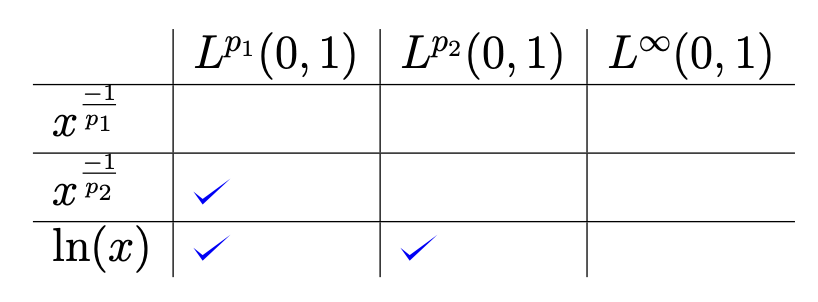
\includegraphics[height=6cm,width=12cm]{ga2}
   \end{minipage}
\end{center}
However, the relationship can be different on infinite domain, as we have the following diagram.  
\begin{center}
   \begin{minipage}{0.9\linewidth}  
       \centering
       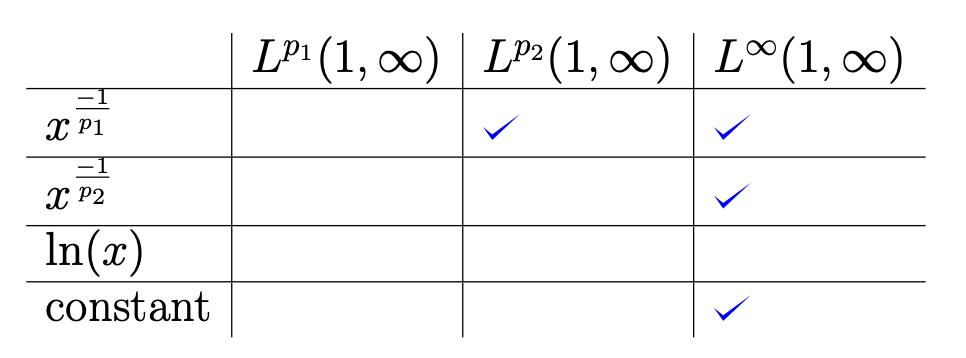
\includegraphics[height=6cm,width=12cm]{ga3}
   \end{minipage}
\end{center}
Notably, if $f$ is bounded on $E$, then we may deduce  $f \in L^{p_2}(E)$ from $f \in L^{p_1}(E)$ regardless whether $\abso{E}$ is finite.
\end{mdframed}
\begin{theorem}
\textbf{(Bounded functions in $L^p$)} If $f$ is essentially bounded on  $E$, then 
\begin{align*}
f\in L^{p_1}(E) \implies  f\in L^{p_2}(E)
\end{align*}
\end{theorem}
\begin{proof}
Note that $\abso{\set{\abso{f}>1}}\inr$ because $f\in L^{p_1}$. Let 
\begin{align*}
M\triangleq \esssup_E \abso{f} \inr
\end{align*}
The proof follows from the estimation 
 \begin{align*}
\int_E \abso{f}^{p_2}&= \int_{\set{\abso{f}\leq 1}} \abso{f}^{p_2} + \int_{\set{\abso{f}>1}} \abso{f}^{p_2}\\
&\leq \int_E \abso{f}^{p_1}+ M^{p_2} \abso{\bset{\abso{f}>1}} \inr
\end{align*}
\end{proof}
\begin{mdframed}
  Before we proceed to prove \customref{YI}{Young's inequality for product},  \customref{HI}{Holder's Inequality} and \customref{MI}{Minkowski's Inequality}, we first need  \customref{PYI}{a geometric estimation}, in which we do consider when one of  $a,b$ is infinite.  
\end{mdframed}
\begin{lemma}
\label{PYI}
\textbf{(A geometric estimation)} If $\phi:[0,\infty)\rightarrow \R$ is continuous and strictly increasing, then for all $a,b \in [0,\infty]$, 
\begin{align*}
ab\leq  \int_0^a \phi (x)dx + \int_0^b \psi(y)dy
\end{align*}
where $\psi: [0,\infty)\rightarrow \R$ is the inverse function of $\phi$. The equality hold true only when $a=b$.  
\end{lemma}
\begin{proof}
The proof follows from observing 
\begin{center}
   \begin{minipage}{0.9\linewidth}  
       \centering       
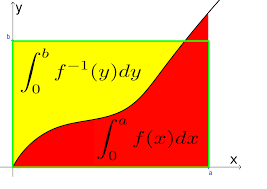
\includegraphics[height=4cm,width=8cm]{young}
   \end{minipage}
\end{center}
\end{proof}
\begin{mdframed}
Given a pair of numbers $p,q\in [1,\infty]$, we say they are \textbf{exponential conjugated} if 
\begin{align*}
\frac{1}{p}+ \frac{1}{q}= 1
\end{align*}
To make the statements of the rest of the great inequality simpler, we shall suppose from now on that $p \in [1,\infty]$ and $q$ is by default the exponential conjugate of  $p$. 
\end{mdframed}
\begin{theorem}
\label{YIfp}
\textbf{(Young's Inequality for product)} If $a,b \in [0,\infty]$ and $1< p < \infty$, then 
\begin{align*}
  ab \leq  \frac{a^p}{p} + \frac{b^q}{q}
\end{align*}
\end{theorem}
\begin{proof}
Define $\phi :[0,\infty)\rightarrow \R$ by 
\begin{align*}
\phi (x)\triangleq x^{p-1}
\end{align*}
Because $p>1$, $\phi$ is clearly continuous and strictly increasing and have the inverse $\psi : [0,\infty]\rightarrow \R$ 
\begin{align*}
\psi (y)=  y^{ \frac{1}{p-1}}
\end{align*}
It then follows from \customref{PYI}{our earlier geometric estimation} that 
\begin{align*}
  ab &\leq \int_0^a \phi (x)dx+ \int_0^b \psi (y)dy \\
  &= \frac{x^p}{p}\Big|_{x=0}^a + \frac{y ^q}{q}\Big|_{y=0}^b = \frac{a^p}{p} + \frac{b^q}{q}
\end{align*}
\end{proof}
\begin{mdframed}
Using \customref{YI}{Young's Inequality for product}, we may now prove \customref{HI}{Holder's Inequality}. 
\end{mdframed}
\begin{theorem}
\label{HI}
\textbf{(Holder's Inequality)} Let $f,g$ be two functions measurable on $E$. We have 
 \begin{align*}
\norm{fg}_1 \leq \norm{f}_p \norm{g}_q
\end{align*}
\end{theorem}
\begin{proof}
The proof is trivial if $p=1\text{ or }\infty$, so we may suppose
\begin{align*}
1< p <\infty
\end{align*}
Now, if $\norm{f}_p=0$, then $f=0$ almost everywhere, which renders the inequality trivial since $\norm{fg}_1=0$. If $\norm{f}_p=\infty$, the proof is again trivial. We may now suppose  
\begin{align*}
\norm{f}_p , \norm{g}_q \in (0,\infty)
\end{align*}
Define $f_1,g_1$ by 
\begin{align*}
f_1 \triangleq \frac{f}{\norm{f}_p} \text{ and }g_1 \triangleq \frac{g}{\norm{g}_q}
\end{align*}
Because $1<p<\infty$, by  \customref{YIfp}{Young's Inequality for product}, we have
\begin{align*}
  \norm{f_1g_1}_1=\int_E \abso{f_1g_1} &\leq \int_E \Big( \frac{\abso{f_1}^p}{p}+ \frac{\abso{g_1}^q}{q} \Big) \\
&= \frac{\norm{f_1}_p^p}{p} + \frac{\norm{g_1}_q^q}{q}= \frac{1}{p}+ \frac{1}{q}=1
\end{align*}
The proof then follows the assumption $\norm{f}_p,\norm{g}_q \in (0,\infty)$ and  
\begin{align*}
\norm{f_1g_1}_1= \frac{\norm{fg}_1}{\norm{f}_p \norm{g}_q}
\end{align*}
\end{proof}
\begin{mdframed}
What's interesting is that if we define $\langle \cdot , \cdot\rangle :L^2(E)\rightarrow \C$ by 
\begin{align*}
\langle f,g\rangle \triangleq \int f \overline{g}d\textbf{x}
\end{align*}
then $\langle \cdot, \cdot \rangle $ clearly form a positive semi-definite Hermitian form, and induce $\norm{\cdot}_2$. This with standard linear algebra immediately shows that $\norm{\cdot}_2$ satisfies the triangle inequality thus the induced $\norm{\cdot}_2$ forms a semi-norm on $L^2(E)$. Moreover, \customref{CSI}{General Cauchy-Schwarz Inequality} takes the following form on $L^2(E)$ 
\begin{align*}
 \abso{\int f \overline{g}d\textbf{x}}=\abso{\langle f,g\rangle }\leq \norm{f}_2 \cdot \norm{g}_2 
\end{align*}
which is implied by the  \customref{HI}{Holder's inequality} when $p=2$, 
\begin{align*}
\abso{\int f \overline{g}d\textbf{x}} \leq \int \abso{fg}d \textbf{x} = \norm{fg}_1 \leq \norm{f}_2 \norm{g}_2 
\end{align*}
Although it was easily shown that $L^2(E)$ is semi-normed space, to prove the same for $p \in [1,\infty]\setminus \set{2}$ is non-trivial.   
\end{mdframed}
\begin{theorem}
\label{MI}
\textbf{(Minkowski's Inequality)} For all $f,g$ measurable on  $E$  
\begin{align*}
\norm{f+g}_p \leq \norm{f}_p + \norm{g}_p
\end{align*}
\end{theorem}
\begin{proof}
If $p=1$ or  $p=\infty$, then the proof follows from noting 
\begin{align*}
\abso{f+g}\leq \abso{f}+ \abso{g}
\end{align*}
Suppose $1< p < \infty$. Let $q$ be the exponential conjugate of  $p$. Applying \customref{HI}{Holder's Inequality}, we have 
\begin{align*}
\int \abso{f+g}^{p} &= \int \abso{f+g}^{p-1} \abso{f+g} \\
&\leq \int \abso{f+g}^{p-1} \abso{f} + \int \abso{f+g}^{p-1} \abso{g} \\
&= \bnorm{\abso{f+g}^{p-1}f}_1 + \bnorm{\abso{f+g}^{p-1}g}_1 \\
&\leq \bnorm{\abso{f+g}^{p-1}}_q \cdot \norm{f}_p + \bnorm{\abso{f+g}^{p-1}}_q \cdot \norm{g}_p \\
&= \Big(\int \abso{f+g}^{p} \Big)^{\frac{1}{q}} \cdot (\norm{f}_p + \norm{g}_p)
\end{align*}
Because the proof is trivial for $\norm{f+g}_p=0\text{ or }\infty$, we may  divide both side with $(\int \abso{f+g}^{p})^{\frac{1}{q}}$ and get 
\begin{align*}
\norm{f+g}_p=\Big( \int \abso{f+g}^p \Big)^{\frac{1}{p}}= \Big( \int \abso{f+g}^p \Big)^{1- \frac{1}{q}}\leq \norm{f}_p + \norm{g}_p
\end{align*}
\end{proof}
\begin{mdframed}
What's significant about \customref{MI}{Minkowski's Inequality} is that it shows that $L^{p}(E)$ form a semi-normed space for $1\leq p\leq \infty$. To make the presentation of the proof of the next Theorem simpler, we adapt the notation 
\begin{align*}
  (\operatorname{sgn}f)(\textbf{x})\triangleq \begin{cases}
    1& \text{ if $f(\textbf{x})\geq 0$ }\\
    -1& \text{ if $f(\textbf{x})<0$ }
  \end{cases}
\end{align*}
\end{mdframed}
\begin{theorem}
\textbf{(Alternative characterization of $L^p$ norm for real-valued function)} If $f$ is real-valued and measurable on  $E$ and  $1\leq p\leq \infty$, then 
\begin{align*}
\norm{f}_p = \sup_g \int_E fg
\end{align*}
where the supremum run through all $g$ such that  $\int_E fg$ exists and $\norm{g}_q \leq 1$. 
\end{theorem}
\begin{proof}
The inequality 
\begin{align*}
\sup_g \int_E fg \leq \norm{f}_p
\end{align*}
follows from \customref{HI}{Holder's Inequality}. We now prove the opposite, by splitting into three cases 
\begin{enumerate}[label=(\alph*)]
  \item $\vi{p=1}$.  
  \item $\blue{1< p < \infty}$. 
  \item $\olive{p=\infty}$. 
\end{enumerate} 
\vi{Let $p=1$, so $q=\infty$}. Define $h \triangleq \operatorname{sgn}f$. It is clear that $\norm{h}_{\infty}=1$. Moreover, because $f\in L^1(E)$, 
\begin{align*}
\int_E fh= \int_E \abso{f}\text{ exists. }
\end{align*}
The inequality is now trivial 
\begin{align*}
\norm{f}_1 = \int_E \abso{f}= \int_E fh\leq \sup_g \int_E fg \vdone
\end{align*}
\blue{Let $1<p<\infty$}. Because the proof is trivial for $\norm{f}_p=0$, suppose $\norm{f}_p >0$. Now, divide the proof into two sub-cases 
\begin{enumerate}[label=(\alph*)]
  \item $\teal{\norm{f}_p<\infty}$. 
  \item $\orange{\norm{f}_p=\infty}$.  
\end{enumerate}
\teal{Let $\norm{f}_p<\infty$}. Define 
\begin{align}
\label{hsgn}
h\triangleq (\operatorname{sgn}f) \Big( \frac{\abso{f}}{\norm{f}_p} \Big) ^{ \frac{p}{q}}
\end{align}
Direct computation may verify $\norm{h}_q=1$ and 
\begin{align*}
  \int_E fh=\int_E \abso{fh} = \norm{f}_p \inr
\end{align*}
The proof then easily follows  
\begin{align*}
  \norm{f}_p =\int_E fh \leq \sup_g \int_E fg \tdone
\end{align*}
\orange{Let $\norm{f}_p= \infty$}. Define $f_n$ by 
\begin{align*}
f_n(\textbf{x})\triangleq \begin{cases}
  0& \text{ if $\abso{\textbf{x}}>n$ }\\
  \min \set{f(\textbf{x}),n}& \text{ if $\abso{\textbf{x}}\leq n$ } 
\end{cases}
\end{align*}
Because $f_n$ is only non-zero on $\abso{\textbf{x}}\leq n$ and is bounded by  $n$, we know $f_n \in L^p(E)$. Moreover, because $f_n\nearrow f$, by \customref{MCT}{Monotone Convergence Theorem}, 
\begin{align*}
\norm{f_n}_p \to \norm{f}_p = \infty
\end{align*}
Similar to \myref{Equation}{hsgn} in the proof of the \teal{teal sub-case}, define $h_n$ by 
\begin{align*}
h_n(\textbf{x})\triangleq \begin{cases}
  (\operatorname{sgn}f_n) \Big( \frac{\abso{f_n}}{\norm{f_n}_p} \Big) ^{ \frac{p}{q}}& \text{ if $\abso{\textbf{x}}\leq n$ }\\
  0& \text{ if $\abso{\textbf{x}}>n$ }
\end{cases} 
\end{align*}
Again, direct computation verifies $\norm{h_n}_q=1$ and  
 \begin{align*}
   \int_E f_nh_n = \int_E \abso{f_nh_n}= \norm{f_n}_p \inr
\end{align*}
The proof then follows from 
\begin{align*}
\sup_g \int_E fg\geq \int_E fh_n \geq \int_E f_nh_n = \norm{f_n}_p \ordone 
\end{align*}
\olive{Let $p=\infty$}. Again, the proof is trivial for $\norm{f}_{\infty}=0$. If $\norm{f}_{\infty}<\infty$, define 
\begin{align*}
E_n \triangleq \bset{\textbf{x}\in E: \abso{f(\textbf{x})}> \norm{f}_\infty - \frac{1}{n}}
\end{align*}
If $\norm{f}_{\infty}=\infty$, define 
\begin{align*}
E_n \triangleq \bset{\textbf{x} \in E: \abso{f(\textbf{x})}> n}
\end{align*}
In either case, $\abso{E_n}>0$ by definition. Therefore, we may find $h_n$ that share the same sign with $f$ everywhere and satisfy   
\begin{align*}
\int_{E}\abso{h_n}=1\text{ and }h_n(\textbf{x})=0\text{ for all }\textbf{x}\not\in E_n
\end{align*}
Note that  $\int fh_n$  exists because $f$ and  $h_n$ share the same sign. If $\norm{f}_{\infty}<\infty$, the proof follows from 
\begin{align*}
\sup_g \int_E fg\geq \int_E fh_n \geq \int_{E_n} (\norm{f}_{\infty}- \frac{1}{n}) \abso{h_n}= \norm{f}_{\infty} - \frac{1}{n} 
\end{align*}
If $\norm{f}_{\infty}=\infty$, the proof follows from 
\begin{align*}
\sup_g \int_E fg \geq \int_E fh_n \geq \int_{E_n} n \abso{h_n}= n \odone
\end{align*}

\end{proof}
\chapter{Harmonic Analysis}
\section{Weierstrass approximation Theorem: $[a,b]\rightarrow \R$}
\begin{theorem}
\label{Bernoulli's Inequality}
\textbf{(Bernoulli's Inequality)} Given $r,x \in\R$, suppose 
\begin{enumerate}[label=(\alph*)]
  \item $r\geq 1$ 
  \item $x\geq -1$
\end{enumerate}
Then
\begin{align*}
  (1+x)^r\geq 1+rx
\end{align*}
\end{theorem}
\begin{proof}
Fix $r\geq 1$. We wish 
\begin{align*}
\vi{\text{ to prove }(1+x)^r\geq 1+rx\text{ for all  }x \geq -1}
\end{align*}
Define $f:[-1,\infty)\rightarrow \R$ by 
 \begin{align}
\label{Bere1}
f(x)=(1+x)^r-(1+rx)
\end{align}
We reduced the problem into  
\begin{align*}
\vi{\text{ proving }f(x)\geq 0\text{ for all } x\geq -1}
\end{align*}
Because $r\geq 1$ by premise, by definition of $f(x)$  (\myref{Equation}{Bere1}), we see that 
\begin{align*}
f(0)=0\text{, and }f(-1)=r-1\geq 0
\end{align*}
Notice that by definition of $f$  (\myref{Equation}{Bere1}),  $f(x)$ is clearly differentiable on $(-1,\infty)$.\\

Then, by MVT (\myref{Theorem}{MVT}), to prove $f(x)\geq 0$ on $(-1,\infty)$, we only wish 
\begin{align*}
\vi{\text{ to prove }f'(x)\geq 0\text{ for all }x> 0\text{ and }f'(x)\leq 0\text{ for all $x \in (-1,0)$ }}
\end{align*}
Compute $f'$
 \begin{align*}
f'(x)&=r(1+x)^{r-1}-r\\
&=r\Big((1+x)^{r-1}-1 \Big)
\end{align*}
Because $r\geq 1$, we can deduce 
\begin{align*}
x>0 \implies (1+x)^{r-1}\geq 1 \implies f'(x)=r\Big((1+x)^{r-1}-1 \Big)\geq 0
\end{align*}
and deduce 
\begin{align*}
x \in (-1,0) \implies 1+x \in (0,1) \implies (1+x)^{r-1}\leq 1 \implies f'(x)=r\Big((1+x)^{r-1}-1 \Big)\leq  0
\end{align*}
$\vdone$
\end{proof}
\begin{mdframed}
In this section, notation  $\mathcal{C}\big([a,b] \big)$ means the set of \textbf{real-valued continuous function on $[a,b]$}.
\end{mdframed}
\begin{theorem}
\label{WaT}
\textbf{(Weierstrass approximation Theorem: $[a,b]\rightarrow \R$)} Let $\R[x]\big|_{[a,b]}$ be the space of polynomials on $[a,b]$ with real coefficient. We have 
\begin{align*}
\text{ $\R[x]\big|_{[a,b]}$ is dense in $\Big(\mathcal{C}\big([a,b] \big),\norm{\cdot}_{\infty} \Big)$ }
\end{align*}
\end{theorem}
\begin{proof}
WOLG, we can let $[a,b]=[0,1]$. The reason we can assume such is explained at last. Now, let $f:[0,1]\rightarrow \R$ be a continuous function. Fix $\epsilon $. We only wish 
\begin{align*}
\vi{\text{ to find $P \in \R[x]\big|_{[0,1]}$ such that $\norm{f-P}_{\infty}<\epsilon $}}
\end{align*}
Define $\tilde{f} \in \mathcal{C}\big([0,1] \big)$ by 
\begin{align}
  \label{tse1}
\tilde{f}(x)= f(x)-f(0)-x \big[f(1)-f(0) \big] 
\end{align}
It is easy to check $\tilde{f}$ is continuous. We first prove that 
\begin{align*}
\blue{\big( \tilde{f}(x)-f(x)\big)\in \R[x]\big|_{[0,1]}  }
\end{align*}
By definition of $\tilde{f} $ (\myref{Equation}{tse1}), we see 
\begin{align*}
\tilde{f}(x)-f(x)=(f(0)-f(1))x- f(0)\in \R[x]\big|_{[0,1]}\bdone
\end{align*}
This reduce our problem into 
\begin{align*}
\vi{\text{ finding }P\in \R[x]\big|_{[0,1]}\text{ such that $\norm{\tilde{f}-P}_{\infty}<\epsilon $ }}
\end{align*}
Notice that by definition of $\tilde{f}$ (\myref{Equation}{tse1}), we have 
\begin{align*}
\tilde{f}(0)=0=\tilde{f}(1) 
\end{align*}
Then, we can expand the definition of $\tilde{f} $  by
\begin{align}
\label{tse2}  
\tilde{f}(x)=\begin{cases}
  \tilde{f} (x)& \text{ if $x\in [0,1]$ }\\
  0& \text{ if $x \not \in [0,1]$ }
\end{cases}
\end{align}
This makes $\tilde{f}$ uniformly continuous on $\R$, since  $\tilde{f}$ is uniformly continuous on $[0,1]$ and $[0,1]^c$. Now, for each $n\inn$, define $Q_n \in \R[x]$ by 
\begin{align}
\label{tse3}
Q_n=c_n(1-x^2)^n\text{ where $c_n$ is chosen to satisfy }\int_{-1}^1 Q_n(x)dx=1
\end{align}
Define $P_n:[0,1]\rightarrow \R$ by 
\begin{align*}
P_n(x)=\int_{-1}^1 \tilde{f} (x+t)Q_n(t)dt
\end{align*}
We now prove 
\begin{align*}
\olive{P_n \in \R[x]\big|_{[0,1]}}
\end{align*}
Because $\tilde{f}(x)=0$ for all $x \not \in (0,1)$ by definition of $\tilde{f} $ (\myref{Equation}{tse2}), we see that 
\begin{align}
\label{tse4}
P_n(x)=\int_{-x}^{1-x}\tilde{f}(x+t)Q_n(t)dt \text{ for all }x \in [0,1]
\end{align}
Fix $x \in [0,1]$. Now, by change of variable, we see 
\begin{align*}
P_n(x)=\int_{-x}^{1-x} \tilde{f}(x+t)Q_n(t)dt=\int_{0}^1 \tilde{f}(u)Q_n(u-x)du  
\end{align*}
Because $Q_n$ is a polynomial by definition (\myref{Equation}{tse3}), we can express $Q_n(u-x)$ by 
\begin{align*}
Q_n(u-x)=\sum_{k=0}^{m} a_k x^k\text{ for some $\set{a_0,\dots ,a_m}$ depending on $u$}
\end{align*}
Then we see 
\begin{align*}
  P_n(x)=\int_0^1 \tilde{f}(u)Q_n(u-x)du= \sum_{k=0}^m x^k \Big( 
\int_0^1 \tilde{f}(u) a_kdu
  \Big)  
\end{align*}
This shows that $P_n \inr[x]\big|_{[0,1]}$

$\odone$\\


Now, because $\tilde{f}$ is uniformly continuous on $\R$, we can fix $\delta<1$ such that 
\begin{align}
\label{tse5}
\forall x,y \inr, \abso{x-y}<\delta \implies \abso{\tilde{f}(x)-\tilde{f}(y)  }<\frac{\epsilon}{2}
\end{align}
By definition of $\tilde{f}$ (\myref{Equation}{tse2}), we know $\tilde{f} $ is a bounded function. Then we can set $M$ by 
\begin{align*}
M=\sup_{x \inr} \abso{f(x)}
\end{align*}
Let $n$ satisfy 
 \begin{align}
  \label{tse5}
4M \sqrt{n} (1-\delta^2)^n < \frac{\epsilon}{2} 
\end{align}
Such $n$ exists, because  $\delta<1 \implies  \sqrt{n}(1-\delta^2)^n \to 0 $. We claim 
\begin{align*}
\vi{\text{ $P_n$ satisfy $\norm{\tilde{f}-P_n}_{\infty}<\epsilon $}}
\end{align*}
We first prove 
\begin{align*}
\blue{c_n< \sqrt{n} }
\end{align*}
By Bernoulli's Inequality (\myref{Theorem}{Bernoulli's Inequality}). Compute 
\begin{align*}
1=\int_{-1}^1 Q_n(x)dx&=  c_n\int_{-1}^1 (1-x^2)^n dx \\
&=2c_n\int_0^1 (1-x^2)^n dx\\
&\geq 2c_n\int_0^{\frac{1}{\sqrt{n} }}(1-x^2)^n dx\\
&\geq 2c_n \int_0^{\frac{1}{\sqrt{n} }} 1-nx^2dx=c_n\big(\frac{4}{3\sqrt{n} } \big)> c_n (\frac{1}{\sqrt{n} })
\end{align*}


This implies 
\begin{align*}
\sqrt{n}>c_n \bdone
\end{align*}
Because $\sqrt{n}>c_n $, by definition of $Q_n$  (\myref{Equation}{tse3}), we have 
\begin{align*}
Q_n(x)<\sqrt{n}(1-x^2)^n \leq \sqrt{n}(1-\delta^2)^n \text{ for all $x$ such that  $\delta \leq \abso{x}\leq 1$ }
\end{align*}
Fix $x \in [0,1]$. Finally, because 
\begin{enumerate}[label=(\alph*)]
  \item $\int_{-1}^1 Q_n(x)dx=1$ by definition of  $Q_n$  (\myref{Equation}{tse3})
  \item $Q_n(x)=c_n(1-x^2)^n\geq 0$ for all $x \in [-1,1]$ 
  \item $\abso{\tilde{f}(x+t)-\tilde{f}(x)}<\frac{\epsilon}{2} $ for all $t$ such that $\abso{t}<\delta $, by definition of $\delta $ (\myref{Equation}{tse5})
  \item $Q_n(x)\leq \sqrt{n}(1-\delta^2)^n $ for all $x$ such that  $\delta\leq \abso{x}\leq 1$
  \item $4M\sqrt{n}(1-\delta^2)^n<\frac{\epsilon}{2} $ by definition of $n$  (\myref{Equation}{tse5})
\end{enumerate}
we have
\begin{align*}
\abso{P_n(x)-\tilde{f}(x)}&=\abso{\int_{-1}^1 \tilde{f}(x+t)Q_n(t)dt- \tilde{f}(x)}\\
&=\abso{\int_{-1}^1 \tilde{f}(x+t)Q_n(t)dt- \tilde{f}(x)\int_{-1}^1 Q_n(t)dt }\\
&=\abso{\int_{-1}^1 \tilde{f}(x+t)Q_n(t)dt -\int_{-1}^1 \tilde{f}(x)Q_n(t)dt}\\
&=\abso{\int_{-1}^1 \big[\tilde{f}(x+t)-\tilde{f}(x)   \big]Q_n(t)dt}\\
&\leq \int_{-1}^1 \abso{\big[ \tilde{f}(x+t)-\tilde{f}(x)\big]Q_n(t)}dt\\
&=\int_{-1}^1 \abso{\tilde{f}(x+t)-\tilde{f}(x)  }Q_n(t)dt\\
&\leq \int_{-1}^{-\delta} 2MQ_n(t)dt +\int_{-\delta}^{\delta} \abso{\tilde{f}(x+t)-\tilde{f}(x)  }Q_n(t)dt+\int_{\delta}^1 2M Q_n(t)dt\\
&\leq 2M\Big(\int_{-1}^{-\delta}Q_n(t)dt+\int_{\delta}^1 Q_n(t)dt  \Big)+ \int_{-\delta}^\delta \big(\frac{\epsilon}{2} \big)Q_n(t)dt\\
&\leq 4M(1-\delta) \sqrt{n}(1-\delta^2)^n+ \frac{\epsilon}{2} \\
&\leq 4M\sqrt{n}(1-\delta^2)^n+\frac{\epsilon}{2} <\epsilon  
\end{align*}
Because $x$ is arbitrarily picked from  $[0,1]$, we now have $\norm{P_n-\tilde{f} }_{\infty}<\epsilon \vdone$\\

Lastly, we show 
\begin{align*}
\olive{\text{ our result can be transplanted to arbitrary $\mathcal{C}\big([a,b] \big)$ }}
\end{align*}
Let $[a,b]$ be arbitrary. Fix $\epsilon $ and $f \in \mathcal{C}\big([a,b] \big)$. We wish 
\begin{align*}
\olive{\text{ to find $P \in \R[x]\big|_{[a,b]}$ such that $\norm{f-P}_\infty\leq \epsilon $ }}
\end{align*}
Define $g:[0,1]\rightarrow \R$ by 
\begin{align}
g(x)\triangleq f(a+(b-a)x)
\end{align}
We know there exists $P_n:[0,1]\rightarrow \R$ such that 
\begin{align*}
\norm{P_n-g}_{\infty}<\epsilon 
\end{align*}
Define $H_n:[a,b]\rightarrow \R$ by 
\begin{align*}
H_n(x)=P_n\big(\frac{x-a}{b-a} \big)
\end{align*}
Because $P_n$ is a real polynomial on  $[0,1]$, we know $H_n$ is a real polynomial on $[a,b]$. We now claim 
\begin{align*}
  \olive{\text{ such $H_n\text{ works }$ }}
\end{align*}
Fix $x \in [a,b]$. Observe 
\begin{align*}
\big|f(x)-H_n(x)\big|&=\abso{f(x)-P_n\big(\frac{x-a}{b-a} \big)}\\
&=\abso{g\big(\frac{x-a}{b-a} \big)-P_n\big(\frac{x-a}{b-a} \big)}< \epsilon \odone
\end{align*}
\end{proof}
\begin{mdframed}
It is at now, we will show that every real-valued continuous functions on $[a,b]$ can be approximated by polynomials with rational coefficient. This fact enable our computer to more easily approximate real-valued continuous function on $[a,b]$.\\

Note that since $\mathcal{C}\big([a,b] \big)$ is a separable metric space, we can show that $\mathcal{C}\big([a,b] \big)$ has cardinality of at most continuum $\mathfrak{c}$ . 
\end{mdframed}
\begin{theorem}
\textbf{(The space $\Q[x]|_{[a,b]}$ is dense in $\Big( \mathcal{C}\big([a,b] \big),\norm{\cdot}_{\infty}\Big)$, thus $\mathcal{C}\big([a,b] \big)$ is separable)} 
\begin{align*}
\Big( \mathcal{C}\big([a,b] \big),\norm{\cdot}_{\infty}\Big)\text{ is separable }
\end{align*}
\end{theorem}
\begin{proof}
Because $\Q[x]\big|_{[a,b]}$ is countable, to show $\mathcal{C}\big([a,b] \big)$ is separable, we only wish to show 
\begin{align*}
\vi{\Q [x]\big|_{[a,b]}\text{ is dense in }\mathcal{C}\big([a,b] \big)}
\end{align*}
Because $\R[x]\big|_{[a,b]}$ is dense in $\mathcal{C}\big([a,b] \big)$, we reduce our problem into proving 
\begin{align*}
\vi{\Q[x]\big|_{[a,b]}\text{ is dense in }\R[x]\big|_{[a,b]}}
\end{align*}
Fix $\epsilon \text{ and } P \in \R[x]\big|_{[a,b]}$. We must
\begin{align*}
\vi{\text{ find $Q \in \Q[x]\big|_{[a,b]}$ such that $\norm{Q-P}_\infty \leq \epsilon $}}
\end{align*}
Express $P(x)=\sum_{k=0}^n r_kx^k$. Let $M> \max \set{\abso{a},\abso{b}}$. Because $\Q$ is dense in $\R$, we know there exists $c_k \inq$ such that  $\abso{c_k-r_k}< \frac{\epsilon }{(n+1)M^n}$. We claim 
\begin{align*}
\vi{Q(x)=\sum_{k=0}^n c_kx^k\text{ works }}
\end{align*}
Fix $x \in [a,b]$. See
\begin{align*}
\abso{P(x)-Q(x)}&=\abso{\sum_{k=0}^n (c_k-r_k)x^k}\\
&\leq \sum_{k=0}^n \abso{c_k-r_k}\cdot \abso{x}^k\\
&\leq \sum_{k=0}^n \abso{c_k-r_k}\cdot M^k\\
&\leq (M^n)\sum_{k=0}^n \abso{c_k-r_k}\\
&< M^n (n+1)\big( \frac{\epsilon }{(n+1)M^n}\big)=\epsilon \vdone
\end{align*}
\end{proof}
\section{The Stone-Weierstrass Theorem}
\begin{mdframed}
Recall that a \textbf{vector space over a field $\F$} is a set $V$ equipped with \textbf{vector addition} $+:V\times V\to V$  and \textbf{scalar multiplication}  such that 
\begin{enumerate}[label=(\alph*)]
  \item $(V,+)$ is an abelian group. 
  \item Scalar multiplication is compatible with field multiplication:   $\Big((ab)v=a(bv) \Big)$
  \item Scalar multiplication is distributive: $\Big((a+b)v=av+bv\text{ and }a(v+w)=av+aw \Big)$
\end{enumerate}

There are many ways to define the term \textbf{algebra over a field $\F$}. One can exhaust all the laws an algebra should obey. In short, an \textbf{algebra over a field $\F$} (or \textbf{$\F$-algebra}) is a vector space $V$ equipped with a vector multiplication such that  
\begin{enumerate}[label=(\roman*)]
  \item Multiplication is $\underline{\text{distributive}}$ to addition. 
   \item Scalar and vector multiplications are compatible: $(av)\cdot (bw)=ab(v\cdot w)$
\end{enumerate}
Given an arbitrary set $E$ and a field $\F$, let $A$ be the set of all functions from  $E$ to $\F$. The following is a list of some algebra 
\begin{enumerate}[label=(\alph*)]
  \item $(\R^3,\text{cross product})$  over $\R$ 
  \item $(\C,\text{complex multiplication})$ over $\C$ 
  \item $(\Q[x],\text{function multiplication})$ over $\Q$
  \item $(\text{Functions from }E\text{ to }\F,\text{function multiplication})$ over $\F$
  \item $(\text{Continuous functions from $(E,\tau)$ to $\C$ },\text{function multiplication})$ over $\C$  
  \item $(\text{Linear transformation from $V$ to $V$, composition})$ over $\F$ where  $V$ is over $\F$
  \item $\big(M_n(\F),\text{matrix multiplication}\big)$ over $\F$
\end{enumerate}
Note that $B=(\text{continuous functions from }\C\text{ to }\C,\text{composition})$ over $\C$ is not an algebra, even though $B$ is both a vector space and a ring. ($\because$ scalar multiplication and multiplication are not compatible).\\

It is at here we shall introduce some general terminologies. Given an arbitrary set $E$, a field  $\F$ and a point $x \in E$, we say a family $\mathcal{F}$ of functions  from $E$ to  $\F$  \textbf{vanish at $x$} if for all $f \in \mathcal{F}$, we have $f(x)=0$. We say $\mathcal{F}$ \textbf{separate points} in $E$ if for all  $x_2\neq x_1 \in E$, there exists $f\in \mathcal{F}$ such that $f(x_2)\neq f(x_1)$. 
\end{mdframed}
\chapter{Differential Geometry}
\label{Differentail Geometry}
\section{Smooth Manifold}
\begin{abstract}
This main goal of this section is to 
\begin{enumerate}[label=(\alph*)]
  \item introduce the idea of smooth manifolds. 
  \item prove that \customref{Smooth manifolds always admit smooth partition of unity}{smooth manifolds always admit smooth partition of unity}. 
\end{enumerate}
\end{abstract}
\begin{mdframed}
Given a topological space $(X,\mathscr{T })$ and fix $n$, if $:U\rightarrow \R^n$ is a homeomorphism between some open subspace $U$ of $X$ and some open subspace of $\R^n$, we say $(\Phi,U)$ is a \textbf{chart} on $X$, and if there exists a collection $A=\set{(\Phi_i, U_i)}_{i \in I}$ of chart cover the whole $X$, we say $A$ is an  \textbf{atlas} and  $X$ is  \textbf{locally Euclidean}.  We now give definition to the term \textbf{topological manifold}, which we will use throughout this chapter.  
\end{mdframed}
\begin{definition}
\textbf{(Definition of Topological Manifold)} We say a Topological space $X$ is a \textbf{topological manifold} if 
\begin{enumerate}[label=(\alph*)]
  \item $X$ is locally Euclidean. 
  \item $X$ is Hausdorff. 
  \item $X$ is second countable.
\end{enumerate}
\end{definition}
\begin{mdframed}
Immediately, one should check that all three conditions are necessary: There are locally Euclidean space that is not Hausdorff, \customref{Bug-Eyed Line}{Bug-Eyed Line} for example. There also are locally Euclidean space that is not second countable, \customref{Long Line}{Long Line} for example. Also, one can check that any open subspace or finite products of topological manifold is still topological manifold. To have a better understanding why we require more than locally Euclidean in our definition of topological manifol, we first introduce some more topological notions. Given a collection of subsets $(E_\alpha )$ of some topological space $X$, we say $(E_\alpha )$ is \textbf{locally finite} if for each $p \in X$, there exists some neighborhood of $p$ intersecting with only finitely many of $E_\alpha $. Given an open cover $(E_\alpha )$ of topological space $M$, we say a family of continuous function  $\psi_\alpha :M\rightarrow \R$ is a \textbf{partition of unity subordinate to (or dominated by) $(E_\alpha )$} if 
\begin{enumerate}[label=(\roman*)]
  \item $0\leq \psi_\alpha  (x)\leq 1$ for all $\alpha \in A,x\in M$. 
  \item $\operatorname{supp}\psi_\alpha  \subseteq X_\alpha $ for all $\alpha $. 
  \item The collection $\set{\operatorname{supp}\psi_\alpha \subseteq M:\alpha \in A}$ is locally finite.
  \item  $\sum_{\alpha \in A}\psi_\alpha (x)=1$ for all $x\in M$. (Note that the sum is finite because $\set{\operatorname{supp}\psi_\alpha}$ is locally finite)
\end{enumerate}


Given a cover $(E_\alpha )$ of topological space $X$, we say another cover $(F_\beta  )$ of $X$ is a  \textbf{refinement of $E$} if for each $\beta $ there exists some $\alpha $ such that $F_\beta  \subseteq E_\alpha $. Suppose we have some open cover $(U_\alpha )_{\alpha  \in A}$ of some topological space $X$    
 A topological space $X$ if said to be \textbf{paracompact} if every open cover has a locally finite open refinement. It shall be clear that each compact space is paracompact.
\end{mdframed}
\begin{theorem}
\label{Topological Manifold are Paracompact}
\textbf{(Topological Manifold are Paracompact)} Every locally compact, Hausdorff second-countable space $M$ is paracompact. Moreover, for each open cover $\mathcal{S}$ and basis $\mathcal{B}$, there exists a countable locally finite open refinement of $\mathcal{S}$ consisting of elements of $\mathcal{B}$.  
\end{theorem}
\begin{proof}
We first show that 
\begin{center}
   \begin{minipage}{0.9\linewidth}  
     \olive{$M$ admits an exhaustion by compact sets, i.e., there exists a sequence $K_n$ of compact sets  such that $M=\bigcup K_n$ and $K_n \subseteq K_{n+1}^\circ $}. 
   \end{minipage}
\end{center}
Since $M$ is locally compact and Hausdorff, we know \customref{Locally Compact Hausdorff Space admits a pre-compact basis}{there exists some basis of $X$ consisting of  precompact open sets}, and since $M$ is second countable, \customref{Basis Property of Second Countable Space}{we can WOLG write this basis as $(U_n)$}. Let $K_1\triangleq \overline{U_1}$. Now, since $(U_k)$ cover the whole $M$,  for each $n$ we can let  $m_n$ be some integer greater than  $n$ and  $K_n\subseteq U_1\cup  \cdots \cup  U_{m_n}$. Defining $K_{n+1}\triangleq \overline{U_1}\cup  \cdots \cup \overline{U_{m_n}}$, we see $K_{n+1}$ is compact because it is a finite union of compact subspace. We also see $K_n \subseteq U_1 \cup \cdots \cup  U_{m_n}\subseteq K_{n+1}^{\circ }$. $\odone$ \\

Now, for each $n\inz_0^+$, define 
\begin{align*}
  V_n \triangleq K_{n+1}\setminus K_n^{\circ }\text{ and }W_n \triangleq K_{n+2}^{\circ } \setminus K_{n-1}\text{ where }K_0=K_{-1}=\varnothing
\end{align*}
Note that $W_n$ are open and $V_n \subseteq W_n$. We then can associate each  $n$ and $x \in V_n$ with some $S^n_x \in \mathcal{S}$ and $B^n_x \in \mathcal{B}$ such that $x \in B^n_x \subseteq S^n_x\cap W_n$. Now, because $V_n$ is compact  (closed in $K_{n+1}$), we know there exists a finite subcollection $\set{B^n_{x_1},\dots ,B^n_{x_{n_k}}}$ covering $V_n$ and contained by  $W_n$. Define 
\begin{align*}
\mathcal{S}'\triangleq \bigcup_{n\inz_0^+} \set{B^n_{x_1},\dots , B^n_{x_{n_k}}}
\end{align*}
We then see that $\mathcal{S}'$ is a countable refinement of $\mathcal{S}$ (The fact $\mathcal{S}'$ is a cover follows from $V_n$ covering the whole  $M$). To see that $\mathcal{S}'$ is locally finite, observe that each $B^n_{x_j}$ is contained by $W_n$ and if  $\abso{p-q}>2$, then $W_p\cap W_q=\varnothing$. 
\end{proof}
\begin{mdframed}
An atlas $A$ is said to be a \textbf{smooth atlas}, if for each two charts $(\Phi_i,U_i),(\Phi_j,U_j)$ in $A$, 
\begin{align*}
\text{ The function }\Phi_i\circ \Phi_j^{-1}:\Phi_j(U_i\cap U_j)\to \Phi_i(U_i\cap U_j)\text{ is a smooth diffeomorphism }
\end{align*}
It is easily checked that for each two chart $\Phi_i,\Phi_j$, the \textbf{transition map} $\Phi_i\circ \Phi_j^{-1}$ is a homeomorphism. Now, if the union of two smooth atlas $A_1,A_2$ is again smooth, we say $A_1,A_2$ are \textbf{compatible}. With some effort, one can check that compatibility is an equivalence relation on the collection of all possible atlas on $X$. Thus, it make sense for us to define the \textbf{smooth structure}, i.e., a maximal smooth atlas on $X$. Now, by a \textbf{smooth manifold}, we merely mean a manifold equipped with a maximal smooth atlas, and given a function $F:M\rightarrow N$ that maps a smooth manifold $M$ into another smooth manifold  $N$, we say  $F$ is \textbf{smooth at $p$} if $F$ is continuous at $p$ and there exists some charts $(U,\phi),(V,\psi)$ respectively at $p,F(p)$ such that 
\begin{enumerate}[label=(\roman*)]
  \item $U \subseteq F^{-1}(V)$. 
  \item $\psi \circ F\circ \phi^{-1} : \phi (U) \subseteq \R^m \rightarrow \psi (V)\subseteq \R^n\text{  is smooth at }\phi (p)$. 
\end{enumerate}
Note that $F$ is required to be continuous at $p$ in the first place to guarantee that for all $(V,\psi)$ at $F(p)$ there exists some $(U,\phi)$ at $p$ such that $F(U)\subseteq V$. Immediately, one can check that if $F$ is smooth at  $p$, then 
\begin{enumerate}[label=(\alph*)]
  \item For all charts $(U,\phi),(V,\psi)$ at $p,F(p)$, the function $\psi \circ F\circ \phi ^{-1}:\phi(F^{-1}(V)\cap U )\subseteq \R^m\rightarrow \psi  (V )\subseteq \R^n$ is smooth at $p$. 
  \item If $G:N\rightarrow R$ is another map smooth at $F(p)$, then $G\circ F:M\rightarrow R$ is smooth at $p$.  
\end{enumerate}
When $F$ is a $\R^n$-valued function on $M$, we define the smoothness of  $F$ by considering  $\R^n$ as a manifold with the standard atlas  $\set{(\R^n,\textbf{id})}$. With these definitions specified, we are almost ready to prove that smooth manifolds always admits smooth partition of unity, but before we actually give a proof, we first need to know how to manipulate smooth function between Euclidean Spaces. The simplest smooth function $\Psi:\R\rightarrow \R$ is perhaps 
\begin{align*}
\Psi (x)\triangleq \begin{cases}
  e^{\frac{-1}{1-x^2}}& \text{ if $\abso{x}<1$ }\\
  0& \text{ if $\abso{x}\geq 1$ }
\end{cases}
\end{align*}
Although the $\Psi$ we just defined is smooth, it is not particularly useful in construction of partition of unity.
\begin{center}
   \begin{minipage}{0.9\linewidth}  
       \centering
       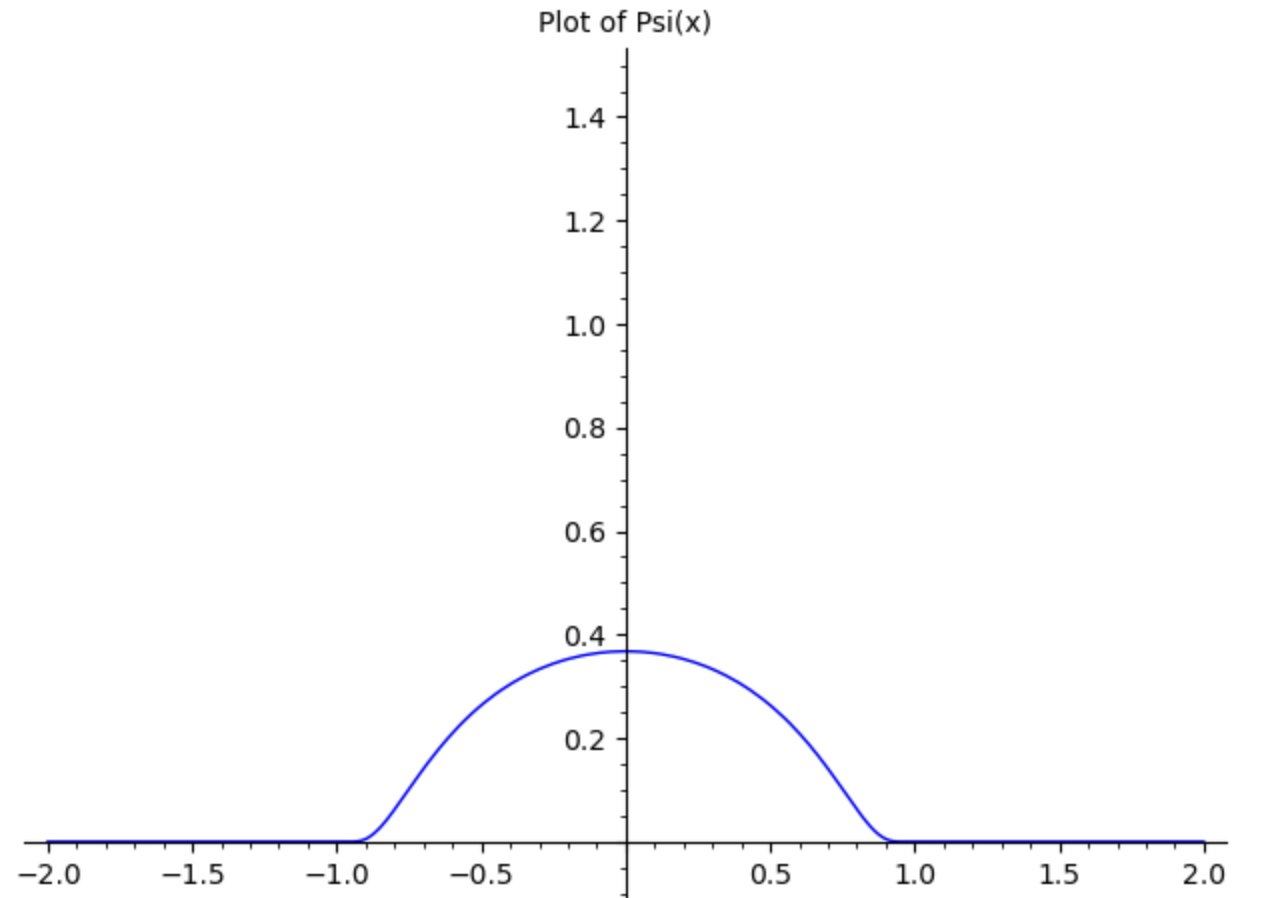
\includegraphics[height=6cm,width=16cm]{Psi_graph}
   \end{minipage}
\end{center}
Consider the smooth function $f:\R\rightarrow \R$ defined by 
\begin{align*}
f(x)\triangleq \begin{cases}
  e^{\frac{-1}{x}}& \text{ if $x>0$ }\\
  0& \text{ if $x\leq 0$ }
\end{cases}
\end{align*}
\begin{center}
   \begin{minipage}{0.9\linewidth}  
       \centering
       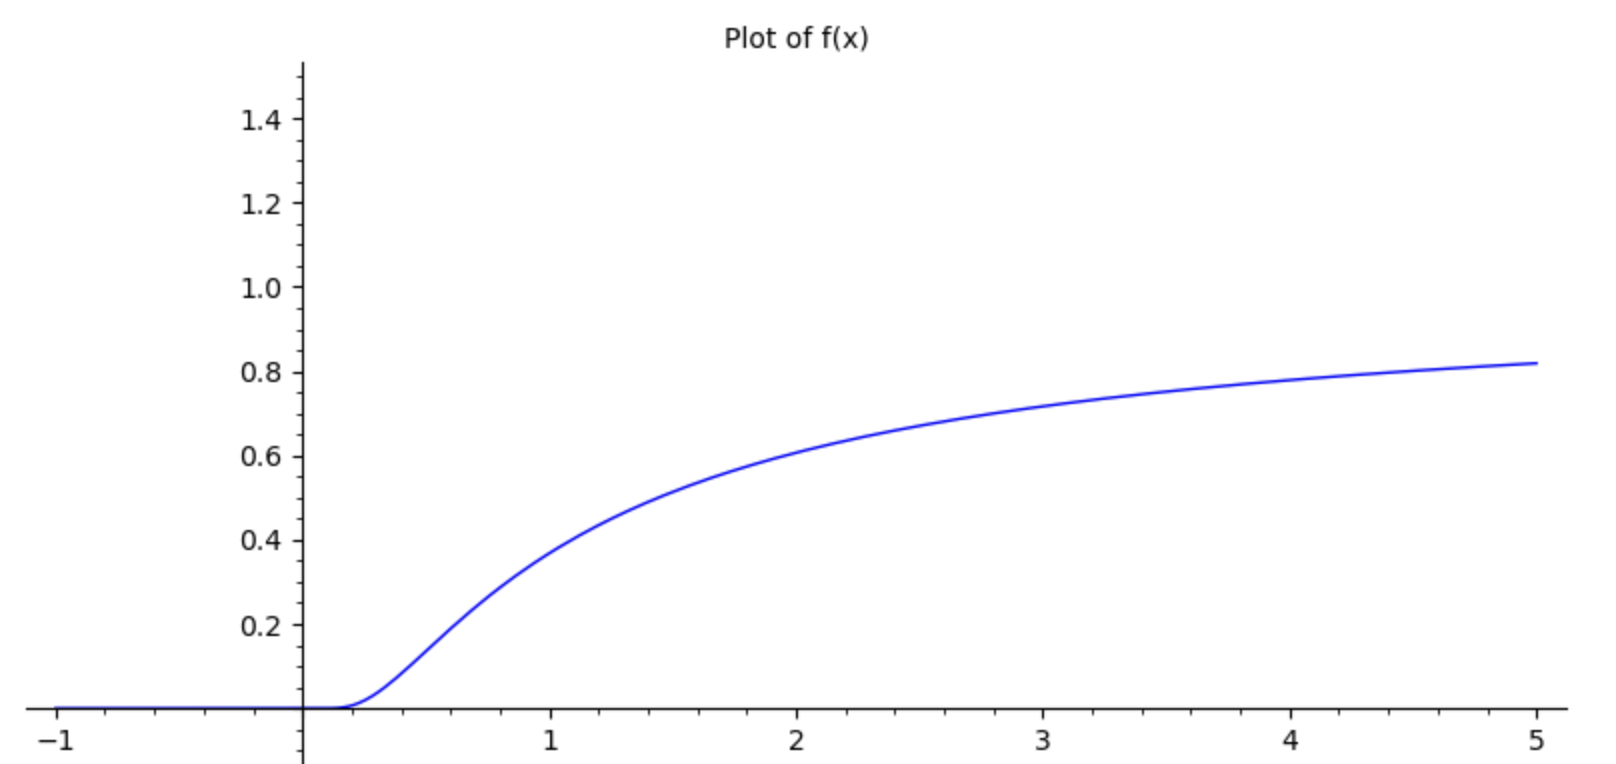
\includegraphics[height=6cm,width=16cm]{f_graph}
   \end{minipage}
\end{center}
and  $g:\R\rightarrow \R$ defined by 
\begin{align}
\label{gsm}
g(x)\triangleq \frac{f(x)}{f(x)+f(1-x)}
\end{align}
\begin{center}
   \begin{minipage}{0.9\linewidth}  
       \centering
       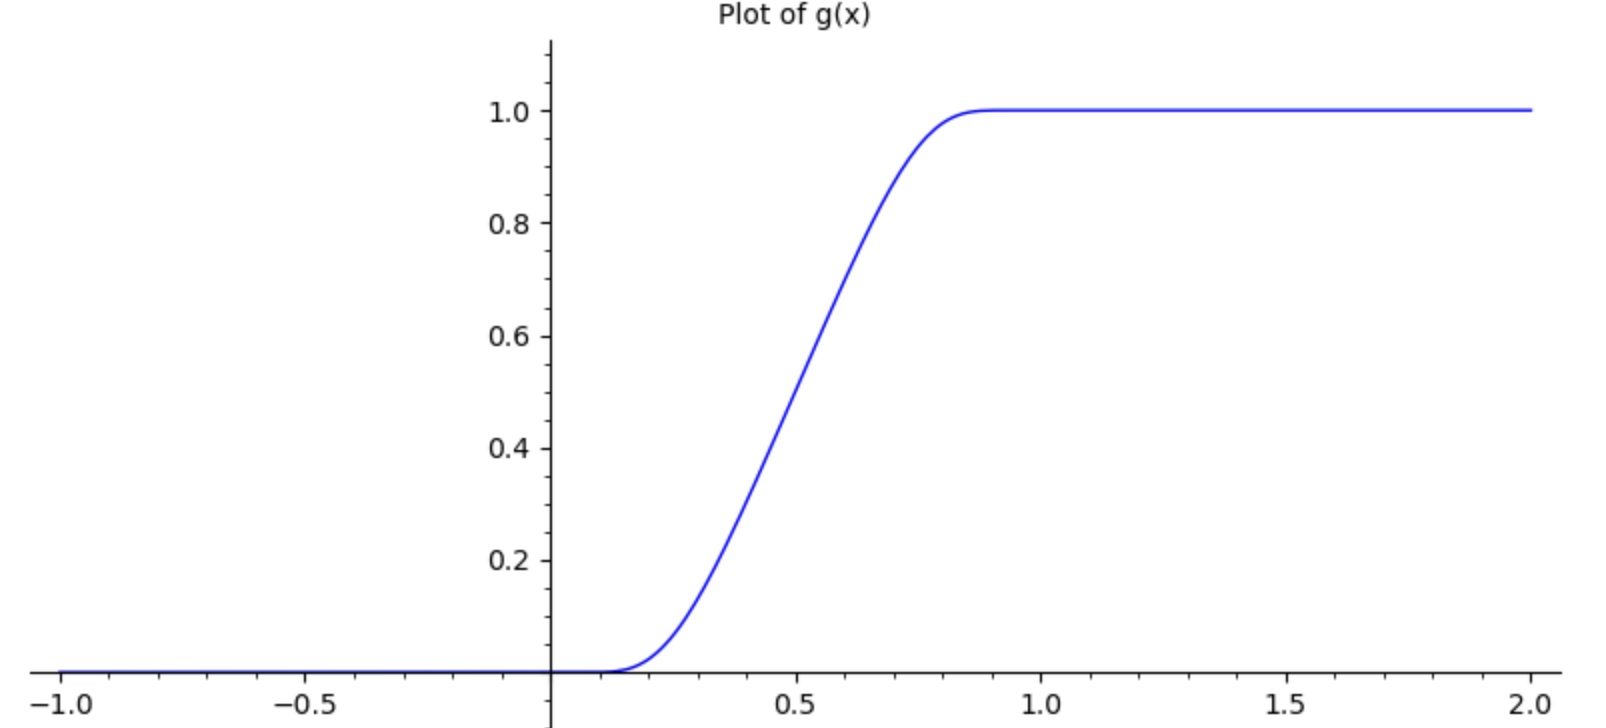
\includegraphics[height=6cm,width=16cm]{g_graph}
   \end{minipage}
\end{center}
which is a smooth increasing function such that  
\begin{align*}
g(x)=\begin{cases}
  0& \text{ if $x\leq 0$ }\\
  1& \text{ if $x\geq 1$ }
\end{cases}\text{ and }g(x)\in (0,1)\text{ if }x\in (0,1)
\end{align*}
Lastly, if we define $h:\R\rightarrow \R$ by
\begin{align*}
h(x)\triangleq g(2+x)g(2-x)
\end{align*}
\begin{center}
   \begin{minipage}{0.9\linewidth}  
       \centering
       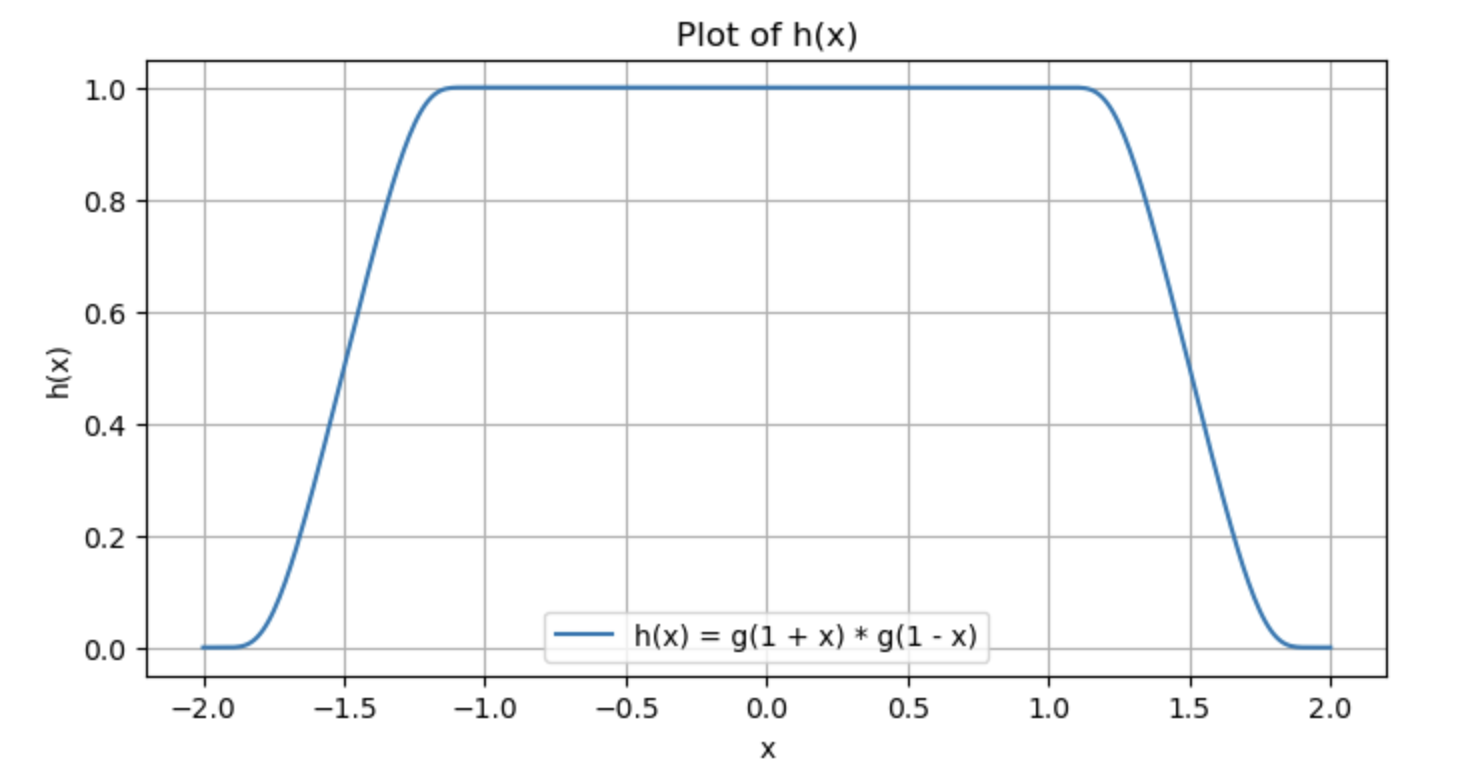
\includegraphics[height=6cm,width=16cm]{h_graph_rev}
   \end{minipage}
\end{center}
We see that $h$ is a smooth function and 
\begin{align*}
h(x)=\begin{cases}
  1& \text{ if $\abso{x}\leq 1$ }\\
  0& \text{ if $\abso{x}\geq 2$ }
\end{cases}\text{ and }h(x)\in (0,1)\text{ if } 1< \abso{x}< 2
\end{align*}
A $n$-dimensional generalization of this smooth function $h$ is  $H:\R^n\rightarrow \R$ defined by 
\begin{align*}
H(\textbf{x})\triangleq  h\Big(\frac{\abso{\textbf{x}}}{r}\Big)
\end{align*}
which is a non-negative smooth function such that 
\begin{align*}
H(\textbf{x})>0\text{ if and only if }\abso{\textbf{x}}< 2r
\end{align*}
\end{mdframed}
\begin{theorem}
\label{Smooth manifolds always admit smooth partition of unity}
\textbf{(Smooth manifolds always admit smooth partition of unity)} Given a smooth manifold $M$ and some open cover  $(U_\alpha )$ of $M$, there exists some smooth partition of unity  $(\psi_\alpha )$ subordinate to $(U_\alpha )$. 
\end{theorem}
\begin{proof}
For each $U_\alpha $ and each chart $(V,\phi)$ contained by $U_\alpha $, if we let $\mathcal{B}_{\alpha ,V}$ be the collection of the pre-images of the open balls $B_r(x)$ in $\phi (V)$ that satisfy $\exists r'>r:B_{r'}(x)\subseteq \phi (V)$, we know that $\mathcal{B}_{\alpha ,V}$ form a basis of $V$. It follows that there exists a basis $\mathcal{B}_\alpha $ for $U_\alpha $ of the form $\mathcal{B}_\alpha \triangleq \bigcup_{(V,\phi)\subseteq U_\alpha }\mathcal{B}_{\alpha ,V}$ and a basis $\mathcal{B}$ for $M$ of the form  $\mathcal{B}\triangleq \bigcup_{\alpha}\mathcal{B}_\alpha $. By \myref{Theorem}{Topological Manifold are Paracompact}, we know there exists a countable locally finite open refinement $(B_n)$ of $U_\alpha $ consisting of element of $\mathcal{B}$.\\

Now, for each $n$, there exists corresponding chart $(V,\phi)$ and $r,r'$ such that  
 \begin{align*}
   \phi (B_n)=B_r(x)\text{ and }\overline{B_r(x)}\subseteq B_{r'}(x)\subseteq \phi (V)
\end{align*}
This with some tedious effort guarantee that  
\begin{align*}
\overline{B_n}=\phi^{-1}(\overline{B_r(x)})
\end{align*}
We then can well-define a function $f_n:M\rightarrow \R$ by 
\begin{align*}
f_n \triangleq \begin{cases}
  H_n \circ \phi &\text{ on }V\\
  0&\text{ on }M\setminus \overline{B_n}
\end{cases}
\end{align*}
where $H_n:\R^n\rightarrow \R$ is a smooth function that is positive on $B_r(x)$ and zero else where. (One should at this point check that $f_n$ is well-defined)\\

Since $V$ and  $M \setminus \overline{B_n}$ are both open and $f_n$ are both smooth on them, we now see  $f_n$ is smooth on the whole  $M$. Now, since $(B_n)$ is a locally finite cover of $M$ and $f_n$ can only be positive on  $B_n$, we see that the function $f:M\rightarrow \R$ 
\begin{align*}
f(x)\triangleq \sum_{n\inn}f_n(x)\text{ is well defined }
\end{align*}
and that $f$ is positive on whole $M$  because each $f_n$ is positive on $B_n$ and $(B_n)$ cover the whole $M$. Note that $f$ is also smooth on $M$ since for each $x$, there exists an open-neighborhood around $x$ on which $f$ is just a finite sum of $f_n$. We now can define for each $n$ a smooth function  $g_n:M\rightarrow \R$ by 
\begin{align*}
g_n(x)\triangleq \frac{f_n(x)}{f(x)}
\end{align*}
Lastly, because $(B_n)$ is an open refinement of $U_\alpha $, we can associate each $n$ with an $\alpha (n)$ satisfying $B_n \subseteq U_{\alpha (n)}$. Then, because $g_n$ are non-negative and  $\sum_{n\inn}g_n\equiv 1$, we can define for each $\alpha $ a function $\psi_\alpha :M\rightarrow \R$ by 
\begin{align*}
\psi_\alpha \triangleq \sum_{n:\alpha (n)=\alpha } g_n
\end{align*}
Because $(B_n)$ is locally finite and $g_n$ is only positive on $B_n$, we see that  $\psi_\alpha $ is indeed smooth. Some tedious effort shows that $\psi_\alpha $ is indeed a partition of unity.  

\end{proof}
\begin{corollary}
\label{EoSB}
\textbf{(Existence of smooth function)} Given some  $U$ open in $M$ and some $K$ closed in $M$ and contained by  $U$, there exists a smooth function  $\psi : M\rightarrow [0,1]$ such that 
\begin{enumerate}[label=(\alph*)]
  \item $\psi \equiv 1$ on $K$. 
  \item $\operatorname{supp}\psi \subseteq U$
\end{enumerate}
\end{corollary}
\begin{corollary}
\label{EoSF}
\textbf{(Extension of Smooth Function)} Suppose $K$ is closed in $M$, and $U$ is open in  $M$ while containing  $K$. For all $f\in C^{\infty}(U)$, there exists $\tilde{f}\in C^{\infty}(M)$ such that $\tilde{f}|_K=f$ and $\operatorname{supp}\tilde{f}\subseteq U$. 
\end{corollary}
\begin{proof}
\myref{Corollary}{EoSB} give us a smooth function $\psi \in C^{\infty}(M)$ such that $\psi \equiv 1$ on $K$ and  $\operatorname{supp}\psi \subseteq U$. We simply define 
\begin{align*}
\tilde{f}(p)\triangleq \begin{cases}
  \psi(p) f (p)& \text{ if $p\in  U$ }\\
  0& \text{ if $p\not\in U$ }
\end{cases} 
\end{align*}
It is clear that $\tilde{f}|_K=f$. To see $\operatorname{supp}\tilde{f} \subseteq U$, check $\operatorname{supp}\tilde{f} \subseteq \operatorname{supp}\psi$. It is clear that $\tilde{f}$ is smooth on $U$. To see $\tilde{f}$ is smooth at all $p\not\in U$, observe that $\tilde{f}\equiv 0$ on some neighborhood around $p$. 
\end{proof}
\begin{mdframed}
Before we state the next Theorem, we shall point out that since topological manifolds are locally Euclidean, they are locally connected, and thus \customref{local-path}{the connected components of a topological manifold are identical to the path-connected components}.  
\end{mdframed}
\begin{theorem}
\textbf{(Existence of Smooth Curve)} If $p,q$ are in the same connected component of smooth manifold $M$, then there exists a smooth curve $\gamma :[0,1]\rightarrow M$ joining $p,q$. By $\gamma $ being smooth, we mean $\gamma $ is smooth on $(0,1)$. 
\end{theorem}
\begin{proof}
  We first show that \olive{there exists a piece-wise smooth curve $\alpha:[0,1]\rightarrow M$ joining $p,q$}. Let $\gamma_0:[0,1]\rightarrow M$ be a curve joining $p,q$. We know there exist a collection of chart  $(U_\alpha ,\phi_\alpha )$ covering the image of $\gamma_0$ such that $U_\alpha $ are homeomorphically mapped to an open ball in $\R^n$ by  $\phi_\alpha $. Now, because image of $\gamma _0$ is compact, we can suppose the collection $(U_j,\phi_j)_{j=1}^N$ is finite. Note that $\gamma _0^{-1}(U_j)$ form an open cover for the metric space $[0,1]$. It then follows from \customref{Lebesgue's Number Lemma}{Lebesgue's Number Lemma} that there exists $n\inn$ such that  \begin{align*}
\text{ For all $k\in \set{1,\dots ,n}$ there exists some $j_k$ such that }\gamma_0([\frac{k-1}{n},\frac{k}{n}])\subseteq U_{j_k}  
\end{align*}
Because $\phi_j(U_j)$ is an open ball in $\R^d$, we can now join  $\gamma_0 (\frac{k-1}{n}),\gamma _0 (\frac{k}{n})$ with a straight line in $\phi_{{j_k}}(U_{j_k})$. In other words, for each $k$, we define $\gamma _k:[0,1]\rightarrow M$ 
\begin{align*}
  \gamma_k (t)\triangleq \phi_{j_k}^{-1}\Big[\phi_{j_k}\Big(\gamma_0 (\frac{k-1}{n})\Big)+ t[\phi_{j_k}\Big(\gamma_0 (\frac{k}{n}) \Big) - \phi_{j_k}\Big(\gamma_0 (\frac{k-1}{n}) \Big)] \Big]
\end{align*}
and 
\begin{align*}
\alpha (t)\triangleq \gamma_k (nt-k)\text{ if }t\in [\frac{k-1}{n}, \frac{k}{n}] \odone
\end{align*}
Lastly, we construct $\gamma $ by adjusting the "speed" of $\alpha $ so that it is also smooth at each $\gamma_0 (\frac{k}{n})$ for $1\leq k\leq n-1$. For this, we use the smooth function $g:\R\rightarrow \R$ we defined earlier in \myref{Equation}{gsm} and define 
\begin{align*}
\gamma (t)\triangleq \gamma_k (g(nt-k))\text{ if }t\in [\frac{k-1}{n}, \frac{k}{n}] 
\end{align*}
To see $\gamma $ is indeed smooth, note that $[ \frac{k-1}{n}-\epsilon , \frac{k}{n}+ \epsilon ]$ is contained by  $\gamma_0^{-1}(U_{j_k})$ and the curve $\phi_{j_k}\circ \gamma : [\frac{k-1}{n}-\epsilon , \frac{k}{n}+\epsilon ]\rightarrow \R^d$ is smooth for each $n$. 
\end{proof}
\section{Tangent Space}
\begin{abstract}
In this section and from now on, $C^{\infty}(M)$ denote the space of all smooth real-valued function defined on $M$. 
\end{abstract}
\begin{mdframed}
Given a point $p$ in  $M$, we define the  \textbf{tangent space $T_pM$ of $M$ at $p$} to be the space of linear functional $D:C^{\infty}(M)\rightarrow \R$ that satisfy the product rule at $p$ 
 \begin{align*}
   D(fg)=D(f) g(p)+ f(p)D(g)\text{ for all }f,g\in C^{\infty}(M)
\end{align*}
It is clear that tangent space form a vector space when endowed with pointwise scalar multiplication and addition. Note that 
\begin{align*}
D(1)=D(1^2)=D(1)+D(1)
\end{align*}
This implies that for all $D \in T_pM$, if  $f\in C^{\infty}(M)$ is constant, then $D(f)=0$. 
\end{mdframed}
\begin{theorem}
\label{Dtprn}
\textbf{(Dimension of $T_\textbf{p}\R^n$ is $n$)} For all $\textbf{p}\inr^n$, the vector space $T_\textbf{p}\R^n$ is $n$-dimensional. 
\end{theorem}
\begin{proof}
Define a function $\phi:\R^n\to T_\textbf{p}(\R^n)$ by 
\begin{align*}
\textbf{x}\mapsto D_\textbf{x}\text{ where }D_\textbf{x}(f)= \textbf{x}\cdot \nabla f(\textbf{p})
\end{align*}
It is straightforward to check that $\phi$ is well defined and a linear transformation. It remains to prove $\phi$ is bijective. Let $D_\textbf{y}=0$, to show \vi{$\phi$ is one-to-one}, we are required to show $\textbf{y}=0$. For each $j \in \set{1,\dots, n}$, define a smooth function $g_j:\R^n\rightarrow \R$ by
\begin{align}
\label{fjxj}
g_j(\textbf{x})\triangleq \textbf{x}^j
\end{align}
We then see that for all $\textbf{y}\inr^n$
\begin{align*}
D_\textbf{y}(g_j)=\textbf{y}\cdot \textbf{e}_j= \textbf{y}^j
\end{align*}
Then if $D_\textbf{y}=0$, we must have $\textbf{y}=0$. $\vdone$ \\

We now show \blue{$\phi$ is onto}. Fix $w\in T_p(\R^n)$ and define $\textbf{v}\inr^n$ by 
\begin{align*}
\textbf{v}^j \triangleq w(g_j)
\end{align*}
where $g_j$ is defined in  \myref{Equation}{fjxj}. We claim \blue{$w=D_\textbf{v}$}. Fix $f \in C^{\infty}(\R^n)$. By \customref{Multi Taylor}{Multi Variables Taylor Theorem}, we know 
\begin{align}
  f(\textbf{x})=f(\textbf{p})&+ \sum_{i=1}^n \frac{\partial f}{\partial \textbf{x}^i}(\textbf{p})(\textbf{x}^i - \textbf{p}^i)\notag
 \\ 
 & +\sum_{i,j=1}^n (\textbf{x}^i-\textbf{p}^i)(\textbf{x}^j-\textbf{p}^j)\int_0^1 (1-t) \frac{\partial f}{\partial \textbf{x}^i \partial \textbf{x}^j}(\textbf{p}+t (\textbf{x}-\textbf{p}))dt \label{vp}
\end{align}
Now, putting both side into $w$, by product rule we can cancel \myref{term}{vp}, so
 \begin{align*}
w(f)= \sum_{i=1}^n \frac{\partial f}{\partial \textbf{x}^i}(\textbf{p})w(g_i)= \sum_{i=1}^n \frac{\partial f}{\partial \textbf{x}^i}(\textbf{p})\textbf{v}^i= D_\textbf{v}(f) \bdone
\end{align*}
\end{proof}
\begin{mdframed}
As pointed out by the proof of \myref{Theorem}{Dtprn}, for each $D_\textbf{x}\in T_\textbf{p}\R^n$, the value of $D_\textbf{x}(f)$ is determined locally at $\textbf{p}$ by $f$. The same behavior happens in the general case. 
\end{mdframed}
\begin{theorem}
\label{Tangent Vector care only about local behavior}
\textbf{(Tangent Vector care only about local behavior)} Suppose $v \in T_pM$. If $f,g \in C^{\infty}(M)$ agree on some open neighborhood around $p$, then  $v(f)=v(g)$. 
\end{theorem}
\begin{proof}
Let $h\triangleq f-g \in C^{\infty}(M)$. We know $h\equiv 0$ on some open neighborhood around $p$. This implies 
 \begin{align*}
\operatorname{supp}(h)\subseteq M \setminus \set{p}\subseteq M
\end{align*}
By \myref{Corollary}{EoSB}, there exists some smooth function $\psi : M \rightarrow [0,1]$ such that $\psi \equiv 1$ on $\operatorname{supp}(h)$ and $\operatorname{supp}(\psi)\subseteq M \setminus \set{p}$. Since $\operatorname{supp}(\psi )\subseteq M \setminus \set{p}$, we know $\psi (p)=h(p)=0$, and since $\psi \equiv 1$ on $\operatorname{supp}(h)$, we also know $\psi h=h$. This let us deduce 
\begin{align*}
v(h)=v(\psi h)=v(\psi)h(p)+\psi (p) v(h)=0  
\end{align*}



\end{proof}
\begin{mdframed}
We now define the derivative  $F_{*,p}:T_pM\rightarrow T_{F(p)}N$ of a smooth map $F:M\rightarrow N$ at $p\in  M$ between smooth manifold. 
\begin{align*}
  (F_{*,p}(w))(f)\triangleq w(f\circ F)
\end{align*}
It is straightforward to check that given another smooth manifold $R$ and smooth map  $G:N\rightarrow R$ we have
\begin{enumerate}[label=(\alph*)]
  \item $F_{*,p}(w) \in T_{F(p)}N$. 
  \item  $F_{*,p}$ is linear.  
  \item $(G\circ F)_{*,p}=G_{*,F(p)}\circ F_{*,p}:T_pM\rightarrow T_{G\circ F(p)}R$. 
  \item If $\textbf{id}:M\rightarrow M$ is the identity function on $M$, then $\textbf{id}_{*,p}$ is the identity map on $T_pM$. 
  \item If $F:M\rightarrow N$ is a diffeomorphism, then  $F_{*,p}:T_pM \rightarrow T_{F(p)}(N)$ is an isomorphism of vector space and $(F_{*,p})^{-1}=(F^{-1})_{*,F(p)}$
\end{enumerate}

\end{mdframed}
\begin{theorem}
\label{TSop}
\textbf{(Tangent Space of points in open restriction)} Given some open subset $U \subseteq M$ and inclusion map $\diota  :U\rightarrow M $, for all $p \in U$, the map $\diota _{*,p}:T_pU\rightarrow T_pM$ is a vector space isomorphism.  
\end{theorem}
\begin{proof}
  We first prove that \vi{$\diota _{*,p}$ is one-to-one}. Fix $v \in T_pU$ such that $\diota_{*,p}(v)=0$.  We are required to show \vi{$v=0$}. Fix $f\in C^{\infty}(U)$. Let $(V,\phi)$ be a chart contained in $U$ and centering $p$, and let  $\epsilon $ satisfy 
\begin{align*}
  \overline{B_\epsilon (\phi (p))}\subseteq \phi (V)  
\end{align*}
Define  $K\triangleq  \overline{\phi ^{-1}(B_\epsilon (\phi (p)))}$. By \myref{Corollary}{EoSF}, we know there exists $\tilde{f}\in C^{\infty}(M)$ such that $\tilde{f}\equiv f$ on $K$. Then because \customref{Tangent Vector care only about local behavior}{tangent vector care only about local behavior}, we can now deduce 
  \begin{align*}
  v(f)=v(\tilde{f}|_U )=v(\tilde{f}\circ \diota   )=\iota_{*,p}(v)(\tilde{f}) =0 \vdone
  \end{align*}
  We now prove $\blue{\iota_{*,p}\text{ is onto}}$. Fix $w\in T_pM$, and again  $K\triangleq \overline{\phi^{-1}(B_\epsilon (\phi (p)))}$. Define $v\in T_pU$ by 
\begin{align*}
v(f)\triangleq w(\tilde{f})
\end{align*}
where $\tilde{f}\in C^{\infty}(M)$ satisfy $\tilde{f}\equiv f$ on $K$. Because for all $g\in C^{\infty}(M)$, $g \equiv g \circ \diota  $ on $K$, we know 
\begin{align*}
\iota_{*,p}(v)(g)=v(g\circ \diota )= w(g) \bdone
\end{align*}
\end{proof}
\begin{mdframed}
Given a chart $(U,\phi)$ containing $p$, we often define $\frac{\partial }{\partial \textbf{x}^i}|_p\in T_pM$ by
\begin{align}
\label{tsbasis}
\frac{\partial }{\partial \textbf{x}^i}\Big|_p (f) \triangleq \frac{\partial (f\circ \phi^{-1})}{\partial \textbf{x}^i}(\phi (p))
\end{align}
By \myref{Theorem}{TSop}, we have the following diagram 
\[\begin{tikzcd}
	{T_pM} &&& {T_{\varphi (p)}\R^m} \\
	\\
	{T_pU} & {} && {T_{\varphi(p)}\varphi(U)}
	\arrow["{\dot{\iota}_{*,\varphi(p)}}"', leftrightarrow, from=1-4, to=3-4]
	\arrow["{\dot{\iota}_{*,p}}"', leftrightarrow, from=3-1, to=1-1]
	\arrow["{\varphi_{*,p}}", leftrightarrow, from=3-1, to=3-4]
\end{tikzcd}\]
Then since $\frac{\partial}{\partial \textbf{x}^i}|_{\phi (p)}$ form a basis for $T_p\R^m$ by the proof of  \myref{Theorem}{Dtprn}, we see $\frac{\partial }{\partial \textbf{x}^i}|_p$ form a basis for $T_pM$. Note that our notation give us the convenient 
\begin{align*}
\frac{\partial }{\partial \textbf{x}^i}\Big|_p= \sum_j \frac{\partial \tilde{\textbf{x}}^j }{\partial \textbf{x}^i} \frac{\partial  }{\partial \tilde{\textbf{x}}^j }\Big|_p
\end{align*}
when we are given another chart containing $p$.  (Verify this by some tedious effort) \\






Now, if we define for each $C^1$ curve $\gamma:(-\epsilon , \epsilon )\rightarrow M$ such that $\gamma  (0)=p$, its \textbf{velocity vector $\gamma '(0) \in T_{\gamma (0)}M$} by 
\begin{align*}
\gamma '(0)(f)\triangleq (f\circ \gamma )'(0)
\end{align*}
we see that every tangent vector $v \in T_p M$ can be identified as a velocity vector of some smooth curve 
\begin{align*}
\gamma (t)\triangleq \phi^{-1}(v^1t,\dots ,v^nt)\text{ where }v= \sum v^i \frac{\partial }{\partial \textbf{x}^i}\Big|_p
\end{align*}
Moreover, we see that smooth map $F:M\rightarrow N$ preserve velocity in the sense that 
\begin{align*}
F_{*,p}(\gamma '(0))= (F\circ \gamma )'(0)
\end{align*}
This give an expected result. 
\end{mdframed}
\begin{theorem}
\textbf{(Constant function)} If at each point $p\in  M$, the derivative $F_{*,p}$ of the smooth map $F:M\rightarrow N$ is null, then $F$ is constant on each path-connected component of $M$. 
\end{theorem}
\begin{proof}
Fix $p,q$ in the same connected component of  $M$, and let  $\gamma :[0,1]\rightarrow M$ be a smooth curve joining them and lying inside the connected component. \As{$F(p)\neq F(q)$}. Let $(V,\psi)$ be a chart centering $F(p)$ and let $B$ be a regular coordinate ball (with respect to $(V,\psi)$) centering  $F(p)$ such that $F(q)\not\in \overline{B}$, and let $f\in C^\infty (N)$ be a non-negative smooth function positive on and only on $B$. Because $F_{*,p}$ are null, we can deduce
\begin{align*}
  (f\circ F\circ \gamma )'(t)=(F\circ \gamma )'(t)(f)=0\text{ for all }t\in (0,1)
\end{align*}
It then follows that $f(F(p))=f(F(q))$. \CaC 
\end{proof}
\section{Inverse Function Theorem and Rank Theorem} 
\begin{abstract}
In this section, we prove the \customref{Inverse Function Theorem for Manifolds}{Inverse Function Theorem for Manifolds} with \customref{IFT}{Inverse Function Theorem for Euclidean Spaces} and prove  \customref{Rank Theorem for Manifolds}{Rank Theorem for Manifolds} with \customref{Inverse Function Theorem for Manifolds}{Inverse Function Theorem for Manifolds}. 
\end{abstract}
\begin{mdframed}
Given a function $F:M\rightarrow N$ differentiable at some point $p\in  M$, we define \textbf{the rank of $F$ at $p$} to be the rank of the linear map $F_{*,p}:T_pM\rightarrow T_{F(p)}N$. Let $(V,\psi)$ be a  chart containing $F(p)$ and $(U,\phi)$ be a chart containing $p$ while  $F(U)\subseteq V$. To find the rank of $F_{*,p}$, we are required to compute the matrix representation $[F_{*,p}]$ with respect to the basis $ \frac{\partial }{\partial \textbf{x}^i}|_p  $ and  $\frac{\partial }{\partial \textbf{y}^j}|_{F(p)}$. To compute $[F_{*,p}]$, we first define $\widehat{F}:\phi (U)\rightarrow \psi (V)$ and $\widehat{p}\inr^m$ by 
\begin{align*}
\widehat{F}(\textbf{x})\triangleq \psi \circ F \circ \phi ^{-1}(\textbf{x})\text{ and }\widehat{p}\triangleq \phi (p)
\end{align*}
Immediately, we see that 
\begin{align}
\label{cri}
F= \psi^{-1}\circ \widehat{F}\circ \phi 
\end{align}
This immediate result \myref{Equation}{cri} is in fact very critical, since as shall show, it is easy to compute $[\widehat{F}_{*,\widehat{p}}]$ with respect to the basis $\frac{\partial }{\partial \widehat{\textbf{x}}^i}|_{\widehat{p}}$ and $\frac{\partial }{\partial \widehat{\textbf{y}}^j}|_{\widehat{F}(\widehat{p})}$, and we by definition also have the relationship 
\begin{align}
\label{rel}
  \phi_{*,p}\Big( \frac{\partial }{\partial \textbf{x}^i}\Big|_p \Big)= \frac{\partial }{\partial \widehat{\textbf{x}}^i}\Big|_{\widehat{p}}\text{ and } (\psi^{-1})_{*,\widehat{F}(\widehat{p})} \Big( \frac{\partial }{\partial \widehat{\textbf{y}}^j}\Big|_{\widehat{F}(\widehat{p})} \Big)  = \frac{\partial }{\partial \textbf{y}^j} \Big|_{F(p)}
\end{align}
Fix smooth $f\in C^{\infty}(\R^n)$. By applying  \customref{CR}{ordinary chain rule} on $f\circ \widehat{F}$ and observing \customref{DiJ}{matrix representation of $df$ and $d \widehat{F}$}, we can compute $[\widehat{F}_{*,\widehat{p}}]$ with respect to $\frac{\partial }{\partial \widehat{\textbf{x}}^i}|_{\widehat{p}}$ and $\frac{\partial }{\partial \widehat{\textbf{y}}^j}|_{\widehat{F}(\widehat{p})}$ 
\begin{align*}
\widehat{F}_{*,\widehat{p}} \Big( \frac{\partial }{\partial \widehat{\textbf{x}}^i} \Big|_{\widehat{p}} \Big)(f)= \frac{\partial  (f\circ \widehat{F})}{\partial \widehat{\textbf{x}}^i}(\widehat{p})&= \sum_j \frac{\partial f}{\partial \widehat{\textbf{y}}^j} (\widehat{F}(\widehat{p})) \frac{\partial \widehat{F}^j}{\partial \widehat{\textbf{x}}^i}(\widehat{p}) \\
 &=\sum_j \frac{\partial \widehat{F}^j}{\partial \widehat{\textbf{x}}^i}(\widehat{p}) \Big[\frac{\partial }{\partial \widehat{\textbf{y}}^j}\Big|_{\widehat{F}(\widehat{p})}(f)\Big]
\end{align*}
This in general means that 
\begin{align*}
\widehat{F}_{*,p}\Big( \frac{\partial }{\partial \widehat{\textbf{x}}^i}\Big|_{\widehat{p}} \Big)= \sum_j \frac{\partial \widehat{F}^j}{\partial \widehat{\textbf{x}}^i}(\widehat{p}) \frac{\partial }{\partial \widehat{\textbf{y}}^j}\Big|_{\widehat{F}(\widehat{p})}
\end{align*}
Then with the relationship in \myref{Equation}{rel} and \myref{Equation}{cri}, we finally have 
\begin{align*}
F_{*,p}\Big( \frac{\partial }{\partial \textbf{x}^i}\Big|_p \Big) &= (\psi^{-1})_{*,\widehat{F}(\widehat{p})}\circ \widehat{F}_{*,\widehat{p}} \circ \phi_{*,p} \Big( \frac{\partial }{\partial \textbf{x}^i}\Big|_p \Big) \\
&=(\psi^{-1})_{*,\widehat{F}(\widehat{p})} \Big( \sum_j \frac{\partial \widehat{F}^j}{\partial \widehat{\textbf{x}}^i}(\widehat{p}) \frac{\partial }{\partial \widehat{\textbf{y}}^j}\Big|_{\widehat{F}(\widehat{p})}  \Big) \\
&=\sum_j \frac{\partial \widehat{F}^j}{\partial \widehat{\textbf{x}}^i}(\widehat{p}) (\psi^{-1})_{*,\widehat{F}(\widehat{p})} \Big( \frac{\partial }{\partial \widehat{\textbf{y}}^j} \Big|_{\widehat{F}(\widehat{p})} \Big) \\
&=\sum_j \frac{\partial \widehat{F}^j}{\partial \widehat{\textbf{x}}^i}(\widehat{p}) \frac{\partial }{\partial \textbf{y}^j}\Big|_{F(p)} 
\end{align*}
which means 
\begin{align*}
[F_{*,p}]= [d\widehat{F}_{\widehat{p}}]
\end{align*}
With this in mind and noting that in the space of  $n\times m$ real matrix, the set of real matrices of full rank is open, we see that if $F$ is smooth and $F_{*,p}$ is full rank, then there exists an open neighborhood $U$ around $p$ for which  $F_{*,q}$ is full rank if $q\in U$.  \\

Now, given a function $F:M\rightarrow N$, we say $F$ is \textbf{locally a smooth diffeomorphism at $p\in M$} if there exists some open-neighborhood $U$ around $p$ such that $F(U)$ is open in $N$ and $F|_U:U\rightarrow F(U)$ is a smooth diffeomorphism between $U$ and $F(U)$, and we say $F$ is a \textbf{local  smooth diffeomorphism} if $F$ is locally a smooth diffeomorphism at $p$ for all $p\in  M$. 
\end{mdframed}
\begin{theorem}
\label{Inverse Function Theorem for Manifolds}
\textbf{(Inverse Function Theorem for Manifolds)} Suppose $M$ and $N$ are smooth manifold, and  $F:M\rightarrow N$ is some smooth map. If for some $p\in  M$, $F_{*,p}$ is invertible, then $F$ is locally a smooth diffeomorphism at $p$. 
\end{theorem}
\begin{proof}
Let  $(V,\psi)$ be a chart centering $F(p)$ and $(U,\phi)$ be a chart centering $p$ such that  $F(U)\subseteq V$. If we define $\widehat{F}:\phi (U)\rightarrow \psi (V)$ by 
\begin{align*}
\widehat{F}\triangleq \psi \circ F\circ \phi^{-1}
\end{align*}
we see that there exists some open set $\widehat{U}\subseteq \phi (U)$ containing  $\phi (p)$ such that $dF_\textbf{x}$ is invertible for all $\textbf{x}\in \widehat{U}$. Because $\widehat{F}$ is smooth, we then can apply \customref{IFT}{Ordinary Inverse Function Theorem} to have some $B_{\delta}(\textbf{0})\subseteq \widehat{U}$ such that $\widehat{F}|_{B_\delta(\textbf{0})}$ is a smooth diffeomorphism. It then follows that $F$ is a smooth diffeomorphism on  $\phi (B_\delta (\textbf{0}))$
\end{proof}
\begin{mdframed}
We say $F$ is a \textbf{smooth immersion} if $F$ is smooth and on each $p\in  M$ the differential $F_{*,p}$ is injective, and we say $F$ is a \textbf{smooth submersion} if $F$ is smooth and on each $p\in  M$ if $F$ is surjective. With \customref{Inverse Function Theorem for Manifolds}{Inverse Function Theorem for Manifolds}  in mind, we see that given smooth $F:M\rightarrow N$ 
\begin{align*}
F\text{ is a local diffeomorphism }\iff F\text{ are both immersion and submersion }
\end{align*}
\end{mdframed}
\begin{theorem}
\label{Rank Theorem for Manifolds}
\textbf{(Constant Rank Theorem for manifolds)} Given a smooth map $F:M\rightarrow N$ with constant rank $r$, for each  $p\in  M$, there exists some chart $(V,\psi)$  centering $F(p)$ and $(U,\phi)$ centering $p$ such that  $F(U)\subseteq V$ and $F$ has the coordinate representation of the form 
\begin{align*}
\widehat{F}(\textbf{x}^1,\dots ,\textbf{x}^r,\textbf{x}^{r+1},\dots ,\textbf{x}^m)=(\textbf{x}^1, \dots ,\textbf{x}^r, 0,\dots ,0)
\end{align*}
\end{theorem}
\begin{proof}
Because the Theorem is local, we may write  $F:U\subseteq \R^m\rightarrow V\subseteq \R^n$ by 
\begin{align*}
F(\textbf{x},\textbf{y})\triangleq (Q(\textbf{x},\textbf{y}),R(\textbf{x},\textbf{y}))
\end{align*}
where $Q:U\rightarrow \R^r,R:U\rightarrow \R^{n-r}$ maps $(\textbf{0},\textbf{0})$ to $\textbf{0}$. Since $F$ is of rank  $r$, we may assume   
\begin{align*}
\text{ The matrices }\begin{bmatrix}
  \frac{\partial Q^1}{\partial \textbf{x}^1}(\textbf{v})& \cdots & \frac{\partial Q^1}{\partial \textbf{x}^r}(\textbf{v}) \\
  \vdots & \ddots & \vdots \\
  \frac{\partial Q^r}{\partial \textbf{x}^1}(\textbf{v})& \cdots & \frac{\partial Q^r}{\partial  \textbf{x}^r}(\textbf{v})
\end{bmatrix}\text{ are invertible for all }\textbf{v}\in U
\end{align*}
Then if we define $\phi:U\rightarrow \R^m$ by 
\begin{align*}
\phi (\textbf{x},\textbf{y})\triangleq (Q(\textbf{x},\textbf{y}),\textbf{y})
\end{align*}
we see that 
\begin{align*}
[d\phi_\textbf{v}]= \begin{bmatrix}
  \frac{\partial Q^1}{\partial \textbf{x}^1}(\textbf{v}) & \cdots & \frac{\partial Q^1}{\partial \textbf{x}^r}(\textbf{v}) & \frac{\partial Q^1}{\partial \textbf{y}^1} (\textbf{v}) & \cdots & \frac{\partial Q^1}{\partial \textbf{y}^{m-r}}(\textbf{v}) \\
  \vdots & \ddots & \vdots & \vdots & \ddots & \vdots \\
  \frac{\partial Q^r}{\partial \textbf{x}^1}(\textbf{v}) & \cdots & \frac{\partial Q^r}{\partial  \textbf{x}^r}(\textbf{v}) & \frac{\partial Q^r}{\partial \textbf{y}^1} (\textbf{v}) & \cdots & \frac{\partial Q^r}{\partial \textbf{y}^{m-r}}(\textbf{v}) \\
  0 & \cdots & 0 & 1 & \cdots & 0\\
  \vdots & \ddots & \vdots & \vdots & \ddots & \vdots \\
  0 & \cdots & 0 & 0 &\cdots & 1 
\end{bmatrix}\text{ is invertible for all }\textbf{v}\in U
\end{align*}
It then follows from \customref{IFT}{Ordinary Inverse Function Theorem} such that there exists $U_0\subseteq U$ containing $(\textbf{0},\textbf{0})$ such that $\phi$ maps $U_0$ smooth-diffeomorphically to some open cube $\widehat{U_0}\subseteq \R^m$. \\

 It is clear for all $(\textbf{x},\textbf{y})\in \widehat{U_0}$, we have  
\begin{align*}
  (\phi|_{U_0})^{-1}(\textbf{x},\textbf{y})= (A(\textbf{x},\textbf{y}),\textbf{y})
\end{align*}
 where $A$ is some function that maps $\widehat{U_0}$ into $\R^r$. Now by definition of $\phi$, we can compute 
\begin{align*}
  (\textbf{x},\textbf{y})=\phi (A(\textbf{x},\textbf{y}),\textbf{y})= (Q(A(\textbf{x},\textbf{y}),\textbf{y}),\textbf{y})
\end{align*}
for all $(\textbf{x},\textbf{y})\in \widehat{U_0}$. This then let us compute
\begin{align*}
 Q(A(\textbf{x},\textbf{y}),\textbf{y})=\textbf{x} 
\end{align*}
for all $(\textbf{x},\textbf{y})\in \widehat{U_0}$, which implies  
\begin{align*}
F\circ \phi^{-1}(\textbf{x},\textbf{y})=F (A(\textbf{x},\textbf{y}),\textbf{y})= (\textbf{x},\tilde{R}(\textbf{x},\textbf{y}))
\end{align*}
for all $(\textbf{x},\textbf{y})\in \widehat{U_0}$ where $\tilde{R}(\textbf{x},\textbf{y})\triangleq R(A(\textbf{x},\textbf{y}),\textbf{y})$ maps $\widehat{U_0}\subseteq \R^m\text{ into }\R^{n-r}$. Now, because $\phi^{-1}:\widehat{U_0}\rightarrow U_0 \subseteq \R^m$ is full rank and $F$ is of rank  $r\leq m$, we see $F\circ \phi^{-1}:\widehat{U_0}\rightarrow \R^n$ if also of rank $r$. Then from observing that the differential of  $F\circ \phi ^{-1}$ is of the form 
\begin{align*}
[d(F\circ \phi^{-1})_{\textbf{v}}]=\begin{bmatrix} 
  1 & \cdots & 0 & 0 & \cdots & 0 \\
  \vdots & \ddots & \vdots & \vdots & \ddots & \vdots \\
  0 & \cdots & 1 & 0 & \cdots & 0  \\
  \frac{\partial \tilde{R}^1 }{\partial \textbf{x}^1}(\textbf{v}) & \cdots & \frac{\partial \tilde{R}^1 }{\partial  \textbf{x}^r}(\textbf{v}) & \frac{\partial \tilde{R}^1 }{\partial  \textbf{y}^1}(\textbf{v}) & \cdots &\frac{\partial \tilde{R}^1 }{\partial  \textbf{y}^{m-r}}(\textbf{v}) \\
  \vdots & \ddots & \vdots & \vdots & \ddots & \vdots \\
  \frac{\partial \tilde{R}^{n-r} }{\partial \textbf{x}^1}(\textbf{v}) & \cdots & \frac{\partial \tilde{R}^{n-r} }{\partial  \textbf{x}^r}(\textbf{v}) & \frac{\partial \tilde{R}^{n-r} }{\partial  \textbf{y}^1}(\textbf{v}) & \cdots & \frac{\partial \tilde{R}^{n-r} }{\partial  \textbf{y}^{m-r}}(\textbf{v}) \\
 \end{bmatrix}
\end{align*}
We can deduce 
\begin{align*}
\frac{\partial \tilde{R}^j }{\partial \textbf{y}^i}(\textbf{v})=0\text{ for all }\textbf{v}\in \widehat{U_0}\text{ and }i \in \set{1,\dots ,m-r},j \in \set{1,\dots ,n-r}
\end{align*}
This then let us write (by \customref{MVT}{MVT}) 
\begin{align}
\label{Foc}
F\circ \phi^{-1}(\textbf{x},\textbf{y})=(\textbf{x},S(\textbf{x}))
\end{align}
 for all $(\textbf{x},\textbf{y})\in \widehat{U_0}$ where $S(\textbf{x})\triangleq R(\textbf{x},\textbf{0})$. Lastly, we define $V_0\subseteq V$ by 
\begin{align*}
V_0 \triangleq \set{(\textbf{z},\textbf{w})\in V: (\textbf{z},\textbf{0})\in \widehat{U_0}} 
\end{align*}
Since $(\textbf{z},\textbf{w})\mapsto  (\textbf{z},\textbf{0})$ is a continuous map from $\R^n$ to  $\R^m$ and  $\set{(\textbf{x},\textbf{0})\inr^m:\textbf{x}\inr^r}$ is open, we see that $V_0$ is also open, which clearly contain  $(\textbf{0},\textbf{0})$.\\

Recall that $\widehat{U_0}$ is an open cube in $\R^m$; Thus from \myref{Equation}{Foc}, we can deduce
 \begin{align*}
F\circ \phi^{-1}(\widehat{U_0} ) \subseteq V_0
\end{align*}
and if we define $\psi:V_0\rightarrow \R^n$ by 
\begin{align*}
\psi (\textbf{z},\textbf{w})\triangleq (\textbf{z},\textbf{w}-S(\textbf{z}))
\end{align*}
we see $\psi$ has an explicit inverse
\begin{align*}
\psi^{-1}(\textbf{s},\textbf{t})= (\textbf{s},\textbf{t}+ S(\textbf{s}))
\end{align*}
We have established that $(V_0,\psi)$ is a smooth chart, and for all $(\textbf{x},\textbf{y})\in \widehat{U_0}$
\begin{align*}
\psi \circ F \circ \phi^{-1} (\textbf{x},\textbf{y})= (\textbf{x},\textbf{0})
\end{align*}
\end{proof}
\section{Submanifold}
\begin{abstract}
This section discuss submanifolds. Note that in this section, smooth manifold $S,M,N$ always have the dimension $s,m,n$. 
\end{abstract}
\begin{mdframed}
 By an \textbf{immersed smooth submanifold} $S$ of smooth manifold $M$, we mean a subset  $S$, endowed with a topology and a smooth structure such that the inclusion map  $\diota : S\rightarrow M$ is a smooth immersion. If we say the immersed smooth submanifold $S$ is an \textbf{embedded smooth submanifold}, we mean that the inclusion map $\diota : S \rightarrow M $ is moreover a \textbf{smooth embedding}, i.e., not only does $\diota $ have to be a smooth immersion, but $\diota  $ also have to be a topological embedding. It is clear by definition that if $S$ is an embedded smooth manifold, then the topology on $S$ must be the subspace topology.\\

  Given a subset $S$ of some smooth manifold  $M$, there exists a nice sufficient condition called  \textbf{local $k$-slice condition} for $S$ so that  $S$ can have a smooth structure that make $S$ an embedded submanifold of  $M$. We say $S$ satisfy the local $k$-slice condition if there exists a smooth atlas consisting of \textbf{$k$-slice charts $(U,\phi)$ with respect to $S$}, i.e., charts for $M$ such that  
\begin{align*}
\phi (U \cap S)= \phi (U)\cap (\R^k \times \set{\textbf{0}})
\end{align*}
\end{mdframed}
\begin{theorem}
\textbf{(Local $k$-slice condition for embedded submanifolds)} If  $S$ satisfy the local  $k$-slice condition, then $S$ have a smooth structure such that $S$ is a smooth embedded submanifold. 
\end{theorem}
\begin{proof}
Give $S$ the subspace topology. For each $k$-slice chart  $(U,\phi)$, we can define a chart $(U\cap S,\pi \circ \phi)$ for $S$ where  $\pi:\R^m \rightarrow \R^k$ is the projection defined by 
\begin{align*}
\pi (\textbf{x}^1,\dots ,\textbf{x}^m)\triangleq (\textbf{x}^1,\dots ,\textbf{x}^k)
\end{align*}
Some tedious effort shows that $(U\cap S,\pi \circ \phi )$ is indeed a chart. Because $S$ is given the subspace topology, clearly the inclusion map  $\diota $ is a topological embedding. To see that $\diota$ is also a smooth immersion, observe that for each adapted chart $(U\cap S,\pi \circ \phi)$, we have
\begin{align*}
\diota (U \cap S)\subseteq U 
\end{align*}
and for all $(\textbf{x}^1,\dots ,\textbf{x}^k)\in \pi \circ  \phi (U \cap S)$ 
\begin{align*}
\phi \circ \diota \circ (\pi \circ \phi)^{-1}(\textbf{x}^1,\dots ,\textbf{x}^k)=  (\textbf{x}^1,\dots ,\textbf{x}^k, 0,\dots ,0)
\end{align*}
This shows that $\diota $ is indeed also a smooth immersion.  
\end{proof}
\begin{mdframed}
As the next Theorem shows, the term smooth embedding is in fact very strong. 
\end{mdframed}
\begin{theorem}
\label{Ios}
\textbf{(Image of smooth embedding is always a smooth embedded submanifold)} If $F:M\rightarrow N$ is a smooth embedding, then the topology and smooth structure of $F(M)$ inherited from $M$ makes  $F(M)$ a smooth embedded manifold of $N$.  
\end{theorem}
\begin{proof}
Because $F$ is by definition a topological embedding, it is clear that $F(M)$ is endowed with the subspace topology. Fix $p \in F(M)$. Because $F$ is a smooth immersion, by  \customref{Rank Theorem for Manifolds}{Constant Rank Theorem for manifolds}, we know there exists some chart  $(U,\phi)$ for $M$ centering $F^{-1}(p)$ and some chart $(V,\psi)$ for $N$ centering  $p$ such that  $F(U)\subseteq V$ and 
\begin{align*}
\widehat{F}(\textbf{x}^1,\dots ,\textbf{x}^m)=(\textbf{x}^1,\dots ,\textbf{x}^m ,0,\dots ,0)
\end{align*}
Because $F(U)$ is open in $F(M)$, we know there exists open $V'\subseteq N$ such that 
\begin{align*}
F(U)=V' \cap F(M)
\end{align*}
We now can check that $(V\cap V', \psi|_{V\cap V'})$ is a slice chart centering $p$. 
\end{proof}
\begin{mdframed}
Note that in \myref{Theorem}{Ios}, we have in fact proved that smooth embedded submanifold always satisfy local $k$-slice condition. 


\end{mdframed}
\begin{theorem}
\label{Constant Rank Level Set Theorem}
\textbf{(Constant Rank Level Set Theorem)} If smooth $F:M\rightarrow N$ is of constant rank $k$, then level sets  $F^{-1}(q)$ for each $q\in N$ is an embedded submanifold of $M$ of  dimension $m-k$. 
\end{theorem}
\begin{proof}
Fix $p \in F^{-1}(q)$. By \customref{Rank Theorem for Manifolds}{Constant Rank Theorem for Manifold}, there exist some chart $(U,\phi),(V,\psi)$  centering $p,q$ such that  $F(U)\subseteq V$ and for all $(\textbf{x}^1,\dots ,\textbf{x}^m)\in \phi (U)$
\begin{align}
\label{psf}
\psi \circ F \circ \phi^{-1}(\textbf{x}^1,\dots ,\textbf{x}^m)= (\textbf{x}^1,\dots ,\textbf{x}^k,0,\dots ,0)
\end{align}
We now prove that $(U,\phi)$ is a  $m-k$-slice chart with respect to $F^{-1}(q)$. Let $s \in F^{-1}(q)\cap U$. Compute 
\begin{align*}
\psi \circ F(s)=\psi (q)=\textbf{0}
\end{align*}
Then since
\begin{align*}
\textbf{0}=\psi \circ F (s)= \psi \circ F \circ  \phi ^{-1}(\phi (s))
\end{align*}
from \myref{Equation}{psf}, we can deduce the first $k$ component of  $\phi (s)$ must be $0$. We have proved 
 \begin{align}
  \label{ucp}
   \phi (U\cap F^{-1}(q))\subseteq \phi (U)\cap (\set{\textbf{0}}\times \R^{m-k})
\end{align}
On the other hand, if $s \in U$ and $\phi (s)\in \set{\textbf{0}}\times \R^{m-k}$, then if we write 
\begin{align*}
\phi (s)=(0,\dots ,0,\textbf{x}^{k+1},\dots ,\textbf{x}^m)
\end{align*}
we have from \myref{Equation}{psf} that 
\begin{align*}
\psi \circ F (s)=\textbf{0}
\end{align*}
which give us $F(s)=q$. It then follows that $\phi (s)\in \phi (U \cap F^{-1}(q))$, proving the converse of \myref{Equation}{ucp}. 
\end{proof}
\begin{mdframed}
  We now generalize \customref{Constant Rank Level Set Theorem}{Constant Rank Level Set Theorem} to general smooth map. Given some smooth map $F:M\rightarrow N$, we say $p \in M$ is a \textbf{regular point} if $F_{*,p}$ is surjective; otherwise, we say $p$ is a  \textbf{critical point}. Given  $q \in N$, if $F^{-1}(q)$ contain only regular point, then we say $q$ is a \textbf{regular value}; otherwise, we say $q \in N$ is a \textbf{critical value}. If $q \in N$ is some regular value, we say $F^{-1}(q)$ is a \textbf{regular level set}. 
\end{mdframed}
\begin{theorem}
\label{Regular Level Set Theorem}
\textbf{(Regular Level Set Theorem)} Given smooth map $F:M\rightarrow N$, if $q\in N$ is some regular point, the regular level set $F^{-1}(q)$ is a smooth embedded submanifold of $M$ with dimension  $m-n$. 
\end{theorem}
\begin{proof}
  Let $U\subseteq M$  be the collection of regular points.  Because the set of full rank matrix is open in  $M_{n\times m}(\R)$ and $F$ is smooth, we can deduce  $U$ is open. Therefore, from \customref{Constant Rank Level Set Theorem}{Constant Rank Level Set Theorem}, we can deduce that $F^{-1}(q)$ is an embedded smooth submanifold of $U$. Some tedious effort and the fact \customref{TSop}{that $\diota_{*,p}:T_pU \rightarrow T_pM $ is a vector space isomorphism} now shows that $F^{-1}(q)$ is also an embedded smooth manifold of $M$. 
\end{proof}
\begin{mdframed}
Note that in \customref{Regular Level Set Theorem}{Regular Level Set Theorem}, because $F$ in priori has a regular point, we have the assumption that  $m\geq n$. As a corollary of the \customref{Regular Level Set Theorem}{Regular Level Set Theorem}, we see that  $S^n$ is regular level set  $f^{-1}(1)$ of the smooth map $f:\R^{n+1}\rightarrow \R$ defined by 
\begin{align*}
f(\textbf{x})\triangleq \abso{\textbf{x}}^2
\end{align*}
It then follows that $S^n$ is an embedded smooth submanifold of  $\R^{n+1}$.\\

Although \customref{Regular Level Set Theorem}{regular level set Theorem} shows that regular level set is always a smooth embedded submanifold, one should note that that critical level sets can sometimes also be an embedded submanifold. Consider smooth $f:\R^2 \rightarrow \R$ defined by 
\begin{align*}
f(x,y)=y^2
\end{align*}
The level set $f^{-1}(0)$ is critical everywhere but still an embedded submanifold.\\

We now go back to consider immersion. As it turned out, immersed submanifold can also be treated as the image of some injective smooth immersion. 
\end{mdframed}
\begin{theorem}
\label{Iosi}
\textbf{(Image of smooth immersion is always a smooth immersed submanifold)} Given some injective smooth immersion $F:M\rightarrow N$, the image $F(M)$ can be endowed with a topology and a smooth structure such that $F(M)$ is a smooth immersed submanifold of $N$. 
\end{theorem}
\begin{proof}
Because $F$ is injective,  we can simply give $F(M)$ the topology of $M$. For all charts $(U,\phi)$ for $M$, we can induce a chart $(F(U),\phi \circ F^{-1})$ for $F(M)$. It is clear that this indeed give a smooth structure. To see $F(M)$ is now an immersed smooth submanifold, observe that $F^{-1}:F(M)\rightarrow M$ is a smooth diffeomorphism and the inclusion map $\diota:F(M)\rightarrow N $ is the just composition of the smooth immersion  $F$ and $F^{-1}$. 
\end{proof}
\begin{mdframed}
Although there exists similarity between immersion and embedding, the latter is still strictly powerful. Consider the curve $\beta :(- \pi ,\pi)\rightarrow \R^2 $ 
\begin{align*}
\beta  (t)\triangleq (\sin 2t, \sin t)
\end{align*}
This is a smooth injective immersion, yet not a smooth embedding, since image of $\beta $ is clearly compact but $(-\pi, \pi)$ isn't shows that $\beta ^{-1}$ is not continuous. In other words, image of  $\beta $ is a smooth immersed submanifold of $\R^2$ by \myref{Theorem}{Iosi} but not a smooth embedded submanifold of $\R^2$.\\

We now shows that immersion is in fact at every point locally an embedding.  
\end{mdframed}
\begin{theorem}
\label{Local Embedding Theorem}
\textbf{(Local Embedding Theorem)} Given smooth map $F:M\rightarrow N$, $F$ is a smooth immersion if and only if for all  $p \in M$, there exists neighborhood $U$ of  $p$ in  $M$ such that  $F|_U$ is a smooth embedding. 
\end{theorem}
\begin{proof}
The if part is clear. Suppose $F$ is a smooth immersion. By \customref{Rank Theorem for Manifolds}{constant rank theorem}, there exist some charts $(U,\phi),(V,\psi)$ centering $p,F(p)$ such that $F(U)\subseteq V$ and  
\begin{align*}
\psi \circ F \circ \phi^{-1}(\textbf{x}^1, \dots ,\textbf{x}^m)=(\textbf{x}^1,\dots ,\textbf{x}^m,0,\dots ,0)
\end{align*}
It then follows that $F$ is injective on  $U$. To see that  $U$ and  $F(U)$ has the same topology, just observe that we have the following diagram
\[\begin{tikzcd}
    U &&&& {F(U)} \\
    \\
    {\varphi(U)} && {} && {\psi \circ F(U)}
    \arrow[leftrightarrow, from=1-1, to=3-1]
    \arrow[leftrightarrow, from=1-5, to=3-5]
    \arrow["{\text{obvious homeomorphism }}"', leftrightarrow, from=3-1, to=3-5]
\end{tikzcd}\]
\end{proof}
\begin{mdframed}
With \customref{Local Embedding Theorem}{local embedding Theorem}, we now see that for each $p$ in some smooth  immersed submanifold $S$ of  $M$, there exists some neighborhood  $U$ in $S$ of $p$ such that  $\diota |_U:U\rightarrow M$ is a smooth embedding; thus $U$ an embedded smooth submanifold of $M$.\\

It is easy to see that if $S$ is an immersed smooth submanifold of  $M$ and  $F:M\rightarrow N$ is a smooth map, then the restriction $F|_S$ is also a smooth map. However, it require  the fact that immersed smooth submanifold is locally an embedded submanifold to see that when we restrict the codomain of $F$, the smooth map  $F$ is still smooth.  
\end{mdframed}
\begin{theorem}
\textbf{(Smooth map is still smooth after restriction of codomain)} Given a smooth map $F:M\rightarrow N$ and an immersed smooth submanifold $S$ of $N$ such that $F(M)\subseteq S$, if $F:M\rightarrow S$ is continuous, then $F:M\rightarrow S$ is still smooth.
\end{theorem}
\begin{proof}
Fix $p \in M$ and let $q\triangleq F(p)$. We know there exists some neighborhood $U$ of $q$ in  $S$ such that  $U$ is an embedded smooth submanifold of  $N$. Then there exists some  $s$-slice chart $(V,\phi)$ for $N$ centering $q$, which give a chart $(U\cap V,\pi \circ  \phi)$ for $U$ centering $q$. Because $F:M\rightarrow N$ is a smooth map, there exists some chart $(W,\psi)$ for $M$ centering  $p$ such that  $F(W)\subseteq V$ and 
\begin{align*}
\phi \circ F \circ \psi^{-1}:\psi (W)\rightarrow \R^n\text{ is smooth }
\end{align*}
Because $F:M\rightarrow S$ is continuous and $U\cap V$ is open in $U$ which is open in  $S$, we know there exists some open set $W_0 \subseteq W$ centering $p$ such that 
 \begin{align*}
F(W_0)\subseteq U \cap V
\end{align*}
Then if we consider the chart  $(W_0,\psi),(U\cap V, \pi \circ \phi)$ for $M,S$, because 
 \begin{align*}
   \pi\circ \phi \circ F \circ \psi^{-1}:\psi (W)\rightarrow \R^s\text{ is clearly smooth }
\end{align*}
we see $F:M\rightarrow S$ is smooth at $p$. 
\end{proof}
\begin{mdframed}
Lastly, we discuss the property of tangent space $T_pS$ of smooth immersed submanifold  $S$ of  $M$. Because the fact $\diota:S\rightarrow M $ is a smooth immersion shows that $\diota_{*,p}:T_pS \rightarrow T_pM$ is always an injective vector space homomorphism, we often identify $T_pS$ as a subspace of  $T_pM$. 
\end{mdframed}
\begin{theorem}
\textbf{(Velocity Characterization of Tangent Subspace of Immersed Submanifold)} Given an immersed smooth submanifold $S$ of  $M$ and  $p \in S$, a vector $v \in T_pM$ belong to $T_pS$ if and only if there exists some smooth curve  $\alpha :(-\epsilon ,\epsilon )\rightarrow S$ such that $\alpha (0)=p$ and in $M$, $\alpha '(0)=v$. 
\end{theorem}
\begin{proof}
The proof lies in observing that for all $f\in C^{\infty}(M)$ and smooth curve $\alpha :(-\epsilon  ,\epsilon )\rightarrow S$ centering $S$, we have 
\begin{align*}
\diota_{*,p}(\alpha '(0))(f) =(f\circ \diota \circ  \alpha)'(0)=(f\circ \alpha )'(0)  
\end{align*}
where the $\alpha '(0)$ in the first quantity is in $S$. 
\end{proof}
\begin{theorem}
\textbf{(Equivalent Characterization of Tangent Subspace of Embedded Submanifold)} Given a smooth embedded submanifold $S$ of  $M$, we have 
 \begin{align*}
\diota_{*,p}(T_pS)=\set{v \in T_pM: vf=0\text{ whenever }f\in C^{\infty}(M)\text{ and }f|_S=0}  
\end{align*}
\end{theorem}
\begin{proof}
Fix $v\in \diota_{*,p}(T_pS)$ and $f\inC^{\infty}(M)$ such that $f|_S=0$. Let $w\in T_pS$ be $\diota_{*,p}(w)=v $. Observe that 
\begin{align*}
v(f)=\diota_{*,p}(w)(f)= w(f\circ \diota)=0
\end{align*}
since $f\circ \diota\in C^{\infty}(S)$ is constant. We have proved the $\subseteq$ side of the inequality. \\

Fix $v \in T_pM$ that satisfy $v(f)=0$ for all $f\in C^{\infty}(M)$ such that $f|_S=0$. Because $S$ is a smooth embedded submanifold of  $M$, we can let $(U,\phi)$ be the $s$-slice chart centering $p$ for  $M$ with respect to  $S$. We now have the chart $(U\cap S,\pi \circ \phi),(U,\phi)$ for $S,M$. This then give us 
\begin{align*}
\phi \circ \diota \circ (\pi \circ \phi )^{-1}(\textbf{x}^1,\dots ,\textbf{x}^s)=(\textbf{x}^1,\dots ,\textbf{x}^s ,0,\dots ,0)
\end{align*}
This then implies that $\diota_{*,p}$ sent each $\frac{\partial }{\partial \textbf{x}^i}\big|_p$, where $1\leq i\leq s$, to $\frac{\partial }{\partial \textbf{x}^i}\big|_p$. In other words, if we write 
\begin{align*}
  v=\sum_{i=1}^m v^i \frac{\partial }{\partial \textbf{x}^i}\Big|_p
\end{align*}
then $v\in \diota_{*,p}(T_pS)$ if and only if for all $i>s$, we have  $v^i=0$.\\

Let $\Psi:M\rightarrow S$ be a smooth function supported in $U$ and take value  $1$ on certain neighborhood of  $p$. Fix some $i>k$, if we define $f:M\rightarrow \R$ by 
 \begin{align*}
f(p)\triangleq \begin{cases}
  \Psi (p) x^i& \text{ if }p \in U \\
  0& \text{ if $p\in M \setminus \operatorname{supp}\Psi$}
\end{cases}
\end{align*}
the function $f$ is well defined, smooth, and take value $0$ on $S$. This then give us 
\begin{align*}
0=vf=\sum_{j=1}^m v^j \frac{\partial f}{\partial \textbf{x}^j}\Big|_p=v^i 
\end{align*}
where the last inequality hold true since $\Psi$ is constant on certain neighborhood of $p$. 
\end{proof}
\begin{mdframed}
Lastly, we pointed out that if $F:M\rightarrow N$ is a smooth map with constant rank, then all its level set $S\triangleq F^{-1}(c)$  has the property that 
\begin{align*}
\diota_{*,p}(T_pS)= \operatorname{Ker}F_{*,p} 
\end{align*}
since $F\circ \diota:S\rightarrow N$ is a constant function and $T_pS$ by  \customref{Constant Rank Level Set Theorem}{constant rank level set Theorem} have dimension $m-k$. 
\end{mdframed}
\section{Vector Field}
\begin{abstract}

\end{abstract}
\begin{mdframed}
Given a smooth manifold $M$ and a countable collection of chart $(U_n, \phi_n) $ that cover $M$, if we write 
 \begin{align*}
TM\triangleq \coprod _{p \in M} T_pM\triangleq \bset{(p,v): p \in M\text{ and }v \in T_pM}
\end{align*}
and let $\pi:TM\rightarrow M$ be the projection map 
\begin{align*}
\pi (p,v)\triangleq p
\end{align*}
then for each $n$ we can define a bijective function  $\Phi_n:\pi^{-1}(U_n)\rightarrow \R^{2m}$ by 
\begin{align}
\label{tch}
  \Phi_n (p,v)\triangleq  (\phi (p), v^1,\dots ,v^m)\text{ where }v=\sum_{i=1}^m v^i \frac{\partial }{\partial \textbf{x}^i}\Big|_p
\end{align}
This then let us define $E\subseteq M$ to be open if and only if $\Phi_n (E\cap \pi^{-1}(U_n))$ is open in $\R^m$ for all  $n$. Note that  the topology is well defined because $\Phi_n$ are all one-to-one. Moreover, we see that $\pi^{-1}(U_n)$ are open since for all $k\inn$
\begin{align*}
\Phi_k (\pi^{-1}(U_n)\cap \pi^{-1}(U_k))= \phi_k(U_n \cap U_k)\times \R^m\text{ is open in }\R^{2m}
\end{align*}
It then follows from the definition of our topology that $\Phi_n:\pi^{-1}(U_n)\rightarrow \Phi_n(\pi^{-1}(U_n))$ is a homeomorphism, since subsets of $\pi^{-1}(U_n)$ is open in $\pi^{-1}(U_n)$ if and only if it is open in $M$. We have proved that $(U_n,\phi_n)$ form an atlas. \\

To see that the atlas $(U_n,\Phi_n)$ is smooth, observe that 
\begin{align*}
\Phi_\beta \circ \Phi^{-1}_\alpha (\textbf{x}^1,\dots ,\textbf{x}^m ,\textbf{y}^1,\dots ,\textbf{y}^m)&= \Phi_\beta (\phi_\alpha ^{-1}(\textbf{x}^1,\dots ,\textbf{x}^m),\sum_{i=1}^m \textbf{y}^i \frac{\partial }{\partial \textbf{x}^i}\Big|_p)\\
&=\Phi_\beta \Big(\phi_\alpha ^{-1}(\textbf{x}^1,\dots ,\textbf{x}^m),\sum_{i=1}^m \textbf{y}^i \sum_{j=1}^m \frac{\partial \tilde{\textbf{x}}^j}{\partial  \textbf{x}^i}\Big|_p \frac{\partial }{\partial \tilde{\textbf{x}}^j}\Big|_p\Big)\\
&=\Big(\phi_\beta  \circ \phi^{-1}_\alpha (\textbf{x}^1,\dots ,\textbf{x}^m),\sum_{i=1}^m \textbf{y}^i \frac{\partial \tilde{\textbf{x}} ^1 }{\partial \textbf{x}^i}\Big|_p, \dots , \sum_{i=1}^m \textbf{y}^i \frac{\partial \tilde{\textbf{x}}^m }{\partial \textbf{x}^i}\Big|_p  \Big)
\end{align*}
is smooth. To show that $TM$ with the smooth atlas  $(\pi^{-1}(U_n),\Phi_n)$ is a smooth manifold, it remains to show $TM$ is second countable and Hausdorff. Note that $TM$ is second countable since  $\pi^{-1}(U_n)$ is an open cover of $TM$ consisting of second countable space. Lastly, to see $TM$ is Hausdorff, observe that if $v_p,v_q$ is not in the same fiber, then we can separate them with $\pi^{-1}(U_p),\pi^{-1}(U_q)$ where $U_p\cap U_q=\varnothing$, and if they are in the same fiber, we can separate them in the second component. \\



With $TM$ given a smooth structure, immediately, for each smooth map $F:M\rightarrow N$, we can define its global differential $F_*:TM\rightarrow TN$ by 
\begin{align*}
F_*(p,v)\triangleq \Big(F(p),F_{*,p}(v) \Big)
\end{align*}
which is smooth since for induced chart $(\pi ^{-1}(U),\Phi_{\phi})$ and $(\pi^{-1}(V),\Phi_{\psi})$ such that $F(U)\subseteq V$ we have $F_*(\pi^{-1}(U))\subseteq \pi^{-1}(V)$ and 
\begin{align*}
\Phi_\psi \circ F \circ \Phi_{\phi}^{-1} (\textbf{x}^1,\dots ,\textbf{x}^m,v^1,\dots ,v^m)= (\tilde{\textbf{x}}^1,\dots ,\tilde{\textbf{x}}^n, \sum_{j=1}^m \frac{\partial \widehat{F}^1}{ \partial \textbf{x}^j} (p)v^j, \dots , \sum_{j=1}^m \frac{\partial  \widehat{F}^n}{\partial \textbf{x}^j}(p)v^j  )
\end{align*}
Moreover, we can now talk about the smoothness of the \textbf{vector field $X$ on  $M$}, i.e., function $X:M\rightarrow TM$ such that $X(p)=(p,X_p)$ for some $X_p \in T_pM$. Immediately, given a chart $(U,\phi)$ and inducing a chart $(\pi^{-1}(U),\Phi)$ for $TM$ as in \myref{Equation}{tch}, we see 
\begin{align*}
\Phi \circ X \circ \phi^{-1}(\textbf{x}^1,\dots, \textbf{x}^m)=(\textbf{x}^1,\dots , \textbf{x}^m , X^1(\textbf{x}),\dots ,X^m(\textbf{x}))
\end{align*}
where $\sum_j X^j(p)=X_p$ for all $p \in U$. This then shows that $X:M\rightarrow TM$ is smooth on $U$ if and only if $X^1,\dots ,X^m$  are smooth on $U$. In particular, fixing some $p\in  M$ and $v \in T_pM$, we can construct a smooth vector field $X$ on  $M$ such that  $X_p=v$ by first fixing some chart  $(U,\phi)$ centering $p$, and let $\rho: M\rightarrow \R$ be a smooth function such that $\rho\equiv 1$ on $\phi^{-1}(\overline{B_r(\textbf{0})})$ and $\operatorname{supp}\rho \subseteq U$, and define 
\begin{align*}
X_q\triangleq \begin{cases}
   \rho (q) \sum_i v^i \frac{\partial }{\partial \textbf{x}^i}\Big|_q& \text{ if $q\in  U$ }\\
   0& \text{ if $q \in M \setminus \operatorname{supp}\rho$ }
\end{cases}
\end{align*}
where functions $\rho$ comes from \myref{Corollary}{EoSB}.  Moreover, we see that if we define addition and $\R$-scalar  multiplication on the space of smooth vector field $\mathfrak{X}(M)$ on $M$ by 
 \begin{align*}
   (X+Y)_p\triangleq X_p+Y_p \text{ and } (aX)_p\triangleq a(X_p)
\end{align*}
then $\mathfrak{X}(M)$ forms a vector space over $\R$. In addition to forming a vector space, some tedious efforts shows that $\mathfrak{X}(M)$ form a module over $C^{\infty}(M)$, if we define the scalar multiplication by 
\begin{align*}
  (fX)(p)=(p,f(p)X_p)
\end{align*}
In essence, vector field can be viewed as a way to "differentiate" scalar-valued function $f\in C^{\infty}(M)$. We define $Xf:M\rightarrow \R$ to be 
\begin{align*}
Xf(p)\triangleq X_pf
\end{align*}
\end{mdframed}
\begin{theorem}
\label{SCfv}
\textbf{(Smooth Criteria for vector field)} Given a vector field $X:M\rightarrow TM$, $X$ is smooth if and only if  $Xf:M\rightarrow \R$ is smooth for all $f\in C^{\infty}(\R)$
\end{theorem}
\begin{proof}
The only if part follows from noting the local expression  
 \begin{align*}
Xf(p)=\sum_{j=1}^m X^j (p) \frac{\partial f}{\partial \textbf{x}^j}(p)
\end{align*}
is clearly smooth. We now prove the if part. Fix $p\in  M$ and some chart $(U,\phi)$ centering $p$. Again let $\overline{B_r(\textbf{0})}\subseteq B_{r'}(\textbf{0})\subseteq \phi (U)$, and use \myref{Corollary}{EoSB} to construct a smooth function $\rho : M\rightarrow \R$ such that $\rho\equiv 1$ on $\phi ^{-1}(\overline{B_r(\textbf{0})})$  and $\operatorname{supp}\rho \subseteq U$. For each $j\in \set{1,\dots,m}$, we can now define $\tilde{x}^j\in C^{\infty}(M)$ by 
\begin{align*}
\tilde{x}^j(q)\triangleq \begin{cases}
  \rho (q)\textbf{x}^j & \text{ if $q \in U$ }\\
  0& \text{ if $q\in M \setminus \operatorname{supp}\rho $ }
\end{cases} 
\end{align*}
Compute that for all $q\in \phi^{-1}(B_r(\textbf{0}))$
\begin{align*}
X\tilde{x}^j(q)= \sum_{i=1}^m X^i(q) \frac{\partial }{\partial \textbf{x}^i}\Big|_q \tilde{x}^j = X^j(q)
\end{align*}
Then by premise, $X^j$ is smooth on  $B_r(\textbf{0})$. The result then follows from the same procedure on different $j$ and charts. 
\end{proof}
\begin{mdframed}
At this point, one should check that given some vector field $X:M\rightarrow TM$, we can treat $X$ as a  \textbf{derivation}, since $X$ can be treated as a linear transformation from   $C^{\infty}(M)$ to itself that satisfy 
\begin{align*}
X(fg)=fXg+gXf
\end{align*}
In particular, not only all vector fields can be treated as derivations, all derivations can also be identified as smooth vector field. 
\end{mdframed}
\begin{theorem}
\label{VfiD}
\textbf{(Vector field is Derivation)} A map $D:C^{\infty}(M)\rightarrow C^{\infty}(M)$ is a derivation if and only if for some smooth vector field $X$, $Df=Xf$  for all $f\in C^{\infty}(M)$. 
\end{theorem}
\begin{proof}
We have proved the if part. Now fix some derivation $D:C^{\infty}(M)\rightarrow C^{\infty}(M)$. For each $p\in  M$, we can define a tangent vector  $D_p\in T_pM$ by 
\begin{align*}
D_pf\triangleq (Df)(p)
\end{align*}
This then give us a vector field $X:M\rightarrow TM$ such that $Df=Xf$ for all  $f\in C^{\infty}(M)$. The fact that $X$ is smooth follows from  \myref{Theorem}{SCfv}. 
\end{proof}
\begin{mdframed}
  We now prove the Theorem that give us the pushforward of vector field. Given a smooth map $F:M\rightarrow N$, and two vector field $X,Y$ on  $M,N$, we say  $X,Y$ are  \textbf{$F$-related} if $Y_{F(p)}=F_{*,p}(X_p)$ for all $p \in M$. 
\end{mdframed}
\begin{theorem}
\label{SVFP}
\textbf{(Smooth Vector Field Pushforward)} Given a diffeomorphism $F:M\rightarrow N$. For every $X \in \mathfrak{X}(M)$, there exists a unique smooth vector field $Y$ on  $N$ that is  $F$-related to  $X$. 
\end{theorem}
\begin{proof}
Because $F$ is onto, obviously the vector field  $Y$ on  $N$ that is  $F$-related to  $X$ can only be
\begin{align*}
Y_q\triangleq F_{*,F^{-1}(q)}(X_{F^{-1}(q)})
\end{align*}
Note that $Y$ is well defined because  $F$ is one-to-one. To see $Y:N\rightarrow TN$ is indeed smooth, just observe that $Y$ is the composition of the following smooth map
 % https://q.uiver.app/#q=WzAsNCxbMSwwLCJNIl0sWzAsMCwiTiJdLFsyLDAsIlRNIl0sWzMsMCwiVE4iXSxbMSwwLCJGXnstMX0iXSxbMCwyLCJYIl0sWzIsMywiRl8qIl1d
\[\begin{tikzcd}
	N & M & TM & TN
	\arrow["{F^{-1}}", from=1-1, to=1-2]
	\arrow["X", from=1-2, to=1-3]
	\arrow["{F_*}", from=1-3, to=1-4]
\end{tikzcd}\]
\end{proof}
\begin{theorem}
\label{Cfr}
\textbf{(Criteria for $F$-related)} Given a smooth map $F:M\rightarrow N$ and two smooth vector fields $X\in \mathfrak{X}(M),Y\in \mathfrak{X}(N)$, they are $F$-related if and only if for all  $f \in C^{\infty}(N)$ we have 
\begin{align*}
X(f \circ F)=Yf \circ F
\end{align*}
\end{theorem}
\begin{proof}
Observe that for all $p \in M$
\begin{align*}
  (X(f \circ F))(p)=X_p (f\circ F)=F_{*,p}(X_p)f\text{ and }Yf\circ F(p)=Y_{F(p)}f
\end{align*}
The result then follows. 
\end{proof}
\begin{mdframed}
We now discuss ways of combining two smooth vector field to obtain another smooth vector field. Given $X,Y \in \mathfrak{X}(M)$, we define \textbf{Lie bracket} $[X,Y]:C^{\infty}(M)\rightarrow C^{\infty}(M)$ \textbf{of $X,Y$} by 
\begin{align*}
[X,Y]f\triangleq XYf-YXf
\end{align*}
which is clearly well-defined. Moreover, by some trivial computation, one see that  $[X,Y]$ form a derivation, thus \customref{VfiD}{can be treated as a smooth vector field}. With more trivial computation, we see that Lie bracket satisfy 
\begin{enumerate}[label=(\alph*)]
  \item \textbf{Bilinearity}: For all $a,b \inr$ 
    \begin{align*}
    [aX+bY,Z]&=a[X,Z]+b[Y,Z]\\
    [X,aY+bZ]&= a[X,Y]+b[X,Z]
    \end{align*} 
    \item \textbf{Alternating property}: 
    \begin{align*}
    [X,X]=0
    \end{align*} 
    \item \textbf{Jacobi Identity}: 
    \begin{align*}
    [X,[Y,Z]]+[Y,[Z,X]]+[Z,[X,Y]]=0
    \end{align*} 
    \item \textbf{Anti-symmetry}:
      \begin{align*}
      [X,Y]=-[Y,X]
      \end{align*} 
      \item For $f,g\in C^{\infty}(M)$, 
        \begin{align*}
        [fX,gY]=fg[X,Y]+(fXg)Y-(gYf)X
        \end{align*}
\end{enumerate}
In particular, we see that Lie bracket can be pushforward.  
\end{mdframed}
\begin{theorem}
\textbf{(Naturality of the Lie Bracket)} Given a smooth map $F:M\rightarrow N$  and two pairs of smooth vector field $X_1,X_2\in \mathfrak{X}(M),Y_1,Y_2 \in \mathfrak{X}(N)$, if $X_1,X_2$ are respectively  $F$-related to  $Y_1,Y_2$, then  $[X_1,X_2]$ is also $F$-related to  $[Y_1,Y_2]$. 
\end{theorem}
\begin{proof}
Use \myref{Theorem}{Cfr} to compute for all $f\in C^{\infty}(N)$
\begin{align*}
  X_1X_2(f \circ F)=X_1(Y_2f \circ F)= Y_1Y_2f \circ F 
\end{align*}
In other words, $X_1X_2$ is  $F$-related with  $Y_1Y_2$. The result then follows from linearity of $F_*$ and similar argument for $X_2X_1,Y_2Y_1$.  
\end{proof}
\begin{mdframed}
Note that given two smooth vector field $X,Y \in \mathfrak{X}(M)$ and some chart $(U,\textbf{x})$, if we write 
\begin{align*}
X=\sum_{i=1}^n X^i(\textbf{x}) \frac{\partial }{\partial \textbf{x}^i} \text{ and }Y=\sum_{j=1}^n Y^j(\textbf{x}) \frac{\partial }{\partial \textbf{x}^j}
\end{align*}
there exists an explicit formula for $[X,Y]$ 
\begin{align*}
  [X,Y]f(\textbf{x})&= \sum_{i=1}^n X^i(\textbf{x}) \frac{\partial }{\partial \textbf{x}^i} \sum_{j=1}^n Y^j \frac{\partial f}{\partial \textbf{x}^j}- \sum_{j=1}^n Y^j(\textbf{x}) \frac{\partial }{\partial \textbf{x}^j}\sum_{i=1}^n X^i \frac{\partial f}{\partial \textbf{x}^i} \\
  &=\sum_{i,j}X^i \Big(\frac{\partial Y^j}{\partial \textbf{x}^i} \frac{\partial f}{\partial \textbf{x}^j}+ Y^j \frac{\partial^2 f}{\partial \textbf{x}^i \partial \textbf{x}^j} \Big)-\sum_{i,j}Y^j \Big(\frac{\partial X^i}{\partial \textbf{x}^j} \frac{\partial f}{\partial \textbf{x}^i} + X^i \frac{\partial^2 f}{\partial \textbf{x}^j\partial \textbf{x}^i} \Big) \\
  &=\sum_{i,j} \Big(X^i \frac{\partial Y^j}{\partial \textbf{x}^i}- Y^i \frac{\partial X^j}{\partial \textbf{x}^i} \Big) \frac{\partial f}{\partial \textbf{x}^j}(\textbf{x})
\end{align*}
In other words, 
\begin{align*}
[X,Y]=\sum_{i,j} \Big(X^i \frac{\partial Y^j}{\partial \textbf{x}^i}- Y^i \frac{\partial X^j}{\partial \textbf{x}^i}  \Big) \frac{\partial }{\partial \textbf{x}^j}
\end{align*}
\end{mdframed}
\section{Cotangent Bundle}
\label{Cotangent Bundle}
\begin{abstract}
From now on, given some linear map $A:V\rightarrow W$, we always use $A^\vee$ to denote its dual map. 
\end{abstract}
\begin{mdframed}
For each $p \in M$, we use $T^*_pM$ to denote the dual space of $T_pM$ and we use $(\ld^i)$ to denote the dual basis of $(\frac{\partial }{\partial \textbf{x}^i})$ when given local coordinate. If we let $\omega \in T_p^*M$ and write 
\begin{align*}
\omega = \sum_i \omega^i \ld^i = \sum_j \tilde{\omega}^j \tilde{\ld}^j   
\end{align*}
we may compute 
\begin{align*}
  \omega^i= \omega \Big( \frac{\partial }{\partial \textbf{x}^i}\Big|_p \Big)= \omega \Big( \sum_j \frac{\partial \tilde{\textbf{x}}^j }{\partial \textbf{x}^i}(p) \frac{\partial }{\partial \tilde{\textbf{x}}^j }\Big|_p \Big)= \sum_j \frac{\partial \tilde{\textbf{x}}^j }{\partial \textbf{x}^i} (p)\tilde{\omega}^j 
\end{align*}
This give us 
\begin{align}
\label{ldi}
\widetilde{\ld}^i = \sum_{j} \frac{\partial \tilde{ \textbf{x}}^i }{\partial \textbf{x}^j} {\ld }^j 
\end{align}
Thus, when we define the \textbf{cotangent bundle} $T^*M$ to be 
\begin{align*}
T^*M\triangleq \coprod_{p \in M}T_p^*M
\end{align*}
we may induce charts for $T^*M$ by 
\begin{align*}
\Phi (p,\sum_i \xi^i\ld^i )= \Big(\phi (p),\xi^1,\dots ,\xi^n \Big)
\end{align*}
when we give $T^*M$ the topology and the smooth structure the way we give to  $TM$, the atlas is indeed smooth, since 
 \begin{align*}
\tilde{\Phi}\circ \Phi^{-1}(\textbf{x}^1,\dots ,\textbf{x}^n,\xi^1,\dots ,\xi^n)&= \tilde{\Phi}\Big(\phi^{-1}(\textbf{x}^1,\dots ,\textbf{x}^n), \sum_{i} \xi^i \ld^i \Big) \\
&= \tilde{\Phi}\Big(\phi^{-1}(\textbf{x}^1,\dots ,\textbf{x}^n), \sum_{i} \xi^i \sum_j  \frac{\partial \tilde{\textbf{x}}^j }{\partial \textbf{x}^i}\tilde{\ld}^j  \Big) \\
&=\Big(\tilde{\textbf{x}}^1,\dots, \tilde{\textbf{x}}^n, \sum_i \frac{\partial \tilde{\textbf{x}}^1 }{\partial \textbf{x}^i} (\textbf{x})\xi^i ,\dots , \sum_i  \frac{\partial \tilde{\textbf{x}}^n }{\partial \textbf{x}^i} (\textbf{x})\xi^i \Big)
\end{align*}
Given a section $\omega:M\rightarrow  T^*M$ of the cotangent bundle $T^*M$, we say  $\omega$ is a \textbf{covector field}. Note that the natural charts show that $\omega$ is smooth if and only if $\omega^i$ are all smooth where 
\begin{align*}
\omega= \sum_i \omega^i \ld^i
\end{align*}
If a section $\omega:M\rightarrow T^*M$ is smooth, we say $\omega$ is a \textbf{1-form} on $M$, and we use the notation  $\Omega^1(M)$ to denote the space of 1-form on  $M$. Obviously, the purpose of 1-form is to take in a smooth vector field $X \in \mathfrak{X}(M)$ and output a 0-form  $\omega X\in \Omega^0(M)$ defined by 
\begin{align*}
  (\omega X)_p \triangleq \omega_p X_p = \sum_{i=1} \omega^i X^i (p)
\end{align*}
A standard argument similar to that of \myref{Theorem}{SCfv} shows that $\omega$ is smooth if and only if $\omega X \in \Omega^0(M)$ for all $X\in \mathfrak{X}(M)$. Let $f\in \Omega^0(M)$. We then see that if we define the \textbf{differential $df\in \Omega^1(M)$ of $f$} by 
\begin{align*}
df(X)\triangleq Xf
\end{align*}
then by \myref{Theorem}{SCfv}, $df$ is indeed smooth and thus belong to $\Omega^1(M)$. Moreover, the differential satisfy the Leibniz rule 
\begin{align*}
d(fg)=fd_g+gd_f
\end{align*}
Locally, let $\textbf{x}^i\in \Omega^0(M)$; We see $(d\textbf{x}^i)$ is the dual basis of $(\frac{\partial }{\partial \textbf{x}^i})$. Simple computation then show 
\begin{align*}
df=\sum_i \frac{\partial f}{\partial \textbf{x}^i}d\textbf{x}^i
\end{align*}
In particular, this give us 
\begin{align}
\label{ldi2}
d\textbf{x}^i= \sum_j \frac{\partial \textbf{x}^i }{\partial \tilde{\textbf{x}}^j }  d\tilde{\textbf{x}}^j
\end{align}
an equation one may reproduce using \myref{Equation}{ldi}.
\end{mdframed}
\begin{theorem}
\label{Cfz}
\textbf{(Constant function and zero differential)} Given some connected manifold $M$ and  $f\in \Omega^0(M)$ 
\begin{align*}
f\text{ is constant }\iff df=0
\end{align*}
\end{theorem}
\begin{proof}
If $f $ is constant, then locally 
\begin{align*}
df=\sum_i \frac{\partial f}{\partial \textbf{x}^i}d\textbf{x}^i=0
\end{align*}
Now, suppose $df=0$. Fix $p \in M$. Because $f$ is continuous, we know $f^{-1}(\set{f(p)})$ is closed. Again, locally we have
\begin{align*}
0=df=\sum_i \frac{\partial f}{\partial \textbf{x}^i}d\textbf{x}^i
\end{align*}
which implies $f$ is constant on some neighborhood of each point of $M$. This implies $f^{-1}(\set{f(p)})$ is open. It then follows from $M$ being connected that $f^{-1}(\set{f(p)})=M$.  
\end{proof}
\begin{mdframed}
  Given a smooth map $F:M\rightarrow N$, we define \textbf{the pullback $F^*f$ of 0-form $f\in \Omega^0(N)$ by $F$} simply by 
\begin{align*}
F^*f\triangleq f\circ F
\end{align*}
and we define \textbf{the pullback $F^*\omega$ of 1-form $\omega\in \Omega^1(N)$ by $F$}  by 
\begin{align*}
  (F^*\omega)_p\triangleq (F_{*,p})^{\vee} (\omega_{F(p)})
\end{align*}
\end{mdframed}
\begin{theorem}
\textbf{(Smoothness of pullback of 1-form)} Given some smooth map $F:M\rightarrow N$ and some 1-form $\omega \in \Omega^1(N)$, the covector field $F^*\omega$ is indeed smooth. 
\end{theorem}
\begin{proof}
Let $F$ maps a chart  $U$ into  $V$. Write  $F(\textbf{x}^1,\dots ,\textbf{x}^m)=(\textbf{y}^1,\dots ,\textbf{y}^n)$. Compute 
\begin{align*}
  (F^*\omega)_p X&= (F_{*,p})^{\vee}(\omega_{F(p)})X  \\
  &= \omega_{F(p)} F_{*,p}X \\
  &= \sum_i \omega^i_{F(p)} \ld ^i_{F(p)} F_{*,p}X \\
  &=\sum_{i}\omega^i_{F(p)}\ld ^i_{F(p)}F_{*,p} \sum_{j} X^j_p \frac{\partial }{\partial \textbf{x}^j}\Big|_p  \\
  &=\sum_{i}\omega^i_{F(p)}\ld ^i_{F(p)} \sum_{j} X^j_p\sum_l  \frac{\partial F^l}{\partial \textbf{x}^j}(p) \frac{\partial }{\partial \textbf{y}^l}\Big|_{F(p)}  \\
  &=\sum_{i,j,l} \omega^i _{F(p)} X^j_p \frac{\partial F^l}{\partial \textbf{x}^j}(p) \ld ^i_{F(p)} \frac{\partial }{\partial \textbf{y}^l}\Big|_{F(p)} \\
  &=\sum_{i,j} \omega^i_{F(p)}X^j_p \frac{\partial F^i}{\partial \textbf{x}^j}(p)
\end{align*}
\end{proof}
\begin{theorem}
\label{Dic}
\textbf{(Differential is compatible with pullback)} Given some smooth map $F:M\rightarrow N$ and some 0-form $f\in \Omega^0(N)$, we have 
\begin{align*}
  F^*(df)=d(F^*f)
\end{align*}
\end{theorem}
\begin{proof}
Compute 
\begin{align*}
  (F^*df)_p X&= (F_{*,p})^{\vee} (df_p)X \\
  &= df_p (F_{*,p} X) \\
  &=(F_{*,p}X)f\\
  &=X_p (f \circ F) \\
  &=X_p(F^*f)=d(F^*f)_pX
\end{align*}
\end{proof}
\begin{Example}{\textbf{(Pullback)}}{}
\begin{align*}
F:\R^3\rightarrow \R^2\text{ defined by }F(x_1,x_2,x_3)\triangleq (x_1x_2,x_2+x_3)=(x,y)
\end{align*}
Define $\alpha \in \Omega^2(\R^2)$ by 
\begin{align*}
\alpha =xdx\wedge  dy 
\end{align*}
We see  
\begin{align*}
F^*(xdx\wedge  dy)&=F^*(xdx)\wedge   F^*(dy)\\
&=F^*(x)F^*(dx)\wedge  F^*(dy) \\
&=x_1x_2d(F^*x)\wedge   d(F^*y)\\
&=x_1x_2d(x_1x_2)\wedge   d(x_2+x_3) \\
&=x_1x_2\Big(\frac{\partial x_1x_2}{\partial x_1}dx_1 + \frac{\partial x_1x_2}{\partial x_2}dx_2 \Big)\wedge (dx_2+dx_3)  \\
&=x_1x_2\Big(x_2dx_1 + x_1dx_2 \Big)\wedge (dx_2+dx_3)  \\
&= x_1x_2^2 dx_1 \wedge  dx_2  + x_1^2 x_2 dx_2 \wedge  dx_3 + x_1x_2^2 dx_1 \wedge   dx_3 
\end{align*}
\end{Example}
\section{Linear Algebra for Differential Form}
\begin{abstract}
This section construct tensor and exterior power for usage of the next section. 
\end{abstract}
\begin{theorem}
\label{CoT}
\textbf{(Construction of a Tensor product)} Let $V$ be a finite-dimensional real vector space. The definition 
 \begin{align*}
   T^k(V)\triangleq L(\overbrace{V^*,\dots ,V^*}^{k\text{ copies }};\R)\text{ and }(v_1\otimes \cdots \otimes  v_k)(\omega_1 ,\dots , \omega_k)\triangleq \omega_1(v_1)\cdots \omega_k (v_k)
\end{align*}
does satisfy the universal property.
\end{theorem}
\begin{proof}
It is clear that the tensor product map $\otimes  :V^k\rightarrow T^k(V)$ does map elements of $V^k$ into $T^k(V)$ multi-linearly. Let $f:V^k\rightarrow W$ be a multi-linear map. It remains to show \vi{the existence and uniqueness of some linear map $F:T^k(V)\rightarrow W$ satisfying}
\begin{align}
\label{vfv}
\vi{F(v_1\otimes  \cdots \otimes  v_k)=f(v_1,\dots ,v_k)}
\end{align}
Let $\set{w_1,\dots ,w_n}$ be a basis for $V$. We first show 
\begin{align*}
  \olive{B\triangleq \bset{w_{I(1)}\otimes  \cdots \otimes  w_{I(k)}:I\text{ maps }\set{1,\dots ,k}\text{ into }\set{1,\dots ,n}}\text{ form a basis for }T^k(V)}
\end{align*}
Let $\set{\omega_1,\dots ,\omega_n}$ be the dual basis of $\set{w_1,\dots ,w_n}$. To see $B$ is linearly independent, fix 
\begin{align*}
\sum_{I}c_I w_{I(1)}\otimes  \cdots \otimes  w_{I(k)}\in T^k(V)
\end{align*}
This element by definition of dual basis have the property 
\begin{align*}
\Big(\sum_{I}c_I w_{I(1)}\otimes  \cdots \otimes  w_{I(k)} \Big) (\omega_{J(1)},\dots ,\omega_{J(k)})= c_J
\end{align*}
This implies that if this element is zero, then $c_I=0$ for all $I$. We have shown the linear independence of $B$. Fix $\alpha \in T^k(V)$. Compute 
\begin{align*}
&\alpha \Big(\sum_{i_1=1}^n c_{1,i_1}\omega_{i_1},\dots ,\sum_{i_k=1}^n c_{k,i_k}\omega_{i_k} \Big)\\
&=\sum_{i_1,\dots ,i_k} (c_{1,i_1}\cdots c_{k,i_k})\alpha (\omega_{i_1},\dots ,\omega_{i_k}) \\
&=\sum_{i_1,\dots ,i_k} (c_{1,i_1}\cdots c_{k,i_k})\alpha (\omega_{i_1},\dots ,\omega_{i_k}) \big[w_{i_1}\otimes  \cdots \otimes  w_{i_k}(\omega_{i_1},\dots ,\omega_{i_k}) \big] \\
&=\sum_{i_1,\dots ,i_k}\alpha (\omega_{i_1},\dots ,\omega_{i_k})w_{i_1}\otimes  \cdots \otimes  w_{i_k}(c_{1,i_1}\omega_{i_1},\dots ,c_{k,i_k}\omega_{i_k})\\
&=\sum_{i_1,\dots ,i_k}\alpha (\omega_{i_1},\dots ,\omega_{i_k})w_{i_1}\otimes  \cdots \otimes  w_{i_k}(\sum_{j_1}c_{1,j_1}\omega_{j_1},\dots ,\sum_{j_k}c_{k,j_k}\omega_{j_k})
\end{align*}
The above computation shows that 
\begin{align*}
\alpha = \sum_{i_1,\dots ,i_k}\alpha (\omega_{i_1},\dots , \omega_{i_k}) w_{i_1}\otimes  \cdots \otimes  w_{i_k}
\end{align*}
We have shown $B$ indeed spans  $T^k(V)$. $\odone$\\

The existence and uniqueness of linear map $F:T^k(V)\rightarrow W$ satisfying \myref{Equation}{vfv} then follows from the existence of such basis $B$. Explicitly, one may check  $F$ must be  
\begin{align*}
F\Big(\sum_{I}c_Iw_{I(1)}\otimes \cdots \otimes  w_{I(k)}\Big)= \sum_I c_I f(w_{I(1)},\dots ,w_{I(k)}) \vdone
\end{align*}
\end{proof}
\begin{mdframed}
  In this section, by \textbf{$k$-covariant tensor $\alpha $ on $V$}, we mean an element of $T^k(V^*)$, which according to our definition of tensor product in \myref{Theorem}{CoT}, is a multilinear form $\alpha : ((V^*)^*)^k\rightarrow \R$, which should always be regarded as a multilinear form on $V^k$. Given two covariant tensor $\alpha \in T^k(V^*),\beta \in T^l(V^*)$, we may define their \textbf{tensor product $\alpha \otimes  \beta \in T^{k+l}(V^*)$} by 
\begin{align*}
\alpha \otimes  \beta (v_1,\dots ,v_{k+l})\triangleq \alpha (v_1,\dots ,v_k)\beta (v_{k+1},\dots ,v_{k+l})
\end{align*}
One may check that 
\begin{align*}
T(V^*)\triangleq  \bigotimes_{k=0}^{\infty} T^k(V)
\end{align*}
form an associative algebra and a ring if we define its vector multiplication by extending the tensor product. Now, if we define the  \textbf{$k$-th exterior power $\extp^k(V)$ of $V$} by
\begin{align*}
\extp^k(V)\triangleq \bset{\alpha \in T^k(V):\alpha \text{ is alternating }}
\end{align*}
we see $\extp^k(V^*)$ is simply the space of all alternating $k$-linear forms on  $V$. It shall be clear that given $\omega_1,\dots ,\omega_k \in T^1(V^*)=V^*$, if we define $(\omega_1,\dots ,\omega_k):V^k\rightarrow \R$ by 
\begin{align*}
  (\omega_1,\dots ,\omega_k)(v_1,\dots ,v_k)\triangleq  \begin{vmatrix}
      \omega_1 v_1 & \cdots & \omega_1 v_k \\
      \vdots & \ddots & \vdots \\
      \omega_k v_1 & \cdots & \omega_k v_k
  \end{vmatrix} 
\end{align*}
then $(\omega_1,\dots ,\omega_k)$ is an alternating $k$-linear form on $V$, thus belongs to $\extp^k(V^*) $. One may check by simple computation that 
\begin{align*}
  (\omega_1,\omega_2)=\omega_1 \otimes \omega_2- \omega_2 \otimes  \omega_1
\end{align*}
It is clear from property of determinant that 
\begin{align*}
  (\omega_1,\dots ,\omega_k)\neq 0\text{ if and only if }\set{\omega_1,\dots ,\omega_k}\text{ is linearly independent }
\end{align*}
We may now present a good characterization of $\extp^k(V)$. 
\end{mdframed}
\begin{theorem}
\label{Boe}
\textbf{(Basis of $\extp^k(V^*)$)} Let $\set{\omega_1,\dots ,\omega_n}$ be some basis for $V^*$. 
 \begin{align*}
B\triangleq \bset{(\omega_{i_1},\dots ,\omega_{i_k})\in \extp^k(V^*): 1\leq i_1 <\cdots < i_k \leq n }\text{ form a basis for }\extp^k(V^*)
\end{align*}
\end{theorem}
\begin{proof}
Let $\set{v_1,\dots,v_n}$ be a basis for $V$ dual of $\set{\omega_1,\dots ,\omega_n}$. It follows from computation (in basic linear algebra) that an alternating $k$-linear form $\alpha \in \extp^k(V^*)$ is determined by its values on $\set{(v_{i_1},\dots ,v_{i_k})\in V^k:1\leq i_1 <\cdots <i_k\leq n}$. Let $1\leq i_1 <\cdots < i_k\leq n$ and $1\leq j_1<\cdots <j_k\leq n$. It is clear that $(\omega_{i_1},\dots ,\omega_{i_k})(v_{j_1},\dots ,v_{j_k})$ equals to $1$ if and only if  $i_1=j_1,\dots ,i_k=j_k$, and equals to $0$ otherwise. This then let us write 
\begin{align*}
\alpha = \sum_{1\leq i_1<\cdots <i_k\leq n} c_{i_1,\dots ,i_k} (\omega_{i_1},\dots ,\omega_{i_k})
\end{align*}
where $c_{i_1,\dots ,i_k}=\alpha (v_{i_1},\dots ,v_{i_k})$. We have shown $B$ indeed spans  $\extp^k(V^*)$. Inputting $(v_{i_1},\dots ,v_{i_k})$ into any finite linear combinations of elements of $B$ shows that $B$  is indeed linearly independent. 
\end{proof}
\begin{mdframed}
To discuss more about $\extp^k (V^*)$, we first define a projection $\operatorname{Alt}:T^k(V^*)\rightarrow \extp^k(V^*)$, called \textbf{alternation}, by 
\begin{align*}
\operatorname{Alt}\alpha (v_1,\dots ,v_k) \triangleq \frac{1}{k!} \sum_{\sigma \in S_k}(\operatorname{sgn} \sigma)\alpha (v_{\sigma(1)},\dots ,v_{\sigma (k)})
\end{align*}
\end{mdframed}
\begin{theorem}
\label{Ali}
\textbf{(Alternation is a well-defined projection)} For all $\alpha \in T^k(V^*)$,  $\operatorname{Alt}\alpha $ is alternating, and if $\alpha $ is alternating, then $\operatorname{Alt}\alpha =\alpha $. 
\end{theorem}
\begin{proof}
WLOG, suppose $v_1=v_2$.  We are required to show 
\begin{align*}
\operatorname{Alt}\alpha (v_1,\dots,v_k)=0
\end{align*}
Define $\pfi:S_k\rightarrow S_k$ by $\pfi(\sigma)\triangleq g \sigma$, where $g$ in cycle notation is just  $(1,2)$. Abstract group theory tell us $\pfi$ is bijective, $\pfi$ is its own inverse and $\pfi$ maps the set of even permutations to the set of odd permutations bijectively. We now see 
\begin{align*}
\operatorname{Alt}\alpha (v_1,\dots ,v_k)= \frac{1}{k!}\sum_{\sigma \in A_k}\alpha (v_{\sigma (1)},v_{\sigma (2)},\dots ,v_{\sigma (k)}) - \alpha (v_{g\sigma (1)},\dots ,v_{g \sigma(k)})=0 
\end{align*}
The fact that $\operatorname{Alt}$ maps alternating $\alpha $ to itself follows from 
\begin{align*}
\alpha (v_{\sigma (1)},\dots ,v_{\sigma (k)})=\begin{cases}
  \alpha (v_1,\dots, v_k)& \text{ if $\sigma$ is even }\\
  -\alpha (v_1,\dots ,v_k)& \text{ if $\sigma$ is odd }
\end{cases}
\end{align*}
\end{proof}
\begin{mdframed}
Because of \myref{Theorem}{Ali}, we may now define \textbf{the wedge product $\alpha \wedge  \beta  $ of $\alpha  \in \extp^k(V^*)$ and $\beta \in \extp^l(V^*)$} to be an alternating $k+l$-covariant tensor $\alpha \wedge  \beta  \in \extp^{k+l}(V^*)$ on $V$ by 
\begin{align*}
\alpha \wedge  \beta \triangleq \frac{(k+l)!}{k!l!}\operatorname{Alt}(\alpha \otimes \beta ) \in \extp^{k+l}(V^*) 
\end{align*}
\end{mdframed}
\begin{theorem}
\label{WP}
\textbf{(Wedge Product)} Let $\set{\omega_1,\dots ,\omega_n}$ be a basis for $T^1(V^*)=\extp^1 (V^*)=V^*$. We have 
\begin{align*}
  (\omega_1 ,\dots ,\omega_k)\wedge  (\omega_{k+1},\dots, \omega_{k+l})=(\omega_1,\dots ,\omega_{k+l}) 
\end{align*}
\end{theorem}
\begin{proof}
Let $\set{v_1,\dots ,v_n}$ be the dual basis for $V$. Because both sides are alternating, we only have to show they agree on 
\begin{align*}
B\triangleq \bset{(v_{i_1},\dots ,v_{i_{k+l}}):1\leq i_1< \cdots < i_{k+l} \leq n}
\end{align*}
Note that 
\begin{align*}
  (\omega_1,\dots ,\omega_{k+l})(v_1,\dots ,v_{k+l})=1
\end{align*}
and $(\omega_1,\dots , \omega_{k+l})$ take value $0$ on any other element of  $B$. Compute 
\begin{align*}
  &(\omega_1,\dots ,\omega_k)\wedge (\omega_{k+1},\dots ,\omega_{k+l}) (v_1,\dots ,v_{k+l})\\
  &= \frac{1}{k!l!}\sum_{\sigma \in S_{k+l}} (\operatorname{sgn}\sigma) (\omega_1,\dots ,\omega_k)(v_{\sigma (1)},\dots ,v_{\sigma (k)})(\omega_{k+1},\dots ,\omega_{k+l})(v_{\sigma (k+1)},\dots ,v_{\sigma (k+l)}) \\
  &= \frac{1}{k!l!}\sum_{\sigma \in S_{k+l}}(\operatorname{sgn}\sigma ) \begin{vmatrix}
      \omega_1 v_{\sigma (1)} & \cdots & \omega_1 v_{\sigma (k)}\\
      \vdots & \ddots & \vdots \\
      \omega_k v_{\sigma (1)} & \cdots & \omega_k v_{\sigma (k)}
  \end{vmatrix}  \begin{vmatrix}
      w_{k+1}v_{\sigma (k+1)} & \cdots & w_{k+1} v_{\sigma (k+l)} \\
      \vdots & \ddots & \vdots \\
      \omega_{k+l}v_{\sigma (k+1)} & \cdots & \omega_{k+l}v_{\sigma (k+l)}
  \end{vmatrix} 
\end{align*}
For terms in the last expression to be non-zero, $\sigma$ must maps $\set{1,\dots ,k}$ into itself bijectively; therefore 
\begin{align*}
  &(\omega_1,\dots ,\omega_k)\wedge (\omega_{k+1},\dots ,\omega_{k+l}) (v_1,\dots ,v_{k+l})\\
  &= \frac{1}{k!l!} \sum_{\sigma \in S_k,\tau \in S_l} (\operatorname{sgn}\sigma)(\operatorname{sgn}\tau) \begin{vmatrix}
      \omega_1 v_{\sigma (1)} & \cdots & \omega_1 v_{\sigma (k)} \\
      \vdots & \ddots & \vdots \\
      \omega_k v_{\sigma (1)} & \cdots & \omega_k v_{\sigma (k)}     
  \end{vmatrix} \begin{vmatrix}
      \omega_{k+1} v_{\tau (k+1)} &\cdots & \omega_{k+1} v_{\tau (k+l)} \\
      \vdots & \ddots & \vdots \\
      \omega_{k+l} v_{\tau (k+1)} & \cdots & \omega_{k+l}v_{\tau (k+l)}
  \end{vmatrix} \\
  &= \frac{1}{k!l!} \sum_{\sigma \in S_k ,\tau \in S_l} (\operatorname{sgn}\sigma)^2 (\operatorname{sgn}\tau)^2 \hspace{0.5cm}(\because \text{\customref{Det}{this equivalent definition of determinant}}) \\
  &=1
\end{align*}
Note that we have in fact proved that $(\omega_1,\dots ,\omega_k)\wedge  (\omega_{k+1},\dots ,\omega_{k+l})$ take value $0$ on any element of  $B$ other than  $(v_1,\dots ,v_{k+l})$ by giving the expression in determinant forms. 
\end{proof}
\begin{mdframed}
Following \myref{Theorem}{WP}, we may prove that wedge product is associative in the sense that 
\begin{align*}
  (\alpha \wedge  \beta )\wedge  \gamma =\alpha  \wedge  (\beta  \wedge  \gamma  )   
\end{align*}
by writing $\alpha ,\beta \text{ and }\gamma $ all as linear combinations of basis elements given in \myref{Theorem}{Boe}.  Therefore, it make sense to use the notation $\alpha \wedge  \beta  \wedge \gamma $ to denote both of them. In particular, we now may write 
\begin{align*}
  (\omega_1,\dots ,\omega_k)=\omega_1 \wedge  \cdots \wedge  \omega_k  
\end{align*}
Note that by direct computation, one may also deduce 
\begin{align*}
\alpha \wedge  \beta = (-1)^{kl}\beta  \wedge  \alpha 
\end{align*}
if $\alpha \in \extp^k(V^*),\beta \in \extp^l(V^*)$. 
\end{mdframed}
\section{Differential Form}
\begin{abstract}
  In this section, $M$ has dimension  $n$. 
\end{abstract}
\begin{mdframed}
Following the setting of the last 2 sections, given a chart for $M$, by \myref{Theorem}{Boe}, 
\begin{align*}
  \bset{\ld^{i_1}\wedge \cdots \wedge \ld^{i_k}: 1\leq i_1<\cdots <i_k\leq n }\text{ form a basis for }\extp^k (T_p^*M)
\end{align*}
where $(\ld^i)$ is the dual basis of $(\frac{\partial }{\partial \textbf{x}^i})$. Thus, we may construct the \textbf{$k$-th cotangent bundle} $\extp^kT^*M$ 
\begin{align*}
\extp^k T^*M \triangleq \coprod_{p \in M}\extp^k (T_p^*M)
\end{align*}
by inducing the natural chart 
\begin{align*}
\Phi \Big(p , \sum_I \xi^I\ld^I \Big)\triangleq \Big(p , \begin{bmatrix}
\xi^{I_1} \\
\vdots \\
\xi^{I_{\binom{n}{k}}}
\end{bmatrix} \Big)
\end{align*}
The transition functions can be verified to be smooth by computing  
\begin{align*}
&\xi^I= \xi \Big( \frac{\partial }{\partial \textbf{x}^I} \Big)=\xi \Big(\frac{\partial }{\partial \textbf{x}^{i_1}}\wedge \cdots \wedge  \frac{\partial }{\partial \textbf{x}^{i_k}}  \Big) \\
&=\xi \Big( \sum_{j_1} \frac{\partial \tilde{\textbf{x}}^{j_1} }{\partial \textbf{x}^{i_1}} \frac{\partial }{\partial \tilde{\textbf{x}}^{j_1} }\wedge  \cdots \wedge  \sum_{j_k} \frac{\partial \tilde{\textbf{x}}^{j_k} }{\partial \textbf{x}^{i_k}} \frac{\partial }{\partial \tilde{\textbf{x}}^{j_k} }  \Big) \\
&=\xi \Big( \sum_{J} \frac{\partial \tilde{\textbf{x}}^J }{\partial  \textbf{x}^I} \frac{\partial }{\partial \tilde{\textbf{x}}^J } \Big)\text{ where } \frac{\partial \tilde{\textbf{x}}^J }{\partial \textbf{x}^I}\triangleq \prod_{l=1}^k \frac{\partial \tilde{\textbf{x}}^{j_l} }{\partial \textbf{x}^{i_l}}
\end{align*}
Crucially, note that we used the \myref{Equation}{ldi2} in the second line of our computation.  
\end{mdframed}

\begin{Example}{\textbf{(Change of coordinate for differential form)}}{}
\begin{align*}
M\triangleq \R^2\setminus \set{(x,0)\inr^2:x\geq 0}\text{ and }\omega=dx\wedge dy 
\end{align*}
If we consider another chart 
 \begin{align*}
x=r\cos \theta,y=r\sin \theta
\end{align*}
\myref{Equation}{ldi2} give 
\begin{align*}
  dx&= \frac{\partial x}{\partial r}dr+ \frac{\partial x}{\partial \theta}d\theta &\text{ and }dy&= \frac{\partial y}{\partial r}dr+ \frac{\partial y}{\partial \theta}d\theta\\
    &= \cos \theta dr-r \sin \theta d\theta & &= \sin \theta dr +r \cos \theta d\theta  
\end{align*}
So 
\begin{align*}
\omega &=dx\wedge dy  \\
&=(\cos \theta dr-r\sin \theta d\theta)\wedge  (\sin \theta dr+r \cos \theta d\theta) \\
&= r\cos^2 \theta (dr\wedge  d\theta) -r  \sin^2 \theta (d\theta \wedge  dr) =r dr\wedge  d\theta 
\end{align*}
\end{Example}
\begin{mdframed}
We use the notation $\Omega^k(M)$ to denote the space of smooth sections of $\extp^k T^*M$ and call these sections \textbf{$k$-th forms}. Note that the naming are consistent when $k=0$ or $1$ if one take the convention  $\extp^0(V)=\R$. Again, one may use an argument similar to \myref{Theorem}{SCfv} to see that a section $\alpha $ of $\extp^k T^*M$ is smooth if and only if 
\begin{align*}
\alpha ^{I} \text{ is smooth for all $I$ }
\end{align*}
where $\alpha = \sum_I \alpha^I \ld^I$. In \customref{Cotangent Bundle}{the Cotangent Bundle section}, we see how differential $d$ maps the space  $\Omega^0(M)$ of 0-forms linearly into the space $\Omega^1(M)$ of 1-forms. We now extend such linear map to map $\Omega^k(M)$ into $\Omega^{k+1}(M)$ for arbitrary $k$. For the sake of convenience, given a chart, we shall use $(d\textbf{x}^i)$ to denote the dual basis of $(\frac{\partial }{\partial \textbf{x}^i})$ instead of using $\ld^i$. This convention is certainly an abuse of notation since there generally does not exists $\textbf{x}^i\in \Omega^0(M)$ such that $d\textbf{x}^i=\ld ^i$ on the whole chart. However, given a point $p \in U$ one can certainly define $\textbf{x}^i \in \Omega^0(M)$ using bump function so that $d\textbf{x}^i$ is dual to $\frac{\partial }{\partial \textbf{x}^i}$ on some neighborhood of $p$. 
\end{mdframed}
\begin{theorem}
\label{Existence of Exterior Derivative}
\textbf{(Existence of Exterior Derivative)} On any smooth manifold $M$, there exists a natural linear map  $d:\Omega^k(M)\rightarrow \Omega^{k+1}(M)$ called the \textbf{exterior derivative} satisfying 
\begin{enumerate}[label=(\alph*)]
  \item If $f \in \Omega^0(M)$, then $df\in \Omega^1(M)$ is the differential of $f$. 
  \item $d^2=0$.
  \item  $d (\alpha \wedge  \beta  )=d\alpha \wedge  \beta +(-1)^k \alpha \wedge  d\beta   $ if $ \alpha  \in \Omega^k(M)$
\end{enumerate}
\end{theorem}
\begin{proof}
  Fix $\alpha  \in \Omega^k(M)$. The uniqueness part follows from computing 
  \begin{align*}
  d\alpha =\sum_I d\alpha^I \wedge  d\textbf{x}^I 
  \end{align*}
by property (b) and (c) on all charts, where 
\begin{align*}
\alpha = \sum_I \alpha^I d\textbf{x}^I
\end{align*}
We claim 
\begin{align*}
&d\alpha (X_1,\dots ,X_{k+1})\\
&\triangleq \sum_{1\leq i\leq k+1}(-1)^{i+1}X_i \Big(\omega (X_1,\dots ,\widehat{X}_i,\dots ,X_{k+1}) \Big) \\
&+\sum_{1\leq i<j\leq k+1}\omega \Big( [X_i,X_j],X_1 ,\dots ,\widehat{X}_i,\dots ,\widehat{X}_j,\dots ,X_{k+1} \Big)
\end{align*}
suffices, where the hats indicate omitted arguments.  
\end{proof}
\begin{mdframed}
We now see that differential is merely a special case of the exterior derivative. This inspires us to believe exterior derivative is compatible with pullback, \customref{Dic}{just like the differential}. Given some smooth map $F:M\rightarrow N$, we define the \textbf{pullback $F^*\alpha $ of $k$-form  $\alpha \in \Omega^k(N)$ by $F$} by 
\begin{align*}
  (F^* \alpha )_p(v_1,\dots ,v_k)\triangleq \alpha_{F(p)}(F_{*,p}v_1,\dots ,F_{*,p}v_k)
\end{align*}
\end{mdframed}
\begin{theorem}
\label{Picw}
\textbf{(Pullback is compatible with wedge product)} Given a smooth map $F:M\rightarrow N$ and some $k,l$-forms  $\alpha ,\beta $, we have 
\begin{align*}
F^* (\alpha \wedge  \beta  )=(F^* \alpha) \wedge  \beta + \alpha \wedge  (F^* \beta ) 
\end{align*}
\end{theorem}
\begin{proof}

\end{proof}
\begin{theorem}
\label{Pic}
\textbf{(Pullback is compatible with exterior derivative)} Given a smooth map $F:M\rightarrow N$ and some $k$-form  $\alpha \in \Omega^k(N)$, we have 
\begin{align*}
F^*d\alpha =d(F^* \alpha)  
\end{align*}
\end{theorem}
\begin{proof}
Write 
\begin{align*}
\alpha_p = \sum_{i_1 <\cdots <i_k} a_{i_1,\dots ,i_k}(p) d\textbf{x}^{i_1}\wedge  \cdots \wedge  d\textbf{x}^{i_k}  
\end{align*}
Using the property of the exterior derivative and the \customref{Dic}{compatibility of pullback and differential}, we may compute 
\begin{align*}
d(F^* \alpha )&=\sum_{i_1<\cdots <i_k}  d \Big((a_{i_1,\dots ,i_k}\circ F) (F^*d\textbf{x}^{i_1})\wedge \cdots \wedge  (F^*d\textbf{x}^{i_k})   \Big) \\
&= \sum_{i_1 <\cdots <i_k} d(a_{i_1,\dots ,i_k}\circ F) \wedge  (F^* d\textbf{x}^{i_1}) \wedge  \cdots \wedge  (F^* d\textbf{x}^{i_k})  \\ 
&= \sum_{i_1 <\cdots <i_k} d(F^*a_{i_1,\dots ,i_k}) \wedge  (F^* d\textbf{x}^{i_1}) \wedge  \cdots \wedge  (F^* d\textbf{x}^{i_k})   \\
&=  \sum_{i_1 <\cdots <i_k} (F^*da_{i_1,\dots ,i_k}) \wedge  (F^* d\textbf{x}^{i_1}) \wedge  \cdots \wedge  (F^* d\textbf{x}^{i_k})  = F^*(d\alpha ) 
\end{align*}
\end{proof}
\begin{mdframed}
Suppose $\theta_t$ is a local flow generated by $X \in \mathfrak{X}(M)$, we define the \textbf{Lie-derivative $\mathcal{L}_X \alpha $ of the $k$-form  $\alpha $ with respect to $X$} by 
\begin{align*}
\mathcal{L}_X \alpha \triangleq \frac{\partial }{\partial t} (\theta_t^* \alpha )\Big|_{t=0}
\end{align*}
More precisely, 
\begin{align*}
  (\mathcal{L}_X \alpha)_p \triangleq  \lim_{t\to 0} \frac{(\theta_t ^{*}\alpha_{\theta_t (p)}) -\alpha_p }{t} 
\end{align*}
Because \customref{Pic}{pullback is compatible with exterior derivative}, we have 
\begin{align*}
d(\mathcal{L}_X \alpha )= \mathcal{L}_X d\alpha 
\end{align*}
and because \customref{Picw}{pullback is also compatible with wedge product}, we also have 
\begin{align*}
\mathcal{L}_X (\alpha \wedge  \beta  )= (\mathcal{L}_X \alpha )\wedge  \beta + (\alpha \wedge  \mathcal{L}_X \beta  ) 
\end{align*}


We also define \textbf{interior multiplication  $\iota_X \alpha \in \Omega^{k-1}(M)$ by $X$} by 
\begin{align*}
\iota_X \alpha (Y_1,\dots ,Y_{k-1})\triangleq \alpha (X,Y_1,\dots ,Y_{k-1})
\end{align*}
One may check that 
\begin{enumerate}[label=(\alph*)]
  \item $\iota_X^2=0 $.
  \item $\iota_X (\alpha \wedge  \beta  )=(\iota_X \alpha   )\wedge  \beta + (-1)^k \alpha \wedge  (\iota_X \beta   )$ where $k$ is the degree of  $\alpha$. 
\end{enumerate}
Note that property (b) implies 
\begin{align*}
\iota_X (d\textbf{x}^1\wedge  \cdots \wedge  d\textbf{x}^k)=\sum_{i=1}^k (-1)^{i-1}X^i d\textbf{x}^i \wedge \cdots \wedge  \widehat{d\textbf{x}^i} \wedge \cdots \wedge  d\textbf{x}^k      
\end{align*}
where the hats indicate omitted arguments.   
\end{mdframed}
\begin{theorem}
\textbf{(Cartan's magic formula)} Given $X \in \mathfrak{X}(M),\alpha  \in \Omega^k(M)$, we have 
\begin{align*}
\mathcal{L}_X\alpha = d(\iota_X \alpha  )+ \iota_X d \alpha 
\end{align*}
\end{theorem}
\begin{proof}
If $k=0$, then 
 \begin{align*}
d(\iota_X \alpha  )+\iota_X d\alpha &= \iota_X d\alpha  \\
&=\iota_X \sum_i \frac{\partial \alpha}{\partial \textbf{x}^i}d\textbf{x}^i \\
&=\sum_i \frac{\partial \alpha }{\partial \textbf{x}^i}\iota_X d\textbf{x}^i \\
&=\sum_i \frac{\partial \alpha }{\partial \textbf{x}^i} X^i = \sum_{i} (X^i \frac{\partial }{\partial \textbf{x}^i}) \alpha = X\alpha = \mathcal{L}_X \alpha 
\end{align*}
Let $k=r+1$ and suppose the proposition hold true for $k=r$. WLOG, we only have to prove the proposition for 
\begin{align*}
f(p)d\textbf{x}^1 \wedge  \cdots \wedge  d\textbf{x}^{r+1}  
\end{align*}
Compute 
\begin{align*}
&\mathcal{L}_X (d\textbf{x}^1 \wedge  (fd\textbf{x}^2\wedge  \cdots \wedge   d\textbf{x}^{r+1} )  ) \\
&= (\mathcal{L}_X d\textbf{x}^1)\wedge  (fd\textbf{x}^2\wedge  \cdots \wedge  d\textbf{x}^{r+1}  ) + d\textbf{x}^1 \wedge (\mathcal{L}_X (fd\textbf{x}^2 \wedge  \cdots \wedge d\textbf{x}^{r+1}  )) \\
&=dX^1\wedge \beta  + d\textbf{x}^1 \wedge \big[ (d \iota_X)\beta +(\iota_X d  )\beta         \big]    
\end{align*}
where $\beta = fd\textbf{x}^2 \wedge  \cdots \wedge  d\textbf{x}^{r+1}  $. On the other hand, compute 
\begin{align*}
  &(\iota_X d+ d \iota_X)(d\textbf{x}^1 \wedge  \beta  )\\
  &= \iota_X (-d\textbf{x}^1 \wedge  d\beta )+ d\Big((\iota_X d\textbf{x}^1)\wedge \beta - d\textbf{x}^1 \wedge  (\iota_X \beta   )      \Big) \\
  &=\iota_X (-d\textbf{x}^1 \wedge  d\beta  )+ d\Big( X^1 \wedge  \beta - d\textbf{x}^1 \wedge  (\iota_X \beta  )   \Big) \\
  &= -\iota_X d\textbf{x}^1  \wedge  d\beta  + d\textbf{x}^1 \wedge  \iota_X d\beta + dX^1 \wedge  \beta  +X^1 \wedge  d\beta  + d\textbf{x}^1 \wedge  (d \iota_X \beta   )     \\
  &= -X^1 \wedge  d\beta  + d\textbf{x}^1 \wedge  \iota_X d\beta + dX^1 \wedge  \beta  +X^1 \wedge  d\beta  + d\textbf{x}^1 \wedge  (d \iota_X \beta   )     \\
  &=d\textbf{x}^1 \wedge  \big[ (d \iota_X )\beta + (\iota_X d )+ \beta    \big] + dX^1 \wedge  \beta  
\end{align*}
\end{proof}
\chapter{Differential Geometry 2}
\section{De Rham Cohomology}
\begin{abstract}

\end{abstract}
\begin{mdframed}
We say a form $\alpha $ is \textbf{closed} if $d\alpha =0$ and say $\alpha $ is  \textbf{exact} if $\alpha=d\beta $ for some $\beta $. Property of exterior derivative tell us that the vector space of exact $k$-forms is a subspace of the closed $k$-forms. In other words, we have the following Euler diagram 
\begin{center}
   \begin{minipage}{0.9\linewidth}  
       \centering
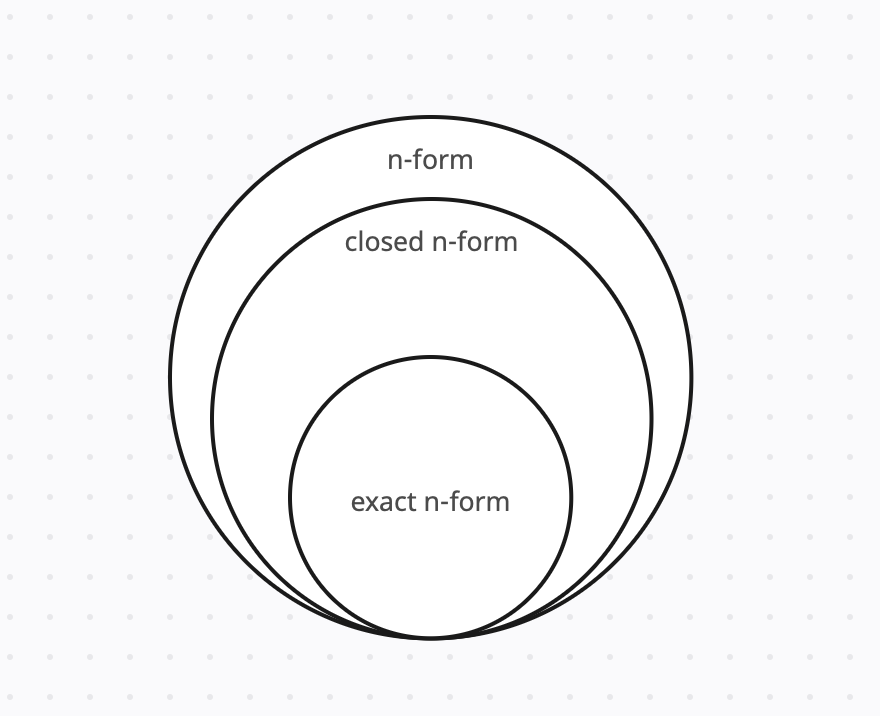
\includegraphics[height=8cm,width=14cm]{ednf}
   \end{minipage}
\end{center}
Thus, we may define the \textbf{De Rham cohomology group $H^k(M)$ in degree $k$ of  $M$} to be the quotient vector space 
\begin{align*}
H^k(M)\triangleq \frac{\set{\text{ closed $k$-th forms }}}{\set{\text{ exact $k$-th forms }}}
\end{align*}
By \myref{Theorem}{Cfz}, a 0-form is closed if and only if it is a constant, it follows from no 0-forms being exact that 
\begin{align*}
H^0(M)= \R
\end{align*}
if $M$ is connected. Note that the requirement of second countability make compact manifold have only finite amount of connected component. It follows that 
\begin{align*}
H^0(M)=\R^{\text{number  connected components of }M}
\end{align*}
It is clear that 
\begin{align*}
H^k(M)=\Omega^k(M)=0\text{ if }k>\operatorname{dim}M
\end{align*}
We may define a bilinear product $H^k(M)\times H^l(M)\to H^{k+l}(M)$ by 
\begin{align*}
[\alpha ][\beta ]\triangleq  [\alpha \wedge  \beta ]
\end{align*}
To see that this bilinear product is well-defined, compute 
\begin{align*}
  (\alpha + d\gamma )\wedge  (\beta  + d\delta)&= \alpha \wedge  \beta + \alpha \wedge  d \delta + d\gamma  \wedge  \beta  + d\gamma   \wedge  d\delta     \\
  &= \alpha \wedge  \beta  + (-1)^kd(\alpha \wedge  \delta )  + (-1)^{k-1}d (\gamma \wedge  \beta  )+d(\gamma  \wedge  d \delta )
\end{align*}
differing to $\alpha \wedge  \beta $ by some exact $k+l$-th form. If $F:M\rightarrow N$ is a smooth map, then we have a natural linear map $F^*:H^k(N)\rightarrow H^k(M)$ defined by 
\begin{align*}
F^* [\alpha ]\triangleq [F^* \alpha ]
\end{align*}
Again, this is well defined because 
\begin{align*}
F^*(\alpha +d \gamma )= F^* \alpha +d F^* \gamma  
\end{align*}
differing to $F^*\alpha $ by some exact $k$-form. 
\end{mdframed}
\begin{theorem}
\label{PPL}
\textbf{(Deformation invariance of De Rham Cohomology group)} Let $F:M\times  (-\epsilon  ,1+\epsilon )\rightarrow N$ be a smooth map. If we define $F_t:M\rightarrow N$ by 
\begin{align*}
F_t(x)\triangleq F(x,t)
\end{align*}
then for all $k\geq 0$
\begin{align*}
F_0^*=F_1^*
\end{align*}
\end{theorem}
\begin{proof}
Fix some closed form $\alpha \in \Omega^k(N)$. Locally, because $d\textbf{x}^1,\dots ,d\textbf{x}^m,dt$ form a basis for $T_p^*(M\times (-\epsilon , 1+\epsilon ) )$, by \myref{Theorem}{Boe} we may decompose $F^* \alpha $ into 
\begin{align*}
F^* \alpha  = \beta_t + \gamma_t \wedge  dt 
\end{align*}
where $\beta _t,\gamma _t\in \Omega^k (M)$. Write 
\begin{align*}
\beta _t= \sum_I B^I (\textbf{x}^1,\dots ,\textbf{x}^m,t)d\textbf{x}^I \text{ and } \gamma _t= \sum_I C^I (\textbf{x}^1,\dots ,\textbf{x}^m,t)d\textbf{x}^I
\end{align*}

Using \myref{Theorem}{Picw}, we may compute 
\begin{align*}
d(\beta _t + \gamma_t \wedge  dt )&=  d\Big( \sum_I B^I(\textbf{x}^1,\dots ,\textbf{x}^m,t)d\textbf{x}^I \Big) + d \Big(\sum_I C^I (\textbf{x}^1,\dots ,\textbf{x}^m,t)d\textbf{x}^I \Big) \wedge  dt  \\
&= \sum_I \Big[\sum_{j=1}^m \frac{ \partial B^I}{\partial \textbf{x}^j} d\textbf{x}^j \wedge    d\textbf{x}^I + \frac{\partial B^I}{\partial t}dt \wedge  d\textbf{x}^I    \Big] + \sum_I \sum_{j=1}^m \frac{\partial C^I}{\partial \textbf{x}^j}d\textbf{x}^j \wedge  d\textbf{x}^I \wedge  dt   \\
&= d_M \beta_t - \frac{\partial \beta _t}{\partial t} \wedge  dt+  (d_M \gamma_t) \wedge  dt 
\end{align*}
This with \myref{Theorem}{Pic} and the fact $\alpha $ is closed give us 
\begin{align*}
0=F^* d\alpha =dF^* \alpha = d(\beta _t + \gamma_t \wedge  dt ) =d_M\beta_t - \frac{\partial \beta _t}{\partial t}\wedge  dt + (d_M \gamma _t )\wedge  dt   
\end{align*}
This give us 
\begin{align*}
\frac{\partial \beta _t}{\partial t}= d_M \gamma_t
\end{align*}
Note that 
\begin{align*}
  F_t^* \alpha = \beta _t
\end{align*}
We then have 
\begin{align*}
  F_1^* \alpha -F_0^{*}\alpha &= \int_0^1 \frac{\partial \beta_t }{\partial t}dt \\
  &=\int_0^1 d_M \gamma_t dt =d_M \int_0^1 \gamma_t dt
\end{align*}
\end{proof}
\begin{corollary}
\label{PL}
\textbf{(Poincare Lemma)} Let $n,k\geq 1$. We have 
\begin{align*}
H^k(\R^n)=0 
\end{align*}
\end{corollary}
\begin{proof}
 Define $F:\R^n\times (-\epsilon ,1+\epsilon )\rightarrow \R^n$ by 
  \begin{align*}
  F(\textbf{x},t)\triangleq t\textbf{x}
  \end{align*}
so that 
\begin{align*}
F_0\text{ is the zero map and $F_1$ is the identity map }
\end{align*}
Now, because for $k\geq 1$
\begin{align*}
  &F_0^*:\Omega^k(\R^n)\rightarrow \Omega^k(\R^n)\text{ is a zero map } \\
  \text{ and }&F_1^* :\Omega^k(\R^n)\rightarrow \Omega^k (\R^n)\text{ is the identity map }
\end{align*}
we have 
\begin{align*}
&F_0^*:H^k(\R^n)\rightarrow H^k(\R^n)\text{ is a zero map } \\
  \text{ and }&F_1^*:H^k(\R^n)\rightarrow H^k(\R^n)\text{ is the identity map }
\end{align*}
\myref{Theorem}{PPL} states that $F_0^*=F_1^*$. It then follows that $H^k(\R^n)=0$.
\end{proof}
\begin{mdframed}
The same argument can be used to show 
\begin{align}
\label{hkm}
H^k(M\times \R^m)\cong  H^k(M)
\end{align}
for $k\geq 0$ by setting 
\begin{align*}
F(p,\textbf{x},t)\triangleq (p,t \textbf{x})
\end{align*}
\end{mdframed}
\begin{mdframed}
We now compute $H^k(S^1)$ by another method. Again note that $H^0(S^1)\cong  \R$ because $S^1$ is connected and  $H^k(S^1)\cong 0$ for $k\geq 2$ because $\operatorname{dim}S^1=1$. Recall that $S^1\cong  \R \setminus \Z$ where $\R \setminus \Z$ is given the smooth structure 
\begin{align*}
  \begin{cases}
\phi_0: \set{[x]:x\in (0,1)}  \rightarrow (0,1) \\
\phi_0 ( \pi ^{-1}(x))\triangleq x
  \end{cases} \text{ and }\begin{cases}
\phi_1: \set{[x]:x\in (\frac{-1}{2},\frac{1}{2})}  \rightarrow (-\frac{1}{2},\frac{1}{2}) \\
\phi_1 ( \pi ^{-1}(x))\triangleq x
  \end{cases}
\end{align*}
We claim the $1$-form  $\alpha \in \Omega^1 (\R \setminus \Z)$ defined by 
\begin{align*}
\alpha \triangleq \begin{cases}
  dx_0 \text{ on }\set{[x]: x \in (0,1)} \\
  dx_1\text{ on }\set{[x]:x \in (\frac{-1}{2}, \frac{1}{2})}
\end{cases}
\end{align*}
is well-defined, where $x_0: \set{[x]: x \in (0,1)}\rightarrow (0,1),x_1 : \set{[x]:x \in (\frac{-1}{2}, \frac{1}{2})}\rightarrow  (\frac{-1}{2}, \frac{1}{2})$ is defined by 
\begin{align*}
x_0\triangleq \phi_0   \text{ and }x_1 \triangleq \phi_1
\end{align*}
This is true because the area where two charts overlaps have two connected components, and $x_0,x_1$ take the same value on one of them while taking values different by constant $1$ on another. Also note that $\alpha $ is clearly non-zero, so we have shown $\Omega^1 (\R \setminus \Z)\neq 0$. \\

Note that $\alpha $ is not exact since if $\alpha = d\gamma $ for some $\gamma \in \Omega^0(\R \setminus \Z)$ then $\gamma $ on $\set{[x]: x \in (0,1)}$ must have the same action as $x_0$, which is impossible since this make  $\gamma $ discontinuous at end-point. On the other hand, suppose $\beta  \in \Omega^1 (\R \setminus \Z)$. Write in local coordinate 
\begin{align*}
\beta  (x)=g(x)dx\text{ on }\set{[x]:x \in (0,1)}
\end{align*}
Set $f\in \Omega^{1}(\R \setminus \Z)$ by 
\begin{align*}
f(x)\triangleq \int_0^x g(s)ds - \Big( \int_0^1 g(s)ds \Big)x \text{ on } \set{[x]:x \in (0,1)}
\end{align*}
It follows that 
\begin{align*}
\beta = \Big( \int_0^1 g(s)ds \Big)\alpha + df
\end{align*}
We have shown $H^1(S^1)=\R$
\end{mdframed}
\begin{theorem}
\textbf{(De Rham Cohomology of $S^n$)} For $n>0$ 
 \begin{align*}
H^k (S^n) \cong \begin{cases}
  \R & \text{ if $k=0\text{ or }n$ }\\
  0& \text{ if otherwise }
\end{cases}
\end{align*}
\end{theorem}
\begin{proof}
The case of $n=1$ have been proved in the above paragraph. We first prove 
\begin{align*}
\vi{H^1(S^2)\cong  0}
\end{align*}
Define  
 \begin{align*}
 U \triangleq S^2 \setminus \overline{B_\epsilon (N)} \text{ and }V \triangleq S^2 \setminus \overline{B_\epsilon (S)}
 \end{align*}
By means of stereographic projection, we know $U$ and  $V$ are both diffeomorphic to an open ball in  $\R$. Let $\alpha \in \Omega^1(S^2)$ be a closed $1$-form.  By \customref{PL}{Poincare Lemma}, $\alpha |_U$ and $\alpha |_V$ are both exact. Write 
\begin{align*}
\alpha = du \text{ on }U\text{ and }\alpha =dv\text{ on }V
\end{align*}
where $u\in \Omega^{0}(U),v \in \Omega^{0}(V)$ are two zero-forms. Compute 
\begin{align*}
d(u-v)=\alpha -\alpha =0\text{ on }U\cap V
\end{align*}
This implies $u-v \in \Omega^{0}(U \cap V)$ are closed. It then follows from $U \cap V$ being connected that $u-v\in \Omega^0(U \cap V)$ is constant. Therefore, if we define $\gamma \in \Omega^0(S^1)$ by 
\begin{align*}
\gamma  \triangleq \begin{cases}
  u& \text{ on  }U\\
  v+c&\text{ on }V
\end{cases}
\end{align*}
where $c\equiv u-v$ on $U \cap V$, then $\gamma $ is well-defined. It is easily seen that $\alpha = d\gamma $. $\vdone$\\

We now prove 
\begin{align*}
\blue{H^2(S^2)\cong  \R}
\end{align*}
Again, define 
 \begin{align*}
 U \triangleq S^2 \setminus \overline{B_\epsilon (N)} \text{ and }V \triangleq S^2 \setminus \overline{B_\epsilon (S)}
 \end{align*}
By means of stereographic projection, we know $U$ and  $V$ are both diffeomorphic to an open ball in  $\R^2$. Let $\alpha \in \Omega^2(S^n)$ be a closed $2$-form. By \customref{PL}{Poincare Lemma}, $\alpha |_U, \alpha |_V$ are both exact. Write 
\begin{align*}
\alpha = du \text{ on }U\text{ and }\alpha =dv\text{ on }V
\end{align*}
where $u\in \Omega^{1}(U),v \in \Omega^{1}(V)$ are two $1$-forms. Compute 
\begin{align*}
d(u-v)=\alpha -\alpha =0\text{ on }U\cap V
\end{align*}
This implies $u-v\in \Omega^{1}(U \cap V)$ are closed. Compute by \myref{Equation}{hkm} 
\begin{align*}
H^{1}(U \cap V)\cong  H^{1}(S^{1}\times \R)\cong  H^{1}(S^{1})\cong \R
\end{align*}
Let $[\omega]\in H^1(U \cap V)$ be non-trivial. We then see 
\begin{align*}
u-v=c \omega + dw 
\end{align*}
for some unique $c \inr$ and $w\in \Omega^0(U \cap V)$. We now show that \olive{such $c$ only depends on $\alpha $, independent of choice of  $u,v$}.   




We may now define a linear map $H^2(S^2)\rightarrow \R$ by 
\begin{align*}
\alpha \mapsto c_\alpha 
\end{align*}

\end{proof}
\section{Orientation}
\begin{abstract}
  This section gives an \customref{EDO}{equivalent definitions for orientation} and constructs \customref{Svf}{the standard volume form for $S^n$}. In this section, $M$ is always a $m$-dimensional smooth manifold  
\end{abstract}
\begin{mdframed}
Let $(U,\textbf{x}),(V,\textbf{y})$ be two charts for $M$. If 
\begin{align*}
  \operatorname{det} \Big(\frac{\partial \textbf{y}^i}{\partial \textbf{x}^j} \Big)>0\text{ everywhere on }U \cap V
\end{align*}
we say their transition function is \textbf{orientation preserving}. We say an atlas $\mathcal{U}$ for  $M$ is  \textbf{oriented atlas} if all transition functions for $\mathcal{U}$ is orientation preserving. A maximal oriented atlas for $M$ is said to be an  \textbf{orientation} of $M$. If $M$ admits an oriented atlas, we say  $M$ is  \textbf{orientable}; moreover, if we say $M$ is an  \textbf{oriented manifold}, we mean that $M$ is equipped with a maximal oriented atlas.\\

By a \textbf{volume form on $M$}, we mean a top-degree differential form $\omega \in \Omega^m(M)$ such that $\omega$ is non-zero everywhere. On the space of volume forms, we may define an equivalence relation by relating two volume forms $\omega,\omega'$ together if there exists some positive zero-form $f\in \Omega^0(M)$ such that  $\omega'=f \omega$.\\


We may now prove the equivalency of two definitions of orientation.  
\end{mdframed}
\begin{theorem}
\label{EDO}
\textbf{(Equivalent Definition of Orientation)} Let $M$ be a smooth manifold. There exists a one-to-one correspondence between the set of orientation of $M$ and the set of equivalence class of volume forms. 
\end{theorem}
\begin{proof}
Let $\omega$ be a volume form. By changing $\textbf{x}^1$ to $-\textbf{x}^1$ if necessary, we may find an atlas $\mathcal{U}$ such that 
\begin{align}
\label{vu}
f>0\text{ when we write }\omega= f(\textbf{x}) \ld^1 \wedge  \cdots \wedge  \ld ^n  \text{ on }U
\end{align}
for all $(U,\textbf{x})\in \mathcal{U}$. If on another chart $(V,\textbf{y})\in \mathcal{U}$, we write 
\begin{align*}
\omega= g(\textbf{y})\tilde{\ld }^1 \wedge  \cdots \wedge  \tilde{\ld }^n  \text{ on }V
\end{align*}
by \myref{Equation}{ldi}, we may compute 
\begin{align*}
f(\textbf{x})\ld ^1 \wedge  \cdots \wedge   \ld ^n=\omega&= g(\textbf{y}) \tilde{\ld } ^1 \wedge  \cdots \wedge \tilde{\ld } ^n   \\
&= g(\textbf{y}(\textbf{x})) \operatorname{det}\Big( \frac{\partial \textbf{y}^i}{\partial \textbf{x}^j} \Big) \ld ^1 \wedge  \cdots \wedge  \ld ^n  \text{ on }U\cap V
\end{align*}
It follows from $f,g$ are both positive that $\operatorname{det}\Big( \frac{\partial \textbf{y}^i}{\partial \textbf{x}^j} \Big)>0$. We have shown $\mathcal{U}$ is an oriented atlas. Direct computation with \myref{Equation}{ldi} shows that if $\omega'$ is a volume form equivalent to $\omega$, then the oriented atlas $\mathcal{U}'$ induced by the same procedure is consistent with $\mathcal{U}$. We have constructed a function  $F$ that maps the set of equivalence class of volume forms into the set of orientation of  $M$. Note that, again, direct computation with \myref{Equation}{ldi} shows that $F$ is one-to-one. \\

It remains to show $F$ is onto. Let $(U_\alpha )$ be a maximal oriented atlas, and let \customref{Smooth manifolds always admit smooth partition of unity}{$(\phi_\alpha )$ be a partition of unity subordinate to $(U_\alpha )$}. Define $\omega \in \Omega^n(M)$ by 
\begin{align*}
\omega \triangleq \sum_{\alpha } \phi_\alpha \ld ^1_\alpha \wedge  \cdots \wedge  \ld _\alpha ^n  
\end{align*}
Note that $\omega$ is well-defined because $(\phi_\alpha )$ is locally finite. Let $p \in M$. To see $\omega$ is indeed non-vanishing, let $(U_{\alpha _1},\textbf{x})$ be a chart containing $p$, and compute on an neighborhood around $p$ 
 \begin{align*}
\omega&= \sum_{\alpha :\phi_\alpha (p)>0} \phi_\alpha d\textbf{y}^1_\alpha \wedge  \cdots \wedge  d\textbf{y}^n_\alpha    \\
&= \sum_{\alpha :\phi_\alpha (p)>0} \phi_\alpha  \operatorname{det}\Big( \frac{\partial \textbf{y}^i_\alpha  }{\partial \textbf{x}^j } \Big) d\textbf{x}^1 \wedge  \cdots \wedge   d\textbf{x}^n\neq 0
\end{align*} 
This implies that $\omega$ is a volume form satisfying \myref{Equation}{vu}. In other words, $F$ maps  $[\omega]$ to $(U_\alpha )$. We have shown $F$ is indeed onto.  
\end{proof}
\begin{mdframed}
Because of \myref{Theorem}{EDO}, if $M$ is oriented with oriented atlas $\mathcal{U}$ and  $\omega$ is a volume form such that 
\begin{align*}
f>0\text{ when we write }\omega= f(\textbf{x}) \ld^1 \wedge  \cdots \wedge  \ld ^n  \text{ on }U\text{ for all }U \in \mathcal{U}
\end{align*}
we say $\omega$ is a \textbf{positively oriented volume form}. 
\end{mdframed}
\label{Svf}
\begin{Example}{\textbf{(Standard volume form of $S^n$)}}{}
\vspace{0.8cm}
Let $f:\R^{n+1}\rightarrow \R$ be a smooth map, and $M\subseteq \R^{n+1}$ be a regular level set. By \customref{Regular Level Set Theorem}{regular level set theorem}, $M$ is an embedded submanifold of $\R^{n+1}$. Let $p \in M$. Because $p$ is a regular point, we know 
\begin{align*}
\frac{\partial f}{\partial \textbf{x}^i}(p) \neq 0\text{ for some }i
\end{align*}
then by \customref{IpFT}{implicit function theorem} and uniqueness of smooth structure, we have some chart $(U,\phi)$ around $p$ such that 
\begin{align*}
\phi (\textbf{x}^1,\dots ,\textbf{x}^n)= (\textbf{x}^1,\dots , \widehat{\textbf{x}}^i,\dots ,\textbf{x}^{n+1})
\end{align*}
and 
\begin{align*}
\frac{\partial f}{\partial \textbf{x}^i}\neq 0\text{ on }U
\end{align*}
Therefore, we may define a non-vanishing $n$-form $\omega$ on $U$ by  
\begin{align}
\label{ojh}
\omega\triangleq  (-1)^i \Big(\frac{\partial f}{\partial \textbf{x}^i}\Big)^{-1}  d\textbf{x}^1\wedge \cdots  \wedge  \widehat{d \textbf{x}}^i \wedge  \cdots \wedge  d \textbf{x}^{n+1}
\end{align}
To see $\omega$ is globally well-defined, first observe that   because $f$ is constant on  $M$, globally we have 
 \begin{align}
\label{0df}
0=\sum_{k} \frac{\partial f}{\partial \textbf{x}^k}d\textbf{x}^k
\end{align}
Now, if $(V,\psi)$ is a similarly defined chart with 
\begin{align*}
\phi (\textbf{x}^1,\dots ,\textbf{x}^n)= (\textbf{x}^1,\dots ,\widehat{\textbf{x}}^j,\dots ,\textbf{x}^{n+1}) 
\end{align*}
and 
\begin{align*}
\frac{\partial f}{\partial \textbf{x}^j}\neq 0\text{ on }V
\end{align*}
such that $V \cap U\neq \varnothing$, we may compute by \myref{Equation}{0df} that 
\begin{align*}
d\textbf{x}^j = - \Big( \frac{\partial f}{\partial \textbf{x}^j} \Big)^{-1} \sum_{k\neq j} \frac{\partial f}{\partial \textbf{x}^j}  d\textbf{x}^k\text{ on }U \cap V
\end{align*}
Therefore, the expression of $\omega$ in \myref{Equation}{ojh} on $V \cap U$ is equal to 
\begin{align*}
  \omega= (-1)^j \Big( \frac{\partial f}{\partial \textbf{x}^j} \Big)^{-1}d\textbf{x}^1 \wedge  \cdots \wedge  \widehat{d \textbf{x}}^j \wedge  \cdots \wedge  d\textbf{x}^{n+1}    
\end{align*}
We have shown $\omega$ is globally well-defined. Now, if we let $f(\textbf{x})\triangleq \abso{\textbf{x}}^2$ and let $f(M)=1$, we see $M=S^n$ and  
 \begin{align*}
\omega= \frac{(-1)^i}{2\textbf{x}^i} d\textbf{x}^1 \wedge  \cdots \wedge \widehat{d \textbf{x}}^i \wedge \cdots \wedge  d\textbf{x}^{n+1}    
\end{align*}
on $\set{\textbf{x} \in S^n: \textbf{x}^i \neq 0}$. We call this $\omega$ the \textbf{standard volume form on $S^n$}. 
\end{Example}
\begin{mdframed}
Because the $m$-th exterior powers of $T_p^*M$ are 1-dimensional, for each pair of volume forms  $\omega,\omega' \in \Omega^m(M)$, there exists some $f:M\rightarrow \R^*$ such that $\omega'=f \omega$. Charts by charts, one can check that $f\in \Omega^0(M)$ is indeed smooth. Define $g:\R^*\rightarrow \set{0,1}$ by 
  \begin{align*}
  g(x)\triangleq \begin{cases}
    1& \text{ if $x>0$ }\\
    0& \text{ if $x<0$ }
  \end{cases}
  \end{align*}
Because $g$ is continuous, we know  $g \circ f: M\rightarrow \set{0,1}$ is continuous. It then follows that if $M$ has  $n$ connected components, then there are $2^n$ orientation on  $M$. 
\end{mdframed}
\section{Integration on Manifold}
\begin{abstract}
In this section, we introduce the idea of integration on smooth manifold and prove  \customref{HBT}{the hairy ball theorem} for smooth vector field and that \customref{rpin}{$\RP^n$ is not orientable for even  $n$}
\end{abstract}
\begin{mdframed}
Let $M$ be an oriented manifold and  $\omega \in \Omega^m(M)$ be a top-degree form with compact support.  Because $M$ is oriented and $\omega$ is of compact support, we may find a finite set of charts $U_1,\dots ,U_N$ such that $\operatorname{supp}\omega \subseteq U_1 \cup \cdots \cup U_N$ and $f_i$ share the same sign if we write on each chart  
\begin{align*}
\omega|_{U_i }= f_i (\textbf{x})\ld_i^1 \wedge  \cdots \wedge  \ld_i^m
\end{align*}
Let $\phi_1,\dots ,\phi_N$ be a smooth partition of unity subordinated to $U_1,\dots ,U_N$. We define the integral of $\omega$ on $M$ to be 
 \begin{align*}
\int_M \omega\triangleq \sum_{i=1}^N \int_{\R^m} \phi_i f_i (\textbf{x}) 
\end{align*}
To show that the definition is independent of choice of the finite covers and partition of unity, let $\tilde{U}_j$ be a another finite cover and $\tilde{\phi}_j$ a subordinating partition of unity, and check 
\begin{align*}
\sum_j \int_M \tilde{\phi}_j \omega= \sum_{i,j} \int_M \tilde{\phi}_j \phi_i \omega  = \sum_i \int_M \phi_i \omega
\end{align*}
\end{mdframed}
\begin{theorem}
\label{SCST}
\textbf{(Special Case of Stoke's Theorem)} Let $M$ be oriented and  $\omega\in \Omega^{m-1}(M)$ be of compact support. We have 
\begin{align*}
\int_M d\omega=0
\end{align*}
\end{theorem}
\begin{proof}
Again, let $\phi_i$ be a partition of unity subordinated to a positively oriented finite set of charts. On each chart, we may write 
\begin{align*}
\phi_i \omega= \sum_{n=1}^m (-1)^{n+1} a_n \ld^1 \wedge  \cdots \wedge \widehat{\ld }^n \wedge  \cdots \wedge \ld^m    
\end{align*}
Compute 
\begin{align*}
d(\phi_i \omega)= \sum_{n=1}^m \frac{\partial a_n}{\partial \textbf{x}^n} \ld ^1 \wedge  \cdots \wedge \ld^m   
\end{align*}
It then follows from each $a_n$ is of compact support that 
 \begin{align*}
\int_M d\omega= \sum_i \int_M d(\phi_i \omega)=0
\end{align*}
\end{proof}
\begin{mdframed}
Immediately, following from \customref{SCST}{special case of Stoke's theorem}, we see that if $M$ is compact and orientable, then 
 \begin{align*}
H^m(M)\neq 0
\end{align*}
since if $\alpha \in \Omega^m(M)$ is a positively oriented volume forms, then 
\begin{align*}
\int_M \alpha  >0
\end{align*}
which implies $\alpha $ is not exact. 
\end{mdframed}
\begin{theorem}
\label{rpin}
\textbf{($\RP^n$ is not orientable for even  $n$)} Define an equivalence relation on $\R^{n+1}\setminus \set{\textbf{0}}$ by 
\begin{align*}
\textbf{x}\sim \textbf{y}\text{ if }\textbf{x}=\ld  \textbf{y}\text{ for some }\ld \inr
\end{align*}
Let $\pi $ be the quotient map and $\RP^n$ be the quotient space. If we give $\RP^n$ the atlas 
\begin{align*}
[\textbf{x}_1 ,\dots ,\textbf{x}_{n+1}]\mapsto  \Big(\frac{\textbf{x}_1}{\textbf{x}_i}, \dots , \frac{\textbf{x}_{i-1}}{\textbf{x}_i},\frac{\textbf{x}_{i+1}}{\textbf{x}_i}, \dots ,\frac{\textbf{x}^{n+1}}{\textbf{x}^i}\Big) 
\end{align*}
and $n$ is even, then  $\RP^n$ is not orientable. 
\end{theorem}
\begin{proof}
We first show that
\begin{center}
   \begin{minipage}{0.9\linewidth}  
     \olive{$\pi  : S^n \rightarrow \RP^n $ is a smooth immersion}. 
   \end{minipage}
\end{center}
Define $U\triangleq \set{\textbf{x}\in S^n: \textbf{x}_1>0}$ and $\phi : U\rightarrow \R^n$ by 
\begin{align*}
\phi (\textbf{x})\triangleq (\textbf{x}_2 ,\dots , \textbf{x}_n)
\end{align*}
Compute 
\begin{align*}
\psi \circ \pi  \circ  \phi ^{-1} (\textbf{x}_2 ,\dots ,\textbf{x}_{n+1})=  \Big(\frac{\textbf{x}_2}{\textbf{x}_1},\dots , \frac{\textbf{x}_{n+1}}{\textbf{x}_1}\Big)
\end{align*}
We have shown $\pi $ is indeed smooth. To see $\pi _{*,p}$ is invertible everywhere, observe that $\psi \circ \pi  \circ   \phi^{-1}$ have the action 
\begin{align*}
\textbf{y}\mapsto  \frac{\textbf{y}}{\sqrt{1- \abso{\textbf{y}}^2} }
\end{align*}
which has a left inverse 
\begin{align*}
\textbf{y}\mapsto \frac{\textbf{y}}{\sqrt{1+ \abso{\textbf{y}}^2} }
\end{align*}
One can check from definition of $\pi $ that this left inverse is indeed an inverse. More precisely, we have established a diffeomorphism between $U$ and $\pi  (U)$. Therefore, $\pi$ is a local diffeomorphism. This implies $\pi _{*,p}$ is invertible everywhere. $\odone$ \\

 Let $\omega \in \Omega^n (S^n)$ be the \customref{Svf}{standard volume form of $S^n$}. Define a smooth diffeomorphism $\sigma :S^n\rightarrow S^n$ by 
\begin{align*}
\sigma (\textbf{x})\triangleq - \textbf{x}
\end{align*}
We now show 
\begin{align}
\label{sgw}
  \vi{\sigma^* \omega = - \omega}
\end{align}
Compute on $\set{\textbf{x} \in S^n : \textbf{x}_i \neq 0} $
\begin{align*}
  \sigma^* \omega &=  \sigma^*  \Big[\frac{(-1)^i}{2\textbf{x}_i} d\textbf{x}_1 \wedge  \cdots \wedge \widehat{d \textbf{x}_i} \wedge \cdots \wedge  d\textbf{x}_{n+1}  \Big] \\
  &= \frac{(-1)^i}{-2\textbf{x}_i}d(-\textbf{x}_1)\wedge  \cdots \wedge  d(-\textbf{x}_{i-1}) \wedge  d(-\textbf{x}_{i+1}) \wedge  \cdots \wedge   d(-\textbf{x}_{n+1})    \\
  &=(-1)^{n-1} \omega=-\omega 
\end{align*}
Repeating the same computation on $\textbf{x}_j \neq 0$, we see that, indeed, $\sigma^* \omega= -\omega$ globally. $\vdone$\\


\As{$\theta \in \Omega^n (\RP^n)$ is a volume form}. Because $\pi$ is an immersion, we know $\pi ^* \theta \in \Omega^n (S^n)$ is also a volume form. Therefore, we may define an no-where-zero $f\in \Omega^0(S^n)$ by 
\begin{align*}
f\triangleq \frac{\pi ^* \theta}{\omega }
\end{align*}
It is clear that $\pi \circ \sigma= \pi  $. Therefore, 
\begin{align*}
  f\omega= \pi ^* \theta= (\pi  \circ  \sigma)^* \theta= \sigma^* \pi ^* \theta= \sigma^* (f \omega)= -(f \circ \sigma)\omega 
\end{align*}
This give us 
\begin{align*}
f(\textbf{x})=-f(-\textbf{x})\text{ for all }\textbf{x}\in S^n
\end{align*}
This is impossible, since the fact that $S^n$ is connected implies  $f$ have the same sign everywhere. \CaC 
\end{proof}
\begin{theorem}
\label{HBT}
\textbf{(Hairy Ball Theorem in Differential Geometry)} Let  $X\in \mathfrak{X}(S^{2m})$ be a smooth vector field. 
\begin{align*}
\text{ There exists some $p  \in S^{2m}$ such that }X_p=0
\end{align*}
\end{theorem}
\begin{proof}
\As{$X$ is non-vanishing}. Obviously, we may identify each $T_\textbf{x}S^{2m}$ as a $2m$-dimensional subspace of  $\R^{2m+1}$ orthogonal to $\textbf{x}$. This way, $X$ is smooth function that maps  $S^{2m}$ into $\R^{2m+1}$ such that 
\begin{align*}
X(\textbf{x})\cdot \textbf{x}=0\text{ for all }\textbf{x} \in S^{2m}
\end{align*}
Because the normalizing function $\textbf{x}\mapsto \frac{\textbf{x}}{\abso{\textbf{x}}}$ is smooth, if we define $\widehat{X}\in \mathfrak{X}(S^{2m})$ by 
\begin{align*}
\widehat{X}_\textbf{x}\triangleq \frac{X_\textbf{x}}{\abso{X_\textbf{x}}}
\end{align*}
then $\widehat{X}$ is indeed smooth. Define $F_t:S^{2m}\rightarrow S^{2m}$ by 
\begin{align*}
F_t(\textbf{x})\triangleq (\cos t)\textbf{x}+ (\sin t)\widehat{X}_\textbf{x}
\end{align*}
Tedious computations shows that $F:S^{2m}\times \R \rightarrow S^{2m}$ is indeed smooth. Compute 
\begin{align*}
F_0(\textbf{x})=\textbf{x}\text{ and }F_\pi  (\textbf{x})=-\textbf{x}\text{ for all }\textbf{x}\in S^{2m}
\end{align*}
Let $\omega \in \Omega^{2m}(S^{2m})$ be the \customref{Svf}{standard volume form}. By \myref{Equation}{sgw} proved in \myref{Theorem}{rpin}, we have 
\begin{align*}
F_0(\omega)=\omega\text{ and }F_\pi  (\omega)=-\omega
\end{align*}
It then follows from \customref{PPL}{deformation invariance of De Rham cohomology group} that $\omega$ is exact. This cause a contradiction, since \customref{SCST}{special case of Stoke's theorem} says that exact top-form $\omega$ on $S^{2n}$, which is compact, must have 
\begin{align*}
\int_M \omega =0
\end{align*}
while the fact $\omega$ is the standard volume form implies 
\begin{align*}
\int_M \omega> 0 \tCaC
\end{align*}
\end{proof}
\section{Stoke's Theorem}
\begin{abstract}

\end{abstract}
\begin{mdframed}
In this section, we use  $\H^n$ to denote the upper-half space of $\R^n$
\begin{align*}
\H^n \triangleq \set{\textbf{x}\in \R^n: \textbf{x}^n \geq 0}
\end{align*}
By a $n$-dimensional topological manifold with boundary, we mean a second-countable and Hausdorff topological space $M$ such that for all $p \in M$, there exists some neighborhood $U$ around  $p$ homeomorphic to some open subsets of  $\H^n$. By invariance of domain, a non-trivial Theorem in algebraic topology, one can deduce that if $p$ is mapped by some chart into $\partial \H^n$, then all charts map $p$ into  $\partial \H^n$. Therefore, we may distinguish between the \textbf{interior $M^\circ $ and boundary $\partial M$ of $M$}.  \\

It is clear that $M^\circ $ and $\partial M$ when endowed with subspace topology from $M$, they are respectively a $n$-dimensional topological  manifold and a $(n-1)$-dimensional topological manifold. Let $f$ be a function that maps $E\subseteq \H^n$ into $\R^n$, where $E$ is open in  $\H^n$ and contain $p \in \partial \H^n$, we say $f$ is smooth at $p$ if there exists some smooth function $\widehat{f}:B_\epsilon (p)\rightarrow \R^n$ such that 
\begin{align*}
\widehat{f}\equiv f \text{ on }E\cap B_\epsilon (p)
\end{align*}
With this in mind, it make sense for us to talk about \textbf{smooth manifold with boundary}. \\

Let $p \in \partial M$ and $(U,\phi)$ be a chart around $p$. Because
\begin{align*}
T_pM\cong  T_p U\cong  T_{\phi (p)}\phi (U)\cong  T_{\phi (p)} \H^n \cong  T_{\phi (p)}\R^n
\end{align*}
we see $T_pM$ is also  $n$-dimensional, where the last isomorphism is given by the derivative of inclusion map $\diota: \H^n\rightarrow \R^n $. (Lemma 3.11 in Lee) 
\end{mdframed}
\begin{theorem}
\textbf{(Induced orientation on boundary)} If $\mathcal{U}$ is an oriented atlas for $M$, then its restriction 
\begin{align*}
\mathcal{U}'\triangleq \bset{(U\cap \partial M,\phi |_{U \cap \partial M}): (U,\phi) \in \mathcal{U}}
\end{align*}
is an oriented atlas for $\partial M$. 
\end{theorem}
\begin{proof}
Let $(U,\textbf{x}),(V,\textbf{y}) \in \mathcal{U}$. Because 
\begin{align*}
\textbf{y}^n (\textbf{x}^1,\dots ,\textbf{x}^{n-1},0)=0
\end{align*}
we know 
 \begin{align*}
\frac{\partial \textbf{y}^n}{\partial \textbf{x}^{i}}=0,\frac{\partial \textbf{y}^n}{\partial \textbf{x}^n}>0\text{ for $i<n$ on }\partial M
\end{align*}
Then because the Jacobian $J_M$ of the transition function between $\textbf{x},\textbf{y}$ has the form 
\begin{align*}
\begin{vmatrix} 
  \frac{\partial \textbf{y}^1}{\partial \textbf{x}^1} & \cdots & \frac{\partial \textbf{y}^1}{\partial \textbf{x}^{n-1} & \frac{\partial \textbf{y}^1}{\partial \textbf{x}^n}} \\
  \vdots & \ddots & \vdots & \vdots  \\
  \frac{\partial \textbf{y}^{n-1}}{\partial \textbf{x}^1} & \cdots & \frac{\partial \textbf{y}^{n-1}}{\partial \textbf{x}^{n-1}} & \frac{\partial \textbf{y}^{n-1}}{\partial \textbf{x}^n} \\
  0 & \cdots & 0 & \frac{\partial \textbf{y}^n}{\partial \textbf{x}^n}
\end{vmatrix}\text{ on }\partial M
\end{align*}
we see that the Jacobian $J_{\partial M}$ of the transition function between the restricted $\textbf{x},\textbf{y}$ is 
\begin{align*}
\begin{vmatrix} 
  \frac{\partial \textbf{y}^1}{\partial \textbf{x}^1} & \cdots & \frac{\partial \textbf{y}^1}{\partial \textbf{x}^{n-1}} \\ 
  \vdots & \ddots & \vdots  \\
  \frac{\partial \textbf{y}^{n-1}}{\partial \textbf{x}^1} & \cdots & \frac{\partial \textbf{y}^{n-1}}{\partial \textbf{x}^{n-1}}  
\end{vmatrix} = \frac{J_M}{\frac{\partial \textbf{y}^n}{\partial \textbf{x}^n}}>0
\end{align*}
\end{proof}
\begin{mdframed}
Note that if a positively oriented volume form $\omega$ has the expression 
\begin{align*}
f(\textbf{x}) d\textbf{x}^1 \wedge  \cdots \wedge  d\textbf{x}^n  
\end{align*}
then its pullback $\diota^*\omega $ to the boundary by \textbf{stoke convention} have the expression 
\begin{align}
\label{-1n}
  (-1)^n f(\textbf{x})d\textbf{x}^1 \wedge  \cdots \wedge  d\textbf{x}^{n-1}  
\end{align}
\end{mdframed}
\begin{theorem}
\textbf{(Stoke's Theorem)} Let $M$ be an oriented  $n$-dimensional manifold with  boundary $\partial M$, and let $\omega \in \Omega^{n-1}(M)$ be of compact support. We have 
\begin{align*}
\int_M d\omega = \int_{\partial M} \omega 
\end{align*}
where the restriction of $\omega$ on $\partial M$ should be considered as the pullback $\diota^*\omega $ of $\diota: \partial M\rightarrow M $. 
\end{theorem}
\begin{proof}
Let $\set{U_\alpha }$ be an open cover, and let $\set{\rho_\alpha }$ be a subordinate partition of unity. Therefore, we may write 
\begin{align*}
\int_M d\omega= \sum_{i=1}^N \int_M \rho_i d\omega= \sum_{i=1}^N \int_M d(\rho_i \omega)
\end{align*}
Fix $i$. Write   
\begin{align}
\label{fi}
\rho_i \omega= \sum_{j=1}^n (-1)^{j-1}a_j d\textbf{x}^1 \wedge  \cdots \wedge  \widehat{d \textbf{x}^j}  \wedge  \cdots \wedge   d\textbf{x}^n 
\end{align}
And compute 
\begin{align*}
d (\rho_i \omega)= \sum_{j=1}^n \frac{\partial a_j}{\partial \textbf{x}^j} d\textbf{x}^1 \wedge  \cdots \wedge  d\textbf{x}^n  
\end{align*}
If $U_i\cap  \partial M= \varnothing$, then we may use Fubini's Theorem and Fundamental Theorem of Calculus to conclude 
\begin{align*}
\int_M d(\rho_i \omega)=0 
\end{align*}
If  $U_i \cap \partial M \neq \varnothing$,  by \myref{Equation}{-1n} and \myref{Equation}{fi}, we may observe 
\begin{align*}
\diota^* (\rho_i \omega) = - a_n d\textbf{x}^1 \wedge  \cdots \wedge  d\textbf{x}^{n-1}  
\end{align*}
And again use Fubini's Theorem and Fundamental Theorem of Calculus to compute 
\begin{align*}
\int_M d(\rho_i \omega)=  \int_{\textbf{x}^n \geq 0} \frac{\partial a_n}{\partial \textbf{x}^n} &= \int_{\R^{n-1}} a_n(\textbf{x}^1,\dots ,\textbf{x}^n)\Big|_{\textbf{x}^n=0}^{\infty } \\
&=-\int_{\R^{n-1}} a_n (\textbf{x}^1,\dots ,\textbf{x}^{n-1},0) \\
&=\int_{\partial M} \rho_i \omega
\end{align*}
This finishes the proof.
\end{proof}
\begin{theorem}
\textbf{(Brouwer's fixed point Theorem)} If 
\end{theorem}
\begin{proof}

\end{proof}
\begin{theorem}
\textbf{(Top De Rham cohomology group of oriented compact connected manifold)} If $M$ is a $n$-dimensional oriented compact connected manifold, then 
 \begin{align*}
H^n(M)\cong  \R
\end{align*}
\end{theorem}
\begin{proof}

\end{proof}
\section{Degree Theory}
\begin{theorem}
\textbf{(Degree of a Smooth Map)} Suppose $M$ and  $N$ are compact, connected, oriented, smooth manifold of dimension  $n$, and  $F:M\rightarrow N$ is a smooth map. There exists a unique integer $k$, called the  \textbf{degree of $F$}, that satisfies both the following conditions 
\begin{enumerate}[label=(\alph*)]
  \item For every smooth $n$-form  $\omega$ on $N$, 
     \begin{align*}
    \int_M F^* \omega= k \int_N \omega
    \end{align*} 
  \item If $q \in N$ is a regular value of $F$, then 
     \begin{align*}
    k= \sum_{p \in F^{-1}(q)}\operatorname{sgn}(p)
    \end{align*}
  where $\operatorname{sgn}(p)=\operatorname{sgn}(\operatorname{det}F_{*,p})$. 
\end{enumerate}
\end{theorem}
\begin{proof}
Let $\theta$ be some $n$-from on  $N$ such that 
 \begin{align*}
\int_N \theta =1
\end{align*}
Define 
\begin{align*}
k\triangleq \int_M F^* \theta\inr
\end{align*}
Fix $\omega \in \Omega^n (N)$. Because $N$ is compact connected oriented, we know  $H^n(N)=0$. This implies 
\begin{align*}
\omega= a \theta  + \beta 
\end{align*}
for some closed $n$-form  $\beta $ on $N$. Because $M,N$ have no  boundary, and pullback maps closed forms to closed forms, we know 
\begin{align*}
\int_M F^* \omega= a\int_M F^* \theta =  k a= k \int_N \omega
\end{align*}
It remains to show $k$ satisfy condition  (b). 
\end{proof}
\chapter{Geometry Archived}
\section{Lie Group}
\begin{mdframed}
Suppose $\beta  \in \Omega^1 (\R \setminus \Z)$. Write in local coordinate 
\begin{align*}
\beta  (x)=g(x)dx\text{ on }\set{[x]:x \in (0,1)}
\end{align*}
The whole point here is then to find some $f \in \Omega^1 (\R \setminus \Z)$ so that on the chart $\set{[x]: x \in (0,1)}$, we have 
\begin{align*}
\beta = cdx + df\text{ for some constant $c$ }
\end{align*}
The argument presented in class is to set  
\begin{align*}
f(x)\triangleq \int_0^x g(s)ds\text{ for }x\in (0,1)
\end{align*}
in local coordinate and get the conclusion $c= \int_0^1 g(s)ds$. This confuse me: If $f$ have the above action on  $\set{[x]:x \in (0,1)}$, then we must have $\int_0^1 g(s)ds=0$ so that $f$ is continuous. Yet, we don't know nothing about $g$. Why can we assume $\int_0^1 g(s)ds=0$? Doesn't this assumption just make $\beta =df$ on $\set{[x]: x\in (0,1)}$?  
\end{mdframed}
\begin{mdframed}
By a \textbf{Lie group}, we mean a smooth manifold equipped with a group structure such that the inversion and group addition are both smooth map, or equivalently, that 
\begin{align*}
M^2\rightarrow  M; (g,h)\mapsto gh^{-1}
\end{align*}
is smooth. 
\end{mdframed}
\section{Integral Curve and Flow}
\begin{abstract}
Note that in this section, $I,J$ always stand for open intervals and integral is always defined on some open interval. 
\end{abstract}
\begin{mdframed}
Given some smooth manifold $M$, and some smooth map $\theta :\R \times M\rightarrow M$, we say $\theta$ is a \textbf{smooth global flow}, or an \textbf{1-parameter group of diffeomorphism}, if when we define for all $t\inr$ a function $\theta_t:M\rightarrow M$ by
\begin{align*}
\theta_t(p)\triangleq \theta (t,p)
\end{align*}
we have the following properties 
\begin{enumerate}[label=(\roman*)]
  \item $\theta_t:M\rightarrow M$ is smooth diffeomorphism for all $t\inr$. 
  \item $\theta_0=\textbf{id}$. 
  \item For all $t,s \inr,\theta_{t+s}=\theta_t \circ \theta_s$. 
\end{enumerate}
Immediately we see where does the name 1-parameter group of diffeomorphism comes from: The set  $\set{\theta_t: t\inr}$ clearly form a group with function composition. Moreover, we see that for each $p\in  M$, $\theta_t(p)$, when treated as a function in $t$, is a smooth curve in $M$, since we have the following commutative diagram 
% https://q.uiver.app/#q=WzAsMyxbMCwwLCJcXG1hdGhiYntSfVxcdGltZXMgTSJdLFsyLDAsIk0iXSxbMCwyLCJcXG1hdGhiYntSfSJdLFswLDEsIlxcdGhldGEiXSxbMiwwLCJGIl0sWzIsMSwiXFx0aGV0YV90KHApIiwyXV0=
\[\begin{tikzcd}
	{\mathbb{R}\times M} && M \\
	\\
	{\mathbb{R}}
	\arrow["\theta", from=1-1, to=1-3]
	\arrow["F", from=3-1, to=1-1]
	\arrow["{\theta_t(p)}"', from=3-1, to=1-3]
\end{tikzcd}\]
where $F(t)\triangleq (t,p)$. With this fact in mind and some tedious effort, we can induce a vector field $X$ by defining 
\begin{align}
\label{indf}
X_pf\triangleq \frac{df(\theta_t(p))}{dt}\Big|_{t=0}
\end{align}
To see $X$ is smooth, we see that if we write locally  
\begin{align*}
\theta_t(\textbf{x})=(\textbf{y}^1(t,\textbf{x}),\dots ,\textbf{y}^n(t,\textbf{x}))
\end{align*}
by \customref{CR}{Chain Rule} we have
\begin{align*}
X_{\textbf{x}}f&= \frac{\partial f(\textbf{y}^1(t,\textbf{x}),\dots ,\textbf{y}^n(t,\textbf{x}))}{\partial t}\Big|_{t=0}\\
&= \sum_{i=1}^n \frac{\partial f}{\partial \textbf{y}^i}(\textbf{x}) \frac{\partial \textbf{y}^i}{\partial t}(t,\textbf{x})\Big|_{t=0}
\end{align*}
This then give us 
\begin{align*}
Xf(\textbf{x})= \sum  \frac{\partial \textbf{y}^i}{\partial t}(0,\textbf{x}) \frac{\partial f}{\partial \textbf{y}^i} 
\end{align*}
It follows from $\textbf{y}$ being smooth that $Xf$ is smooth. We have shown smooth global flow induce smooth vector field by means of \myref{Equation}{indf}. We now show that on compact manifold, we can conversely induce smooth global flow from smooth vector filed.\\

If we say  $\gamma :I\rightarrow M$ is an \textbf{integral curve with respect to some vector field $X$}, we mean that $\gamma '(t)=X_{\gamma (t)}$ for all $t \in I$, and if we say $\gamma $ centers $p$, we mean  $0 \in I$ and $\gamma (0)=p$. Immediately, we see from \customref{Picard-Lindelof Theorem}{Picard-Lindelof Theorem} that for all $p$, there always exists some integral curve centering  $p$. Moreover, given two integral curve $\gamma_1,\gamma_2:I_1,I_2\rightarrow M$ centering $p$, if we let  $J\triangleq I_1\cap I_2$ and 
\begin{align*}
S\triangleq \set{t \in J:\gamma _1(t)=\gamma_2(t)}
\end{align*}
By continuity we see $S$ is closed in  $J$, and by \customref{Picard-Lindelof Theorem}{Picard-Lindelof Theorem} we see $S$ is also open in $I$. It then follows from  $J$ being also an open interval that  $S=J$. In other words,  $\gamma_1,\gamma _2$ agree on $J$. This then implies the existence of some integral curve $\gamma:I\rightarrow M$ centering $p$ such that every integral curve $\gamma_1:I_1\rightarrow M$ centering $p$ satisfy  $I_1 \subseteq I$ and 
\begin{align*}
\gamma (t)=\gamma_1(t)\text{ for all }t\in I_1
\end{align*}
We call this curve the \textbf{maximal integral curve centering $p$}. 
\end{mdframed}
\begin{theorem}
\textbf{(Smooth vector field induce smooth global flow on smooth compact manifold)} If $M$ is compact and  $X \in \mathfrak{X}(M)$, then for each $p\in  M$, the maximal integral curve centering $p$ is defined on the whole  $\R$ and if we define $\theta:\R\times M\rightarrow M$ by 
\begin{align*}
\theta (t,p)\triangleq \alpha _p(t)\text{ where }\alpha _p\text{ is the maximal integral curve centering $p$ }
\end{align*}
then $\theta$ form a smooth global flow.
\end{theorem}
\begin{proof}
Let $\alpha_p:I_p\rightarrow M$ be the maximal integral curve centering $p$. Our definition for $\theta$ is now only on 
\begin{align*}
\bigcup_{p\in M} I_p \times \set{p}\subseteq \R\times M
\end{align*}
Let $I_p$ be the domain of the maximal integral curve centering $p$. Clearly, for all $p \in M$ there exists some open set $U_p$ containing $\phi(I_p,p)$. Because $M$ is compact, we may select some finite open cover $U_{p_1},\dots ,U_{p_N}$. Define 
\begin{align*}
I\triangleq \bigcap_{i=1}^N I_{p_i}
\end{align*}
It is clear that $0 \in I$. It then follows that $I$ is an non-empty open interval. 






Now observe that for all $s\in I_p$ if we let 
\begin{align*}
I\triangleq \set{t\inr:t+s \in I_p}
\end{align*}
and define $\gamma :I\rightarrow M$ by 
\begin{align*}
\gamma (t)\triangleq \theta_{t+s}(p)
\end{align*}
then $\gamma $ is an integral curve centering $\theta_s(p)$. This implies $I \subseteq I_{\theta (s,p)}$ and 
\begin{align*}
\theta_t \circ \theta_s (p)=\theta_{t+s}(p)\text{ for all }t \in I
\end{align*}
\end{proof}
\begin{mdframed}
Now, suppose $\theta$ is a smooth global flow induced by smooth vector field $X$. Given some scalar function $f \in C^{\infty}(M)$, we see that if we define the \textbf{Lie derivative $\mathcal{L}_Xf\inC^{\infty}(M)$ of $f$ with respect to  $X$} by 
\begin{align*}
\mathcal{L}_Xf(p)\triangleq \frac{d}{dt}\Big|_{t=0}(f\circ \theta_t)(p)
\end{align*}
we have 
\begin{align*}
\mathcal{L}_Xf(p)&=(f\circ \alpha )'(0)\text{ where }\alpha (t)\triangleq \theta_t(p)\\
&=\alpha '(0)f \\
&=X_pf
\end{align*}
In other words, 
\begin{align*}
\mathcal{L}_Xf=Xf
\end{align*}
Given some tangent vector valued function, i.e., some smooth vector filed $Y \in \mathfrak{X}(M)$, we can similarly define the \textbf{Lie derivative $\mathcal{L}_XY\in \mathfrak{X}(M)$ of $Y$ with respect to  $X$} by 
\begin{align*}
  (\mathcal{L}_XY)_pf\triangleq \lim_{t\to 0} \frac{(\theta_{-t})_{*,\theta_t(p)}(Y_{\theta_t(p)})f-Y_pf}{t} 
\end{align*}
We shall prove that $\mathcal{L}_XY$ is well defined. 



\end{mdframed}
\begin{theorem}
\textbf{(Existence of Lie derivative)} If $X,Y\in \mathfrak{X}(M)$, then 
 \begin{align*}
\mathcal{L}_XY=[X,Y]
\end{align*}
\end{theorem}
\begin{proof}
We first define \textbf{pushforward $\widehat{Y}_t \in \mathfrak{X}(M)$} of $Y$ for all $t\inr$ by \customref{SVFP}{letting $\widehat{Y}_t$ to be the unique smooth vector field on $M$ so that  $\widehat{Y}_t,Y$ is $\theta_{t}$-related, or equivalently,  $Y,\widehat{Y}_t$ is $\theta_{-t}$-related}. Explicitly, we may write 
\begin{align*}
  Y_{\theta_t(p)}=(\theta_t)_{*,p}(\widehat{Y}_t)_p
\end{align*}
We can now rewrite 
\begin{align*}
(\mathcal{L}_XY)_pf&= \lim_{t\to 0} \frac{(\theta_{-t})_{*,\theta_t(p)}(Y_{\theta_t(p)})f-Y_pf}{t} \\
&= \lim_{t\to 0} \frac{(\widehat{Y}_t)_pf-Y_pf}{t} \\
&=\lim_{t\to 0} \frac{(\widehat{Y}_t-\widehat{Y}_0)_pf}{t} 
\end{align*}



Using \myref{Theorem}{Cfr}, we may compute, for all $p\in M$, 
\begin{align*}
\frac{d }{dt}\Big|_{t=0}(\widehat{Y}_t)(f\circ \theta_t)(p)= \frac{d }{d t}\Big|_{t=0}Yf\circ \theta_t (p)=X_p(Yf)
\end{align*}
On the other hands, we may also compute with some limit argument that  
\begin{align*}
  \frac{d}{dt}\Big|_{t=0}(\widehat{Y}_t)(f\circ \theta_t)(p)&=\lim_{t\to 0} \frac{(\widehat{Y}_t)(f\circ \theta_t)(p)-(\widehat{Y}_0)(f\circ \theta_t)(p)+(\widehat{Y}_0)(f\circ \theta_t)(p)-(\widehat{Y}_0)(f\circ \theta_0)(p)}{t}\\
&=\lim_{t\to 0}  \frac{(\widehat{Y}_t-\widehat{Y}_0)_p(f\circ \theta_t)}{t} + \lim_{t\to 0} \frac{Y_p(f\circ \theta_t)-Y_p(f\circ \theta_0)}{t} \\
&=(\mathcal{L}_XY)_pf+ \lim_{t\to 0} \frac{Y_p(f\circ \theta_t-f)}{t} \\
&=(\mathcal{L}_XY)_pf+ Y_p(\lim_{t\to 0} \frac{(f\circ \theta_t-f)}{t}) \\
&= (\mathcal{L}_XY)_pf+ Y_p(Xf)
\end{align*}
We have deduced
\begin{align*}
  (\mathcal{L}_XY)_pf+Y_p(Xf)=X_p(Yf)
\end{align*}
which is just 
\begin{align*}
\mathcal{L}_XY=[X,Y]
\end{align*}
\end{proof}
\section{Archived}
\begin{theorem}
\textbf{(Existence of Exterior Derivative)} On any smooth manifold $M$, there exists a natural linear map  $d:\Omega^k(M)\rightarrow \Omega^{k+1}(M)$ called the \textbf{exterior derivative} satisfying 
\begin{enumerate}[label=(\alph*)]
  \item If $f \in \Omega^0(M)$, then $df\in \Omega^1(M)$ is the differential of $f$. 
  \item $d^2=0$.
  \item  $d (\alpha \wedge  \beta  )=d\alpha \wedge  \beta +(-1)^k \alpha \wedge  d\beta   $ if $ \alpha  \in \Omega^k(M)$
\end{enumerate}
\end{theorem}
\begin{proof}
  Fix $\alpha  \in \Omega^k(M)$. The uniqueness part follows from computing 
  \begin{align*}
  d\alpha =\sum_I d\alpha^I \wedge  d\textbf{x}^I 
  \end{align*}
by property (b) and (c) on all charts, where 
\begin{align*}
\alpha = \sum_I \alpha^I d\textbf{x}^I
\end{align*}
We claim 
\begin{align*}
&d\alpha (X_1,\dots ,X_{k+1})\\
&\triangleq \sum_{1\leq i\leq k+1}(-1)^{i+1}X_i \Big(\omega (X_1,\dots ,\widehat{X}_i,\dots ,X_{k+1}) \Big) \\
&+\sum_{1\leq i<j\leq k+1}\omega \Big( [X_i,X_j],X_1 ,\dots ,\widehat{X}_i,\dots ,\widehat{X}_j,\dots ,X_{k+1} \Big)
\end{align*}
suffices, where the hats indicate omitted arguments.  


Let $U$ be a chart. It is then clear that we must define 
\begin{align*}
d\alpha = \sum_I d\alpha^I \wedge   d\textbf{x}^I \text{ on }U
\end{align*}
It remains to show such definition is well defined and satisfies properties (b) and (c). The well-defined part requires us to show 
\begin{align*}
\sum_I d\alpha^I d\textbf{x}^I= \sum_I d\beta^I d\textbf{y}^I 
\end{align*}
on where they overlaps. 



On $\widehat{U}\triangleq \phi^{-1}(B_{r}(\phi (p)))$, we may then write 
\begin{align*}
\alpha  = \sum_{i_1 < \cdots <i_k} a_{i_1,\dots ,i_k} d\textbf{x}^{i_1} \wedge  \cdots \wedge  d\textbf{x}^{i_k}  
\end{align*}
We define 
\begin{align*}
d\alpha \triangleq  \sum_{i_1< \cdots < i_k}da_{i_1,\dots ,i_k} \wedge   d\textbf{x}^{i_1}\wedge  \cdots \wedge  d\textbf{x}^{i_k}  \text{ on }\widehat{U}
\end{align*}
where 
\begin{align*}
da_{i_1,\dots ,i_k} X_q\triangleq \widehat{X}_q (a_{i_1,\dots ,i_k})
\end{align*}
where  $\widehat{X}=X |_{\widehat{U}}$. Note that the expression make sense because $T_p \widehat{U}\cong T_pM$. Note that our local definition is indeed linear and does satisfy (a). Compute 
\begin{align*}
d(d\alpha )&= d\Big(\sum_{i_1< \cdots < i_k}da_{i_1,\dots ,i_k} \wedge   d\textbf{x}^{i_1}\wedge  \cdots \wedge  d\textbf{x}^{i_k}   \Big)\\
&=d\Big(\sum_{j;i_1<\cdots <i_k} \frac{\partial a_{i_1,\dots ,i_k}}{\partial \textbf{x}^j}d\textbf{x}^j \wedge  d\textbf{x}^{i_1}\wedge \cdots \wedge  d\textbf{x}^{i_k}    \Big)\\
&=\sum_{j,l;i_1<\cdots <i_k} \underbrace{\frac{\partial a_{i_1,\dots ,i_k}}{\partial \textbf{x}^j \partial \textbf{x}^l}}_{\text{ symmetric in }j,l}\underbrace{d\textbf{x}^l \wedge   d\textbf{x}^j}_{\text{ skew-symmetric in }j,l} \wedge  d\textbf{x}^{i_1}\wedge \cdots \wedge  d\textbf{x}^{i_k} =0 
\end{align*}
We have shown our local definition satisfy (b). Let $\beta  \in \Omega^{s}(M)$ and write 
\begin{align*}
\beta  \triangleq \sum_{i_1 <\cdots <i_s}b_{i_1,\dots ,i_{s}} d\textbf{x}^{i_1} \wedge  \cdots  \wedge  d\textbf{x}^{i_{s}} \text{ on }\widehat{U}
\end{align*}
Using the multi-index notation, we may compute 
\begin{align*}
d(\alpha \wedge  \beta  )&= d\Big(\sum_I a_I d\textbf{x}^{I}\wedge \sum_J b_Jd\textbf{x}^{J} \Big) \\
&= d\Big( \sum_{I,J} a_I b_J d\textbf{x}^I \wedge d\textbf{x}^J  \Big) \\
&=\sum_{I,J} d\big( a_Ib_J d\textbf{x}^I \wedge  d\textbf{x}^J  \big) \\
&=\sum_{I,J} (a_I db_J+b_Jda_I)\wedge   d\textbf{x}^I \wedge  d\textbf{x}^J  \\
&=\sum_{I,J} b_J d a_I \wedge   d\textbf{x}^I \wedge  d\textbf{x}^J + \sum_{I,J} a_I db_J \wedge  d\textbf{x}^I \wedge  d\textbf{x}^J   \\
&= d\alpha \wedge  \beta  + \sum_{I,J}(-1)^ka_I   d\textbf{x}^I \wedge db_J \wedge  d\textbf{x}^J       \\
&= d\alpha \wedge  \beta + (-1)^k \alpha \wedge  d \beta   
\end{align*}
It remains to show our definition is in fact globally defined. That is, for another expression 
\begin{align*}
\alpha = \sum_{i_1< \cdots <i_k}b_{i_1,\dots ,i_k}d\textbf{y}^{i_1}\wedge  \cdots \wedge d\textbf{y}^{i_k}  
\end{align*}
that lies in $\widehat{U}$, we have 
\begin{align*}
\sum_{i_1< \cdots < i_k}da_{i_1,\dots ,i_k} \wedge   d\textbf{x}^{i_1}\wedge  \cdots \wedge  d\textbf{x}^{i_k} = \sum_{i_1 <\cdots <i_k}db_{i_1,\dots ,i_k} \wedge  d\textbf{y}^{i_1}\wedge  \cdots \wedge  d\textbf{y}^{i_k}   
\end{align*}
Using the already proved properties, we may compute on $\widehat{U}$ that 
\begin{align*}
\sum_{i_1< \cdots < i_k}da_{i_1,\dots ,i_k} \wedge   d\textbf{x}^{i_1}\wedge  \cdots \wedge  d\textbf{x}^{i_k}&=d\Big(\sum_{i_1 <\cdots <i_k}b_{i_1,\dots ,i_k}  d\textbf{y}^{i_1}\wedge  \cdots \wedge  d\textbf{y}^{i_k}   \Big)\\
&= \sum_{i_1 <\cdots <i_k} d (b_{i_1,\dots ,i_k}  d\textbf{y}^{i_1}\wedge  \cdots \wedge  d\textbf{y}^{i_k}) \\
(\text{ property (a) and (c)})\hspace{0.5cm}&= \sum_{i_1 <\cdots <i_k} db_{i_1,\dots ,i_k} \wedge (d\textbf{y}^{i_1}\wedge  \cdots \wedge  d\textbf{y}^{i_k}  ) \\
&+ b_{i_1,\dots ,i_k} \wedge d(d\textbf{y}^{i_1}\wedge  \cdots \wedge  d\textbf{y}^{i_k}  ) \\
(\text{ property (b) })\hspace{0.5cm}&=  \sum_{i_1< \cdots <i_k} db_{i_1,\dots ,i_k}\wedge  d\textbf{y}^{i_1}\wedge  \cdots \wedge  d\textbf{y}^{i_k}   
\end{align*}
\end{proof} 
\begin{mdframed}
Note that if take some $1$-form  $\alpha \in \Omega^1(\R^3)$ and write 
\begin{align*}
\alpha =a_1dx^1 + a_2dx^2+a_3dx^3
\end{align*}
We then see that the differential of $\alpha $ have the form of curl 
\begin{align*}
d\alpha &= da_1 \wedge  dx^1 + da_2\wedge  dx^2 +da_3\wedge   dx^3   \\
&=  \sum_i (\frac{\partial a_i}{\partial x^1}dx^1+\frac{\partial a_i}{\partial x^2}dx^2+ \frac{\partial a_i}{\partial x^3}dx_3)\wedge  dx^i \\
&=\Big(\frac{\partial a_1}{\partial x^1}-\frac{\partial a_1}{\partial x^2}\Big) dx^1 \wedge  dx^2 + \Big( \frac{\partial a_3}{\partial x^2}- \frac{\partial a_2}{\partial x^3} \Big)dx^2 \wedge  dx^3+ \Big( \frac{\partial a_3}{\partial x^1}- \frac{\partial a_1}{\partial x^3} \Big) dx^1\wedge  dx^3 
\end{align*}
from (b) in \myref{Theorem}{Existence of Exterior Derivative} and \myref{Equation}{fid}. We also see that the differential of 2-form $\beta \in \Omega^2(\R^3)$ 
\begin{align*}
\beta =b_1 dx^1 \wedge  dx^2 + b_2 dx^2\wedge  dx^3 + b_3 dx^1 \wedge  dx^3   
\end{align*}
have the form of divergence
\begin{align*}
d\beta  &=db_1 \wedge  dx^2\wedge  dx^3+ db_2 \wedge  dx^3 \wedge  dx^1 + db_3 \wedge  dx^1\wedge  dx^2      \\
&= \Big( \frac{\partial b_1}{\partial x^1} + \frac{\partial b_2}{\partial x^2}+ \frac{\partial b_3}{\partial x^3} \Big) dx^1 \wedge  dx^2 \wedge  dx^3  
\end{align*}
\end{mdframed}

\chapter{Complex Analysis}
\section{Cauchy Integral Theorem}
\begin{abstract}
Note that in this section, when we talk about derivative of function defined on subset of real line, we do consider one-sided derivative, i.e., for $\gamma :[a,b]\rightarrow \C$ to be $C^1$, the limit of $\frac{\gamma (a+h)-\gamma  (a)}{h}$ as $h\searrow 0$ must exist. 
\end{abstract}
\begin{mdframed}
Let $[a,b]\subseteq \R$ be some compact interval. We say $\gamma :[a,b]\rightarrow \C$ is a \textbf{parametrization} if 
\begin{enumerate}[label=(\alph*)]
  \item $\gamma (x)\neq \gamma (y)$ unless $x=a\text{ and }y=b$. 
  \item There exists some partition $\set{a=c_0<\cdots <c_N=b}$ such that $\gamma|_{[c_n,c_{n+1}]}:[c_n,c_{n+1}]\rightarrow \C$ are $C^1$ wish non-vanishing derivative. 
\end{enumerate}
A parametrization $\gamma :[a,b]\rightarrow \C$ is said to be \textbf{closed} if $\gamma(a)=\gamma (b)$. Two parametrizations $\gamma :[a,b]\rightarrow \C,\alpha :[c,d]\rightarrow \C$ are said to be \textbf{equivalent} if there exists some $C^1$ bijection  $s:[a,b]\rightarrow [c,d]$ such that 
\begin{align*}
\gamma (t)= \alpha (s(t))\text{ and }s'(t)>0\text{ for all }t\in [a,b]
\end{align*}
\customref{IFT}{Inverse Function Theorem} shows that our definition for parametrization equivalence is indeed an equivalence relation. We then can define \textbf{contour} to be the equivalence class of parametrizations. Immediately, we see that all parametrization of a contour have the same image and if any of them is closed, then all of them are closed. This allow us to talk about the image of a contour and if a contour is closed. If we define \textbf{length} for parametrization $\gamma :[a,b]\rightarrow \C$ to be $\int_a^b \gamma  '(t)dt$, then a \customref{CoV}{change of variables} shows that all parametrizations in $[\gamma ]$ have the same length as $\gamma $. This allow us to define the \textbf{length for contour}. Now, given some parametrization $\gamma :[a,b]\rightarrow \C$ and some continuous complex-valued function $f$ defined on the image $\gamma ([a,b])$, we can define its \textbf{contour integral} by 
\begin{align*}
\int_\gamma f(z)dz \triangleq \int_a^b f(\gamma  (t))\gamma  '(t)dt
\end{align*}
Again the \customref{CoV}{change of variables} shows that our definition is well defined for contours. Similar to the real case, we have the estimation  
\begin{align}
\label{LM}
\abso{\int_{\gamma}fdz}\leq LM
\end{align}
where $L$ is the length of  $\gamma $ and $M$ is the maximum of  $\abso{f}$ on $\gamma $. We can also generalize \customref{FTC2}{Part 2 of Fundamental Theorem of Calculus} to contour integral: If $D\subseteq \C$ is open, $f:D\rightarrow \C$ is continuous, and $F:D\rightarrow \C$ satisfy $F'(z)=f(z)$ for all $z\in D$, then for all contour $\gamma :[a,b]\rightarrow D$, we have 
\begin{align*}
\int_{\gamma }fdz=F(\gamma (b))-F(\gamma (a))
\end{align*}
We are now ready to state \customref{CTft}{Cauchy's Integral Theorem for triangles}. Note that term "closed triangle" as a set include both its interior area and boundary. For example, a closed triangle can be 
\begin{align*}
\set{x+iy \inc: x\in [0,1]\text{ and }y\in [0,x]}
\end{align*}
\end{mdframed}
\begin{theorem}
\label{CTft}
\textbf{(Cauchy's Integral Theorem for triangles)} If $D\subseteq \C$ is open, $f:D\rightarrow \C$ is holomorphic and $D$ contain some closed triangle  $T$, then 
\begin{align*}
\int_{\partial  T}fdz=0
\end{align*}
\end{theorem}
\begin{proof}
Denote $T$ by $T^{(0)}$. Construct triangles $T_1^{(1)},T_2^{(1)},T_3^{(1)},T_4^{(1)}$ as in the figure below. \\

\begin{center}
   \begin{minipage}{0.9\linewidth}  
       \centering       
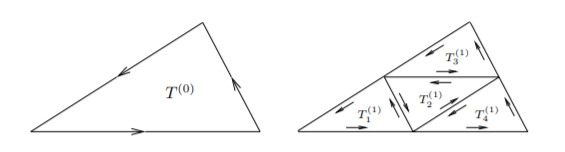
\includegraphics[height=8cm,width=16cm]{triangle.png} 
   \end{minipage}
\end{center}

Obviously, we may parametrize the boundaries of these triangles so that 
\begin{align*}
\int_{ \partial T^{(0)}}fdz= \sum_{n=1}^4 \int_{\partial T^{(1)}_n} fdz
\end{align*}
Taking absolute value on both side, we deduce 
\begin{align*}
  \abso{\int_{\partial  T^{(0)}}fdz }\leq 4 \abso{\int_{\partial  T^{(1)}_j}fdz}\text{ for some $j \in \set{1,2,3,4}$}
\end{align*}
Denote $T_j^{(1)}$ by $T^{(1)}$. Repeating this process, we obtain a decreasing sequence of triangles 
\begin{align*}
T^{(0)} \supseteq T^{(1)} \supseteq \cdots \supseteq T^{(n)} \supseteq \cdots 
\end{align*} 
with the property that
\begin{align}
\label{pe1}
\abso{\int_{\partial  T^{(0)}}fdz}\leq 4^n \abso{\int_{\partial T^{(n)}}fdz}
\end{align}
Let $d^{(n)}\text{ and }p^{(n)}$ denote the diameter and perimeter of $T^{(n)}$ for all $n\inz_0^+$. Some tedious effort shows that 
\begin{align}
\label{pe2}
d^{(n)}=2^{-n}d^{(0)}\text{ and }p^{(n)}=2^{-n}p^{(0)}
\end{align}
\myref{Theorem}{DSoC} implies 
\begin{align*}
\bigcap_{n\inn} T^{(n)}=\set{z_0}\text{ for some }z_0 \in D
\end{align*}
Because $f$ is holomorphic at  $z_0$, we may write $f:D\rightarrow \C$ by 
\begin{align*}
f(z)=f(z_0)+f'(z_0)(z-z_0)+o(z-z_0)(z-z_0)
\end{align*}
Clearly the first two terms have antiderivatives. Using \myref{Equation}{pe1} and \myref{Equation}{pe2}, we may now estimate 
\begin{align*}
 \abso{\int_{\partial T^{(0)}}f(z)dz}\leq  4^n\abso{\int_{\partial T^{(n)}} f(z)dz}&= 4^n\abso{\int_{\partial  T^{(n)}} o(z-z_0)(z-z_0)dz}\\
  &\leq 4^np^{(n)}d^{(n)}\max_{ z\in \partial T^{(n)}}\abso{o(z-z_0)}\\
  &= p^{(0)}d^{(0)} \max_{z \in \partial T^{(n)}} \abso{o(z-z_0)}\to 0\text{ as }n\to \infty
\end{align*}
\end{proof}
\begin{mdframed}
By $D\subseteq \C$ being \textbf{star-convex with center $z_*$}, we mean that for all $z \in D$, the contour $\gamma :[0,1]\rightarrow \C$ defined by 
\begin{align*}
\gamma (t)\triangleq z_*+t(z-z_*)
\end{align*}
satisfy $\gamma ([0,1])\subseteq D$. 
\end{mdframed}
\begin{theorem}
\textbf{(Existence of antiderivative on star-convex domain)} Suppose $D\subseteq \C$ is open and star-convex with centre  $z_*$. If $f:D\rightarrow \C$ is holomorphic, then $F:D\rightarrow \C$ defined by 
\begin{align*}
F(z)\triangleq \int_\gamma f(w)dw\text{ where }\gamma :[0,1]\rightarrow D\text{ is defined by }\gamma(t)\triangleq z_*+t(z-z_*)
\end{align*}
is an antiderivative of $f$. 
\end{theorem}
\begin{proof}
Fix $z_0 \in D$. Because $D$ is open, there exists some open ball $B_\epsilon (z_0)$ small enough to be contained by $D$. For all $z\in B_\epsilon (z_0)$, the closed triangle $T$ specified by the vertices $\set{z_*,z,z_0}$ is contained by $D$, since all $p\in  T$ lies in some line segment joining $z_*$ and $w$ where $w$ is some point that lies in the line segment joining $z$ and  $z_0$.  We then can apply \customref{CTft}{Cauchy's Integral Theorem for triangles} to have the estimate 
\begin{align*}
  \abso{\frac{F(z)-F(z_0)}{z-z_0}-f(z_0)}&= \abso{\frac{\int_\gamma [f(w)-f(z_0)]dw}{z-z_0}}\\
  &\leq \max_{w \in \gamma }\abso{f(w)-f(z_0)}\to 0\text{ as }z \to z_0
\end{align*}
where $\gamma$ is the line segment traveling from $z_0$ to  $z$.  
\end{proof}
\begin{mdframed}
At this point, it is appropriate for us to define \textbf{the winding number $w(\gamma ,z_0)$ of a contour $\gamma :[a,b]\rightarrow \C$ around some point $z_0\not\in \gamma $} by 
\begin{align*}
w(\gamma ,z_0)\triangleq  \frac{1}{2\pi  i}\int_{\gamma } \frac{1}{z-z_0}dz
\end{align*}
Immediately, we see that our definition satisfy our geometric intuition in the sense that the circle $\gamma :[0,2\pi  ]\rightarrow \C$ is defined by 
\begin{align*}
\gamma (t)\triangleq z_0 + e^{it}
\end{align*}
have winding number  
\begin{align*}
w(\gamma ,z_0)= \frac{1}{2\pi i}\int_0^{2\pi } e^{- it }ie^{it}dt= 1
\end{align*}
Moreover, we expect any closed contour $\gamma :[a,b]\rightarrow \C$ to have integer-valued winding number. This is true. Consider $f:[a,b]\rightarrow \C$ defined by 
\begin{align*}
f(t)\triangleq \frac{1}{2\pi  i}\int_a^t \frac{\gamma '(s)}{\gamma (s)-z_0}ds
\end{align*}
One may check by direct computation that 
\begin{align*}
\frac{d}{dt}e^{-2\pi  if (t)}(\gamma (t)-z_0)\equiv 0 
\end{align*}
It then follows from $\gamma $ being closed that 
\begin{align*}
e^{-2\pi  if(a)}=e^{-2\pi  if(b)}
\end{align*}
which implies 
\begin{align*}
w(\gamma ,z_0)=f(b)=f(a)+n=n\inz
\end{align*}
Given some contour $\gamma :[a,b]\rightarrow \C$, if we define $g:\C\setminus \gamma \rightarrow \C$ by 
\begin{align*}
g(z)\triangleq w(\gamma ,z)
\end{align*}
we see that $g$ is continuous, since if $z_0\not\in \gamma $, we may find $D_r(z_0)$ disjoint with $\gamma $ and obtain the estimate 
 \begin{align*}
\abso{w(\gamma ,z_0)-w(\gamma ,z_1)}&= \frac{1}{2\pi  }\abso{\int_\gamma \Big[ \frac{1}{z-z_0}-\frac{1}{z-z_1} \Big]dz} \\
&=\frac{1}{2\pi  }\abso{\int_{\gamma } \frac{z_1-z_0}{(z-z_0)(z-z_1)}dz} \\
&\leq \frac{L \abso{z_1-z_0}}{ r^2 \pi  }\text{ where }L\text{ is the length of }\gamma 
\end{align*}
as long as $\abso{z_0-z_1}<\frac{r}{2}$. The continuity of $g$ together with the fact that  $g$ can only be integer-valued implies that  $g$ is constant on any connected component of  $\C \setminus \gamma $. We may now finally state our version of \customref{CIT}{Cauchy Integral Theorem}. 
\end{mdframed}
\begin{theorem}
\label{CIT}
\textbf{(Cauchy Integral Theorem)} Suppose $D\subseteq \C$ is open and $f:D\rightarrow \C$ is holomorphic. If $\gamma :[a,b]\rightarrow \C$ is a closed contour lying in $D$ such that  $w(\gamma ,z)=0$ for all $z\not\in D$, then 
\begin{align*}
\int_\gamma  fdz=0 
\end{align*}
\end{theorem}
\begin{proof}
As Prof Frank remarked, the proof is omitted here for being too long and tricky. 
\end{proof}
\begin{theorem}
\label{CIF}
\textbf{(Cauchy Integral Formula)}  Let $U\subseteq \C$ be open, $D$ be an closed disk contained by  $U$, and $C$ be a closed contour running through the boundary of $D$ counterclockwise. If $f:U\rightarrow \C$ is holomorphic and $a\in D^\circ $, then 
\begin{align*}
f(a)= \frac{1}{2\pi  i}\int_C \frac{f(z)}{z-a}dz
\end{align*}
\end{theorem}
\begin{proof}
Fix $\epsilon $. Let $\delta$ satisfy 
\begin{align*}
\abso{z-a}\leq \delta \implies  \abso{f(z)-f(a)}\leq \epsilon 
\end{align*}
With a geometric argument using \customref{CIT}{Cauchy Integral Theorem}, one have 
\begin{align*}
\int_C \frac{f(z)}{z-a}dz=  \int_{\gamma  } \frac{f(z)}{z-a}dz
\end{align*}
where $\gamma :[0,2\pi ]\rightarrow D^\circ $ is defined by  
\begin{align*}
\gamma (t)\triangleq a+ \delta e^{it} 
\end{align*}
The proof then follows from the estimation 
\begin{align*}
  \abso{f(a)- \frac{1}{2\pi i}  \int_C \frac{f(z)}{z-a}dz}&= \abso{f(a)- \frac{1}{2\pi  i}\int_\gamma  \frac{f(z)}{z-a}dz} \\
                              &= \abso{f(a)- \frac{1}{2\pi  i}\int_0^{2\pi  } \frac{f(a+ \delta e^{it})}{\delta e^{it} } i\delta e^{i t} dt}  \\
                              &= \frac{1}{2\pi } \abso{\int_0^{2\pi  } f(a+ \delta e ^{it})- f(a)dt}\leq \epsilon 
\end{align*}
\end{proof}
\begin{theorem}
\label{Hfaa}
\textbf{(Holomorphic functions are analytic)} Let $U\subseteq \C$ be an open, $D$ be an closed disk contained by $U$ and centering $a$ with radius  $R$. Let $C$ be a closed contour running through the boundary of $D$ counterclockwise. If we define for all $n\geq 0$ 
\begin{align*}
c_n\triangleq  \frac{1}{2 \pi  i}\int_C \frac{f(z)}{(z-a)^{n+1}}dz
\end{align*}
then the power series 
\begin{align*}
  \sum_{n=0}^{\infty} c_n (z-a)^n
\end{align*}
agrees with $f$ on $D^{\circ }$. 
\end{theorem}
\begin{proof}
Let $z\in D^{\circ }$. By \customref{CIF}{Cauchy's Integral Formula}, we have 
\begin{align*}
f(z)&= \frac{1}{2\pi  i}\int_C \frac{f(w)}{w-z}dw \\
&=\frac{1}{2\pi  i}\int_C f(w)\Big[ \frac{1}{w-a} + \frac{z-a}{(w-a)^2}+ \cdots + \frac{(z-a)^m}{(w-a)^{m+1}} + \frac{(z-a)^{m+1}}{(w-a)^{m+1}(w-z)} \Big]dw \\
&=\sum_{n=0}^{m} c_n (z-a)^n + \frac{1}{2\pi  i}\int_C \frac{(z-a)^{m+1}}{(w-a)^{m+1}(w-z)}dw
\end{align*}
The proof then follows from noting  $\abso{\frac{z-a}{w-a}}<1$ and direct estimation of \myref{Equation}{LM}. 
\end{proof}
\begin{mdframed}
What follows from the fact  \customref{Hfaa}{holomorphic functions are analytic} and 
\customref{TT}{Taylor's Theorem for Power Series} is that if $f$ is holomorphic on some open disk  $D_{r+\epsilon }(a)$ and $C$ is the closed contour running through the boundary of  $D_r(a)$ counterclockwise, then we have a nice formula  
\begin{align*}
f^{(n)}(a)=  \frac{n!}{2\pi  i}\int_C \frac{f(z)}{(z-a)^{n+1}}dz
\end{align*}
which agrees with our \customref{CIF}{Cauchy integral Formula}.\\ 

In particular, we often encounter  complex function $f:\C\rightarrow \C$ that is \textbf{entire}, i.e., $f$ is holomorphic on the whole $\C$. \myref{Theorem}{Hfaa} states that for all $R>0$, if we let  $C$ be the closed contour running through the boundary of the open disk centering $0$ with radius  $R$  counterclockwise, then 
\begin{align*}
f=\sum_{n=0}^{\infty}c_{n,R} z^n \text{ on the open disk with radius }R
\end{align*}
for $c_{n,R}$ given in \myref{Theorem}{Hfaa}. Let $R_1< R_2$. Trivially, 
\begin{align*}
\sum_{n=0}^{\infty} c_{n,R_1}z^n=\sum_{n=0}^{\infty} c_{n,R_2}z^n\text{ on the open disk with radius }R_1
\end{align*}
It then follows from \customref{Identity Theorem}{Identity Theorem} that 
\begin{align*}
c_{n,R_1}=c_{n,R_2}\text{ for all }n
\end{align*}
Letting $R\to \infty$, we may now just write 
\begin{align*}
f(z)= \sum_{n=0}^{\infty}c_nz^n\text{ on }\C
\end{align*}
\end{mdframed}
\begin{theorem}
\label{LV}
\textbf{(Liouville's Theorem)} If entire $f:\C\rightarrow \C$ is bounded, then $f$ is constant. 
\end{theorem}
\begin{proof}
Write 
\begin{align*}
f(z)=\sum_{n=0}^{\infty}c_nz^n\text{ on }\C
\end{align*}
By \myref{Theorem}{Hfaa}, 
\begin{align*}
c_n= \frac{1}{2\pi i}\int_{C_r} \frac{f(z)}{z^{n+1}}dz
\end{align*}
where $C_r$ is the closed contour running through the boundary of the open disk centering  the origin with radius  $r$. Let $n\geq 1$, and let  $M$ be an upper bound of $\abso{f}$. The proof then following from letting $r \to \infty$ in the below estimation 
\begin{align*}
\abso{c_n}= \frac{1}{2\pi } \cdot (2\pi r) \cdot \max_{C_r} \abso{\frac{f(z)}{z^{n+1}}} \leq \frac{M}{r^n}
\end{align*}
\end{proof}
\section{Residue Formula}
\begin{abstract}

\end{abstract}
\begin{mdframed}
Before we begin developing this section, we first give the following remark. Let  
\begin{align*}
0<R_1 <r_1<r_2<R_2 < \infty
\end{align*}
Let $C_1,C_2$ respectively be closed contours running through the boundary of $D_{r_1}(0),D_{r_2}(0)$. If $f$ is holomorphic on on $R_1 < \abso{z}<R_2$, then 
\begin{align*}
\int_{C_1} f(z)dz= \int_{C_2}f(z)dz
\end{align*}
by a simple geometric argument. Therefore, we may give the next Theorem a well-defined statement. 
\end{mdframed}
\begin{theorem}
\label{LTC}
\textbf{(Laurent's Theorem)} Suppose
\begin{align*}
0\leq R_1 <r< R_2 \leq \infty
\end{align*}
$C_r$ is a closed contour running through the circle centering $z_0$ with radius $r$ counterclockwise, and $f$ is holomorphic on the annulus $R_1 < \abso{z-z_0} < R_2$. If we define 
\begin{align*}
c_n\triangleq  \frac{1}{2\pi  i} \int_{C_r} \frac{f(z)}{(z-z_0)^{n+1}}dz\text{ for all }n\inz
\end{align*}
Then $\sum_{n\geq 0} c_nh^n$ converge for $\abso{h}<R_2$, $\sum_{n<0} c_nh^{n}$ converge for $\abso{h}>R_1$ and 
\begin{align*}
f(z_0+h)= \sum_{n\inz} c_nh^n\text{ on the annulus }R_1 < \abso{h}< R_2
\end{align*}
\end{theorem}
\begin{proof}
Fix some  $h\inc$ such that $R_1 < \abso{h}<R_2$. Let $r_1,r_2$ satisfy 
 \begin{align*}
R_1 < r_1 < \abso{h}< r_2 < R_2
\end{align*}
And let $C_{r_1},C_{r_2}$ respectively be closed contours running through the circle centering $z_0$ with radius  $r_1,r_2$ counterclockwise. We first show that 
\begin{align*}
  \vi{f(z_0+h)= \frac{1}{2\pi  i}\int_{C_{r_1}} \frac{f(z)}{z-(z_0+h)}dz- \frac{1}{2\pi i}\int _{C_{r_2}} \frac{f(z)}{z-(z_0+h)}dz}
\end{align*}
\end{proof}
\begin{mdframed}
With \customref{LTC}{Laurent's Theorem}, given holomorphic $f:D_\epsilon (z_0)\setminus \set{z_0}\rightarrow \C$, we may write 
\begin{align*}
f(z)= \sum_{n\inz} c_n (z-z_0)^n\text{ for } 0<\abso{z-z_0}< \epsilon 
\end{align*}
If $c_n=0$ for all $n<0$, obviously we may define  $f(z_0)\triangleq c_0$, so that $f$ is still holomorphic after such extension. If this is the case, we say $f$ has a  \textbf{removable singularity at $z_0$}.     
\end{mdframed}
\begin{theorem}
\label{RoRS}
\textbf{(Riemann's removable singularity Theorem)} Given holomorphic $f:D_\epsilon (z_0)\setminus \set{z_0}\rightarrow \C$ 
\begin{align*}
z_0\text{ is a removable singularity of $f$ }\iff f\text{ is bounded on some }D_\delta (z_0)\setminus \set{z_0}
\end{align*}
\end{theorem}
\begin{proof}
From left to right is clear. Suppose $f$ is bounded by $M$ on $D_\delta(z_0)\setminus \set{z_0}$. Because 
\begin{align*}
c_n=\frac{1}{2\pi  i}\int_{C_r}f(z)(z-z_0)^{-n-1}dz
\end{align*}
We may estimate 
\begin{align*}
  \abso{c_n}\leq \frac{1}{2\pi }(2\pi r )( M r^{-n-1})= Mr^{-n}
\end{align*}
The proof then follows from letting $n<0$ and $r \to 0$. 
\end{proof}
\begin{mdframed}
If for some $m<0$, we have  
 \begin{align*}
c_m \neq 0\text{ and }c_n=0\text{ for all }n\leq m
\end{align*}
then we say $f$ has a  \textbf{pole of order $m$ at  $z_0$}. If a pole is of order $1$, we say such pole is a  \textbf{simple pole}.  
\end{mdframed}
\begin{theorem}
\textbf{(Recognition of Pole)} Given holomorphic $f:D_\epsilon (z_0)\setminus \set{z_0}\rightarrow \C$ 
\begin{align*}
f\text{ has a pole of order }m\text{ at }z_0\iff \lim_{z\to z_0}(z-z_0)^mf(z)\inc^*
\end{align*}
\end{theorem}
\begin{proof}
From left to right is clear. From right to left, define $g:D_\epsilon (z_0)\setminus \set{z_0}\rightarrow \C$ by 
\begin{align*}
g(z)\triangleq (z-z_0)^m f(z)
\end{align*}
From premise, we may deduce $g$ is bounded on some  $D_\delta(z_0)\setminus \set{z_0}$. Therefore, by \myref{Theorem}{RoRS}, $g$ has a removable singularity at $z_0$. Thus, we may write 
 \begin{align*}
g(z)=\sum_{n=0}^{\infty}a_n z^n
\end{align*}
where $a_0\neq 0$ by premise. The proof then follows from writing $f$ in terms of $a_n$.  
\end{proof}
\begin{mdframed}
Writing holomorphic $f:D_\epsilon (z_0)\setminus \set{z_0}\rightarrow \C$ in terms of Laurent Series  
\begin{align*}
f(z)= \sum_{n\inz} c_n (z-z_0)^n 
\end{align*}
We define the \textbf{residue of $f$ at  $z_0$} to be 
\begin{align*}
\operatorname{Res}(f,z_0)\triangleq c_{-1}
\end{align*}
If there are infinitely many $n<0$ such that $c_n\neq 0$, we say $f$ has a \textbf{essential singularity} at $z_0$. Obviously, if  $f$ has a removable singularity at  $z_0$, then the residue of  $f$ at $z_0$ is  $0$. Immediately, from direct computation with Laurent expansion of $f:D_\epsilon (z_0)\setminus \set{z_0}\rightarrow \C$, we may conclude the following easy ways to compute residue for relatively simple function. 
\end{mdframed}
\begin{theorem}
\textbf{(Calculation of Residue)} If holomorphic $p,q:D_\epsilon (z_0)\rightarrow \C$ satisfies 
\begin{align*}
p(z_0)\neq 0\text{ and }q(z_0)=0,q'(z_0)\neq 0 
\end{align*}
Then $f=\frac{p}{q}$ has a simple pole at $z_0$ and 
 \begin{align*}
\operatorname{Res}(f,z_0)= \frac{p(z_0)}{q'(z_0)}
\end{align*}
If $f:D_\epsilon (z_0)\setminus \set{z_0}\rightarrow \C$ has a pole of order $m$ at  $z_0$,  then 
 \begin{align*}
\operatorname{Res}(f,z_0)=  \lim_{z\to z_0} \frac{1}{(m-1)!} \Big( \frac{d}{dz} \Big)^{m-1} (z-z_0)^m f(z)
\end{align*}
\end{theorem}
\begin{theorem}
\label{CRT}
\textbf{(Cauchy's Residue Theorem)} Suppose that $f$ is holomorphic in an open set containing a positively oriented  Jordan curve $\gamma $ and its interior, except for poles at the points $z_1,\dots ,z_N$ inside $\gamma $. Then 
\begin{align*}
\int_{\gamma }f(z)dz = 2\pi  i\sum_{n=1}^N \operatorname{Res} (f,z_n)
\end{align*}
\end{theorem}
\begin{mdframed}
  Using \customref{CRT}{the residue theorem}, we may compute the following integral that will definitely exists in context of Fourier analysis.   
\end{mdframed}
\begin{Example}{\textbf{(Poisson Kernel)}}{}
\begin{align*}
  \int_0^{\pi } \frac{\log x}{1+x^2}dx
\end{align*}
\end{Example}
\begin{mdframed}
Let $D \subseteq \C$ be open connected, $f:D\rightarrow \C$ be holomorphic. Suppose $f$ does not vanish identically on  $D$.  \customref{Identity Theorem}{Identity Theorem} tell us that the set of \textbf{zeros}
\begin{align*}
Z\triangleq \set{z\in D: f(z)=0}
\end{align*}
must have no limit point in $D$. Therefore, for each zero $z_0 \in Z$, when we write locally 
\begin{align*}
  f(z)= \sum_{n=0}^{\infty} c_n(z-z_0)^n
\end{align*}
there exists some smallest $n\geq 1$ such that $c_n \neq 0$. We then say $f$ has a  \textbf{zero of order $n$ at $z_0$}, and if  $n=1$, we say this zero is  \textbf{simple}. \\

Let $z_0\inc$. Given some holomorphic $f:D_\epsilon (z_0)\setminus \set{z_0}\rightarrow \C$, we say $f$ has a \textbf{removable singularity at $z_0$} if we may define $f(z_0)$ to be some complex number so that $f:D_\epsilon (z_0)\rightarrow \C$ is holomorphic. Suppose $f:D_\epsilon (z_0)\setminus \set{z_0}\rightarrow \C^*$. We say $f$ has a  \textbf{pole of order $n$ at $z_0$} if the function $g:D_\epsilon (z_0)\rightarrow \C$ defined by 
\begin{align*}
g(z)\triangleq \begin{cases}
  \frac{1}{f(z)}& \text{ if $z\neq z_0$ }\\
  0& \text{ if $z=z_0$ }
\end{cases}
\end{align*}
is holomorphic with the order $n$ at zero  $z_0$. Obviously, there exists an unique holomorphic $h:D_\epsilon (z_0)\rightarrow \C$ such that 
\begin{align*}
g(z)= (z-z_0)^n h(z)
\end{align*}
It is clear that $h$ does not vanish on  $D_\epsilon (z_0)$. Therefore, we may write 
\begin{align*}
G(z)= \frac{1}{h(z)}
\end{align*}
so that $G:D_\epsilon (z_0)\rightarrow \C$ is holomorphic and write 
\begin{align*}
f(z)= \frac{G(z)}{(z-z_0)^n}=\sum_{k=-n}^{\infty}a_k (z-z_0)^k
\end{align*}
We then call 
\begin{align*}
\sum_{k=-n}^{-1}a_k(z-z_0)^k
\end{align*}
the \textbf{principal part of $f$ at the pole $z_0$} and 
\begin{align*}
\operatorname{Res}_{z_0}f\triangleq a_{-1}
\end{align*}
the \textbf{residue of $f$ at the pole  $z_0$}. It is clear from the Laurent expansion of $f$ and direct computation that   
\begin{align*}
\operatorname{Res}_{z_0}f=
\end{align*}
\end{mdframed}
\section{Script}
\begin{question}{}{}
There are three types of isolated singularities: removable singularity, poles and essential singularity. Provide the definition of each type and give an example.  
\end{question}
\begin{proof}
Let $f:D_\epsilon (z_0)\setminus \set{z_0}\rightarrow \C$ be holomorphic so that $f$ has an isolated singularity at  $z_0$. By Laurent's Theorem, we may express $f$ as a Laurent series 
\begin{align*}
f(z)= \sum_{n=-\infty}^{\infty} c_n(z-z_0)^n
\end{align*}
If $c_n=0$ for all negative $n$, say 
\begin{align*}
f(z)= (z-z_0)^2 + 7 \text{ on }D_\epsilon (z_0)\setminus \set{z_0}
\end{align*}
we say $f$ has a removable singularity at $z_0$. If there are only finite numbers of negative $n$ such that $c_n\neq 0$, and $m$ is the smallest integer such that
\begin{align*}
c_n \neq 0 \text{ for }n=m
\end{align*}
we say $f$ has a pole of order $m$ at $z_0$. For example, $f$ can be 
 \begin{align*}
f(z)=\frac{1}{z-z_0}\text{ on }D_\epsilon (z_0)\setminus \set{z_0}
\end{align*}
If there are infinite number of negative $n$ such that  $c_n \neq 0$, for example, 
\begin{align*}
f(z)= e^{\frac{1}{(z-z_0)}}= \sum_{n=0}^{\infty} \frac{1}{n!}(z-z_0)^{-n}\text{ on }D_\epsilon (z_0)\setminus \set{z_0}
\end{align*}
we say $f$ has an essential singularity at $z_0$. 
\end{proof}
\begin{question}{}{}
State the definition of the residue of a function at an isolated singularity. 
\end{question}
\begin{proof}
Let $f:D_\epsilon (z_0)\setminus \set{z_0}\rightarrow \C$ be holomorphic so that $f$ has an isolated singularity at  $z_0$. By Laurent's Theorem, we may express $f$ as a Laurent series 
\begin{align*}
f(z)= \sum_{n=-\infty}^{\infty} c_n(z-z_0)^n
\end{align*}
The residue of $f$ at  $z_0$ is defined to be $c_{-1}$. 
\begin{align*}
\operatorname{Res}(f,z_0)\triangleq c_{-1}
\end{align*}
\end{proof}
\begin{question}{}{}
If $z_0$ is a simple pole of  $f$, prove that 
\begin{align*}
\operatorname{Res}(f,z_0)= \lim_{z\to z_0} (z-z_0)f(z)
\end{align*}
\end{question}
\begin{proof}
Because $z_0$ is a simple pole of  $f$, we may write 
 \begin{align*}
   f(z)= [\operatorname{Res}(f,z_0)](z-z_0)^{-1}+ \sum_{n=0}^{\infty} c_n(z-z_0)^n
\end{align*}
This give us 
\begin{align*}
\lim_{z\to z_0}(z-z_0)f(z)&= \lim_{z\to z_0}\operatorname{Res}(f,z_0)+ \sum_{n=0}^{\infty}c_n(z-z_0)^{n+1} \\
&=\operatorname{Res}(f,z_0)+ \sum_{n=0}^{\infty} \lim_{z\to z_0}c_n (z-z_0)^{n+1} \\
&=\operatorname{Res}(f,z_0)
\end{align*}
\end{proof}
\begin{question}{}{}
If  $f(z)=\frac{q(z)}{p(z)}$ where $p$ and $q$ are holomorphic, and  $z_0$ is a simple zero of  $p$, prove that 
\begin{align*}
\operatorname{Res}(f,z_0)= \frac{q(z_0)}{p'(z_0)}
\end{align*}
\end{question}
\begin{proof}
Because $z_0$ is a simple zero of $p$, we know 
\begin{align*}
p'(z_0)\neq 0
\end{align*}
If $q(z_0)\neq 0$, then $f$ has a simple pole at $z_0$, and from result of last question we may compute 
 \begin{align*}
\operatorname{Res}(f,z_0)&= \lim_{z\to z_0} \frac{(z-z_0)q(z)}{p(z)-p(z_0)}= \frac{q(z_0)}{p'(z_0)} 
\end{align*}
\end{proof}
\begin{question}{}{}
If $z_0$ is a pole of  $f$ of order $m$, prove that 
 \begin{align*}
\operatorname{Res}(f,z_0)=\lim_{z\to z_0} \frac{1}{(m-1)!}\Big(\frac{d}{dz}\Big)^{m-1} g(z)
\end{align*}
where $g(z)=(z-z_0)^m f(z)$
\end{question}
\begin{proof}
Because $z_0$ is a pole of $f$ of order $m$, we may write 
 \begin{align*}
f(z)=\sum_{n=-m}^\infty c_n (z-z_0)^n\text{ and }g(z)=\sum_{n=0}^{\infty} c_{n-m}(z-z_0)^n
\end{align*}
Or write 
\begin{align*}
  g(z)= c_{-m}+c_{-m+1} (z-z_0)   + \cdots + c_{-1}(z-z_0)^{m-1} + c_0(z-z_0)^m +\cdots 
\end{align*}
Compute 
\begin{align*}
g^{(m-1)}(z)= \frac{(m-1)!}{0!}c_{-1}+\frac{m!}{1!}c_0(z-z_0)+ \frac{(m+1)!}{2!}c_1(z-z_0)^2 + \cdots  
\end{align*}
This give us 
\begin{align*}
\lim_{z\to z_0} \frac{1}{(m-1)!}g^{(m-1)}(z)= c_{-1}= \operatorname{Res}(f,z_0)
\end{align*}
\end{proof}
\begin{question}{}{}
Find the residue of the following function at the indicated points: 
\begin{enumerate}[label=(\alph*)]
  \item $\frac{z}{(2-3z)(4z+3)}$ at $z= \frac{2}{3}$. 
  \item $\frac{z-\frac{1}{6}z^3 - \sin z}{z^8}$ at $z=0$. 
\end{enumerate}
\end{question}
\begin{proof}
For the first function, observe  
\begin{align*}
\lim_{z\to \frac{2}{3}} (z- \frac{2}{3}) \cdot \frac{z}{(2-3z)(4z+3)}= \lim_{z\to \frac{2}{3}}\frac{z}{-3(4z+3)}= \frac{2}{-51}\neq 0
\end{align*}
which implies $z=\frac{2}{3}$ is a simple pole. Therefore, from the question earlier, we may deduce its residue is exactly $\frac{2}{-51}$. For the second function, we can just compute its Laurent series by 
\begin{align*}
\frac{z- \frac{1}{6}z^3- \sin z}{z^8}&= \frac{1}{z^7}- \frac{1}{6z^5} - \frac{1}{z^8}\sum_{n=0}^{\infty}  \frac{(-1)^n}{(2n+1)!}z^{2n+1} \\
&=\frac{1}{5!}z^{-3}+ \frac{-1}{7!}z^{-1}+ \frac{1}{9!}z + \cdots 
\end{align*}
Therefore, its residue is $\frac{-1}{7!}$. 
\end{proof}
\begin{question}{}{}
Evaluate 
\begin{align*}
\int_{-\pi }^{\pi } \frac{d\theta}{5+ 3 \cos \theta}
\end{align*}
\end{question}
\begin{proof}
Define $\gamma :[-\pi ,\pi ]\rightarrow \C$ by 
\begin{align*}
\gamma (t)=e^{it}
\end{align*}
We have 
\begin{align*}
I\triangleq -2i\int _{\gamma } \frac{dz}{3z^2+10z+3}&= \int_\gamma  \frac{dz}{\frac{3i}{2}z^2 + 5iz+ \frac{3}{2}i} \\
&=\int_{\gamma } \frac{1}{5+ \frac{3}{2}(z+ \frac{1}{z})} \cdot \frac{1}{iz} dz\\
&=\int_{-\pi }^{\pi } \frac{1}{5+ \frac{3}{2}(e^{it}+e^{-it})} \cdot \frac{ie^{ it}}{i e^{it}}dt \\
&=\int_{-\pi }^{\pi } \frac{1}{5+ 3 \cos t}dt
\end{align*}
In summary 
\begin{align*}
\int_{-\pi }^{\pi } \frac{d\theta}{5+ 3 \cos \theta}&= -2i \int_{\gamma } \frac{dz}{3z^2+10z+3} 
\end{align*}
Note that 
\begin{align*}
\frac{1}{3z^2+10+3}= \frac{1}{(3z+1)(z+3)}
\end{align*}
have two simple poles $z=-3$ and  $z= \frac{1}{-3}$, and have residue $\frac{1}{8}$ at pole $z=\frac{1}{-3}$. It then follows from residue theorem that 
\begin{align*}
\int_{-\pi }^{\pi } \frac{d\theta}{5+ 3 \cos \theta}= - 2i \cdot 2\pi  i \cdot \frac{1}{8}= \frac{\pi }{2} 
\end{align*}
\end{proof}
\begin{question}{}{}
Evaluate 
\begin{align*}
\int^{\infty}_{- \infty } \frac{dx}{x^2+2x+2}
\end{align*}
\end{question}
\begin{proof}
Let $S_R:[0 ,\pi ]\rightarrow \C$ be the semi-circle $S_R(t)\triangleq Re^{it}$, $L_R:[-R,R]\rightarrow \C$ be the line segment $L_R(t)\triangleq t$, and $\gamma$ the wedge $\gamma =S_R+L_R$. By residue theorem, 
\begin{align*}
\int_{\gamma } \frac{dz}{z^2+2z+2}= 2\pi i \cdot \frac{1}{2i}=\pi 
\end{align*}
for large enough $R$. Observe 
\begin{align*}
  \abso{\int_{S_R} \frac{dz}{z^2+2z+2} }\leq \pi R \cdot \max_{S_R} \frac{1}{\abso{z+1-i}\cdot \abso{z+1+i}} \leq  \frac{\pi  R}{(R- \sqrt{2} )^2} 
\end{align*}
This implies 
\begin{align*}
\lim_{R\to \infty} \int_{S_R} \frac{dz}{z^2+2z+2}= 0
\end{align*}
Therefore, 
\begin{align*}
\int_{-\infty}^{\infty} \frac{dx}{x^2+2x+2}&= \lim_{R\to \infty}\int_{L_R} \frac{dz}{z^2+2z+2} \\
&=\lim_{R\to \infty} \pi  - \int_{S_R} \frac{dz}{z^2+2z+2}=\pi 
\end{align*}
\end{proof}
\begin{question}{}{}
Evaluate 
\begin{align*}
\int_{-\infty}^{\infty} \frac{dx}{x^4+2x^2+1}
\end{align*}
\end{question}
\begin{proof}
Let $S_R:[0 ,\pi ]\rightarrow \C$ be the semi-circle $S_R(t)\triangleq Re^{it}$, $L_R:[-R,R]\rightarrow \C$ be the line segment $L_R(t)\triangleq t$, and $\gamma$ the wedge $\gamma =S_R+L_R$. By residue theorem, 
\begin{align*}
\int_{\gamma } \frac{dz}{z^4+2z^2+1}= 2\pi  i \lim_{z\to i} \frac{d}{dz} \frac{1}{(z+i)^2}= \frac{\pi }{2}
\end{align*}
for large enough $R$. Observe 
 \begin{align*}
\abso{\int_{S_R} \frac{dz}{z^4+2z^2+1}}\leq \pi  R \cdot \max_{S_R} \frac{1}{\abso{z+i}^2 \cdot \abso{z-i}^2}\leq \frac{\pi  R}{(R-1)^4}
\end{align*}
This implies 
\begin{align*}
\lim_{R\to \infty} \int_{S_R} \frac{dz}{z^4+2z^2+1} = 0
\end{align*}
Therefore, 
\begin{align*}
\int_{-\infty}^{\infty} \frac{dx}{x^4+ 2x^2+1}&= \lim_{R\to \infty} \int_{L_R} \frac{dz}{z^4+2z^2+1} \\
&=\lim_{R\to \infty} \frac{\pi }{2}- \int_{S_R} \frac{dz}{z^4+2z^2+1}= \frac{\pi }{2}
\end{align*}
\end{proof}
\section{Dirichlet's Problem}
\begin{mdframed}
Let $D(R)\subseteq \R^2$ denote the unit open disk, and let $g:\partial D(R) \rightarrow \R$ be a  continuous function defined on the boundary. Dirichlet's problem asked: 
\begin{center}
   \begin{minipage}{0.9\linewidth}  
Is there continuous $u: \overline{D(R)}\rightarrow \R$ such that $u$ is harmonic on the interior and agree with $g$ on boundary? 
   \end{minipage}
\end{center}
Let's first suppose such $u$ exists. If we define $f:D(R)\rightarrow \C$ by 
\begin{align*}
f= \frac{\partial u}{\partial x}- i \frac{\partial u}{\partial y}
\end{align*}
then $f$ is holomorphic according to Cauchy-Riemann Theorem. Because $f$ is holomorphic, we may let $F:D(R)\rightarrow \C$ be its anti-derivative. It is clear that by computation that $F$ has the form
\begin{align*}
F= u+iv +C
\end{align*}
where $C$ is some constant. Let $C=0$. By \customref{CIF}{Cauchy Integral Formula}, for all $r<R$, we have 
 \begin{align*}
F(z)= \sum_{n=0}^{\infty} c_n z^n \text{ for }\abso{z}<r
\end{align*}
for some $c_n$. By \customref{Identity Theorem}{Identity Theorem}, we can just write 
\begin{align*}
F(z)=\sum_{n=0}^{\infty} c_nz^n \text{ for }\abso{z}<R
\end{align*}
If we write 
 \begin{align*}
c_n = \alpha _n + i \beta _n 
\end{align*}
because $u=\operatorname{Re}F$, we may compute 
\begin{align*}
u= \sum_{n=0}^{\infty} r^n (a_n \cos (n\theta)+b_n \sin (n \theta))\text{ on }D(R)
\end{align*}
where $a_n=\alpha_n$ and $b_n=-\beta_n$. Because $u$ is continuous, we know 
 \begin{align}
\label{lk}
g(\theta)=\lim_{r\to 1} \Big(\sum_{n=0}^{\infty}r^n (a_n \cos (n \theta)+ b_n \sin (n\theta)) \Big)\text{ exists }
\end{align}
It then follows from a non-trivial estimation (you may do this by yourself) that 
\begin{align*}
g(\theta)= \sum_{n=0}^{\infty} a_n \cos (n \theta)+ b_n \sin (n \theta)
\end{align*}
Because $g$ is continuous, we know 
\begin{align*}
a_n= \frac{1}{\pi }\int_{-\pi }^{\pi } g(\theta)\cos (n \theta) d\theta \text{ and }b_n = \frac{1}{\pi }\int_{-\pi }^{\pi }g(\theta)\sin (n \theta)d \theta \text{ for }n\geq 1
\end{align*}
and 
\begin{align*}
a_0= \frac{1}{2\pi }\int_{-\pi }^{\pi }g(\theta) d\theta
\end{align*}
We thus may write 
\begin{align}
\label{lk2}
u&=\sum_{n=0}^{\infty} r^n (a_n \cos (n\theta)+b_n \sin (n \theta))\text{ on }D(R)\\
&=  \frac{1}{2\pi }\int_{-\pi }^{\pi }g(\phi)d\phi +\sum_{n=1}^{\infty} \frac{r^n}{\pi } \int_{-\pi }^{\pi } g(\phi) \cos (n\phi)\cos (n \theta) + g(\phi) \sin (n \phi)\sin (n \theta)d \phi \notag  \\
&= \frac{1}{2\pi }\int_{-\pi }^{\pi }g(\phi)d\phi + \sum_{n=1}^{\infty} \frac{r^n}{\pi }\int_{-\pi }^{\pi }g(\phi) \cos \big(n (\theta- \phi)\big)  d\phi\notag  \\
&=\int_{-\pi }^{\pi }g(\phi) \Big[\frac{1}{2 \pi  }+\sum_{n=1}^{\infty} \frac{r^n}{\pi }\cos \big( n (\theta- \phi) \big) \Big]d\phi \text{ on }D(R)\notag 
\end{align}
Note that the last equality holds since the series is dominated by some constant multiples of $g$.    In fact, we can simplify the expression using the next lemma. 
\end{mdframed}
\begin{lemma}
For $0\leq r<1$ and $\xi\inr$, 
\begin{align*}
\frac{1}{2}+\sum_{n=1}^{\infty} r^n \cos ( n \xi)=  \frac{1}{2}\cdot \frac{1-r^2}{1-2r \cos (\xi) + r^2}
\end{align*}
\end{lemma}
\begin{proof}
Let $w=re^{i n \xi}$. Compute $\abso{w}=\abso{r}<1$. Therefore, 
\begin{align*}
\frac{1}{2}+\sum_{n=1}^{\infty} r^n \cos ( n \xi) &=\frac{1}{2}+ \frac{1}{2}\Big(\sum_{n=1}^{\infty} w^n +\overline{w^n}  \Big) \\
&=\frac{1}{2}\Big( \sum_{n=0}^{\infty}w^n + \sum_{n=1}^{\infty} \overline{w^n} \Big) \\
&=\frac{1}{2}\Big( \frac{1}{1-w}+ \frac{\overline{w}}{1- \overline{w}} \Big)\\
&= \frac{1}{2}\cdot \frac{1- \abso{w}^2}{ \abso{1-w}^2}= \frac{1}{2} \cdot \frac{1-r^2}{1-2r \cos \theta + r^2}
\end{align*}
\end{proof}
\begin{mdframed}
In conclusion, 
\begin{align*}
u= \frac{1}{2\pi }\int_{-\pi }^{\pi } g(\phi) \frac{1-r^2}{1-2r \cos (\theta- \phi)+r^2}d \phi \text{ on }D(R)
\end{align*}
The fact that this expression have boundary limit $g$ follows from \myref{Equation}{lk} and \myref{Equation}{lk2}. 
\end{mdframed}

\section{Archived}
\begin{theorem}
\textbf{(Cauchy Integral Theorem)} Suppose $D\subseteq \C$ is open and $f:D\rightarrow \C$ is holomorphic. If $\gamma :[a,b]\rightarrow \C$ is a closed contour lying in $D$ such that  $w(\gamma ,z)=0$ for all $z\not\in D$, then 
\begin{align*}
\int_\gamma  fdz=0 
\end{align*}
\end{theorem}
\begin{proof} 
We first shows that $\gamma $ is \textbf{pavable} on $[a,b]$, i.e, 
\begin{center}
   \begin{minipage}{0.9\linewidth}  
     \olive{There exists some partition $\set{a=t_0< \cdots < t_N=b}$ such that each sub-contour $\gamma_n$ obtained by restricting $\gamma $ to $[t_{n-1},t_n]$ lies inside an open disc $D_n\subseteq D$}
   \end{minipage}
\end{center}
\As{$\gamma $ is not pavable on $[a,b]$}. Bisect $[a,b]$  to get two closed intervals intersecting at the midpoint. We know $\gamma $ is unpavable on one of these intervals, otherwise $\gamma $ is pavable on $[a,b]$. Call this interval $I_1$ and bisect $I_1$ to get two closed interval intersecting at the midpoint of $I_1$ again. Similarly, one of these interval is unpavable, which we call $I_2$. Repeating the process, we have a sequence 
\begin{align*}
[a,b] \supseteq I_1 \supseteq I_2 \supseteq I_3 \supseteq \cdots 
\end{align*}
of compact intervals each with diameter $(b-a)2^{-n}$. It then follows from \myref{Theorem}{DSoC} that there exists some $t \in [a,b]$ such that 
\begin{align*}
\bigcap_{n=1}^{\infty} I_n =\set{t}
\end{align*}
Let $D_\epsilon$ be an open disk centering $\gamma (t)$ contained by $D$. It is clear that $\gamma ^{-1}(D_\epsilon )\subseteq [a,b]$ is some open set containing $t$. It follows that  $\gamma ^{-1}(D_\epsilon )$ contain some $I_n$ for some large enough  $n$. This implies $\gamma $ is pavable on $I_n$.  \CaC $\odone$\\

Define $\sigma_n:[t_{n-1},t_n]\rightarrow D_n$ by 

\end{proof}
\chapter{Beauty}
\label{Beauty}
\section{Fundamental Theorem of Algebra}
\begin{theorem}
\textbf{(Fundamental Theorem of Algebra)} Every non-constant complex polynomial $p:\C\rightarrow \C$ has at least one root. 
\end{theorem}
\begin{proof}
\As{$p$ has no root}. Because $p$ has no root, we may define  $q:\C\rightarrow \C$ by $q\triangleq p^{-1}$. It follows from \customref{Product and Quotient Rule for Holomorphic Function}{Quotient Rule} that $q$ is also entire. If we write $p=a_nz^n+ \cdots + a_0$, we have 
\begin{align*}
\abso{a_nz^n+ \cdots +a_0}\geq \abso{a_nz^n}- \abso{a_{n-1}z^{n-1}+ \cdots + a_0}
\end{align*}
Therefore, we may find some $R>0$ such that 
\begin{align*}
\abso{p(z)}>1 \text{ for all }z\not\in  \overline{D_R(0)}
\end{align*}
It follows that 
\begin{align*}
\abso{q(z)}\leq 1\text{ on }\C \setminus \overline{D_R(0)}
\end{align*}
Because $\abso{q}$ is continuous on $\overline{D_R(0)}$, it now follows from EVT that $q$ is indeed bounded on $\C$. Therefore, by \customref{LV}{Liouville's Theorem}, $q=\frac{1}{p}$ is a constant, impossible. \CaC
\end{proof}

\section{Euler's Formula}
\begin{abstract}
This section give a precise definition to exponential function and trigonometric functions, prove \customref{Euler's Formula}{Euler's Formula} and prove some of their basic properties seen in the real case. In this section, $z,v$ are complex numbers, and $x,y$ are real numbers.   
\end{abstract}
\begin{mdframed}
Suppose that we define 
\begin{align*}
\exp(z)&\triangleq \sum_{n=0}^\infty \frac{z^n}{n!}\\
\sin (z)&\triangleq \sum_{n=0}^\infty \frac{(-1)^n}{(2n+1)!}z^{2n+1}\\
\cos (z)&\triangleq \sum_{n=0}^\infty \frac{(-1)^n}{(2n)!}z^{2n}
\end{align*}
Some properties we are familiar with is now easily seen using \customref{Basic Technique on Sequence and Series}{basic techniques on sequence and series}. 
\begin{enumerate}[label=(\alph*)]
  \item Because \customref{Root Test is Stronger Than Ratio Test}{$\limsup_{n\to\infty} \abso{c_n}^{\frac{1}{n}}\leq \limsup_{n\to\infty} \abso{\frac{c_{n+1}}{c_n}}$}, by \customref{Cauchy-Hadamard}{Cauchy-Hadamard Theorem}, $\exp(z)$, $\sin(z)$ and $\cos(z)$ are defined on the whole complex plane.  
  \item $\exp(z)\cdot \exp(v)=\exp(z+v)$ by \customref{Merten Cau}{Merten's Theorem of Cauchy product}. 
  \item $\frac{d}{dz}\exp (z)=\exp (z), \frac{d}{dz}\sin (z)=\cos (z)$ and $\frac{d}{dz}\cos (z)=-\sin (z)$ on the whole complex plane, since we can  \customref{AfaS}{differentiate them term by term}. 
  \item For all $x\inr$, $\exp (x),\sin (x)$ and $\cos (x)$ lie in $\R$.   
  \item $\exp(x)$  strictly increase on $\R$ and $\exp (0)=1$. 
  \item $\exp(x)\nearrow \infty$ as $x\to \infty$. 
  \item Because $\exp (-x)=\frac{\exp (0)}{\exp (x)}=\frac{1}{\exp (x)}$, by proposition (f),  $\exp (x)\searrow 0$ as $x \to -\infty$. 
  \item For all $x\inr$, $\exp (x)\inr^+$ by proposition (g). 
  \item $\exp (x)$ is convex on $\R\hspace{0.5cm}(\because (e^x)''=e^x>0)$  
\end{enumerate}
In particular, we have \textbf{Euler's Formula}. 
\end{mdframed}
\begin{theorem}
\label{Euler's Formula}
\textbf{(Euler's Formula)} For all $z\inc$, we have
\begin{align*}
\exp(iz)=\cos (z) + i \sin (z)
\end{align*}
\end{theorem}
\begin{proof}
Define 
\begin{align*}
I(n)\triangleq \begin{cases}
  1& \text{ if $n \equiv 0$ (mod $4$) }\\
  i& \text{ if $n \equiv 1$ (mod $4$) }\\
  -1& \text{ if $n \equiv 2$ (mod $4$) }\\
  -i& \text{ if $n \equiv 3$ (mod $4$) }
\end{cases}
\end{align*}
Compute 
\begin{align}
\label{expiz}
\exp(iz)&=\sum_{n=0}^\infty \frac{(iz)^n}{n!}\notag\\ 
&=\sum_{n=0}^{\infty} \frac{I(n)z^n}{n!}\\
&=\sum_{n=0}^{\infty} \frac{I(2n)}{(2n)!}z^{2n}+\frac{I(2n+1)}{(2n+1)!}z^{2n+1}\hspace{0.5cm}\big(\because \text{ this is a sub-sequence of \myref{(}{expiz})}\big)\notag\\
&= \sum_{n=0}^{\infty} \frac{(-1)^{n}}{(2n)!}z^{2n}+ i\cdot \frac{(-1)^n}{(2n+1)!}z^{2n+1} \notag
\end{align}
Now, we can conclude 
\begin{align*}
\cos (z)+i \sin (z)&= \sum_{n=0}^{\infty}\frac{(-1)^{n}}{(2n)!}z^{2n} + i \cdot \sum_{n=0}^{\infty} \frac{(-1)^{n}}{(2n+1)!}z^{2n+1}\\
&=\sum_{n=0}^{\infty}\frac{(-1)^{n}}{(2n)!}z^{2n} +  \sum_{n=0}^{\infty} i\cdot  \frac{(-1)^{n}}{(2n+1)!}z^{2n+1} \\
&=\sum_{n=0}^{\infty}\frac{(-1)^{n}}{(2n)!}z^{2n} +  i\cdot  \frac{(-1)^{n}}{(2n+1)!}z^{2n+1} =\exp (iz)
\end{align*}
\end{proof}
\section{Trigonometric Functions}
\begin{mdframed}
Following from \customref{Euler's Formula}{Euler's Formula}, we have the \textbf{angle identities} 
\begin{align*}
\cos (z+w)&= \cos (z)\cos (w)- \sin (z)\sin (w) \\
\sin (z+w)&= \cos (z)\sin (w)+ \sin (z)\cos (w)
\end{align*}
Observing from definitions that $\cos$ is even an $\sin$ is odd in the sense that 
\begin{align*}
\cos (-z)=\cos (z)\text{ and }\sin (-z)=-\sin (z)
\end{align*}
we also have the following angle identities 
\begin{align*}
\cos (x-y)&= \cos (x)\cos (y)+\sin (x)\sin (y) \\
\sin (x-y)&= \sin (x)\cos (y)-\cos (x)\sin (y)
\end{align*}
Besides the angles identities, we also have the usual fact 
\begin{align*}
\cos^2(z)+\sin^2(z)= (\cos (z)+i \sin (z))(\cos (z)-i \sin (z))=e^{iz}e^{-iz}=1
\end{align*}
Now, if we restrict our attention to the real line, following from our definition for $\cos$, by direct computation and some induction, we see 
\begin{align*}
\cos (0)=1\text{ and }\cos (2)<0
\end{align*}
It then follows from IVT such that 
\begin{align*}
\set{t\inr^+: \cos (t)=0}\text{ is non empty }
\end{align*}
We then can define
\begin{align*}
\frac{\pi}{2} \triangleq \inf \set{k\inr^+:\cos (k)=0}
\end{align*}
From continuity of $\cos$, we see that $\cos (\frac{\pi}{2})=0$. It then follows from the greatest lower bound definition of $\frac{\pi}{2}$, IVT and the fact that $\cos (0)=1>0$ that 
\begin{align*}
\cos (x)>0\text{ for all }0<x< \frac{\pi}{2}
\end{align*}
Then since $\sin '(x)=\cos (x)$, by \customref{MVT}{MVT}, we see $\sin$ strictly increase on $[0,\frac{\pi}{2}]$. It then follows from 
\begin{align*}
\sin^2 (\frac{\pi}{2})+ \cos^2 (\frac{\pi}{2})=1\text{ and }\sin (0)=0
\end{align*}
that $\sin (\frac{\pi}{2})=1$. With $\cos (\frac{\pi}{2})=0\text{ and }\sin (\frac{\pi}{2})=1$ in mind, we can use angle identity to deduce the value of $\sin,\cos$ at $\pi$
\begin{align*}
\cos (\pi)=-1\text{ and }\sin (\pi)=0
\end{align*}
It now follows from the angle identities that \textbf{trigonometric functions have the period $2\pi$} 
\begin{align*}
\cos (z+\pi)&= - \cos (z)\text{ and }\cos (z+2\pi)= \cos (z)\\
\sin (z+\pi)&=-\sin (z)\text{ and }\sin (z+2\pi)= \sin (z)
\end{align*}
The rest of the monotone behaviors of trigonometric function on  $\R$ then follows. 
\end{mdframed}
\section{Equivalent Definitions of Exponential Functions}
\begin{abstract}
This section give several equivalent definitions of the exponential function. 
\end{abstract}
\begin{theorem}
\textbf{(First Characterization)} For all $z\inc$, we have 
\begin{align*}
\lim_{n\to \infty}\Big(1+\frac{z}{n} \Big)^{n}=e^z
\end{align*}
\end{theorem}
\begin{proof}
Fix $z\text{ and }\epsilon $. Let $N$ satisfy 
\begin{align*}
\sum_{n=N+1}^{\infty} \frac{\abso{z}^n}{n!}< \frac{\epsilon }{3}
\end{align*}
It is clear that  
\begin{align*}
\lim_{n\to \infty}\sum_{k=0}^N \binom{n}{k}\Big(\frac{z}{n}\Big)^k =\sum_{k=0}^N \frac{z^k}{k!}
\end{align*}
We then can let $N_1$ satisfy 
\begin{align*}
 \abso{\sum_{k=0}^N \binom{n}{k} \Big( \frac{z}{n} \Big)^k - \sum_{k=0}^N \frac{z^k}{k!}}< \frac{\epsilon}{3}\text{ for all }n>N_1
\end{align*}
Now, because for all $k$ smaller than  $n$ we have
 \begin{align*}
\binom{n}{k}\frac{1}{n^k}= \frac{1}{k!}\prod_{j=1}^{k-1} (1-\frac{j}{n})\leq \frac{1}{k!}
\end{align*}
we have for all $n>N_1$ 
\begin{align*}
  \abso{\Big( 1+\frac{z}{n} \Big)^n - \sum_{k=0}^{\infty} \frac{z^k}{k!}}&\leq \abso{\sum_{k=0}^n \binom{n}{k}\Big(\frac{z}{n} \Big)^k - \sum_{k=0}^{\infty} \frac{z^k}{k!}}\\
                                                                                   &\leq \abso{\sum_{k=0}^{N}\binom{n}{k}\Big(\frac{z}{n} \Big)^k - \sum_{k=0}^N \frac{z^k}{k!}}+ \abso{\sum_{k=N+1}^{n} \binom{n}{k} \Big(\frac{z}{n} \Big)^k }+ \abso{\sum_{k=N+1}^{\infty}  \frac{z^k}{k!}}\\
                                                                                   &\leq \abso{\sum_{k=0}^{N}\binom{n}{k}\Big(\frac{z}{n} \Big)^k - \sum_{k=0}^N \frac{z^k}{k!}}+ \sum_{k=N+1}^{n} \binom{n}{k} \frac{\abso{z}^k}{n^k}  + \sum_{k=N+1}^{\infty}  \frac{\abso{z}^k}{k!}< \epsilon 
\end{align*}
\end{proof}
\begin{mdframed}
If one define complex logarithm $\Log$ on the usual domain $\C \setminus \R_0^-$ by taking 
\begin{align*}
\Log (z)\triangleq x+ yi\text{ such that }y \in (- \pi  ,\pi )\text{ and }e^{x+y i}=z
\end{align*}
(Check!) One can use \customref{IFT}{Inverse function Theorem} to have 
\begin{align*}
\frac{d}{dz}\Log (z)=\frac{1}{z}
\end{align*}
\end{mdframed}
\begin{mdframed}



\begin{align*}
\ln (x)\triangleq \int_1^x \frac{1}{t}dt
\end{align*}
By FTC (\myref{Theorem}{FTC1}), it is easy to see that 
 \begin{align*}
\hspace{1.5cm}\frac{d}{dx}\ln (x)=\frac{1}{x}\hspace{1.5cm}(x\inr^+)
\end{align*}
To see 
\begin{align*}
\ln (xy)=\ln (x)+ \ln (y)
\end{align*}
Fix $y\inr^+$ and set 
\begin{align*}
f(x)\triangleq \ln (x)\text{ and }g(x)\triangleq \ln(xy)
\end{align*}
Conclude $f'(x)=g'(x)$, and use FTC (\myref{Theorem}{FTC2}) to conclude $f-g$ is some fixed constant $k$. Now, see that 
\begin{align*}
g(1)=f(1)+k \implies k=\ln(y)
\end{align*}
Then, we have 
\begin{align*}
\ln(xy)=g(x)=f(x)+k=\ln (x)+ \ln (y)
\end{align*}
Using induction, it is now easy to see 
\begin{align*}
  \hspace{3cm}\ln (x^n)=n \ln (x)\hspace{2.5cm}(n\inz_0^+)
\end{align*}
\end{mdframed}
\begin{theorem}
\textbf{(Second Characterization)}
\end{theorem}
\section{Equivalent Definitions of Gamma and Beta Functions}
\section{Prime Number Theorem}


\chapter{and the Beast}
\section{Topologist's Sine Curve}
\label{Topologist's Sine Curve}
\section{Long Line}
\label{Long Line}
\section{Bug-Eyed Line}
\label{Bug-Eyed Line}
\begin{abstract}
This section introduce Bug-Eyed Line, which is a second-countable locally Euclidean space that is not Hausdorff.
\end{abstract}
\begin{mdframed}
Let $a,b$ be distinct real numbers and let $\R'$ be the quotient space of $\R\times \set{a,b}$ where 
\begin{align*}
  (x,a)\sim (x,b)\text{ for all $x\neq 0$ }
\end{align*}
The space $\R'$ is commonly referred as the  \textbf{Bug-Eyed Line}. Now by definition of quotient topology, given a subset $E$ of  $\R'$, $E $ is open if and only if 
\begin{align*}
  \set{x\inr:[(x,a)]\in E}\text{ and }\set{x\inr:[(x,b)]\in E}\text{ are both open in }\R
\end{align*}
With this in mind, it is clear that $\R'$ is not Hausdorff, since  $[(0,a)]$ and $[(0,b)]$ can not be distinguished, and it is straightforward to check $\R'$ is locally Euclidean.\\


Now, suppose we write some subset $A$ of $\R\times \set{a,b}$ in the form  
\begin{align*}
\set{(x,a):x \in A_1}\cup  \set{(x,b):x \in A_2}
\end{align*}
We can deduce
\begin{align*}
\pi^{-1}(\pi (A))=\bset{(x,a): x\in A_1 \cup (A_2\setminus \set{0})}\cup  \bset{(x,b):x \in A_2 \cup  (A_1\setminus \set{0})}
\end{align*}
It is then clear that $\pi$ is an open mapping, thus \customref{Basis and Quotient}{$\R'$ is second countable}.
\end{mdframed}

\section{Weierstrass Function}
\section{Fabius Function}
\section{Vitali Set}
\label{Vitali Set}
\begin{abstract}
This section construct the Vitali Set in $\R^d$ for reference.
\end{abstract}
\begin{mdframed}
Fix $p>m>0\inr$. Define an equivalence relation in $[0,m]^d$ by 
\begin{align*}
\textbf{x}\sim  \textbf{y}\overset{\triangle}{\iff }\textbf{x}-\textbf{y}\inq^d
\end{align*}
Using axiom of choice, we can let $V\subseteq [0,m]^d$ contain exactly one element in each equivalence class. Enumerate $([0,p]\cap \Q)^d$ by $\textbf{z}_n$. For each $n\inn$, define 
\begin{align*}
V+\textbf{z}_n \triangleq \set{\textbf{x}+\textbf{z}_n\inr^d: \textbf{x}\in V}
\end{align*}
It is straightforward to check from definition of $V$ that 
\begin{enumerate}[label=(\alph*)]
  \item $V+\textbf{z}_n$ are pairwise disjoint. 
  \item $[0,m]^d \subseteq \bigsqcup_n (V+\textbf{z}_n)\subseteq [0,m+p]^d$. 
\end{enumerate}
Now, if $V$ is really measurable, we see that 
\begin{align}
\label{con}
0<m^d\leq \sum_n \abso{V}\leq (m+p)^d
\end{align}
since 
\begin{align*}
\abso{\bigsqcup_n  V+\textbf{z}_n}= \sum_n \abso{V+\textbf{z}_n}=\sum_n \abso{V}
\end{align*}
Now, one simply observe that  \myref{Equation}{con} is impossible. It then follows that $V$ is not measurable.\\

The above argument is often referred to as \textbf{Vitali argument}, and can give stronger result. 
\end{mdframed}
\begin{theorem}
\textbf{(Positive outer measure set always contain non measurable set)} Given $A\subseteq \R^d$, if every subset of $A$ is measurable, then $A$ is null.  
\end{theorem}
\begin{proof}
Again define an equivalence relation in $\R^d$ by 
\begin{align*}
\textbf{x}\sim  \textbf{y}\overset{\triangle}{\iff }\textbf{x}-\textbf{y}\inq^d
\end{align*}
and again using axiom of choice, we can let $V$ contain exactly one element in each equivalence class. It is clear that 
\begin{align*}
\R^d=\bigsqcup _{\textbf{q}\inq^d}V_{\textbf{q}}\text{ where }V_{\textbf{q}}\triangleq \set{\textbf{x}+\textbf{q}\inr^d: \textbf{x}\in V}
\end{align*}
Thus we have 
\begin{align*}
A=\bigsqcup _{\textbf{q}\inq^d} A\cap V_{\textbf{q}}
\end{align*}
Note that $A\cap V_{\textbf{q}}$ is totally disconnected. Because totally disconnected compact set must be a finite collection of points, which is null, it then follows from inner regularity of Lebesgue measure that if $A\cap V_{\textbf{q}}$ is measurable, then $A\cap V_{\textbf{q}}$ is null. Then by a proof of contradiction, we must have some $\textbf{q}$ such that $A\cap V_{\textbf{q}}$ is not measurable.
\end{proof}
\section{Cantor Set}
\label{Cantor Set}
\begin{abstract}
This section construct the classical ternary Cantor set and some of its variant, and prove they are uncountable and perfect. 
\end{abstract}
\begin{mdframed}
By the term \textbf{Classical Ternary Cantor Set} $\mathcal{C}$, one usually mean
\begin{align*}
\mathcal{C}\triangleq \bigcap_{n\inn}\mathcal{C}_n
\end{align*}
where $\mathcal{C}_0 \triangleq [0,1]$, and $\mathcal{C}_{k+1}$ is the result of deleting the open middle third of each connected component -- which are clearly compact -- of $\mathcal{C}_k$. Immediately, one can see that  
\begin{enumerate}[label=(\alph*)]
  \item $\mathcal{C}_n$ has $2^n$ amount of connected components, which are all compact with the length of  $\frac{1}{3^n}$.
  \item $\mathcal{C}$ has zero measure, since $\abso{\mathcal{C}_{n+1}}=\abso{\mathcal{C}_n} - \frac{2^n}{3^{n+1}}$. 
  \item $\mathcal{C}$ is totally disconnected, since if $a,b \in \mathcal{C}$ are connected then $[a,b]\subseteq \mathcal{C}$, which is impossible by proposition (a). 
  \item $\mathcal{C}$ is perfect, since for each $\epsilon $ and $x\in\mathcal{C}$, there exists large enough $n$ such that the length of each connected component of $\mathcal{C}_n$ is smaller than $\epsilon $, and the end point of the connected component -- in which $x$ lies -- that isn't $x$ would belong to $\mathcal{C}$ and be $\epsilon $-close to $x$.  
  \item The endpoints $\set{x\in \mathcal{C}:x\text{ is the endpoint of some connected component of some }\mathcal{C}_n }$ are countable and dense in $\mathcal{C}$. 
\end{enumerate} 
With some tedious effort, one can see that $x\in\mathcal{C}$ if and only if 
\begin{align*}
x=\sum_{n=1}^{\infty} \frac{a_n}{3^n}\text{ for some }a_n \in \set{0,2}
\end{align*}
With base $3$ representation, one can use a diagonal argument to show $\mathcal{C}$ is uncountable. Another approach to show $\mathcal{C}$ is uncountable is to show \customref{NSP}{non-singleton perfect sets in $\R^n$ are uncountable}.
\end{mdframed}
\begin{theorem}
\label{NSP}
\textbf{(Non-Singleton Perfect Set in $\R^n$ is Uncountable)} Given a perfect set $E\subseteq \R^n$, if $E$ contain more than one element, then  $E$ must be uncountable.
\end{theorem}
\begin{proof}

\end{proof}
\begin{mdframed}
Notably, a variant of the Cantor set includes the \textbf{Fat Cantor Set}, which is constructed similarly to the classical ternary Cantor set, except that the removed open middle intervals at $n$stage is each of length $\delta^n$, where $0 < \delta < 3$. Note that the construction cannot be done if $\delta > 3$ and that the Fat Cantor Sets all have positive measure, are perfect and totally disconnected.  
\end{mdframed}
\section{Cantor-Lebesgue Function}
\label{Cantor-Lebesgue Function}
\begin{abstract}
This section construct the Cantor-Lebesgue Function for reference.
\end{abstract}
\begin{mdframed}
Consider the \customref{Cantor Set}{Classical Ternary Cantor Set $\mathcal{C}$}. Let 
\begin{align*}
\mathcal{D}_n \triangleq [0,1]\setminus \mathcal{C}_n\text{ for all }n
\end{align*}
For example,
\begin{align*}
\mathcal{D}_1=(\frac{1}{3},\frac{2}{3})\text{ and }\mathcal{D}_2= (\frac{1}{9},\frac{2}{9})\cup (\frac{1}{3},\frac{1}{2})\cup  (\frac{7}{9},\frac{8}{9})
\end{align*}
Because $\mathcal{C}_n$ has $2^n$ amount of connected components, we know  $\mathcal{D}_n$ has $2^n-1$ amount of connected components. Order these connected components by  $\set{I^n_j: 1\leq j\leq 2^n-1}$. We now define a sequence of function $f_n:[0,1]\rightarrow [0,1]$ by letting 
\begin{align*}
f_n(x)\triangleq \begin{cases}
0& \text{ if $x=0$ }\\
\frac{j}{2^n}& \text{ if $x\in \overline{I_j^n}$ }\\
1& \text{ if $x=1$ }
\end{cases}
\end{align*}
where $f_n$ is linear on  $\overline{\mathcal{D}_n}$. 
\end{mdframed}



\begin{mdframed}
For each $x\in [0,1]$ there exists a (not always unique) base 3 representation 
\begin{align*}
x=\sum_{n=1}^{\infty} \frac{a_n}{3^n}\text{ for some }a_n \in \set{0,1,2}
\end{align*}
The Cantor-Lebesgue Function $f:[0,1]\rightarrow [0,1]$ is defined as follows. Given $x= \sum_{n=1}^{\infty} \frac{a_n}{3^n}\in [0,1]$, if there exists some smallest $n$ such that $a_n=1$, define 
\begin{align*}
b_k\triangleq \begin{cases}
  0& \text{ if $k<n$ and $a_k=0$ }\\
  1& \text{ if $k<n$ and  $a_k=2$ } \\
  1& \text{ if $k=n$ }\\
  0& \text{ if $k>n$ }
\end{cases}
\end{align*}
It $1\not\in \set{a_n: n\inn}$, then we simply define 
\begin{align*}
b_n\triangleq \begin{cases}
  0& \text{ if $a_n=0$ }\\
 1& \text{ if $a_n=2$ } 
\end{cases}
\end{align*}
We then define 
\begin{align*}
f(x)\triangleq \sum_{n=1}^{\infty} \frac{b_n}{2^n}
\end{align*}
Note that if the base 3 representation of $x\in (0,1)$ has the trailing  $0$ or $2$, then the representation must not be unique, yet the procedure described above does give the same value $f(x)$ while the base 2 representation can be different. Some tedious effort can now be applied to show that 
\begin{enumerate}[label=(\alph*)]
  \item $f(\mathcal{C})=[0,1]$ where \customref{Cantor Set}{$\mathcal{C}$ is the classical ternary set}.  
  \item $f:[0,1]\rightarrow [0,1]$ is increasing on $[0,1]$.
\end{enumerate}
\end{mdframed}
\section{Volterra's Function}
\section{Peano Space-filling Curve}
\chapter{Archived}
\section{Linear Algebra Done Outrageous}
\begin{theorem}
\textbf{(Tensor product as dual of multilinear forms)} The map $\otimes  :V_1 \times \cdots \times V_n \rightarrow (L(V_1,\dots ,V_n;\R))^{\vee}$ defined by 
\begin{align*}
v_1 \otimes  \cdots \otimes  v_n (B)\triangleq B(v_1,\dots ,v_n)
\end{align*}
satisfies the universal property. 
\end{theorem}
\begin{proof}
Let $Z$ be a vector space. Define $\rho: Z^\vee \rightarrow L(V_1,\dots ,V_k;\R)$ by 
\begin{align*}
\rho (\xi)\triangleq \xi \circ B
\end{align*}
Let $\alpha :U\rightarrow (U^{\vee})^{\vee}$ be the natural isomorphism defined by 
\begin{align*}
\alpha (u)(\xi)\triangleq \xi(u)
\end{align*}
We claim that $\alpha ^{-1}\circ \rho^{\vee}:V_1 \otimes \cdots \otimes  V_k\rightarrow U$ is the desired linear map $\beta $. Fix $\xi \in U^{\vee}$. To show 
\begin{align*}
\alpha ^{-1}\circ \rho ^{\vee}(v_1\otimes  \cdots \otimes  v_k)=B(v_1,\dots ,v_k)
\end{align*}
We have to show 
\begin{align*}
\rho^{\vee}(v_1\otimes  \cdots \otimes  v_k)(\xi)= \alpha (B(v_1,\dots ,v_k)) (\xi)
\end{align*}
The proof then follows from computing  
\begin{align*}
\rho^{\vee}(v_1\otimes  \cdots \otimes  v_k)(\xi)&= (v_1\otimes  \cdots \otimes  v_k) \circ \rho (\xi)\\
&=(v_1\otimes  \cdots \otimes  v_k)(\xi \circ B)\\
&=\xi \circ B(v_1,\dots ,v_k)
\end{align*}
and 
\begin{align*}
\alpha (B(v_1,\dots ,v_k))(\xi)= \xi(B(v_1,\dots ,v_k))
\end{align*}
Note that $\beta $ is unique because all such linear map have the same values on the basis for $V_1\otimes  \cdots \otimes  V_n$ given in \myref{Equation}{ba}. 
\end{proof}

\end{document}
